\documentclass[a5paper, 11pt, twoside]{article}

\usepackage{array}
\usepackage{makecell}
\usepackage{ulem}
\usepackage[all]{nowidow}
\usepackage{wrapfig}
\usepackage{enumitem}
\usepackage{multicol}

% \usepackage{hyperref}
% \hypersetup{
%     colorlinks=true,
%     urlcolor=sokolblue,
%     }

\usepackage[czech]{babel}
\usepackage[utf8]{inputenc} 
\usepackage{ellipsis}
\usepackage{afterpage}

\usepackage{fontspec}
\newfontfamily{\tyrs}{Sokol Tyrs}
\newfontfamily{\fugner}{Sokol Fugner}

% \usepackage{lmodern}
% \usepackage[T1]{fontenc} 

\usepackage{anyfontsize}
\newcommand{\titlesize}{\fontsize{36pt}{54pt}}


\usepackage[dvipsnames]{xcolor}
% \definecolor{sokolred}{RGB}{228, 5, 33}
% \definecolor{sokoldarkred}{RGB}{200, 0, 30}
% \definecolor{sokolblue}{RGB}{45, 46, 135}
\definecolor{sokolred}{cmyk}{0, 95, 85, 0}
\definecolor{sokoldarkred}{cmyk}{0, 100, 85, 12}
\definecolor{sokolblue}{cmyk}{100, 98, 0, 0}

\usepackage{tikz}
\usetikzlibrary{calc}

\newcommand{\pozned}[1]{%
\textit{#1}}

% \newcommand{\post}[1]{%
% \begin{center}
% {\huge \tyrs #1}
% \end{center}
% }

% \newcommand{\subpost}[1]{%
% \vspace*{12pt}
% \begin{center}
% {\Large \tyrs #1}
% \end{center}}

% \newcommand{\signature}[2]{%
%   \begin{flushright}
%     \textbf{#1}\\#2
%   \end{flushright}
% }

% \newcommand{\luv}{\clqq\kern-0.07em}
% \newcommand{\ruv}{\kern0.07em\crqq\kern0.1em}


\usepackage{csquotes}
\DeclareQuoteAlias{german}{czech}
\MakeOuterQuote{"}

\usepackage{ebgaramond}

\setlength{\voffset}{-35mm}
% \setlength{\hoffset}{-25mm}
\setlength{\footskip}{22pt}
\setlength{\textheight}{185mm}
\setlength{\textwidth}{116mm} %120
\setlength{\oddsidemargin}{-4mm}
\setlength{\evensidemargin}{-14mm} %13 15


% \addtolength{\oddsidemargin}{-4mm} \addtolength{\evensidemargin}{-4mm} %% printer shift

% \usepackage[1to1]{booklet}
% \pagespersignature{16}
% \target{\magstep0}{297mm}{210mm}

% \ifpdf % from the ifpdf package
% 	\pdfoutput = 1 % generate pdf output
% 	\setpdftargetpages % set output page size
% \else
% 	\setdvipstargetpages % use this for dvi output
% \fi

% \addto\captionsczech{\renewcommand{\chaptername}{}}
% \addto\captionsczech{\renewcommand{\thechapter}{}}
\addto\captionsczech{\renewcommand{\contentsname}{Obsah}}

% \addtopsmarks{headings}{}{
%   \createmark{chapter}{left}{shownumber}{}{}
% }
% \pagestyle{headings}


\setcounter{secnumdepth}{0}

\usepackage[textfont=it]{caption}
\usepackage[textfont=it]{subcaption}
% align floats to top of page
\makeatletter
\setlength{\@fptop}{0pt}
\setlength{\@fpbot}{0pt plus 1fil}
\makeatother


\usepackage{longtable}
\setlength\LTleft{0cm}

\usepackage{titlesec}
\newcommand{\sectionbreak}{\clearpage}

\babelhyphenation{Lausch-mann}
\babelhyphenation{Lausch-man-na}
\babelhyphenation{krou-žku}
\babelhyphenation{ma-ni-fe-sta-ční}
\babelhyphenation{plá-ště}
\babelhyphenation{a-gen-du}
\babelhyphenation{dlou-ho}
\babelhyphenation{Zbra-sla-vi}
\babelhyphenation{lec-kte-ří}
\babelhyphenation{Sei-fert}

\tolerance=300

\begin{document}
%% obálka
\setlength{\oddsidemargin}{-24pt}
\pagecolor{sokolred}
\color{white}
\pagenumbering{gobble}
\begin{center}
  \setlength{\parskip}{6pt}
  \vspace*{18pt}
  {\fontsize{56pt}{66pt}\fugner 140 let}

  {\titlesize\tyrs tělocvičné jednoty}
  
  {\titlesize\tyrs Sokol Libeň}

  \vspace*{\fill}

    \includegraphics*[width=0.9\textwidth]{./Sokolovna-kresba-white.png}

  \vspace*{\fill}

  {\titlesize\fugner 1884–2024}
  \vspace*{-1cm}
\end{center}
\clearpage

\normalcolor
\nopagecolor

\null\clearpage
\setlength{\oddsidemargin}{-4mm}
\setlength{\evensidemargin}{-14mm}

% titulka
\begin{center}
  \setlength{\parskip}{6pt}
  \vspace*{18pt}
  {\fontsize{56pt}{66pt}\fugner 140 let}

  {\titlesize\tyrs tělocvičné jednoty}
  
  {\titlesize\tyrs Sokol Libeň}

  \vspace*{\fill}

    \includegraphics*[width=0.9\textwidth]{./Sokolovna-kresba-black.png}

  \vspace*{\fill}

  {\titlesize\fugner 1884–2024}
  \vspace*{-1cm}
\end{center}

\mbox{}
\clearpage


%% zkontrolovat nedělitelný mezery
%% zhezčit tabulky


% ISBN
\vspace*{\fill}
{ \parindent0pt \parskip3pt
140 let tělocvičné jednoty Sokol Libeň

Editor: Jan Přech 

Grafická úprava: Martin Burian 

Jazyková úprava: Martina Waclawičová

1. vydání 

Vyšlo v~Praze nákladem T.~J. Sokol Libeň při příležitosti 140. výročí založení jednoty v~roce 2024.

© 2024 T.~J. Sokol Libeň

ISBN 978-80-11-05742-8
}
\clearpage

% Obsah

\tableofcontents

\cleardoublepage

% \mainmatter

\pagenumbering{arabic}
\setlength{\parskip}{0pt}

\section{Úvod}

Sestry a bratři, dámy a pánové, ctění čtenáři,

\noindent již 140 let je tělocvičná jednota Sokol v~Libni místním hybatelem
sportovního i společenského života. V~duchu myšlenek Dr. Miroslava Tyrše
a Jindřicha Fügnera, zakladatelů Sokola, se snažíme přibližovat naše
členy antickému ideálu kalokagathie, tedy dokonalosti ducha i těla.
Sokol je vnímán především jako sportovní organizace, přinášel a přináší
sport pro každého, bez rozdílu věku a příjmu. Rozvíjí tělesnou zdatnost
svých členů i ostatních. Ale Sokol je a byl také vlastenecký v~nejlepším
slova smyslu. Své členy vede k~lásce k~rodné zemi a k~úctě k~duchovnímu
dědictví našeho národa. Sehrál klíčovou roli při vzniku československých
legií a ustavení naší novodobé státnosti. Stejně tak vždy byl a dnes je
i hybatelem kulturních aktivit. V~neposlední řadě spojoval a spojuje
členky a členy rozdílných společenských postavení, profesí, politických
přesvědčení a životních zkušeností při společné aktivitě. Jsem
přesvědčen, že to je klíčová úloha Sokola v~dnešních dnech, kdy mnozí
společnost aktivně rozdělují a straší pro své partikulární zájmy, než
aby ji spojovali a postavili se skutečným výzvám naší doby.

\par U~příležitosti 140. výročí naší jednoty jsme se rozhodli vydat doplněný
almanach mapující historii jednoty od jejího založení do současnosti.
Almanach téměř beze změn přejímá texty z~vydání u~příležitosti 120.
výročí založení jednoty (2004) a doplňuje je o~shrnutí posledních 20 let
s~ambicí být i historickým pramenem pro budoucnost.

Jelikož almanach je souborem příspěvků různých pamětníků, některé
události jsou zmíněny na více místech, vždy v~kontextu daného příspěvku
a nikoliv přísně chronologicky. Jsem nicméně přesvědčen, že tato
vyprávěcí forma bude pro čtenáře příjemnější než encyklopedická.

\vspace{\baselineskip}
\hfill\textit{Jan Přech}

\hfill\textit{jednatel T.~J. Sokol Libeň}

\hfill\textit{editor almanachu ke 140 letům jednoty}
\clearpage

\section{Úvodní slovo starosty br. Jiřího Sixty ke 120.~výročí\\založení jednoty}

V~roce 2004 si připomínáme 120. výročí založení Tělocvičné jednoty
"Sokol" v~Praze-Libni, která byla obnovena po době, kdy nebylo možné se
veřejně hlásit k~sokolským ideálům.

Ku příležitosti tohoto významného výročí jsme se rozhodli nejen
uspořádat slavnostní Akademii a výstavu, ale vydat také Almanach, který
bude mapovat vývoj činnosti v~naší jednotě od založení až po současnost.
Výsledek našeho snažení držíte právě v~rukou.

{\sloppy Velkou zásluhu na znovuobnovení sokolské činnosti v~roce 1990 mají kromě
jiných, pamětníci slavné sokolské éry, kteří svými zkušenostmi
v~sokolském hnutí a s~obětavým osobním nasazením, započali novou etapu
sokolských aktivit v~Libni až do současnosti. Také díky nim byla naše
jednota opět zaregistrována 16.~července 1990 pod názvem Tělocvičná
jednota Sokol Libeň. V~roce 1991 se rozbíhají v~navrácené sokolovně
aktivity v~sokolské všestrannosti, sportovních a turistických oddílech a
společenských akcích vzdělavatelského sboru. Rychle se rozrůstá členská
základna. Velké množství cvičenců a dobrovolných pořadatelů z~libeňské
jednoty se podílelo na zdárném průběhu XII.~všesokolského sletu 1994 a
XIII.~všesokolského sletu 2000. Již brzy se rozběhnou přípravy na XIV.
všesokolský slet v~roce 2006, do kterého se i naše jednota hodlá aktivně
zapojit. \par}

Budovu sokolovny, která se nacházela v~době převzetí ve špatném
technickém stavu, bylo nutné začít postupně v~závislosti na finančních
prostředcích uvádět do provozuschopného stavu. Po rekonstrukci fasády a
střechy v~roce 2002 se libeňská sokolovna opět stala jednou z~dominant
centrální části Libně. Dokončení rekonstrukce sokolovny, která byla
v~roce 2001 prohlášena za kulturní památku, bude stát ještě nemálo úsilí a
finančních prostředků.

V~současné době je naším prvořadým úkolem práce s~nastupující mladou
generací. I~v~dnešní uspěchané době je třeba dbát o~její všestranný
tělesný i duševní rozvoj. Díky obětavosti mnoha cvičitelů a činovníků
bude proto náš libeňský Sokol i nadále vzkvétat.

Přeji naší jednotě k~jejímu 120. výročí mnoho zdaru a úspěchu do dalších
let, obětavé cvičitele a činovníky a mnoho spokojených členů.

\clearpage

\section{Založení T.~J. Sokol Libeň}
\begin{center}
  \textit{Historii jednoty až do roku 1984 sepsal:}
  
  \textit{br. Adolf Peťule (1908–1987)}
\end{center}

\subsection{První kroky}

\vspace{6pt}
\begin{center}
  \textit{"V pravdě stůj, vlast miluj, nechtěj porobu, služ vlasti, národu!"}%
\end{center}

\noindent Slova chorálu v~závěru vystoupení mužského dorostu na VIII. sletu
všesokolském v~roce 1926 byla již o~42 let dříve vůdčím heslem několika
pokrokových a vlasteneckých občanů, jež osud zavál do tehdejší vesnice
Libně, v~okresu karlínském, aby tu byli šiřiteli národní osvěty. Buďte
zde pro trvalou a oživovanou paměť zachována jejich jména:

\smallskip
\textbf{Ladislav Verner}, nar. 7.~1. 1856 v~Byháni, učitel obecné školy chlapecké od 21.~4. 1882.

\textbf{Jaroslav Pechan}, nar. 15.~10. 1862 v~Praze, od 2.~11. 1882 zatímní podučitel do 5.~8. 1886, kdy odešel do Kozel.

\textbf{František Gliman}, nar. 6.~5. 1862 v~Chocni, dočasný smluvní učitel od 1.~9. 1882, odešel do Nehvizd 1.~3. 1886.

\textbf{Václav Kalaš}, provizorní podučitel od 2.~11. 1882, odešel do Prahy 9.~12. 1885.

\smallskip
Tito čtyři mladí učitelští mládenci (z~nichž Jaroslav Pechan již od roku
1880 je členem-stipendistou Sokola Pražského, a tedy pod přímým vlivem
Dr. Miroslava Tyrše i jako cvičitel jeho Tělocvičného ústavu pro hochy)
našli ubytování ve třech místnostech v~tzv. staré faře Dr. Košáka.

\begin{figure*}[h]
  \centering
  \begin{subfigure}{0.45\textwidth}
   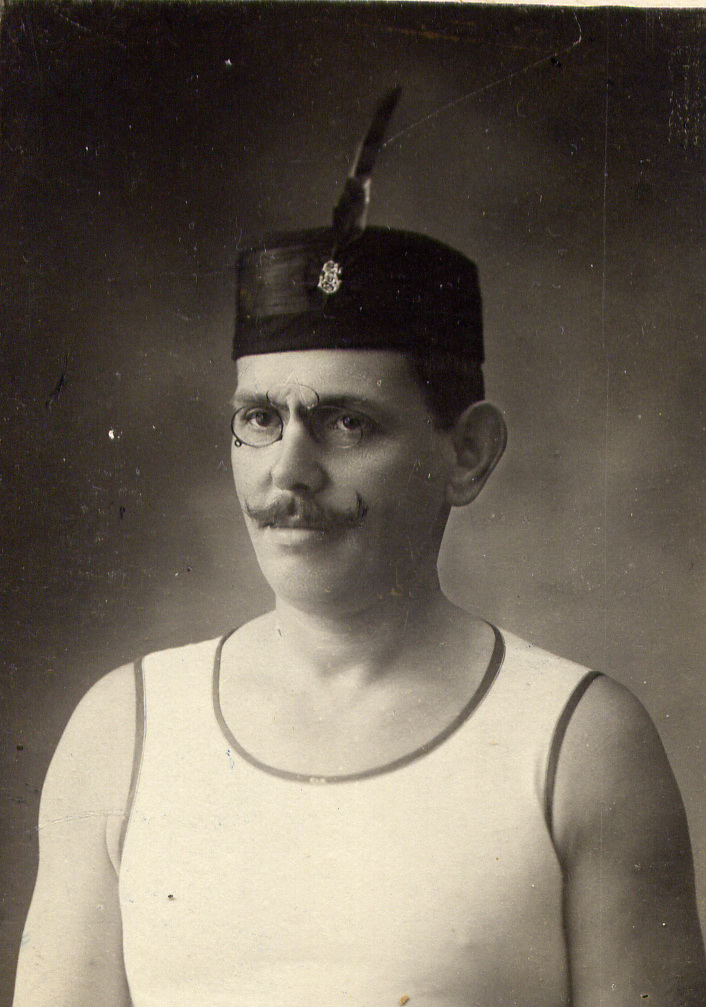
\includegraphics[width=\textwidth]{img/01_pechan.jpg}
  \caption*{Br. Jaroslav Pechan, zakládající člen jednoty, foto: archiv T.~J. Sokol Libeň}
  \end{subfigure}
  \hfill
  \begin{subfigure}{0.45\textwidth}
   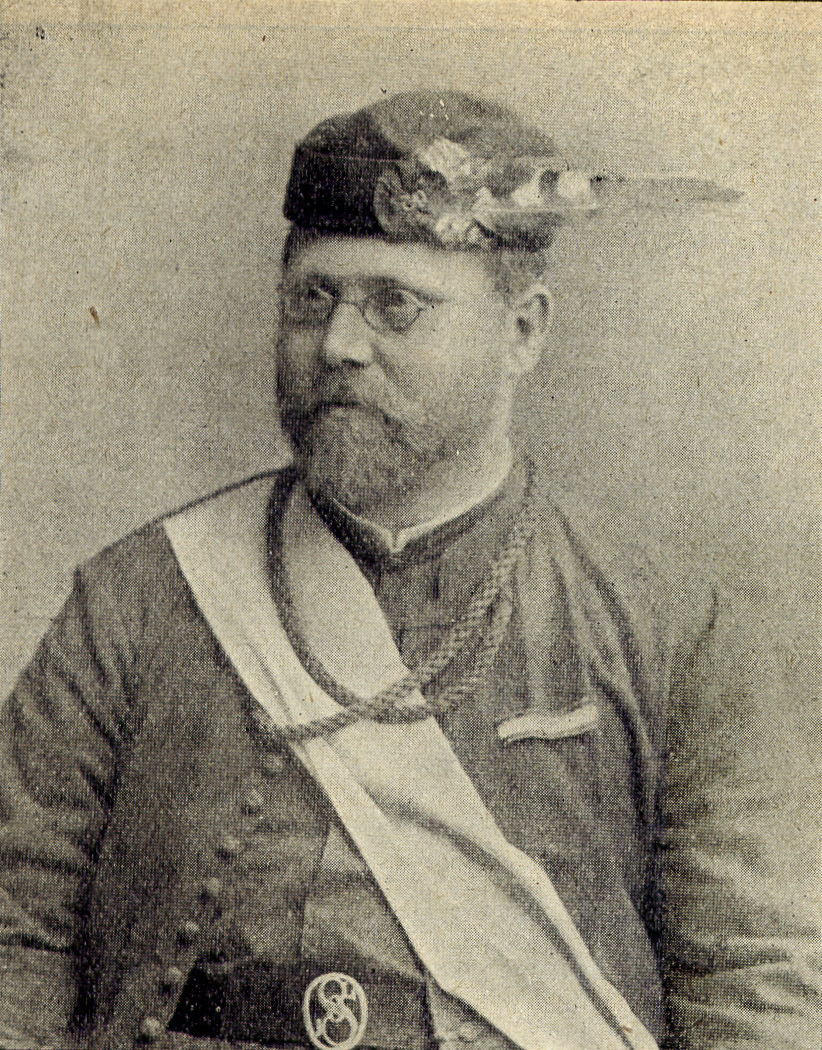
\includegraphics[width=\textwidth]{img/02_klazar.jpg}
  \caption*{JUC. Václav Klazar, první náčelník T.~J. Sokol Libeň (1884–⁠⁠⁠⁠⁠⁠1890) a druhý starosta (1895–⁠⁠⁠⁠⁠⁠1899), foto: archiv T.~J. Sokol Libeň}
  \end{subfigure}
\end{figure*}

I~u~nás, v~chudém dělnickém prostředí, byla již tehdy německá škola (vliv německých továrních firem) a na dveřích obecního úřadu cedule: "Mluvte česky! Kdo se za svůj jazyk stydí, hoden potupy všech lidí!", kterou tam vyvěsil tajemník obecního úřadu JUC. Václav Klazar, rovněž činný člen Sokola Pražského (od roku 1879). Není tedy divu, že tito mladí idealisté --⁠⁠⁠⁠⁠⁠ a mohl mladý učitel na venkovské škole nebýt
idealistou? --⁠⁠⁠⁠⁠⁠ si uvědomili nejen velký význam a vliv Tyršových
myšlenek, ale i svou učitelskou odpovědnost.

Bylo tehdy v~Čechách a na Moravě po l. všesokolském sletu (1882) již 104 sokolských jednot a v~blízkosti Libně sedm: v~Praze (zal. 1862), v~Karlíně (1867), na Smíchově (1868), ve Vršovicích (1870), v~Záběhlicích (1870), v~Braníku (1871) a na Žižkově (1872), nehledě k~sedmi jednotám v~ostatní Evropě a dvaceti v~USA. Snadné se dohodnout -- nesnadné provést, zvláště v~takovém malém i společensky nevýhodném prostředí. Ale i tady se cesta našla. Dne 8.~září 1884 byla uspořádána v~tehdejším hostinci "U Deutschů" přednáška náměstka náčelníka Sokola Pražského Dr. Františka Čížka o~úkolech a cílech sokolského hnutí. Zúčastnilo se jí kupodivu 118 osob. Řídil ji Tomáš Ronek.


\begin{figure*}[h]
  \centering
  \begin{subfigure}[c]{0.4\textwidth}
   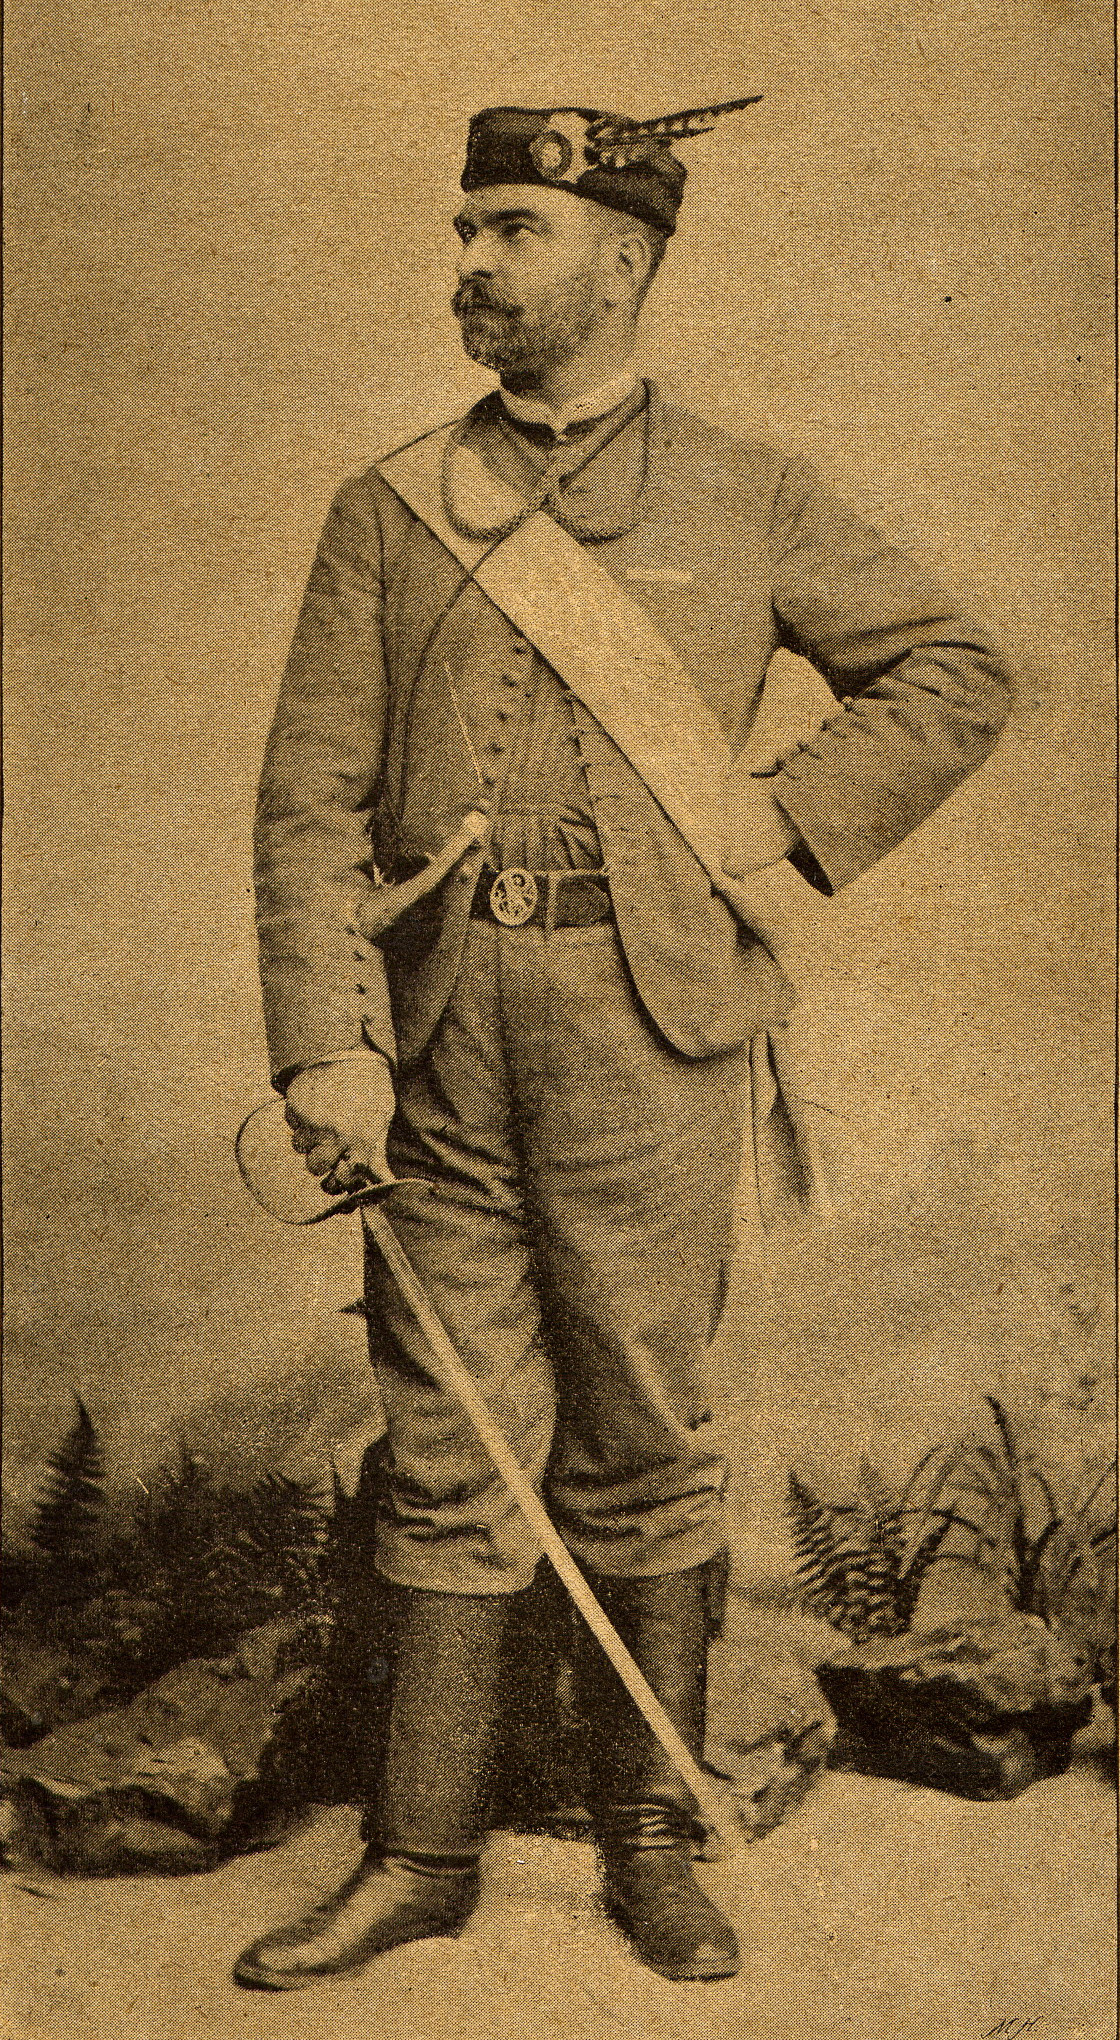
\includegraphics[width=\textwidth]{img/03_cizek.jpg}
  \caption*{Dr. František Čížek, zakládající člen jednoty (1884), foto: archiv T.~J. Sokol Libeň }
  \end{subfigure}
  \hfill
  \begin{subfigure}[c]{0.5\textwidth}
   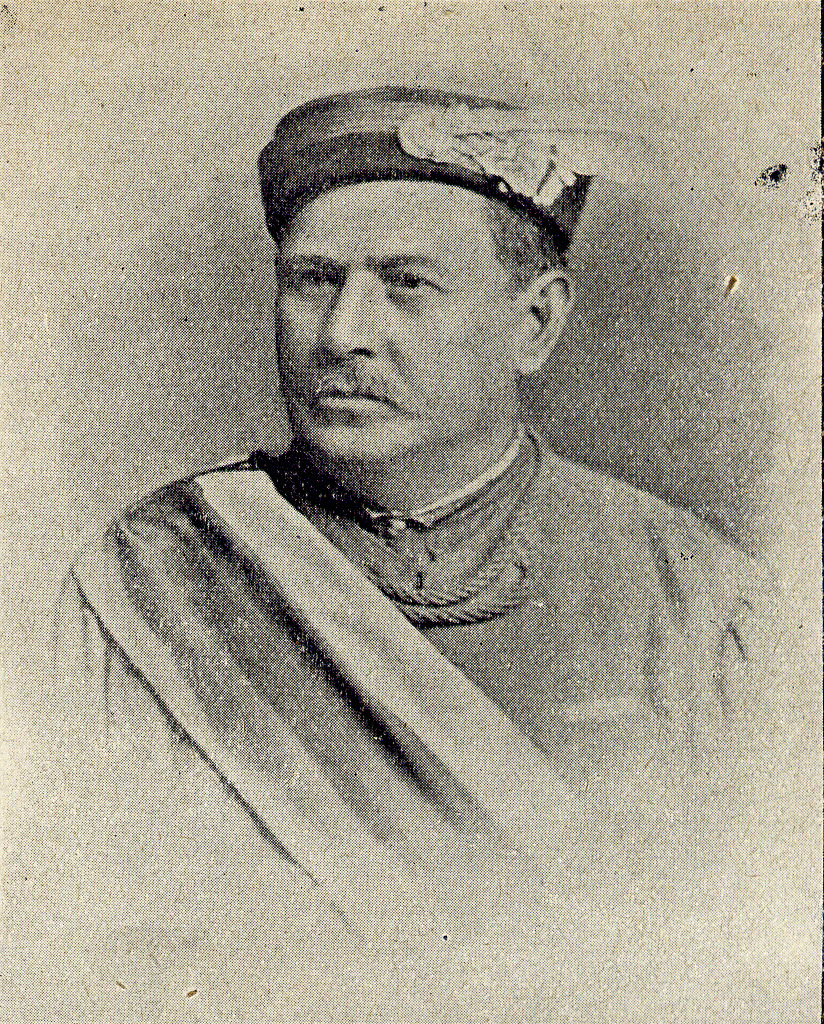
\includegraphics[width=\textwidth]{img/04_voctar.jpg}
  \caption*{Josef Voctář, první starosta T.~J. Sokol Libeň (1884–⁠⁠⁠⁠⁠⁠1894), foto: archiv T.~J. Sokol Libeň }
  \end{subfigure}
\end{figure*}

K~vlastnímu založení T.~J. Sokol v~Libni došlo pak v~ustavující valné hromadě 26.~10. 1884, při níž byl za starostu obezřetně zvolen obecní starosta Josef Voctář, jeho náměstkem "stavitel ve službách obecních" Josef Bukovský, náčelníkem JUC. Václav Klazar, jeho náměstkem učitel Jaroslav Pechan a jednatelem Vítězslav Vondřich. Bylo tedy vedení jednoty svěřeno osobám odborně povolaným, ale i důvěryhodným, neboť ne všemu obyvatelstvu mohlo být vítáno pokrokové zaměření Sokola, bratrské tykání, pozdrav "Nazdar" a dokonce červená košile sokolského kroje.

Cvičit se počalo velmi brzy; již 20.~ledna 1885. Cvičilo se první tři léta v~hostinci u~Deutschů, později se souhlasem místní školní rady ve škole a pro letní cvičení byl získán roku 1887 od obce pozemek ve výměře 200 čtverečních sáhů po 10 haléřích, jenž byl později vyměněn za jiný, o~40 sáhů větší (1 čtvereční sáh odpovídá 3,6\,$\textrm{m}^2$).

Duší tělocvičné činnosti byl od počátku bratr Jaroslav Pechan, později středoškolský profesor tělocviku, horlivý propagátor tělesné výchovy školní i sokolské. Podlehl posléze dlouholeté chorobě, jež přerušovala jeho nadějnou činnost. Byl autorem "Osnov k~vyučování tělocviku na školách středních, díl I." (r. 1905) a "Tělocviku pro obecné školy chlapecké na základě soustavy Miroslava Tyrše, díl I." (r. 1888). O~Pechanových vlastnostech a zásluhách můžeme číst v~"Památníku 25letého trvání T.~J.  Sokol v~Praze-Libni 1884–⁠⁠⁠⁠⁠⁠1909" z~pera Františka Glimana a Památníku z~roku 1934 z~pera Ladislava Vernera, dvou jeho současníků a spolupracovníků. Pozdější místonáčelník jednoty, všestranný umělec, český básník, autor "Sokolských sonetů" a odborný sokolský tělocvičný spisovatel Karel Hlaváček (1874–1898) o~něm napsal: "Na prvním místě bije do očí jeho neúnavná činnost, která vrcholí ve dnech župního sletu roku 1886, kdy bydlil dávno již na místě vzdáleném a přece svou pevnou rukou ovládal a řídil přípravné kroky. Byl vychovatelem sokolských  charakterů.  Chválím si bratra Pechana jako bystrovtipného organizátora, jenž řady všech odborů upevnil tuhou kázní řádů zocelil a utužil. Bude vždy mezi předními, jež slaviti a vzpomínati budeme jako muže o~jednotu zasloužilé." Roku 1889 tento v~tělocviku odborně kovaný J. Pechan je již náčelníkem Sokola Vinohradského. Jeho duch v~cvičitelském sboru opravdu na dlouho přetrval jeho odchod. Zemřel 14.~6. 1915 v~Praze a pohřben byl na Vinohradském hřbitově.

\begin{figure*}[h!]
  \centering
   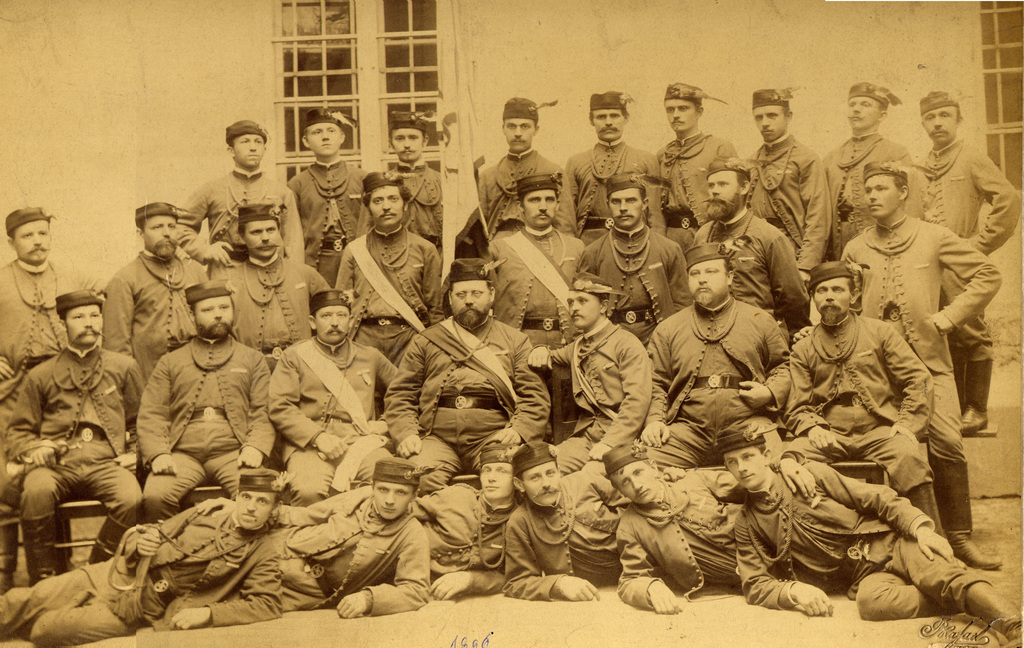
\includegraphics[width=0.9\textwidth]{img/05_zakladajici_clenove_1886.jpg}
  \caption*{Členové jednoty v~roce 1886, uprostřed s~plnovousem JUC. Václav Klazar, t. č. náčelník, a ve druhé řadě druhý zprava starosta Josef Voctář; foto: archiv T.~J. Sokol Libeň}
\end{figure*}

{\sloppy Vedle pravidelného cvičení od počátku byl pěstován i život společenský. Téměř pravidelně byly pořádány tradiční sokolské šibřinky u~Deutschů, nebo v~pivovarnickém sále (v~některých letech nahrazeny subskripcí rozmnožující finanční prostředky jednoty), čajové večírky, z~nichž jeden navštívil sám Mikoláš Aleš. Pěstovány byly též přátelské styky s~jinými jednotami (společný výlet do Kunratic se Sokolem Pražským roku 1886). Členové se navštěvovali v~jednotách, účastnili se pohřbů známých a zasloužilých osob (např. Dr. Ed. Grégra, přenesení ostatků P. J. Šafaříka, Jana Kollára apod.). Do pravidelné činnosti jednoty patřily každý rok četné výlety, krátké, delší, denní i noční. Bývaly spojeny příznačně pro tu dobu s~různými slavnostmi, veřejným cvičením apod. jako akce národně vlastenecké a společenské zároveň utužující vzájemnou, tehdy tak potřebnou, pospolitost vskutku bratrského ducha a posilující i tělesně. Účastnil se jich také někdy trubačský sbor jednoty založený již roku 1886. Tento trubačský sbor sdílel za sbormistrů Arona, Šerkse a Šillera téměř deset let osudy jednoty na nestálé a kolísavé vlně práce, úspěchů a přízně i horlivosti členů. Již roku 1887 si stěžuje kronikář, že vojenské odvody jeho řady prosívají na čtvrtinu. Nakonec se sbor v~roce 1895 rozešel. Roku 1904 byl sice na čas vzkříšen, ale skutečné obnovy se dočkal až v~roce 1910. \par}

\begin{figure*}[h!]
  \centering
   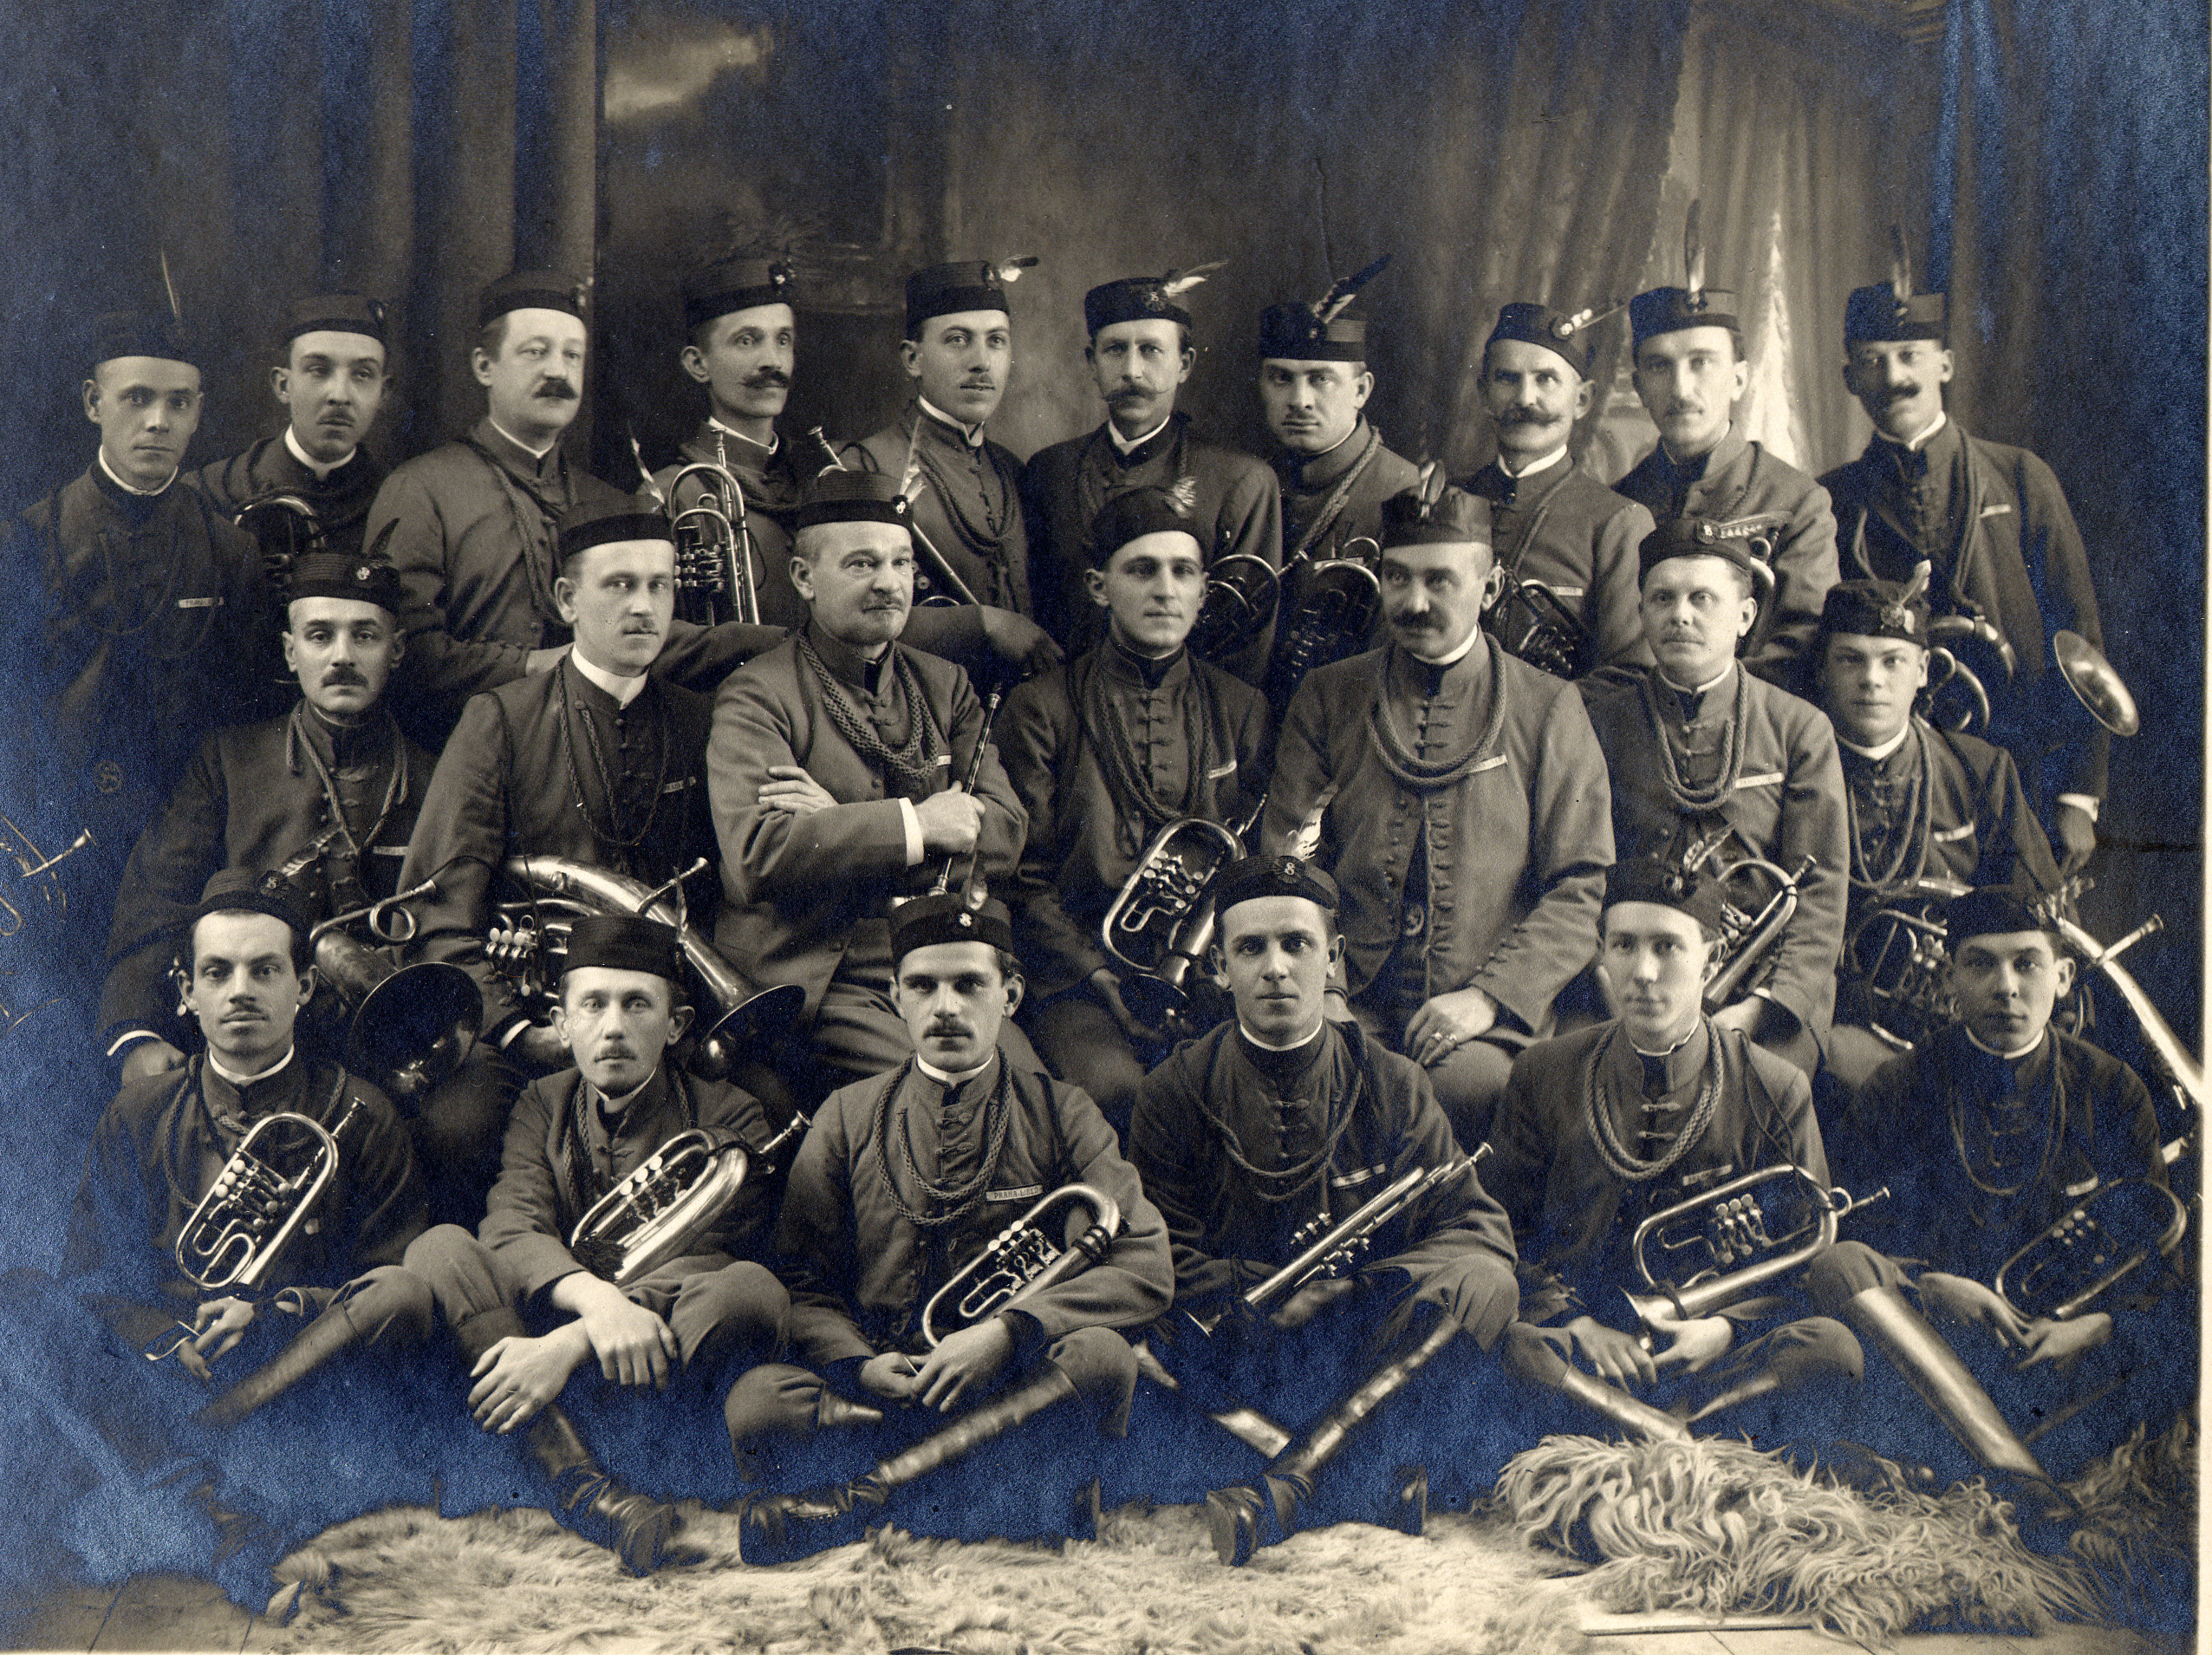
\includegraphics[width=0.9\textwidth]{img/06_trubaci.jpg}
  \caption*{Trubačský sbor jednoty (1886), foto: archiv T.~J. Sokol Libeň}
\end{figure*}

Časté byly též zájezdy do jiných měst a jednot při nejrozmanitějších příležitostech (např. 1893 zájezd do Polska, 1898 Palackého oslavy v~Hodslavicích, 1900 zájezd ČOS do Olomouce, 1903 slet v~Českých Budějovicích, 1905 Vídeň, 1906 \mbox{Záhřeb} aj.). V~posledních letech tohoto období došlo k~úspěšnému pravidelnému pořádání členských besed s~hodnotnou náplní a hojných vycházek v~našem hlavním městě s~návštěvami památek a uměleckých výstav.

Již od vzniku jednoty byly pěstovány přátelské styky také s~rozličnými libeňskými spolky a organizacemi: spolkem "Osvěta-Omladina", s~"Věnceslavem", který vystupoval často i na podnicích jednoty i při zájezdech, "Ústřední maticí školskou" aj. Byla to vůbec doba všestranné nadšené veřejné práce, jež dovedla roku 1889 tři sokolská závodní družstva s~JUDr. Janem Podlipným, přes výslovný osobní zákaz samého c. k. místodržitele, do Paříže pro první tři ceny v~mezinárodních závodech družstev v~tělocviku. V~prvním družstvu byl také spoluzakladatel libeňského Sokola Jaroslav Pechan.

Cvičilo se, někdy s~obtížemi, u~Deutschů, pak v~libeňských školách, když došlo k~neshodám s~hostinským. Cvičilo se i na prostorách kolem sokolovny (po jejím postavení, dnes zahrádka a garáže; \pozned{dnešní dvůr a zahrada sokolovny, pozn.~ed.}) nebo na letním cvičišti za "starou hospodou" (1900). Nebyly vždy radostné chvíle také při úvahách, kde cvičit – ale vždy uspěl lidský rozum a pocit odpovědnosti. 

Po organizační stránce měla jednota v~župní organizaci (župní zřízení zavedeno v~Sokole právě roce 1884) své místo v~župě Středočeské a teprve po ustavení České obce sokolské (1889), jejímž prvním starostou byl právě u~nás v~Libni dobře známý JUDr. Jan Podlipný (starosta města Prahy, první starosta Všeslovanského sokolstva), byla přeřazena do župy Barákovy \pozned{(dnes je naše jednota opět součástí župy středočeské J. Podlipného, pozn. ed.)}. V~jejím vedení se vždy dobře uplatňovala. Cvičitelské kurzy pro cvičitele všech složek jednoty, konané v~rámci župy a jednoty, přispívaly k~potřebné odborné úrovni vší práce v~jednotě.

Roku 1896 upravena v~sokolstvu péče o~jednoty v~menšinách, založen základ (fond) pro stavbu menšinových sokoloven a určeny vznikajícím a malým jednotám ve zněmčeném pohraničí tzv. ochranitelky. Byla to nutná pomoc těžce, ale odvážně zakládaným jednotám. Sokolské jednotě v~Libni také přidělena "chráněnka" – jednota v~hornických Kopistech u~Mostu, kde snad nebylo ani 200 domů a necelých 2000 obyvatel, jen z~poloviny Čechů. Osada ta patřila mezi nejstarší a nejdůležitější v~celém kraji. Zanikla roku 1979, kdy musela ustoupit uhelným dolům. Jednotu v~Kopistech libeňští pravidelně podporovali, každého jejího podniku se zúčastnili a v~letech 1899 a 1904 k~ní uspořádali hromadné výlety. Roku 1906, kdy se v~Kopistech konal slet župy Krušnohorské, se z~Libně zúčastnilo 35~mužů a 6 žen, v~čele se starostou F. Filipem.

\begin{figure*}[h!]
  \centering
   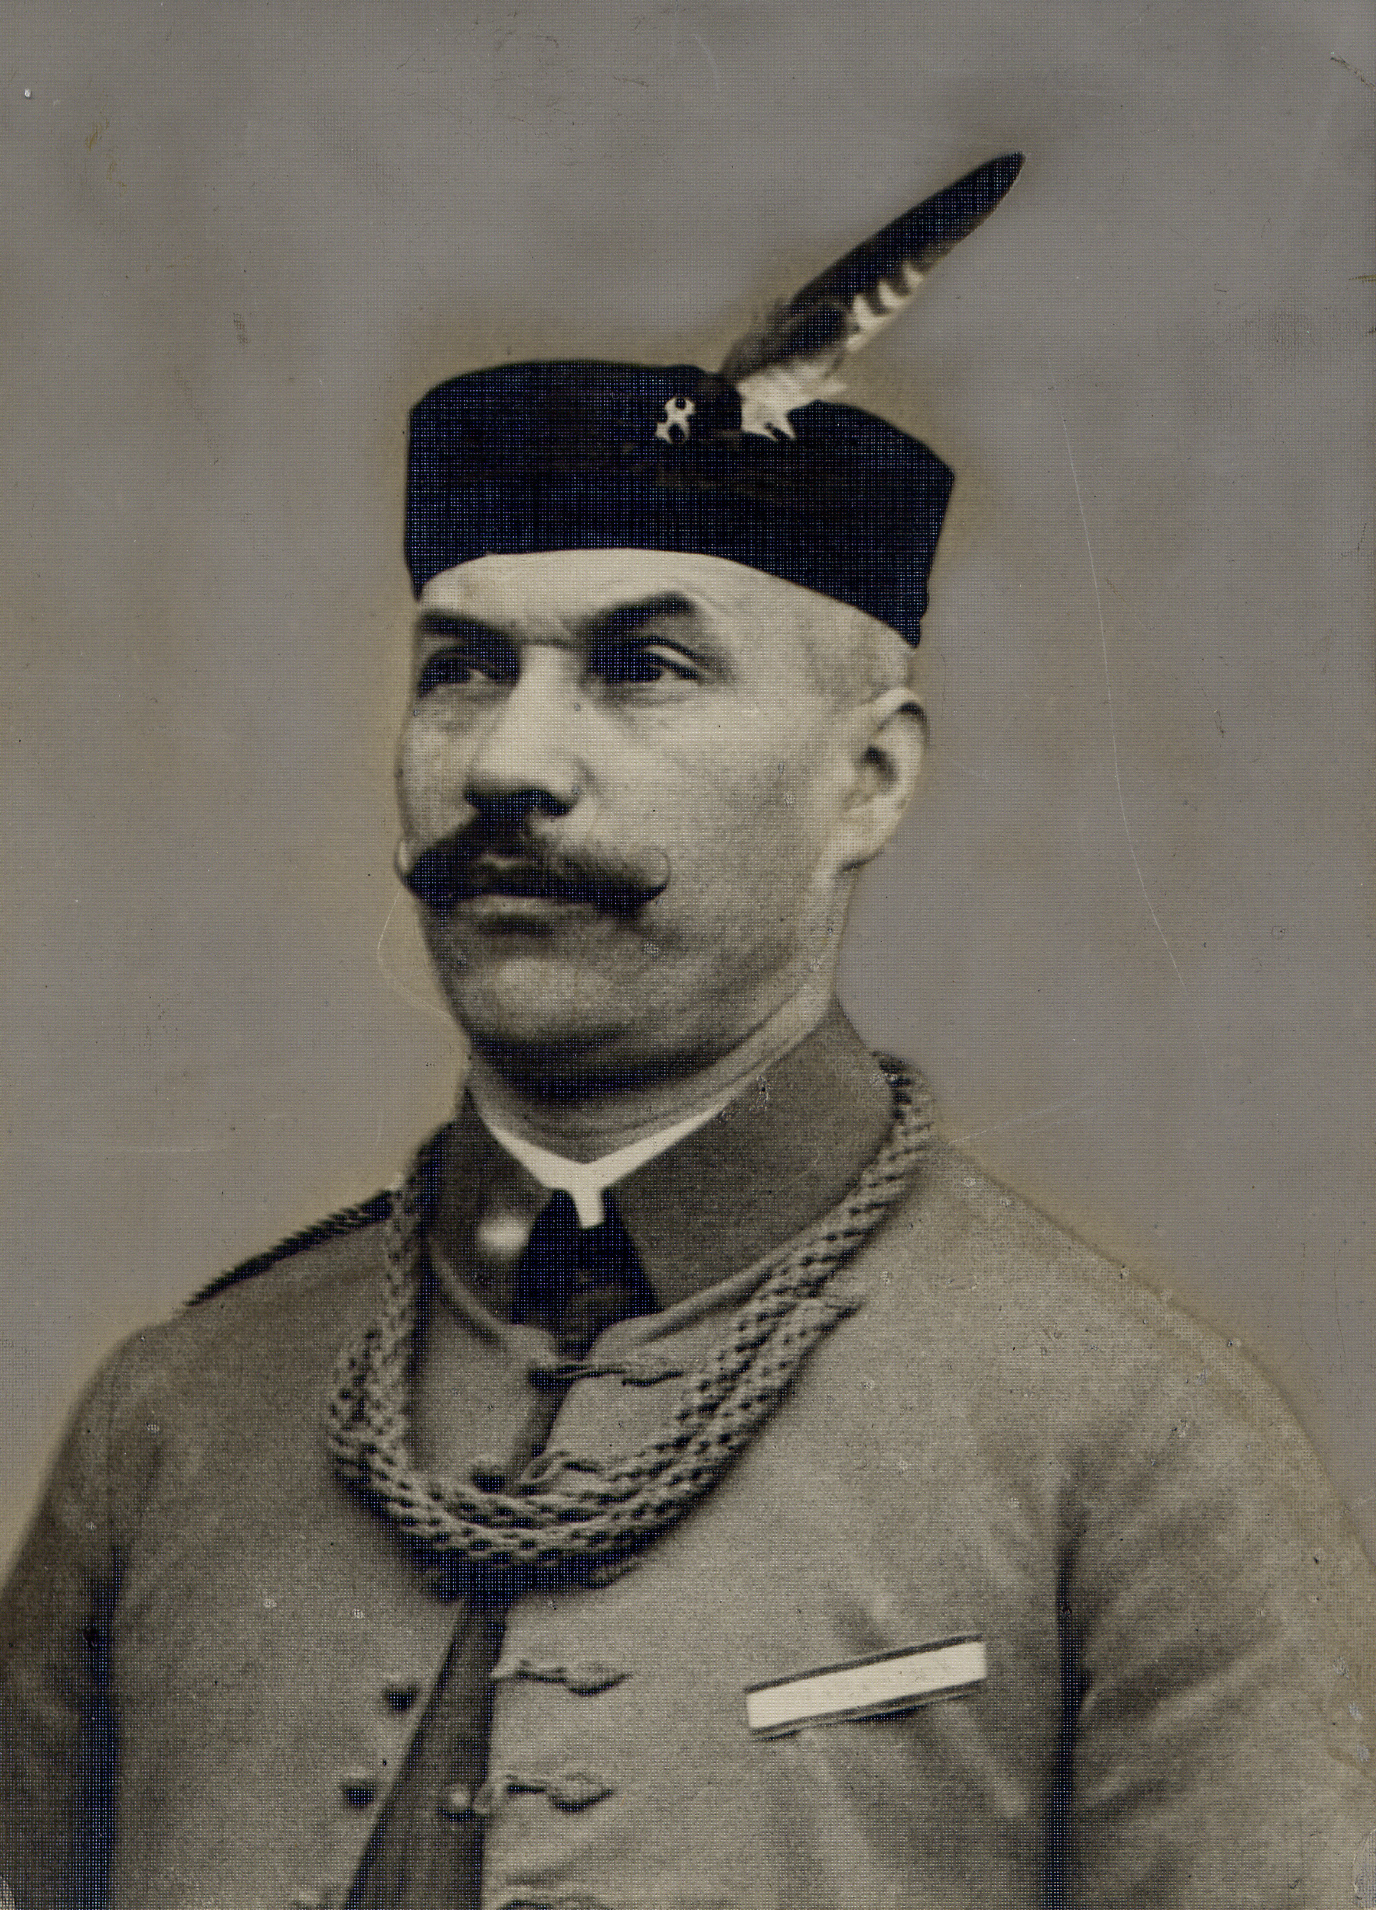
\includegraphics[width=0.4\textwidth]{img/07_filip_starosta.jpg}
  \caption*{Br. František Filip, třetí starosta jednoty (1900–⁠⁠⁠⁠⁠⁠1920); jeho zásluhou byla postavena sokolovna, foto: archiv T.~J. Sokol Libeň}
\end{figure*}

\subsection{První cvičení u~Deutschů}
Zmínili jsme se již o~I. sletu (1882), který se konal na Střeleckém ostrově za osobního řízení Dr. M. Tyrše. Slet přispěl ke vzniku nových sokolských jednot a tak se zrodil i Sokol v~Libni. Přinášíme obrázek hostince u~Deutschů (stál v~místech nynějšího divadla Pod Palmovkou), kde se konala 26.~října 1884 ustavující valná hromada a kde první tři roky mladá sokolská jednota cvičila. Už v~prvních cvičeních zde nastupovala tři desetičlenná družstva – bylo to 20.~ledna 1885 a již 31.~ledna zde uspořádali první šibřinky. Měly ráz: "Praha a okolní obce za sto let". Kronikář Glimann píše: "Výtěžek Šibřinek byl značný. Tak mělo konečně členstvo svoje nářadí a my řadu členů a příznivců více".

V~roce 1886, tj. dva roky po založení jednoty, se konal v~Libni na Knoblochově louce (Libeň tehdy byla ještě vesnicí) župní slet. Byl velmi zdařilý, protože cvičitelský sbor vedený ještě Jaroslavem Pechanem, pracoval naprosto spolehlivě. Je úžasné, co mladá jednota všechno stihla. Těch výletů, doložených "Výletními listy", těch okrskových a župních veřejných cvičení, vše většinou v~sokolských krojích. Besedy s~přednáškami, šibřinky, letní zábavy, čajové večírky aj.
\begin{figure*}[h!]
  \centering
  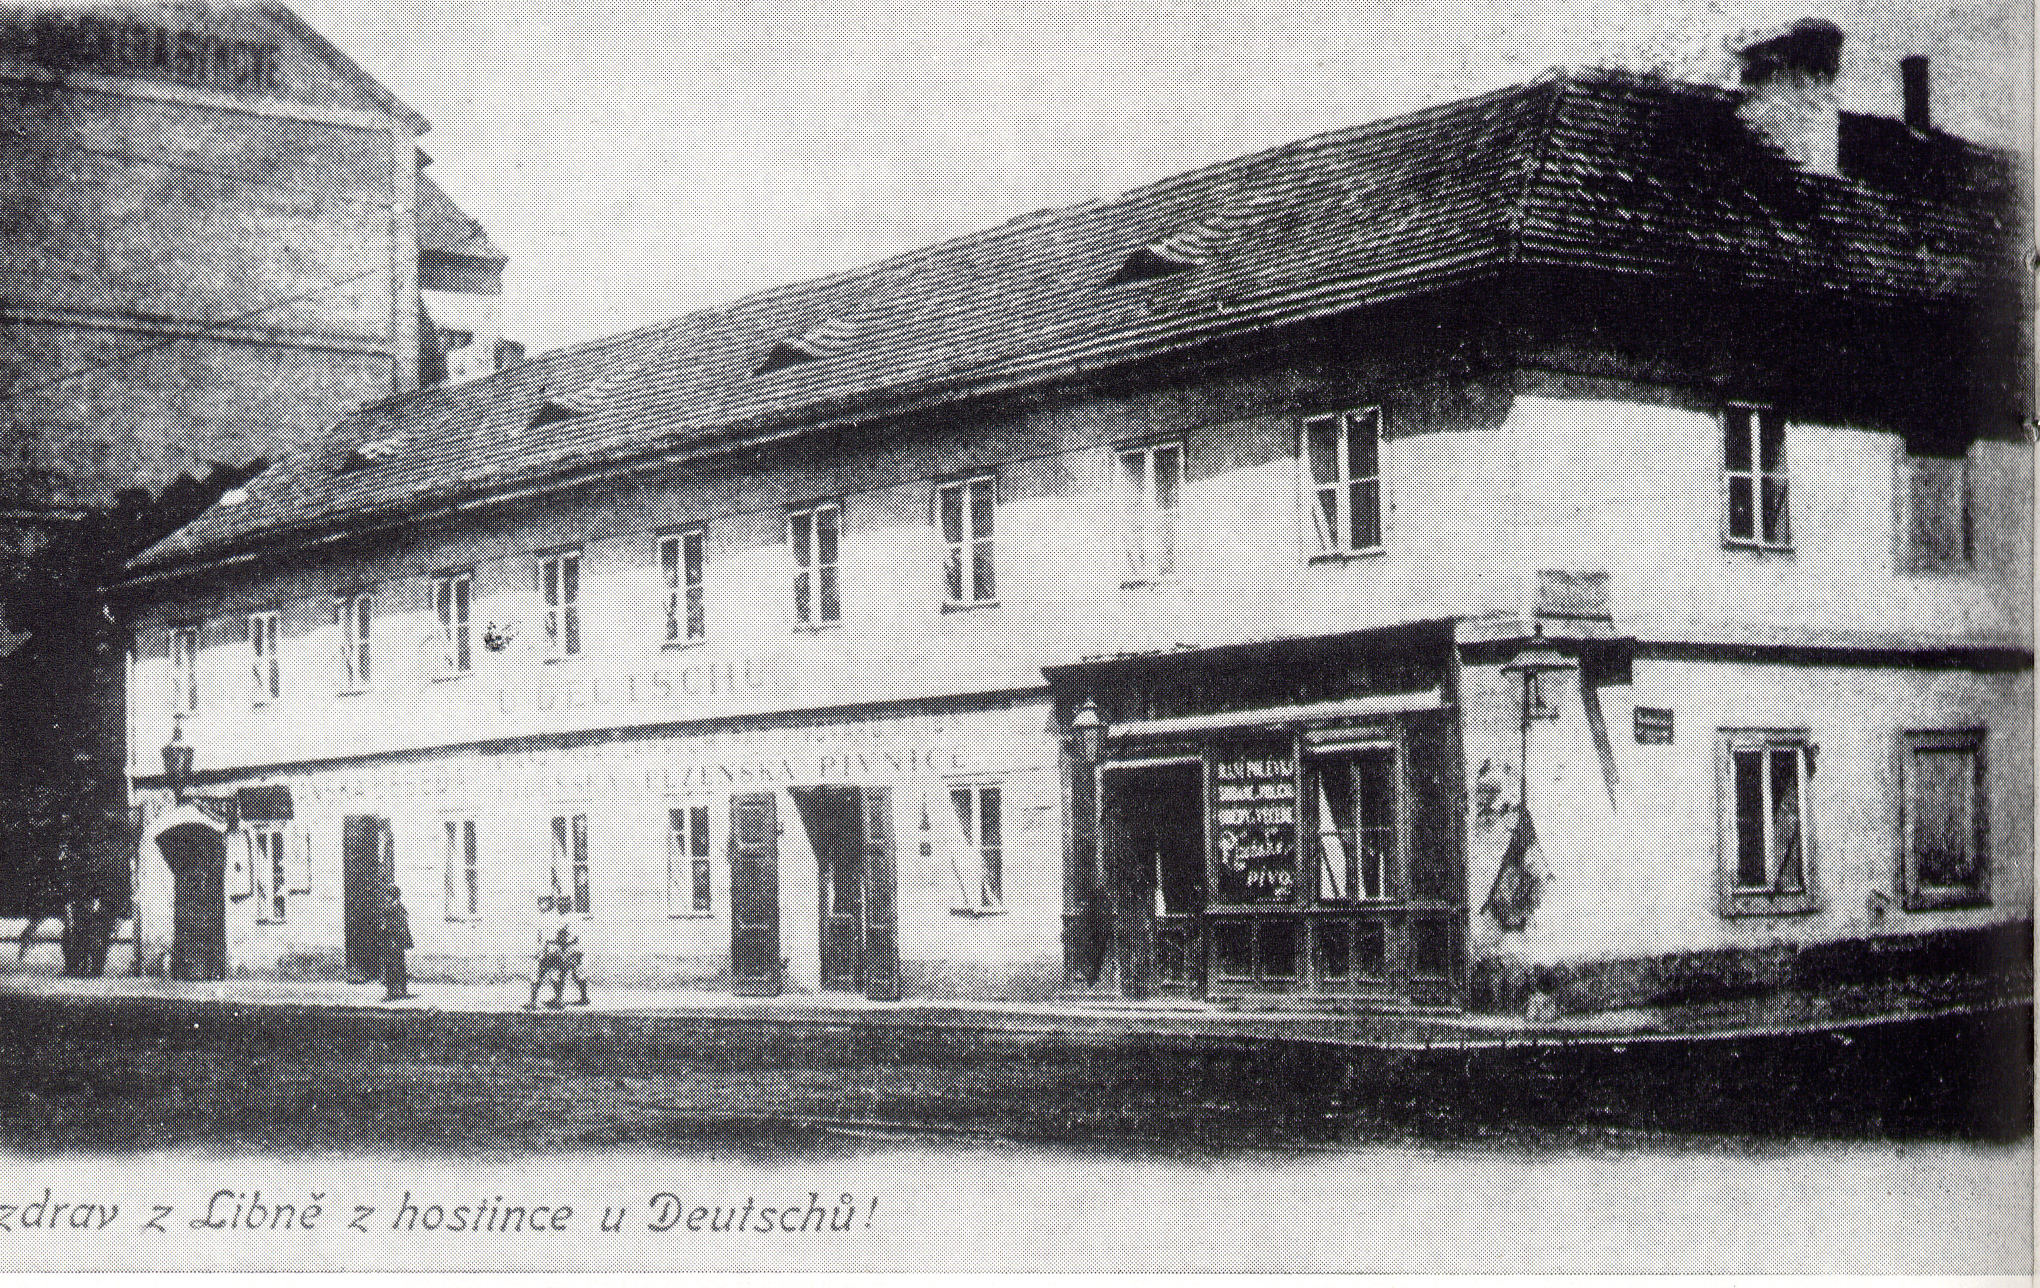
\includegraphics[width=\textwidth]{img/09_hospoda_u_deutschu.jpg}
  \caption*{Hostinec u~Deutschů (1884), pohlednice z~archivu T.~J.
  Sokol Libeň}
\end{figure*}

Na sklonku roku 1889 začíná v~Libni, podobně jako v~jiných jednotách, cvičení mužského dorostu. Rozrůstá se hlavně v~roce 1893, kdy se v~květnu přihlásilo přes 40 učňů. Cvičili za vedení br. Josefa Decastella \pozned{(otce pozdější náčelnice a pamětnice Věry Decastellové (1919–2014); její vyprávěné vzpomínky jsou uloženy v~archivu jednoty, pozn. ed.)}. To už se necvičilo v~hostinci, ale v~tělocvičně nové školy proti zámku. Správní výbor Sokola se začal zabývat myšlenkou stavby sokolovny a zřídil Fond pro stavbu sokolovny a začalo se usilovně šetřit dokonce ve vybraných hostincích byly umístěny malé "haléřové" pokladničky.

\textbf{II. všesokolský slet (1891)} se konal v~Královské oboře \pozned{(dnešní Stromovka, pozn. ed.)} u~příležitosti Jubilejní výstavy. Náš kronikář br. Glimann o~tom píše: "Nemám tak obratné pero, abych mohl býti tlumočníkem onoho rozruchu slavnostního, onoho posvátného rozechvění a citu hrdosti, jež se nás všech zmocnily při projevech spontánního nadšení, jakým každá nová meta vzorného výkvětu našich junáků borců byla přijata." Dodejme jen, že z~Libně na II. sletu cvičilo 24~mužů a v~průvodu šlo 40 členů v~kroji. Na tomto sletě již cvičil jako dvacetiletý Josef Decastello.

V~krátkém mezidobí sletovém (4 roky) se konal znamenitý slet v~Českých Budějovicích (1893) a v~Libni veliká slavnost odhalení druhého sokolského praporu (\pozned{současný hlavní prapor jednoty, který se dochoval a je uschován v~našem archivu; jeho repliku pravidelně používáme, pozn. ed.}). Záštitu nad slavností na zámeckém nádvoří převzala obec libeňská, slavnostním řečníkem byl JUDr. J. Podlipný a Libeň byla slavnostně vyzdobena.

\begin{figure*}[h!]
  \centering
  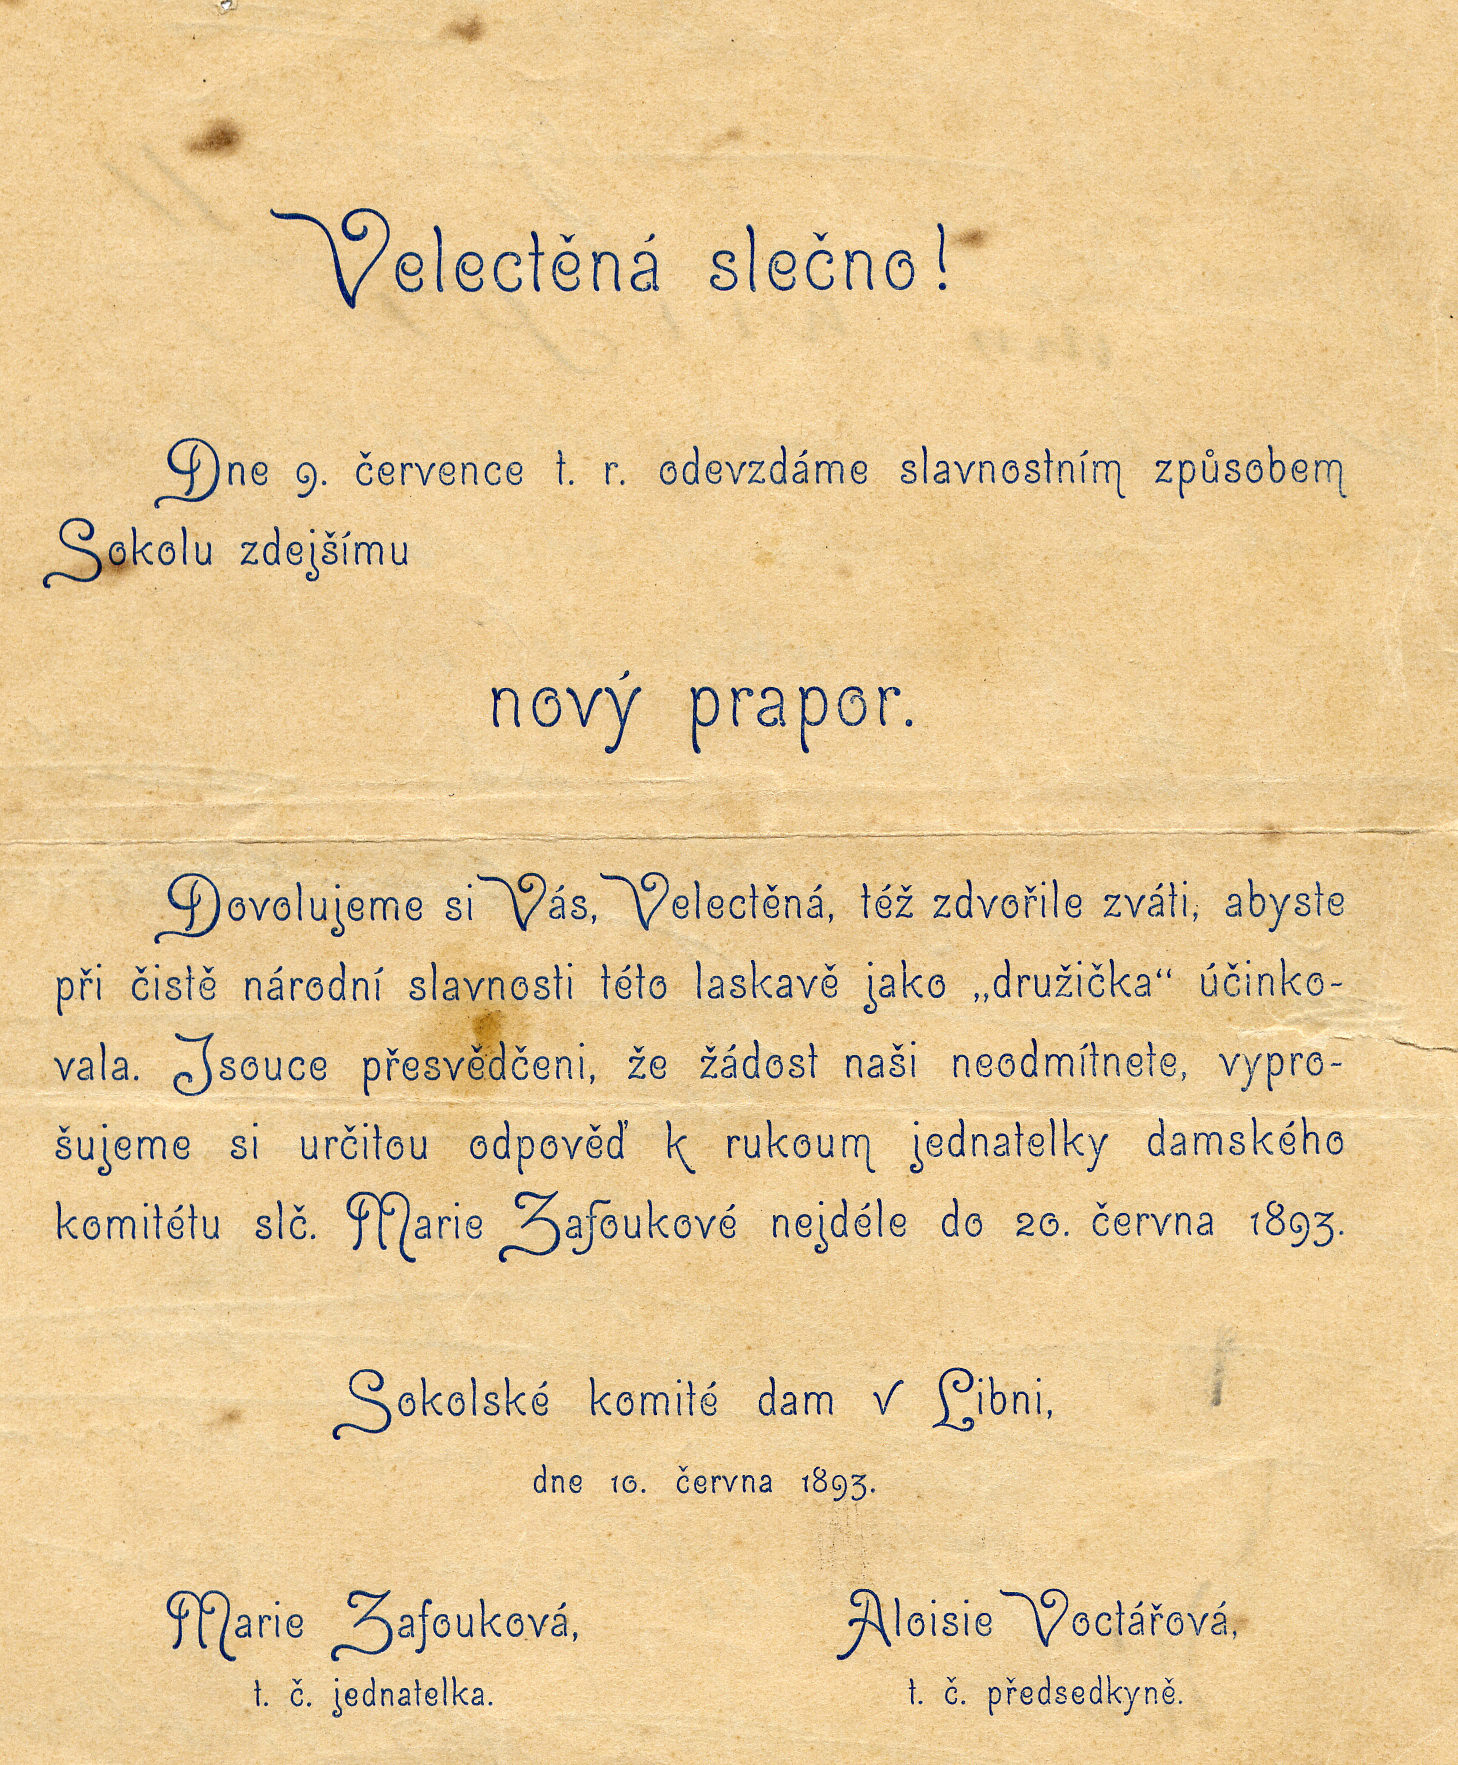
\includegraphics[width=0.55\textwidth]{img/10_pozvanka_prapor.jpg}
  \caption*{Pozvánka na slavnostní odhalení nového praporu (1893), archiv T.~J. Sokol Libeň}
\end{figure*}

\textbf{III. všesokolský slet (1895)} se konal na Letenské pláni, u~příležitosti Národopisné výstavy lidu československého. O~slet byl veliký zájem, a tak již nemohlo stačit místo minulého sletu v~Královské oboře a našlo se lepší. Na Letné se upravil prostor pro 4\,000 cvičenců a tribuny pro 11\,000 diváků. Sokol Libeň poslal do sletového průvodu 57 mužů v~kroji a 10 krojovaných na koních. Cvičilo 28 mužů a také 28 dorostenců. Naše závodní družstvo získalo přes 71\,\% bodů, v~družstvu byl nejlepším br. Decastello (32,10 bodů ze 40). Oba slety (II. a III.) připravil a vedl náčelník Josef Svoboda a jeho náměstek Václav Steiner. V~mezisletovém období zorganizovala ČOS veliký zájezd na Moravu do Hodslavic a později i do dalších míst. V~Libni byl v~roce 1898 založen ženský odbor. Prvního cvičení se zúčastnilo 26 žen. První náčelnicí byla zvolena sestra Růžena Vocetková, jednatelkou Hana Němečková, provdaná Decastellová. V~roce 1901 již naše ženy cvičily na IV. sletu. Smutnou událostí toho roku bylo, že zemřel místonáčelník, básník a spisovatel Karel Hlaváček.

\begin{figure*}[h!]
  \centering
  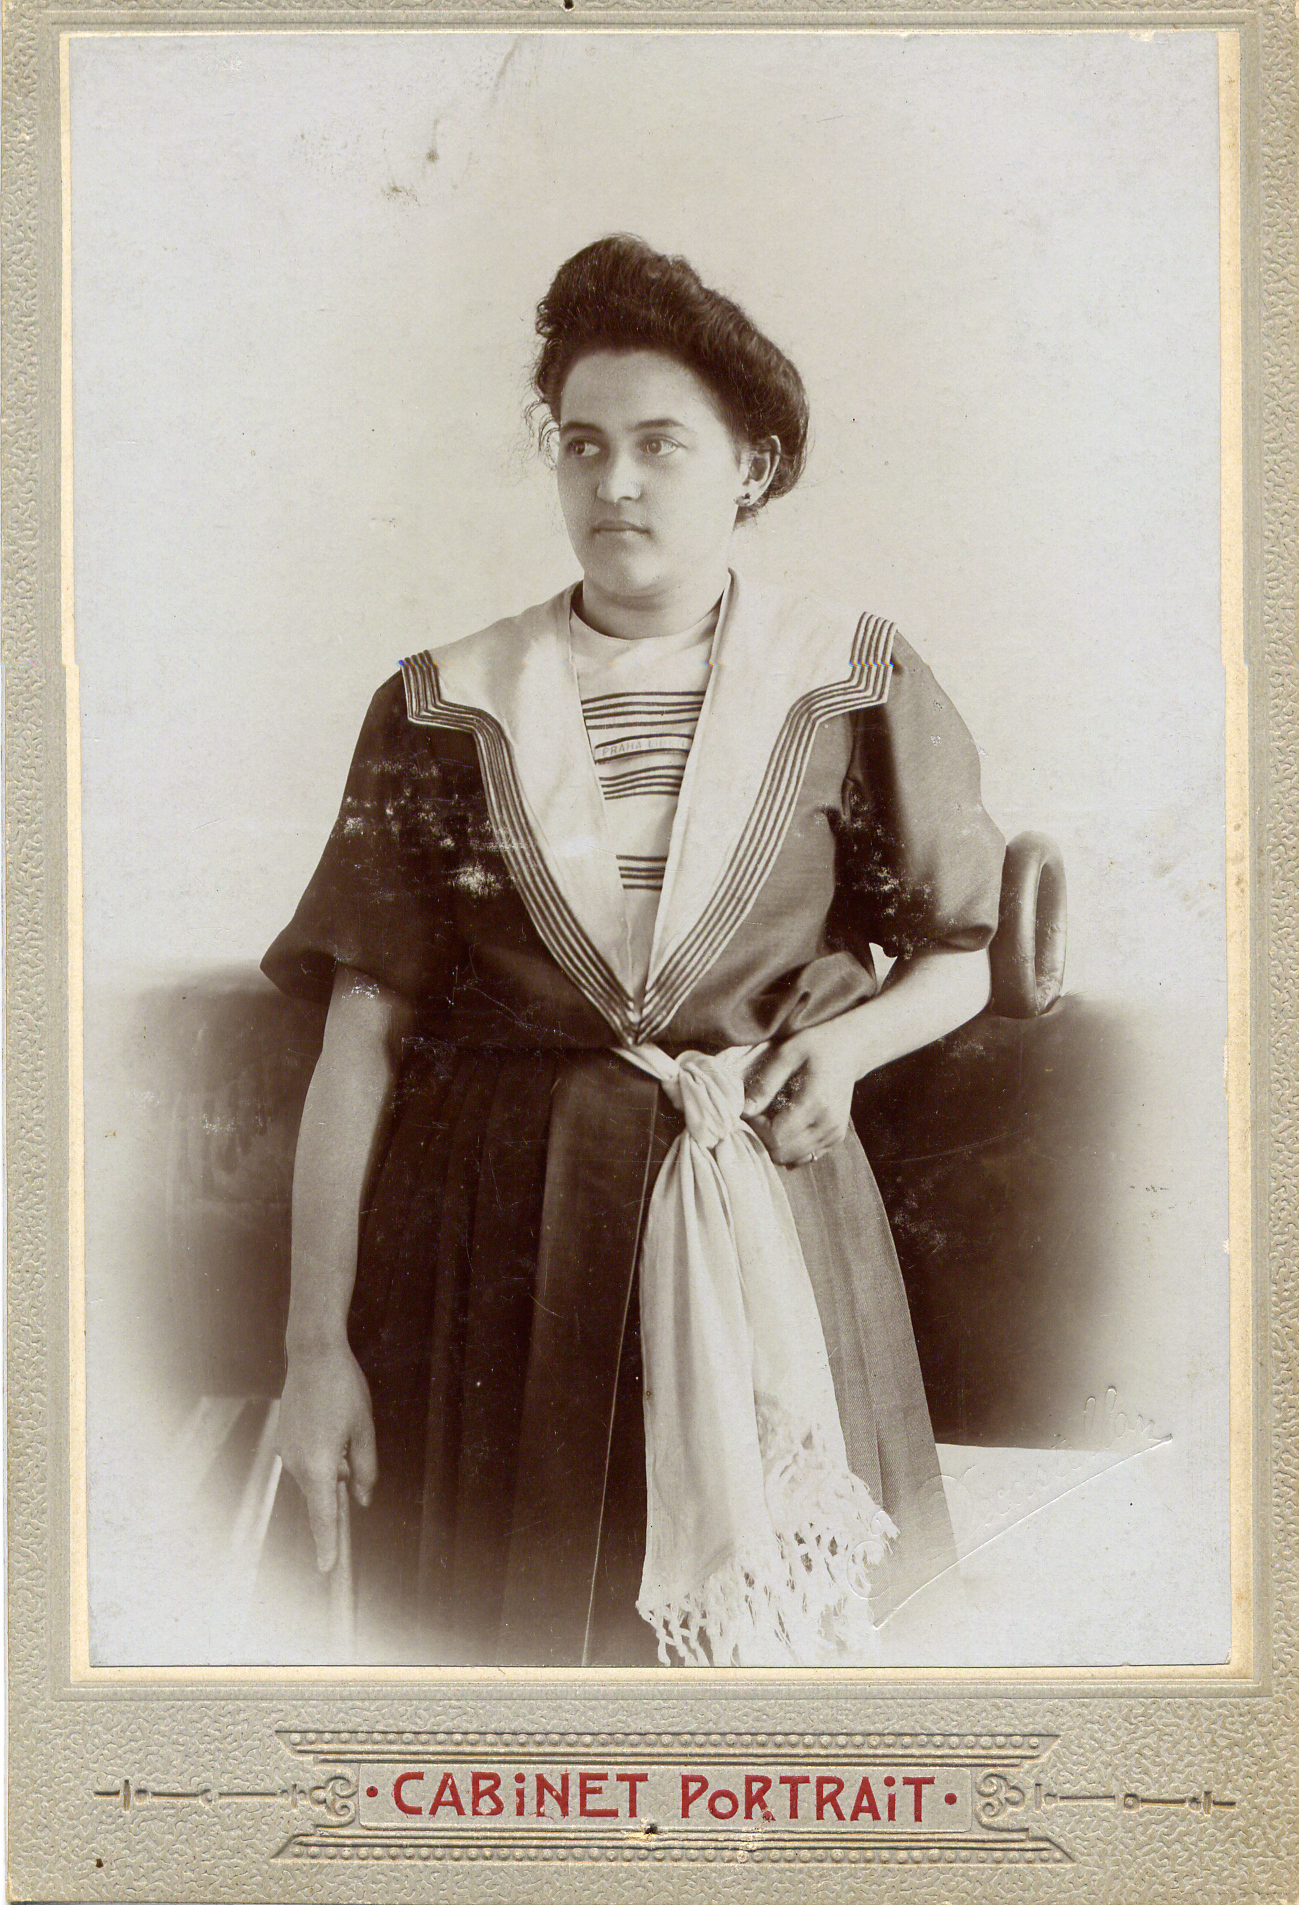
\includegraphics[width=0.45\textwidth]{img/11_hana_decastellova.jpg}
  \caption*{Hana Němečková, vdaná Decastellová, první jednatelka odboru žen a pozdější náčelnice, foto: archiv T.~J. Sokol Libeň}
\end{figure*}

\textbf{IV. všesokolský slet (1901)} se opět konal na Letenské pláni. Před ním se v~Libni konal 2.~6. 1901 župní slet na Pánkově poli, tj.prostor mezi dnešní ulicí Novákových a Na Žertvách. Cvičilo zde 37 družstev na různých nářadích, svážených dlouho do noci z~okolních jednot. Dorostenců bylo přes sto a cvičili v~jedenácti družstvech, z~Libně 25 dorostenců ve 3 družstvech a 15 žen ve 2 družstvech.

\begin{figure*}[hp]
  \centering
  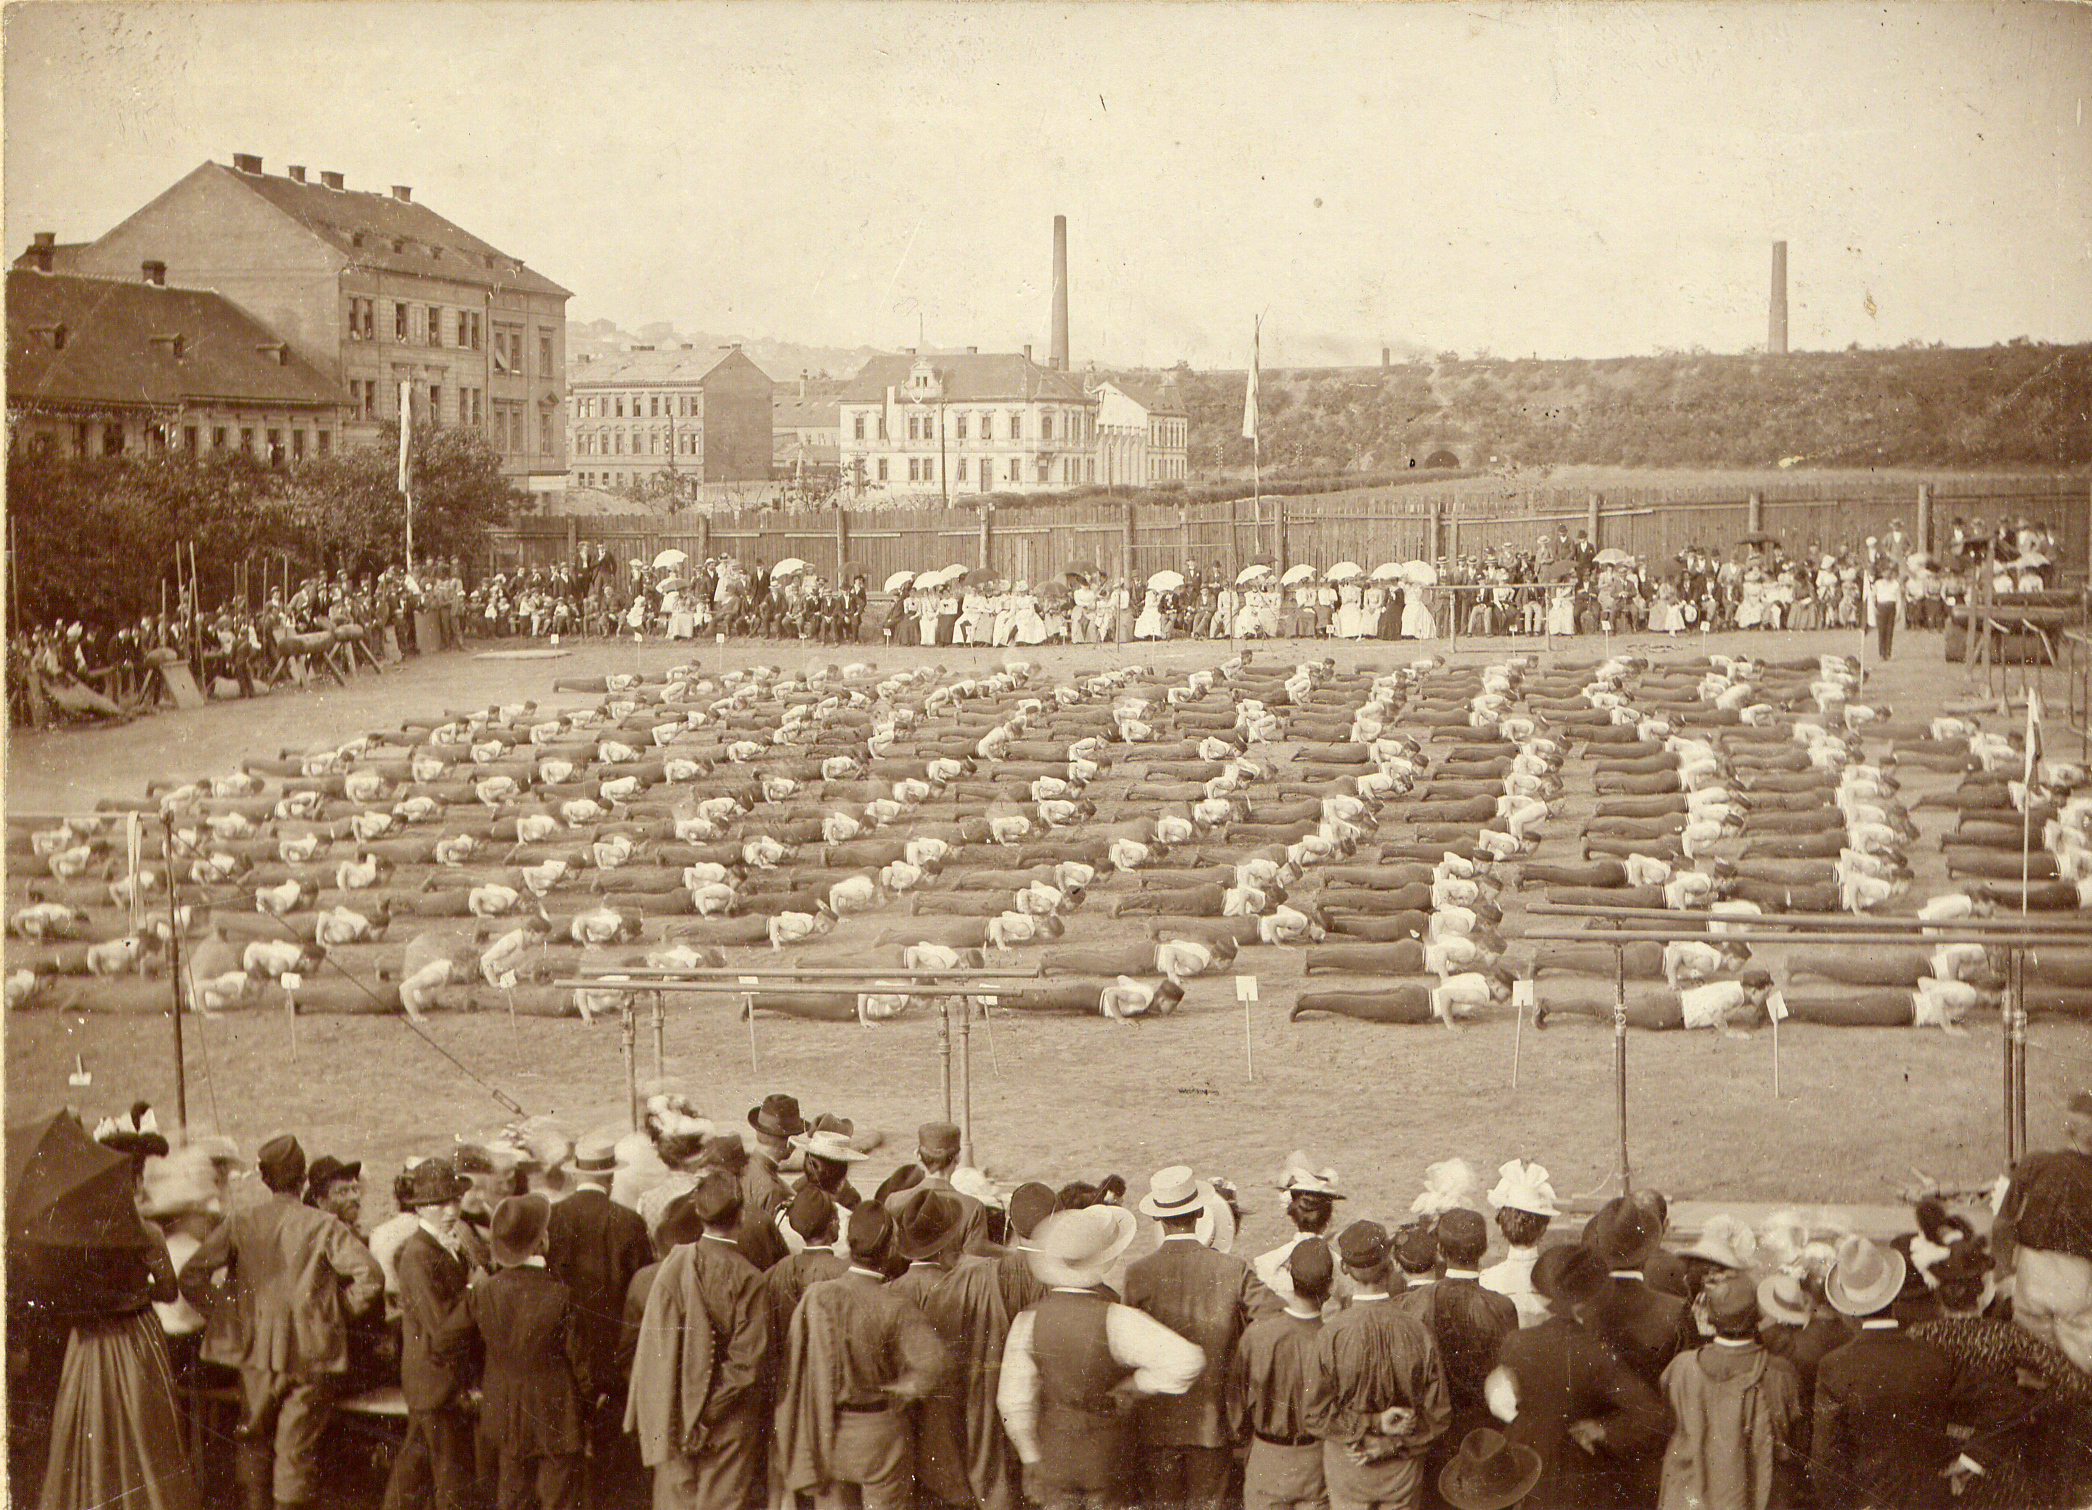
\includegraphics[width=0.9\textwidth]{img/12_na_zertvach.jpg}
  \caption*{Veřejné cvičení v~ulici Na Žertvách (1901; v~pozadí železniční násep, na jehož místě nyní stojí mosty na Balabence), foto: archiv T.~J. Sokol Libeň}
\end{figure*}

\begin{figure*}[hp]
  \centering
  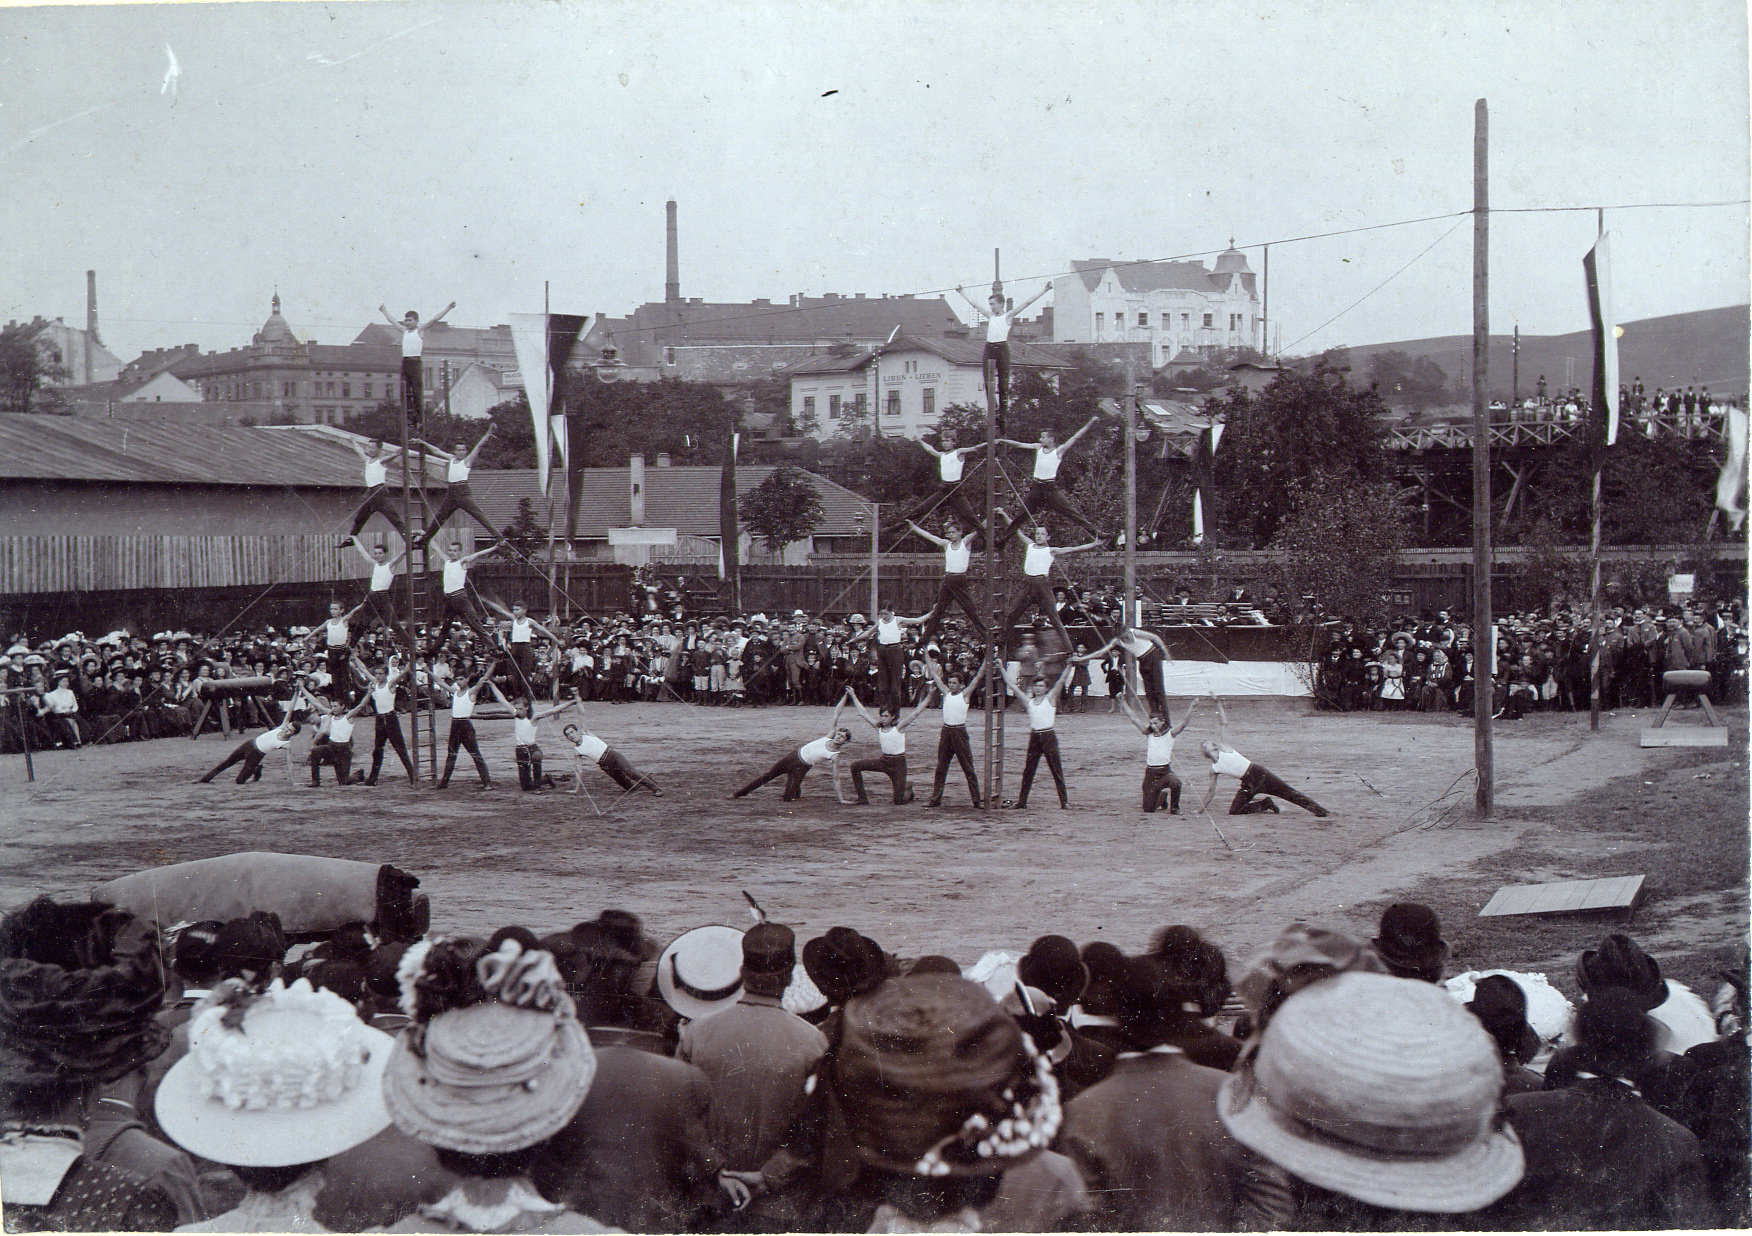
\includegraphics[width=0.9\textwidth]{img/13_verejne_cviceni.jpg}
  \caption*{Veřejné cvičení v~dnešní Voctářově ulici (1901; v~pozadí nádražní budova libeňského dolního nádraží a dodnes stojící dům na rohu Sokolovské a Zenklovy ulice), foto: archiv T.~J. Sokol Libeň}
\end{figure*}

\begin{figure*}[hp]
  \centering
  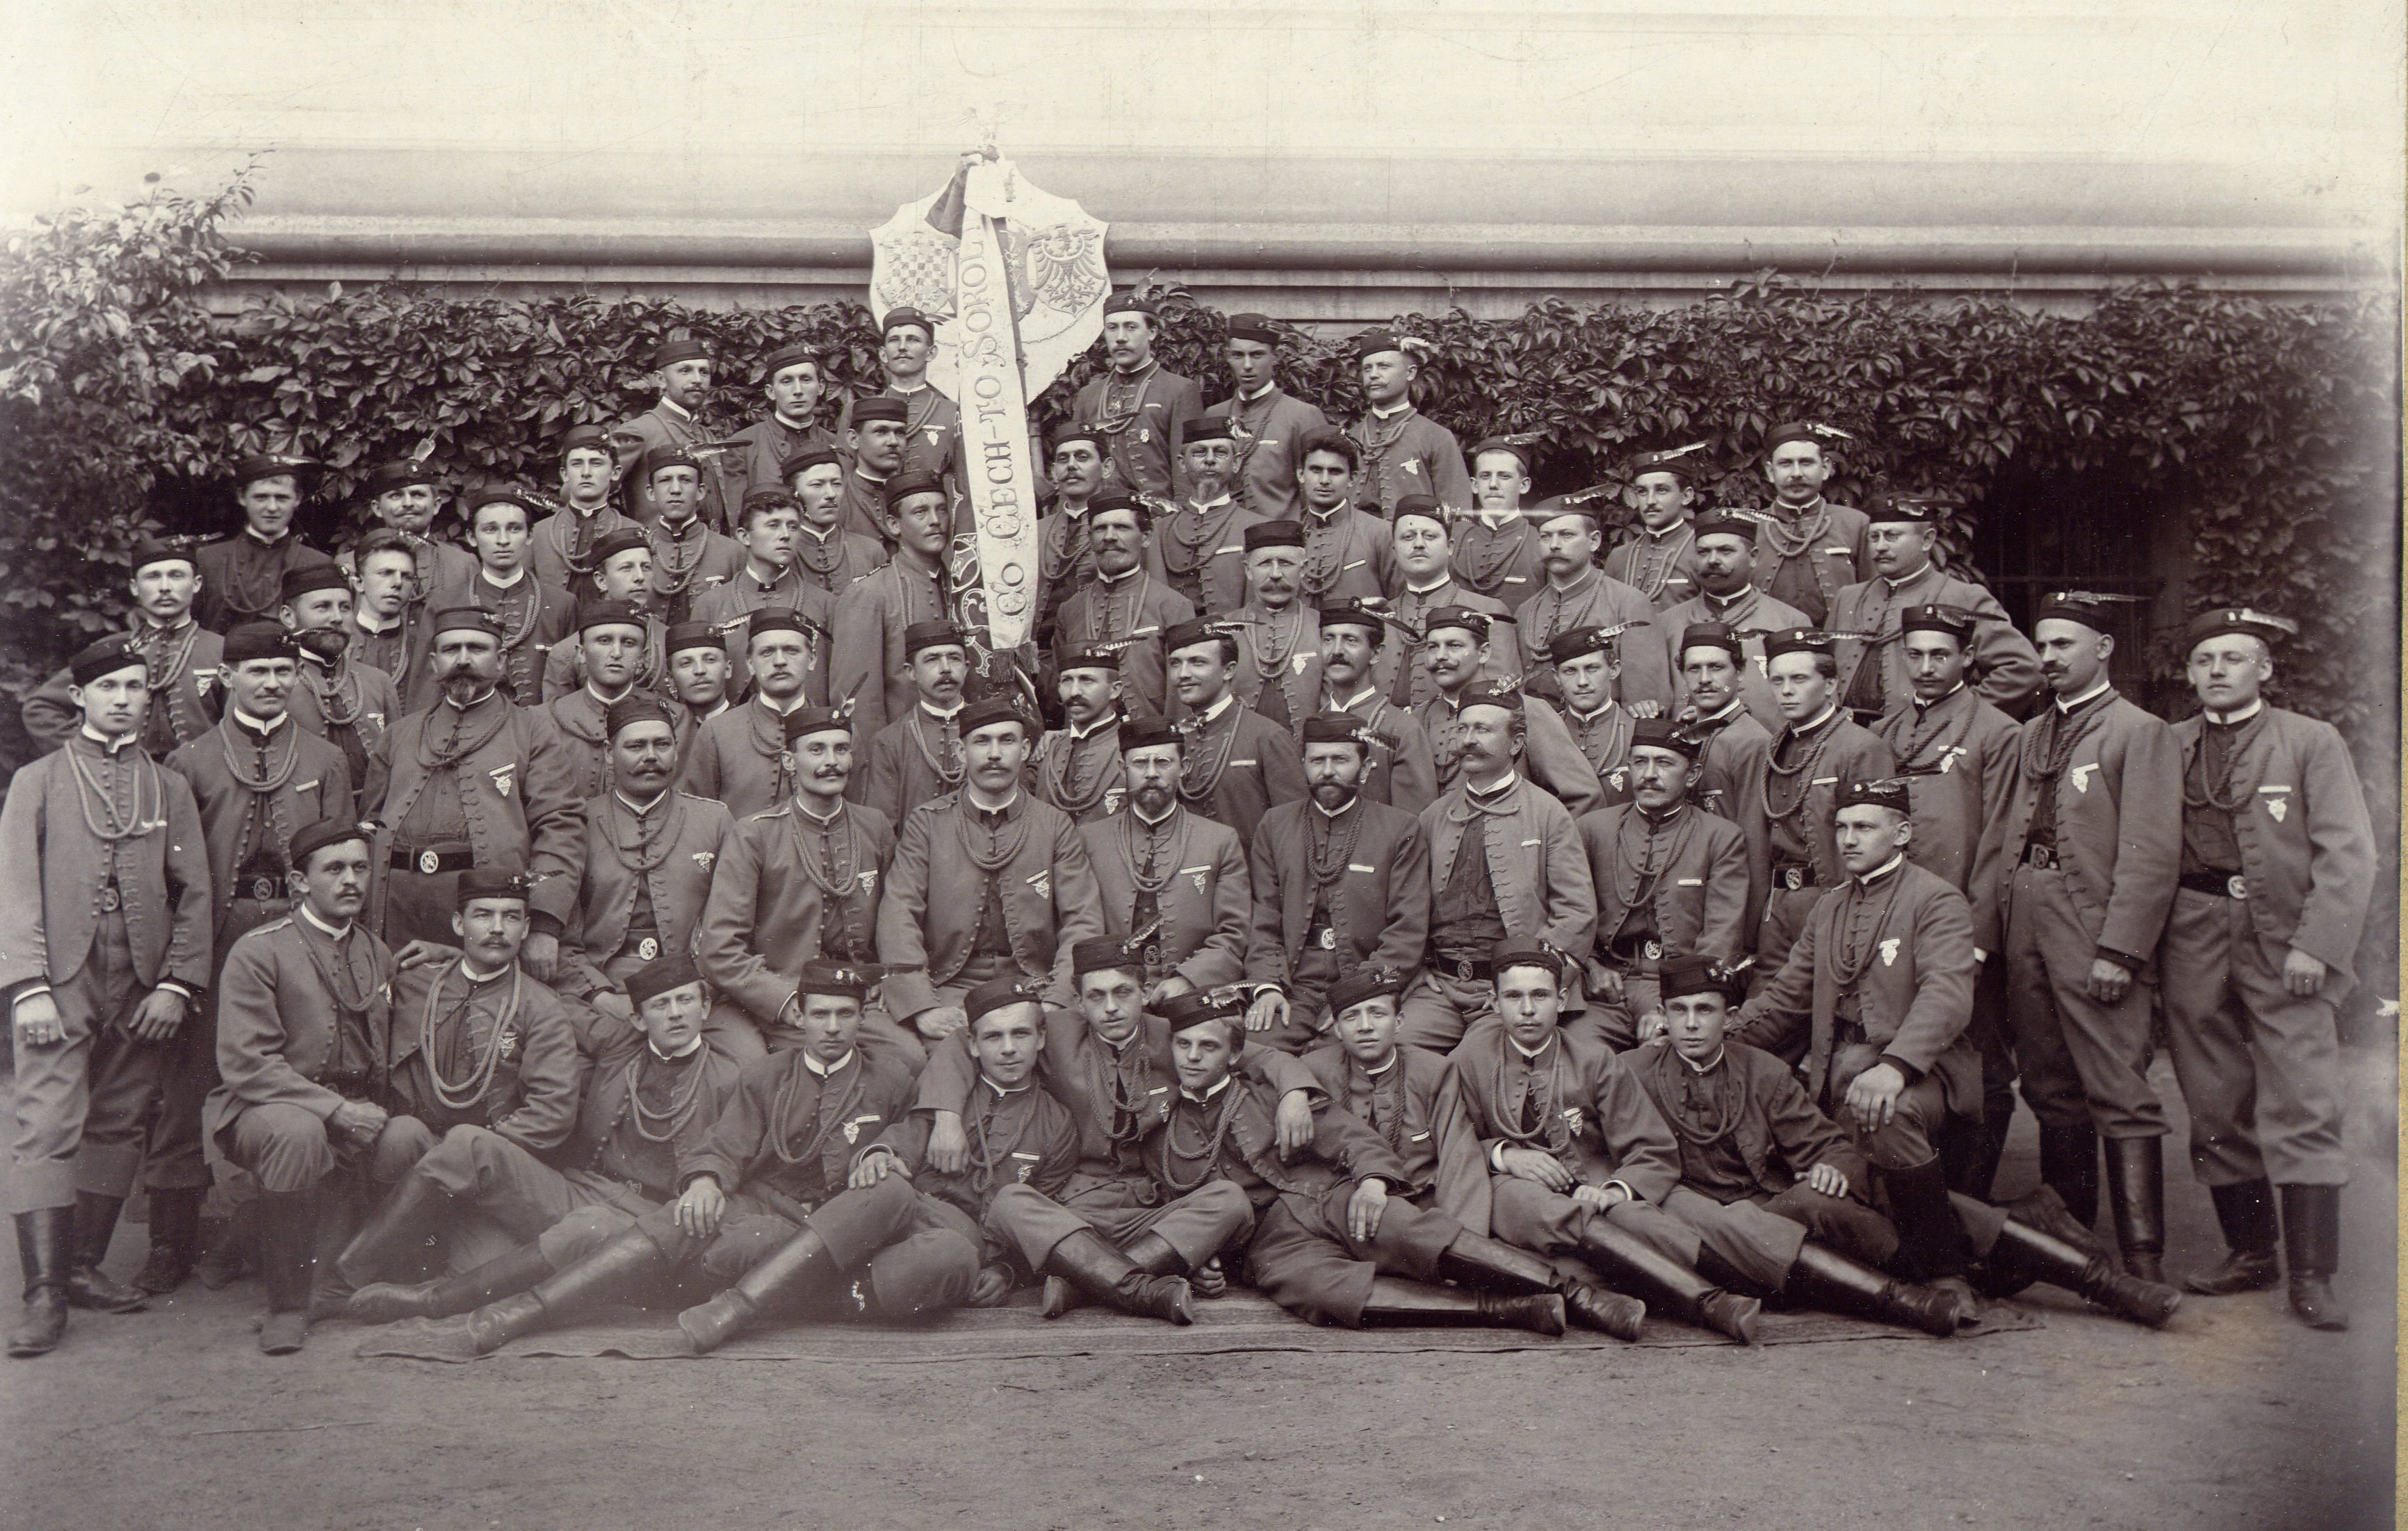
\includegraphics[width=\textwidth]{img/14_muzi_slet_1901.jpg}
  \caption*{Muži slet 1901, foto: archiv T.~J. Sokol Libeň}
\end{figure*}

\begin{figure*}[h!]
  \centering
  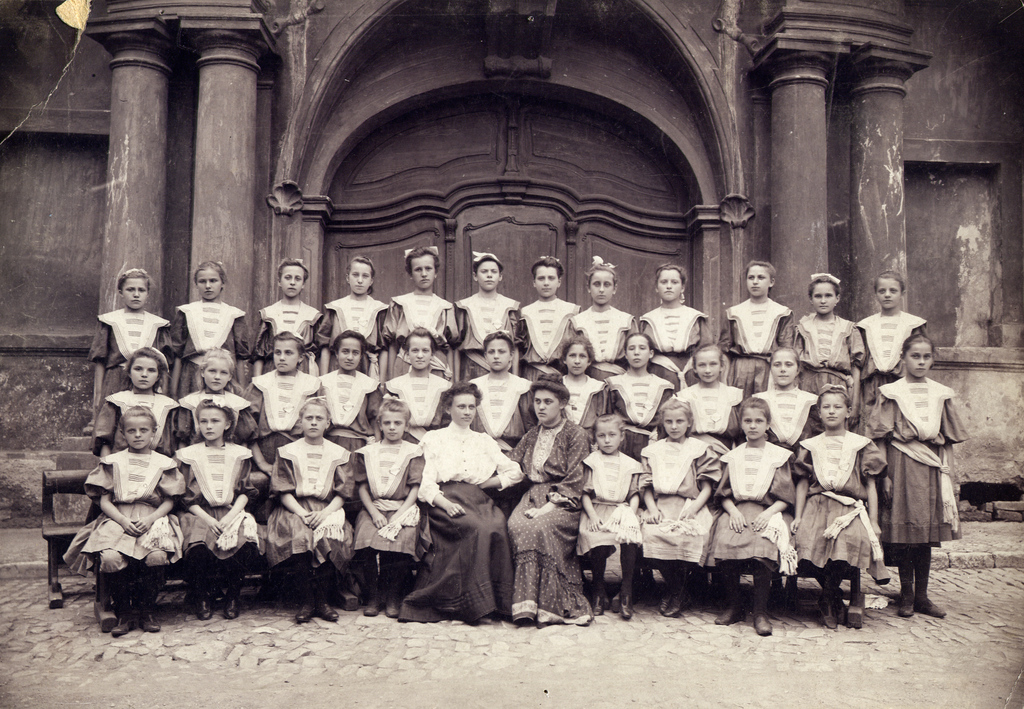
\includegraphics[width=\textwidth]{img/15_zakyne_1901.jpg}
  \caption*{Žákyně 1901, před vraty Libeňského zámku, foto: archiv T.~J. Sokol Libeň}
\end{figure*}

\begin{figure*}[h!]
  \centering
  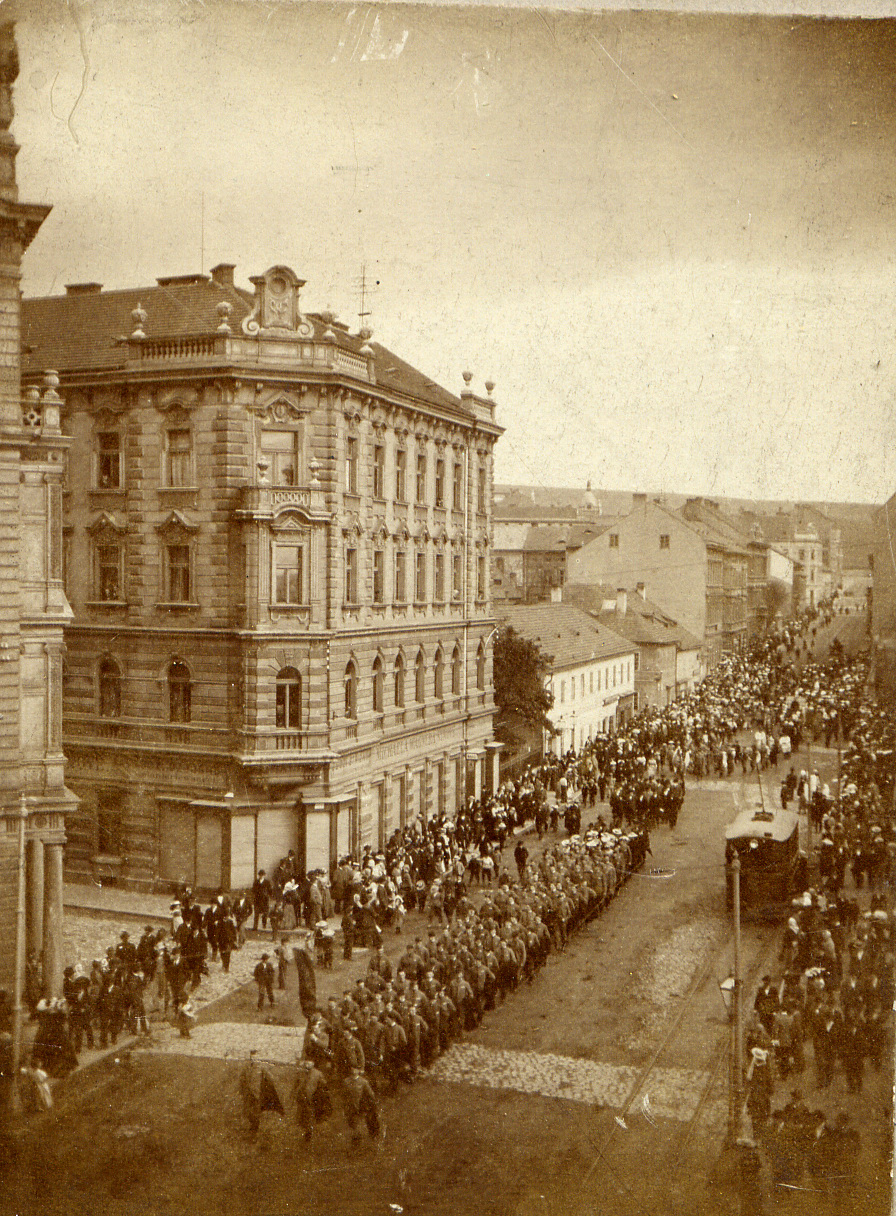
\includegraphics[width=0.8\textwidth]{img/16_pruvod_1900.jpg}
  \caption*{Sokolský průvod na dnešní Zenklově ulici při ústí Světovy ulice (vlevo). Jednopatrový bílý dům vlevo je hostinec U~Deutschů (okolo roku 1900), foto: archiv T.~J. Sokol Libeň}
\end{figure*}

\clearpage

\textbf{V. všesokolský slet (1907)} se konal potřetí na Letenské pláni, která byla znovu upravena a značně zvětšena, tribuny byly pro 55\,000 diváků. Ve společných prostných vystoupilo 7\,600 mužů. Byl to opravdu první "velký slet". V~Pamětní knize cvičitelského sboru Sokola Libeň je podepsáno pod hlavičkou V.~sletu 44 mužských účastníků s~náčelníkem Fr. Kynčlem a mnoho žen s~náčelnicí Hanou Němečkovou. Vzrůstem počtu cvičících, mužů, žen, dorostu i žactva, se od tohoto sletu začala usilovně řešit otázka výstavby sokolovny. Největší zásluhu na tom má tehdejší starosta bratr František Filip. Byl starostou od roku 1900 a byl jím až do roku 1920. Dokázal i nemožné, a tak už na oslavu dvacetipětiletého trvání jednoty byl položen 10.~října 1909 základní kámen ke stavbě sokolovny. Je zazděn ve vestibulu vedle vrátnice \pozned{(a nese v~sobě dvojici časových schránek – z~roku 1909 a z~roku 2009, pozn. ed.)}. Za 10 měsíců byla stavba dokončena a 14.~srpna 1910 otevřena.

\subsection{Výstavba sokolovny}

Čtvrtstoleté trvání Tělocvičné jednoty Sokol v~Libni nemohlo být lépe a
důstojněji oslaveno než stavbou sokolovny. Již třetí rok po založení
jednoty vznikl "Fond pro zbudování tělocvičny". Ten v~jubilejním 10.
roce (1894) vykazoval jen 2\,815 zlatých a 83 krejcarů.

Na valné hromadě 31.~ledna 1909, tedy v~roce zahájení stavby sokolovny,
činilo hotové jmění na zbudování tělocvičny 40\,872,49 K. Rozpočet na
stavbu sokolovny s~městskými lidovými lázněmi po obou stranách a
s~vnitřním zařízením zněl přibližně na 400\,000 K. Kde na to vzít? Kromě
výtěžků ze šibřinek, z~jarních a letních zábav, divadelních představení,
akademií a veřejných cvičení, tu byly jen dary organizaci a jednotlivců
a také sbírky ze šestnácti pokladniček různě umístěných, ale to byly
částky velmi malé. Například ve školní tělocvičně se vybralo za celý rok
20,94\,K., v~hostinci U~Filipů 80,18\,K., U~Bartůňků 17,69\,K., U~Jeřábků
8,10\,K. a pod.

Jaké byly tenkrát členské příspěvky? Velmi malé. Za rok 1908 (za 11
měsíců) se vybralo 1\,240,49\,K., přepočteno na jeden měsíc to je 112,70
K. To bylo od 375 dospělých a 232 mladých (dorost a žactvo). Vychází nám
tedy asi 25 haléřů na osobu měsíčně.

Za takových finančních poměrů by asi ke stavbě nedošlo, nebýt pevné vůle
celého výboru, v~jehož čele stál velmi obětavý starosta, br. František
Filip, poslanec na Sněmu Království českého, obecní starší,
velkorestauratér atd. Ten dokázal, že jednota získala na odkopávaném
svahu "Libušáku" (dnešní Horovo nám.) velmi levně pozemek. Nejprve 200
čtverečních sáhů (jeden sáh = 3,6\,m\textsuperscript{2}) po deseti
haléřích a pak ještě další část, celkem 335 čtverečních sáhů. Daleko
větší a lepší pozemek získala jednota v~místech, kde stával obecní dvůr
bývalé obce libeňské a také hasičská zbrojnice. Regulační čára však
rozdělila tento pozemek pro nás velmi nepříznivě. Opět zásluhou bratra
starosty Filipa došlo k~dohodě s~Pražskou obcí, podle níž jsme
odstoupili obci 170 čtverečních sáhů na ulici a získali 555 čtverečních
sáhů na stavbu sokolovny. To bylo v~roce 1907.

V~následujícím roce sestavila stavební komise zvolená valnou hromadou
program, co má stavba obsahovat, a člen komise br. Josef Kadlec, městský
stavitel, nakreslil několik půdorysných řešení budoucí sokolovny.
V~návrzích se již počítalo s~městskými vanovými a sprchovými lázněmi
umístěnými v~budově sokolovny, ale se samostatnými vchody. Toto řešení,
navržené a prosazené br. starostou Filipem získalo jednotě příspěvek na
tyto lázně od Pražské obce ve výši 65\,000\,K. A~mohlo se začít stavět.
Stavba byla zadána osvědčené stavební firmě Matěj Blecha z~Karlína.

\begin{figure*}[h!]
  \centering 
  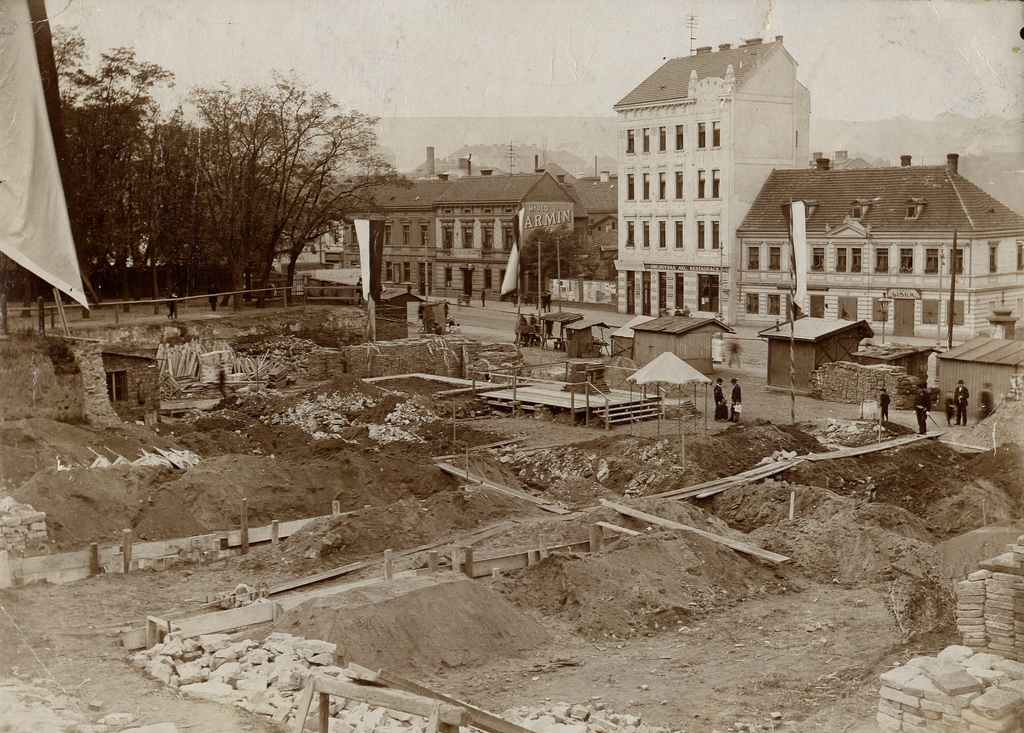
\includegraphics[width=0.9\textwidth]{img/17_zaklady_sokolovny.jpg}
  \caption*{Stavba základů libeňské sokolovny (1909), foto: archiv T.~J. Sokol
  Libeň}
\end{figure*}

Slavnost položení základního kamene se konala v~neděli 10.~října 1909.
Starosta Sokola br. Filip přivítal členstvo, dorost, žactvo i mnoho
hostů a při poklepu na základní kámen vyslovil toto přání: "Buď tvrzí
sokolstva, buď zřídlem lásky k~vlasti horoucí. Buď chrámem bratrství
ryzího nad zlato, buď ke cti nám i budoucím."

Po projevech zástupců města Prahy, ČOS, župy a mnoha jednot a dalších
hostů zakončil slavnost Zpěvácký spolek "Věnceslav" z~Libně hymnou "Kde
domov můj". Stavební firma začala kopat základy již v~pondělí 4.~října
a stavěla velmi rychle a kvalitně, takže 19.~února již bylo dosaženo
rovnosti zdiva a 19.~března byl zdvižen krov nad sokolovnou
(\pozned{sokolovna má unikátní železný nýtovaný krov nad hlavním sálem,
pozn. ed.})

\begin{figure*}[h!]
  \centering 
  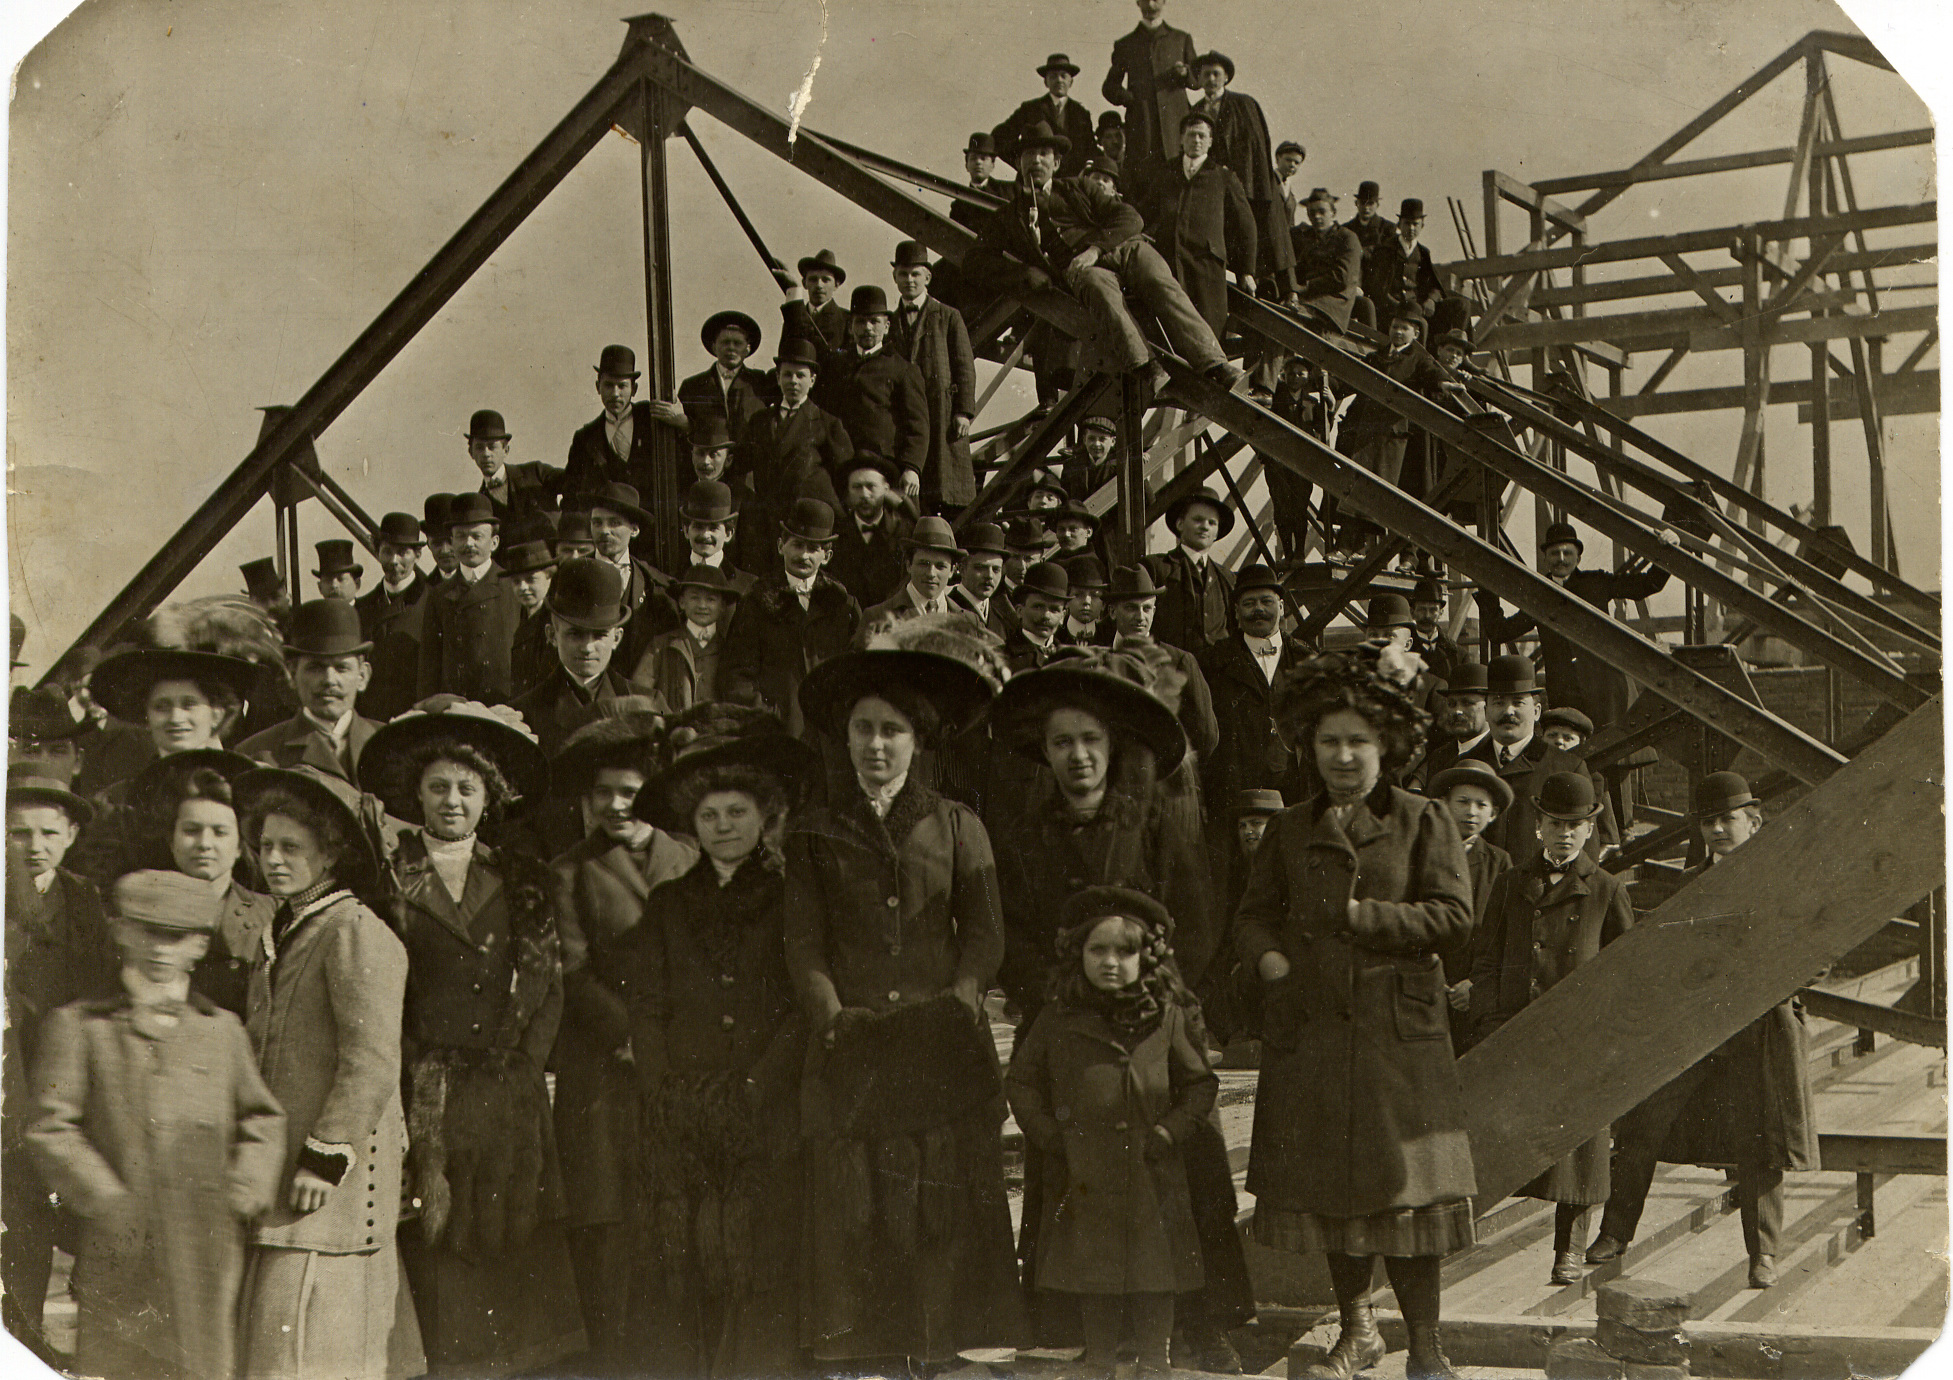
\includegraphics[width=0.9\textwidth]{img/18_krovy_sokolovny.jpg}
  \caption*{Slavnostní vztyčení krovů libeňské sokolovny (1910), foto: archiv T.~J. Sokol Libeň}
\end{figure*}

Architektonické řešení sokolovny, především hlavní průčelí, vestibul a
krásné vnitřní schodiště v~secesním slohu jsou dílem vynikajícího
architekta Emila Králíčka. Tehdy v~roce 1910 byla naše "bílá sokolovna"
skvostem vedle stejně krásného zámku a v~sousedství zajímavého kostela
sv. Vojtěcha, rovněž díla architekta Králíčka z~roku 1905. Nám se
sokolovna líbí i dnes, i když je na ní mnoho roků znát a údržba byla
dlouho zanedbávána. Nebyly peníze a nejsou ani dnes. Opravujeme kousek
po kousku, podle možností. Na generální opravu skutečně není. Asi se
zeptáte, jak to, že tenkrát dokázali tak nádhernou budovu postavit a my
ji dnes nedokážeme ani opravit? (\pozned{S odstupem 20 let od publikování
tohoto textu můžeme naštěstí částečně nesouhlasit s~tímto tvrzením --
sice krok za krokem, ale na postupné opravě sokolovny úspěšně pracujeme.
Naše nové šatny jsou toho důkazem, podobně jako nová kotelna,
rekonstrukce menších prostor, které pronajímáme, postupné opravy oken,
zrekonstruovaná sborovna, opravy dvora a zahrady sokolovny atd. Věříme
tedy, že se dožijeme dne, kdy znovu vymalujeme i velký sál a sokolovna
bude i uvnitř zářit jako nová, pozn. ed.}).

\begin{figure*}[h!]
  \centering 
  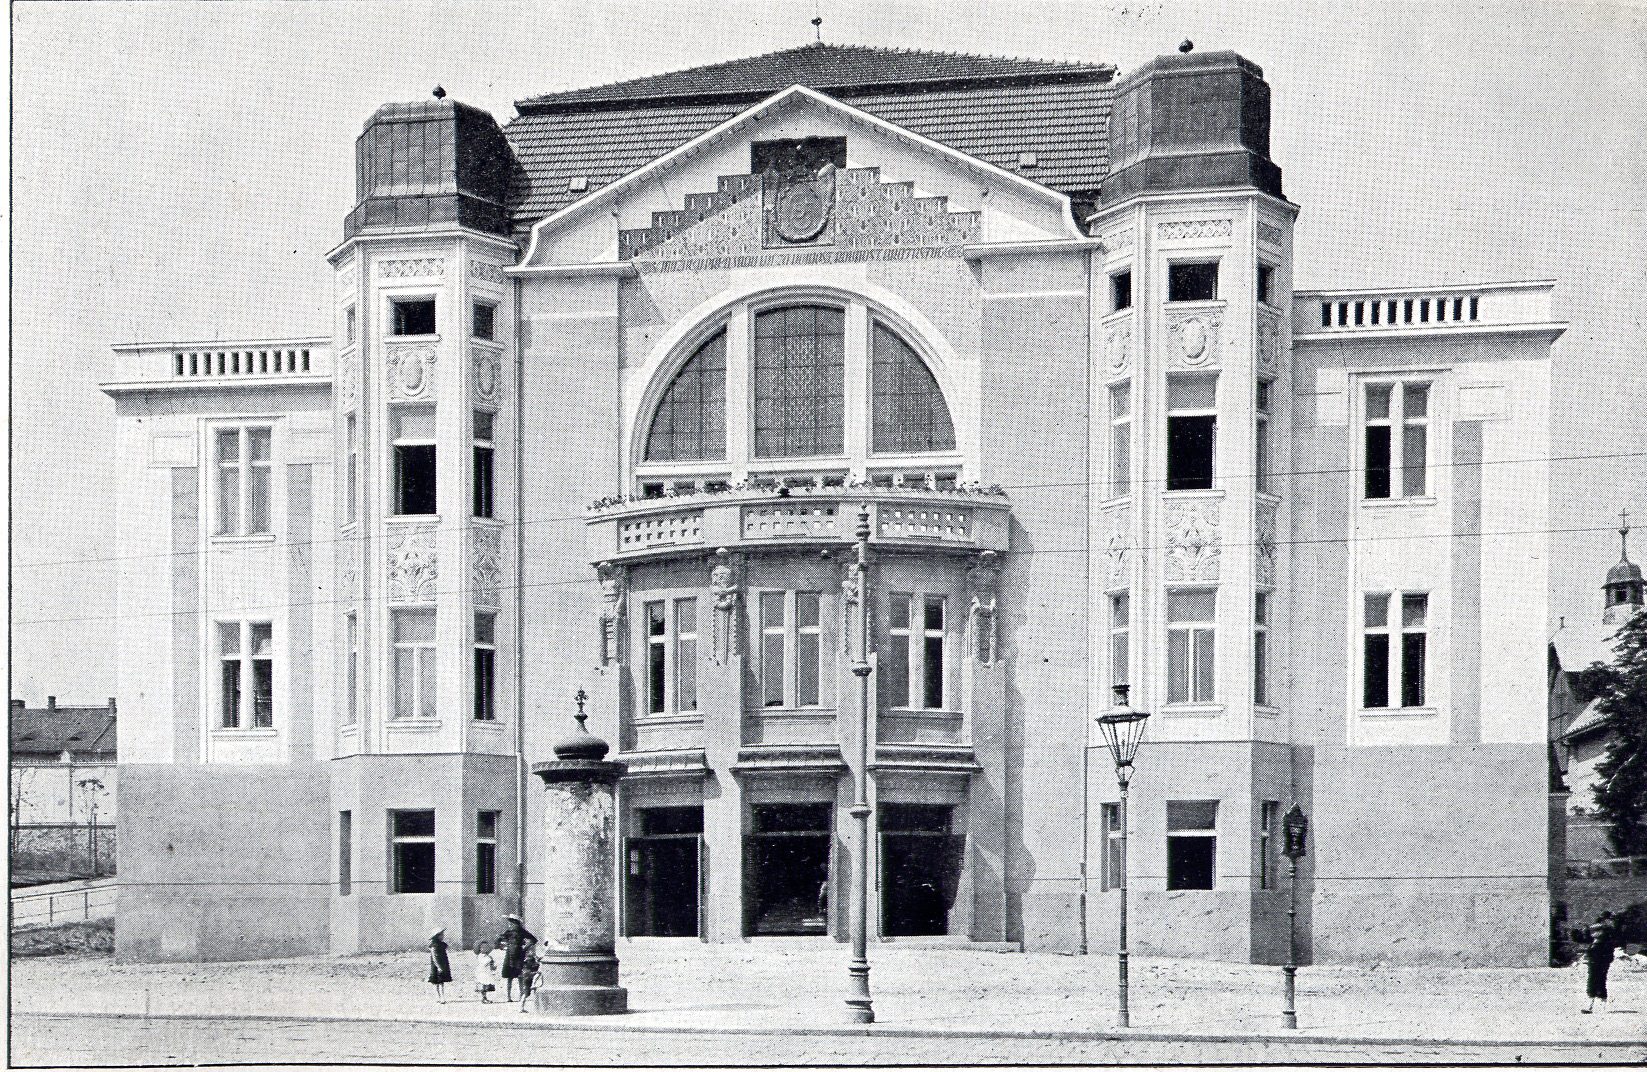
\includegraphics[width=0.9\textwidth]{img/19_sokolovna_dokoncena.jpg}
  \caption*{Sokolovna těsně po dokončení (1910), foto: archiv T.~J. Sokol
  Libeň}
\end{figure*}

Každému se naše sokolovna líbí. I~vám. Ale prohlédli jste si ji dobře?
Zastavte se opodál a sledujte s~námi a s~předsedou bývalé stavební
komise br. Josefem Holubem, stavebním radou (citujeme z~Památníku
25letého výročí Sokola v~Libni, str. 19). "Hlavní průčelí do Primátorské
třídy je obráceno na východ a bohatě zdobeno. Střed jeho, dekorativně
nejúčinnější, výstupu je segmentem před stavební čáru a jest v~dojmu
zesílen čtyřmi mohutnými pilíři, zdobenými karyatidami v~nadživotní
velikosti, jež nesou balkóny. Význam karyatid je symbolický a vztahuje
se k~předhistorickým nálezům, učiněným při odkopávce staveniště. Nad
balkónem se nalézá velké polokruhové trojdílné okno se skleněnou
barevnou mozaikou. Střed je vyvrcholen mohutným tympanonem, ozdobeným
velkým reliéfem se znakem sokolstva, a bohatými festony, jež drží
postavy sokolských borců v~nadživotní velikosti. Ostatní plocha
tympanonu jest vyplněna ornamentálními ozdobami. Po obou stranách středu
vyvinuty všemi patry probíhající mohutné pilony, jež třemi stranami
vystupují z~průčelí, tvoříce přechod k~ustupujícím postranním traktům.
Tyto pilony, jimiž se dociluje zajímavé prostorovosti hlavního průčelí,
jsou ozdobeny ornamentálními náplněmi a ukončeny osmihrannými, plechem
krytými vížkami, jež přispívají k~malebnosti střech."

\begin{figure*}[h!]
  \centering 
  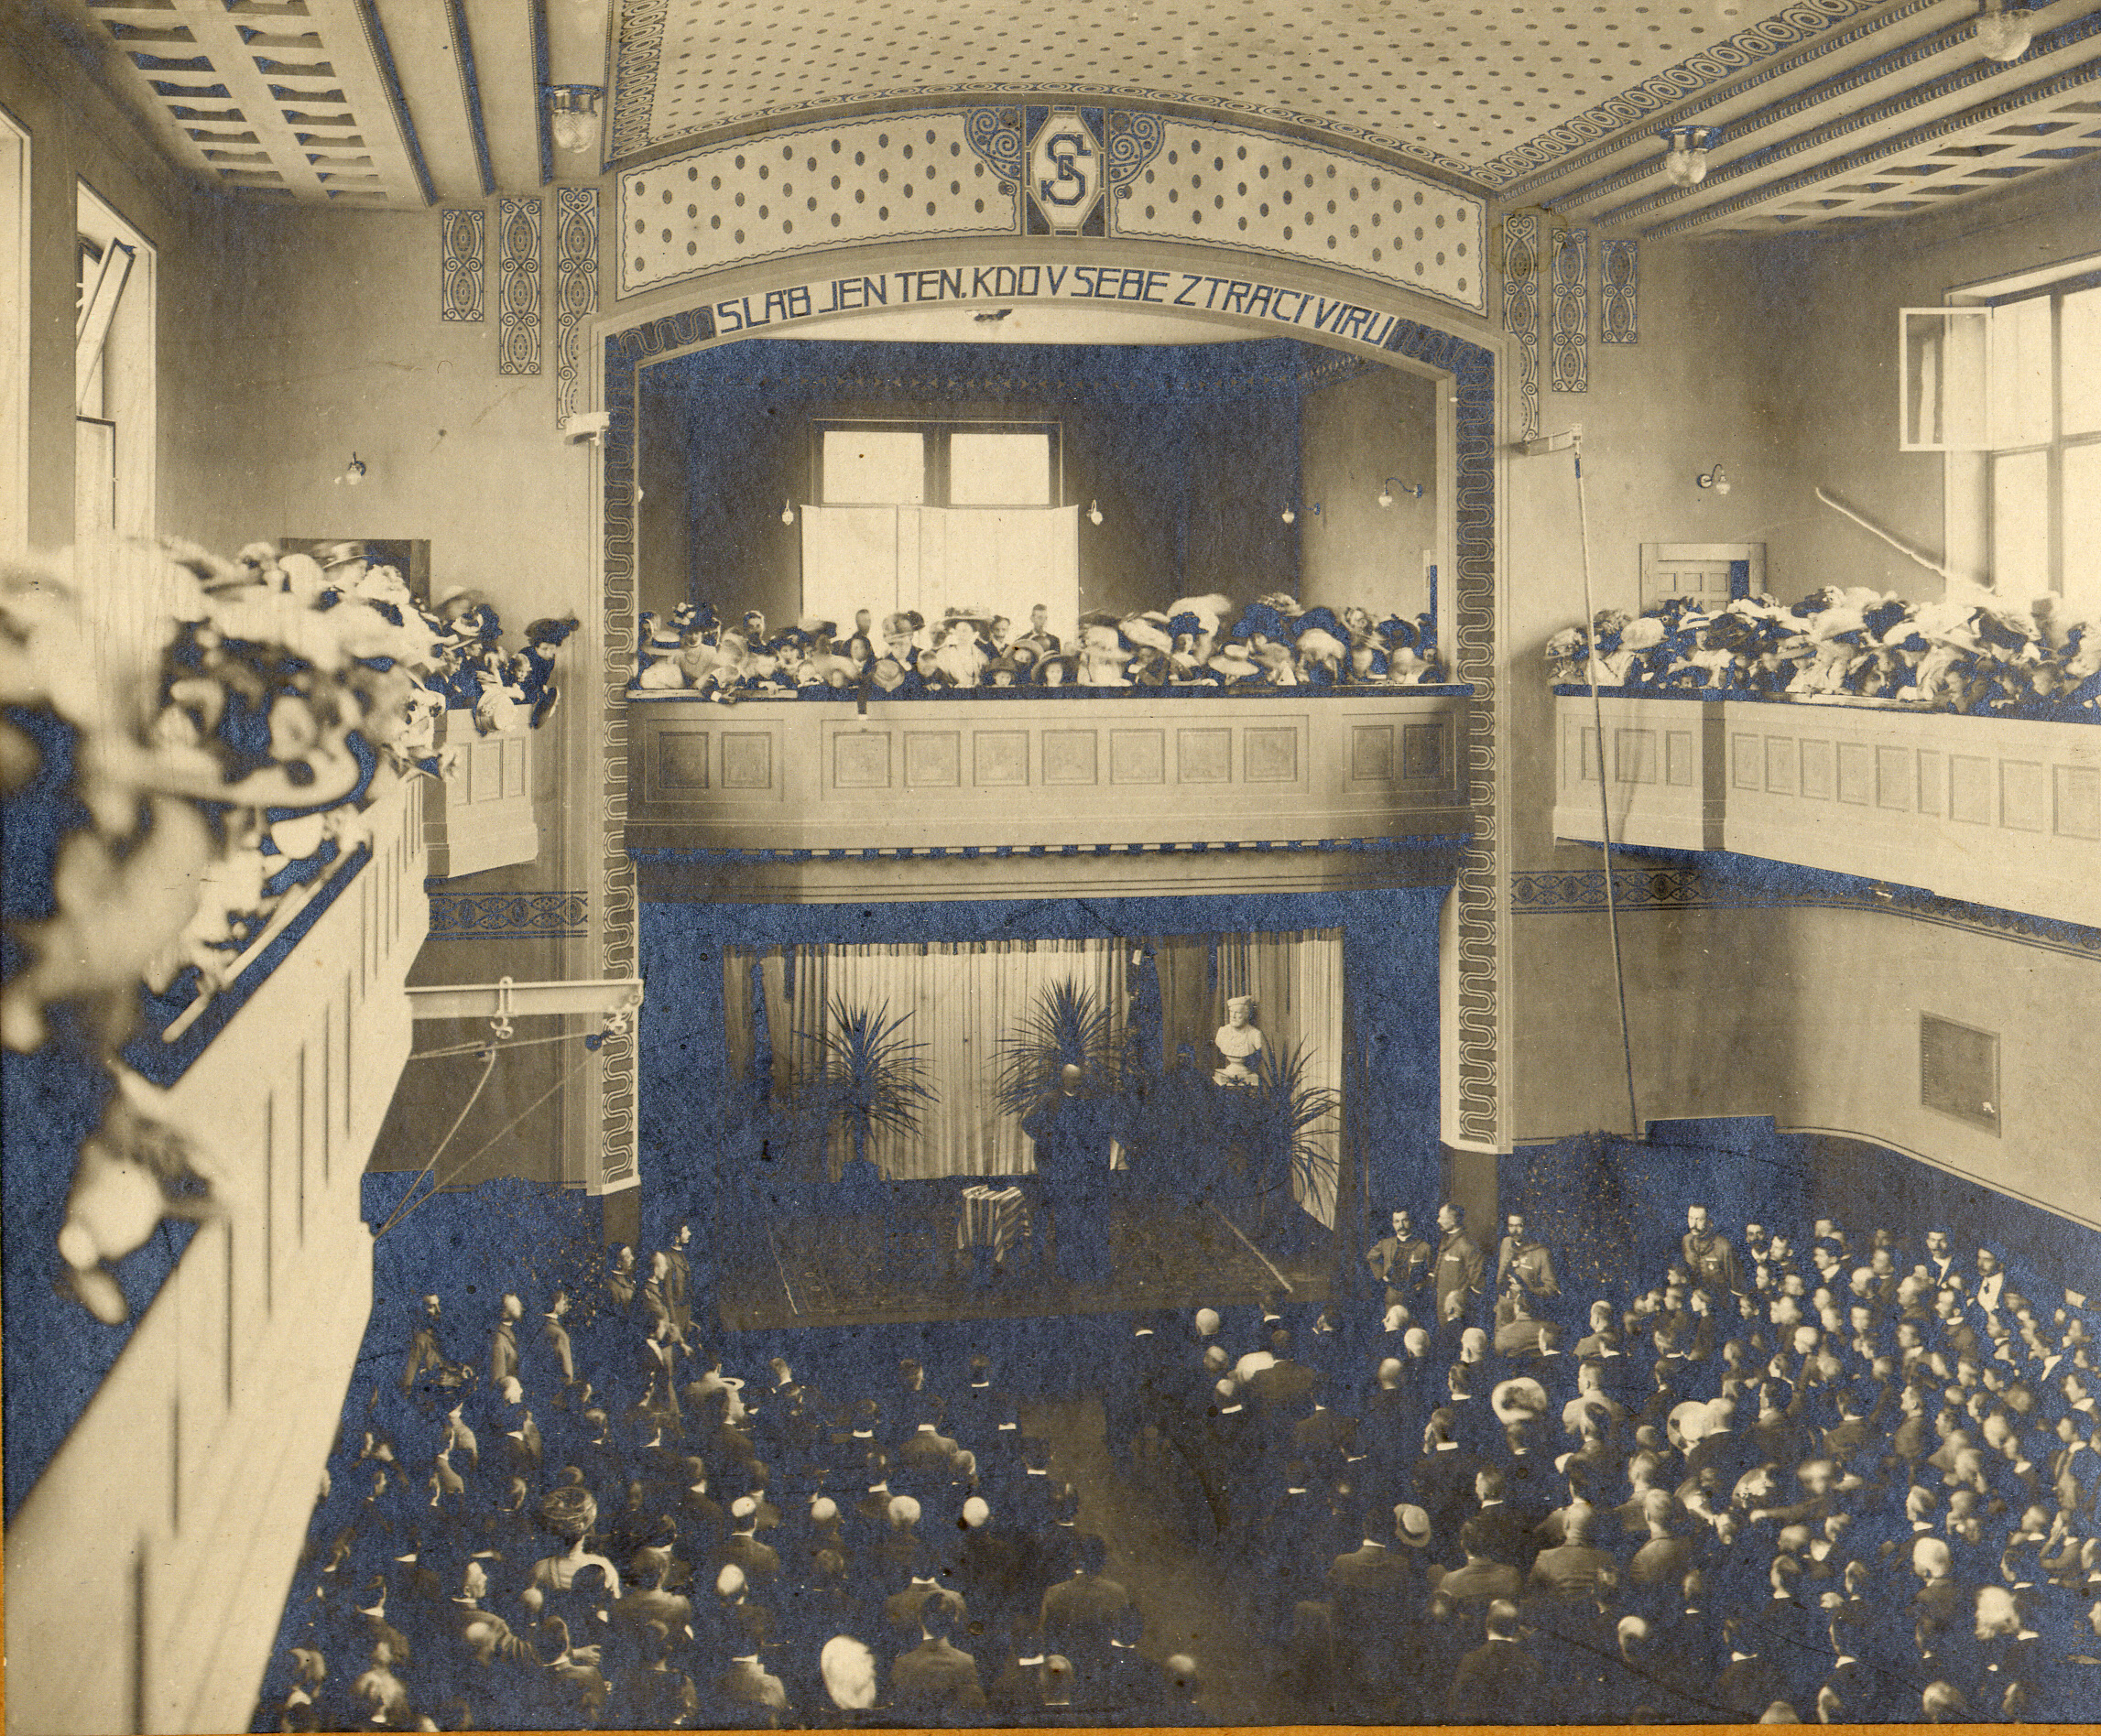
\includegraphics[width=0.9\textwidth]{img/20_velky_sal.jpg}
  \caption*{Velký sál sokolovny neznámo při jaké příležitosti, ale krátce po
  dokončení. Povšimněte si původní bohaté secesní výmalby a také oken na
  pravé galerii. Srncův sál, který je na místě dnes, byl dostavěn ve 20.
  letech, foto: archiv T.~J. Sokol Libeň}
\end{figure*}

V~tomto východním průčelí jsou tři hlavní vchody, kryté oplechovanými
markýzami. Vestibul za hlavními vchody nás vítá krásným trojramenným
schodištěm z~červeného sliveneckého mramoru. Po stranách hlavního
průčelí jsou dva přístavky. To bývaly vchody do ženských a mužských
oddělení lidových lázní. Tolik asi z~prvních informací br. Holuba. Dalo
by se ještě na mnohé upozornit, ale chceme, abyste si sami všímali a
nacházeli všechno hezké na sokolovně a našli zde svůj druhý a milý
domov.

\pozned{Několik poznámek k~zázemí sokolovny. Sokolovna byla vybavena nejen
ke cvičení, ale také k~pořádání kulturních akcí, jako byly šibřinky,
taneční zábavy a další. Proto byla v~místě dnešní klubovny turistických
oddílů v~prvním patře vpravo vzadu kuchyně a na opačné straně v~místě
dnešní posilovny výčep piva, nicméně obojí bylo v~provozu právě jen při
konání kulturních akcí, a nikoliv trvale (hospoda v~sokolovně nikdy
nebyla). Sokolovna měla zřízeno teplovzdušné vytápění sálů, jehož část
mimochodem dodnes slouží k~větrání velkého sálu. V~kotelně v~přízemí se
nacházely uhelné kotle pro ohřev vody pro lázně i vytápění, ale z~nich
byla teplá voda rozvedena pouze po přízemí. Pod hlavním schodištěm se
nachází teplosměnná komora, kde byl radiátory ohříván vzduch nasávaný
"katakombami" v~základech sokolovny a následně přiváděn do velkého
sálu, odkud dále komínovým efektem odchází průduchy ve stropě. Pozn.
ed.}

Kolik radostí přinesla členstvu, dorostu, žactvu i libeňským občanům
naše sokolovna, nelze ani vyčíslit. Velký sál, dlouhý 21,25 m a 14 m
široký, často ani nestačil přílivu nových cvičenců. Na blížící se VI.
slet se mohla jednota dobře připravit již pod vlastní střechou. V~roce
1912 měla 585 členů, z~toho 29 zakládajících, 357 přispívajících a 199
činných. Dále měla 102 členky, 49 dorostenců, 36 dorostenek, 101 žáků a
102 žákyň. Tedy celkem 975 duší (\pozned{současný počet členů jednoty je
jen o~málo nižší -- kolem 800, pozn. ed.}).

Jak byl využíván ve sletovém roce velký a malý sál, poznáme z~Výroční
zprávy za rok 1912, v~níž náčelník JUC. Václav Vávra a náčelnice Milada
Jirkovská (provdaná Vacínová) uvádějí: muži cvičili třikrát v~týdnu i
o~prázdninách, nejmenší návštěva byla 45, největší 92. Dorostenci cvičili
ve středu a v~sobotu, i o~prázdninách. Žáci v~pondělí a ve středu mimo
prázdniny. Ženám, dorostenkám i žákyním byly vyhrazeny úterky a čtvrtky.

Statistika cvičení za rok 1912:

\begin{longtable}[]{%
  >{\centering\arraybackslash}p{2cm}%
  | >{\centering\arraybackslash}p{2.5cm}%
  >{\centering\arraybackslash}p{2.5cm}%
  >{\centering\arraybackslash}p{2.5cm}}
{} & zapsáno na 1~hodině (průměr) & hodin za rok & cvičilo na 1~hodině (průměr) \\
\hline
muži & 135 & 119 & 73 \\
ženy & 31 & 87 & 25 \\
dorostenci & 54 & 85 & 31 \\
dorostenky & 18 & 87 & 14 \\
žáci & 86 & 73 & 57 \\
žákyně & 81 & 82 & 68 \\
\end{longtable}

Uvádíme statistická data proto, abychom mohli později i dnes porovnávat
zájem o~cvičení a poctivost v~docházce. Srovnáme-li poměr zařazených
s~návštěvou v~jedné hodině, vychází nám u~mužů a dorostenců návštěvnost
jen 54 \%, zatímco u~žen a dorostenek 80 \% . Žákyně byly nejpilnější,
vykazují 84 \%.

\textbf{VI. všesokolský slet (1912)} a současně I. slet slovanského
sokolstva se konal opět na Letné. Na prvním z~hlavních sletových dnů
cvičilo 92 mužů a 38 žen ze Sokola Libeň. Ve sletovém průvodu
pochodovalo 122 libeňských mužů v~krojích (pořadových cvičení v~květnu a
v~červnu se zúčastnilo asi 100 bratří; hlavně z~řad přispívajících). Ve
sletové scéně Marathón účinkovalo 13 mužů. Do sletových závodů vyslala
jednota 12 dorostenců a 13 mužů (dvě družstva a jednoho jednotlivce),
dále 3 muže do závodu prostého a 3 muže do závodu zvláštního. 1.
družstvo získalo 80,9\,\% dosažitelných bodů a přineslo lipový věnec se
stříbrným odznakem a velký diplom. Vítěz získal 93\,\% bodů. Dobře si
vedlo i druhé družstvo (malý diplom) i ostatní závodníci. Např. br. Boh.
Vágner byl ve skoku o~tyči třetí výkonem 2,80\,m. Členové jednoty
pracovali i v~několika sletových odborech a na sletových závodech jako
rozhodčí. Pro účastníky sletu z~naší pohraniční svěřenky v~Kopistech
u~Mostu uspořádali v~sokolovně přátelský večer, opatřili noclehy a dělali
jim průvodce po Praze.

Radostný a velmi čilý byl život jednoty v~nové tělocvičně, ale ne na
dlouho. V~roce 1914 vypukla 1. světová válka. Naše nová sokolovna se
proměnila ve vojenský lazaret. Hodně mužů narukovalo, pro dorostence
zajistil náčelník se starostou cvičení v~"Libušině škole". Oblíbený
vedoucí dorostenců br. Vaniš narukoval, velení převzal br. Jan Koubek.
Osvědčil se stejně dobře a tak na župních závodech v~roce 1918 se naši
dorostenci umístili na prvním místě. Sokol ve válečných letech vlastně
neexistoval. V~květnu 1915 byl zatčen a uvězněn starosta ČOS br.
Scheiner a v~listopadu 1915 byla rozpuštěna ČOS i Svaz slovanského
sokolstva.

\begin{figure*}[h!]
  \centering 
  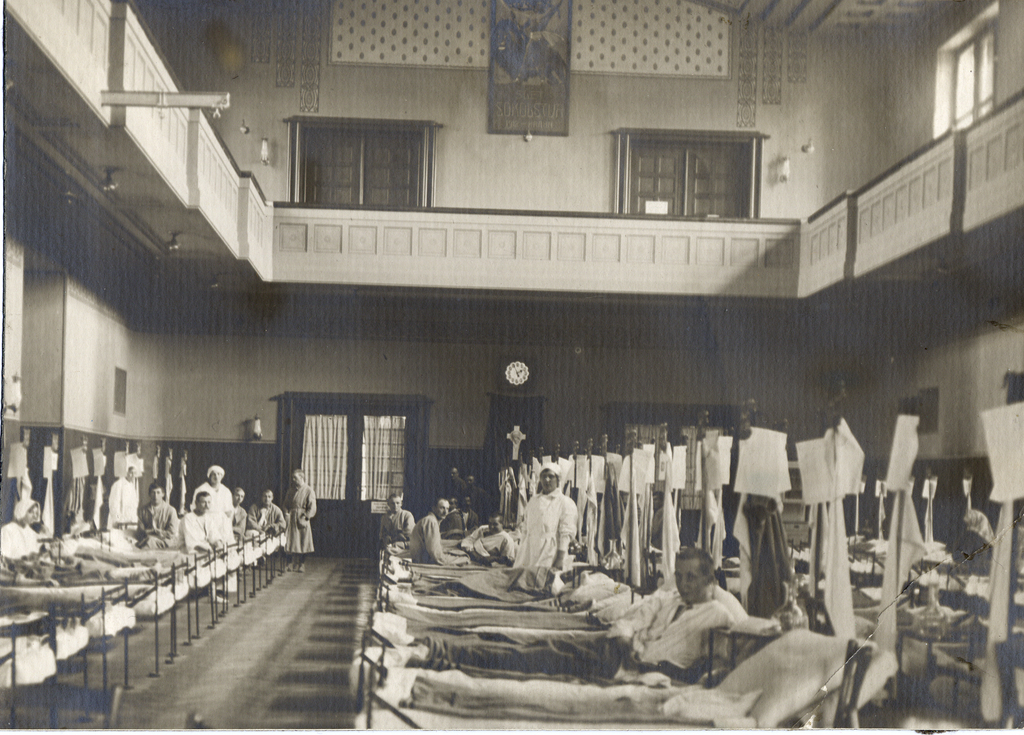
\includegraphics[width=0.9\textwidth]{img/22_lazaret.jpg}
  \caption*{Velký sál sokolovny jako lazaret (1917), foto: archiv T.~J. Sokol
  Libeň}
\end{figure*}

Ve vojenském lazaretu v~sokolovně pomáhaly naše členky šitím prádla a
ošetřováním raněných. Ke cvičení byla sokolovna uvolněna až začátkem
února 1919.

\begin{figure*}[h!]
  \centering 
  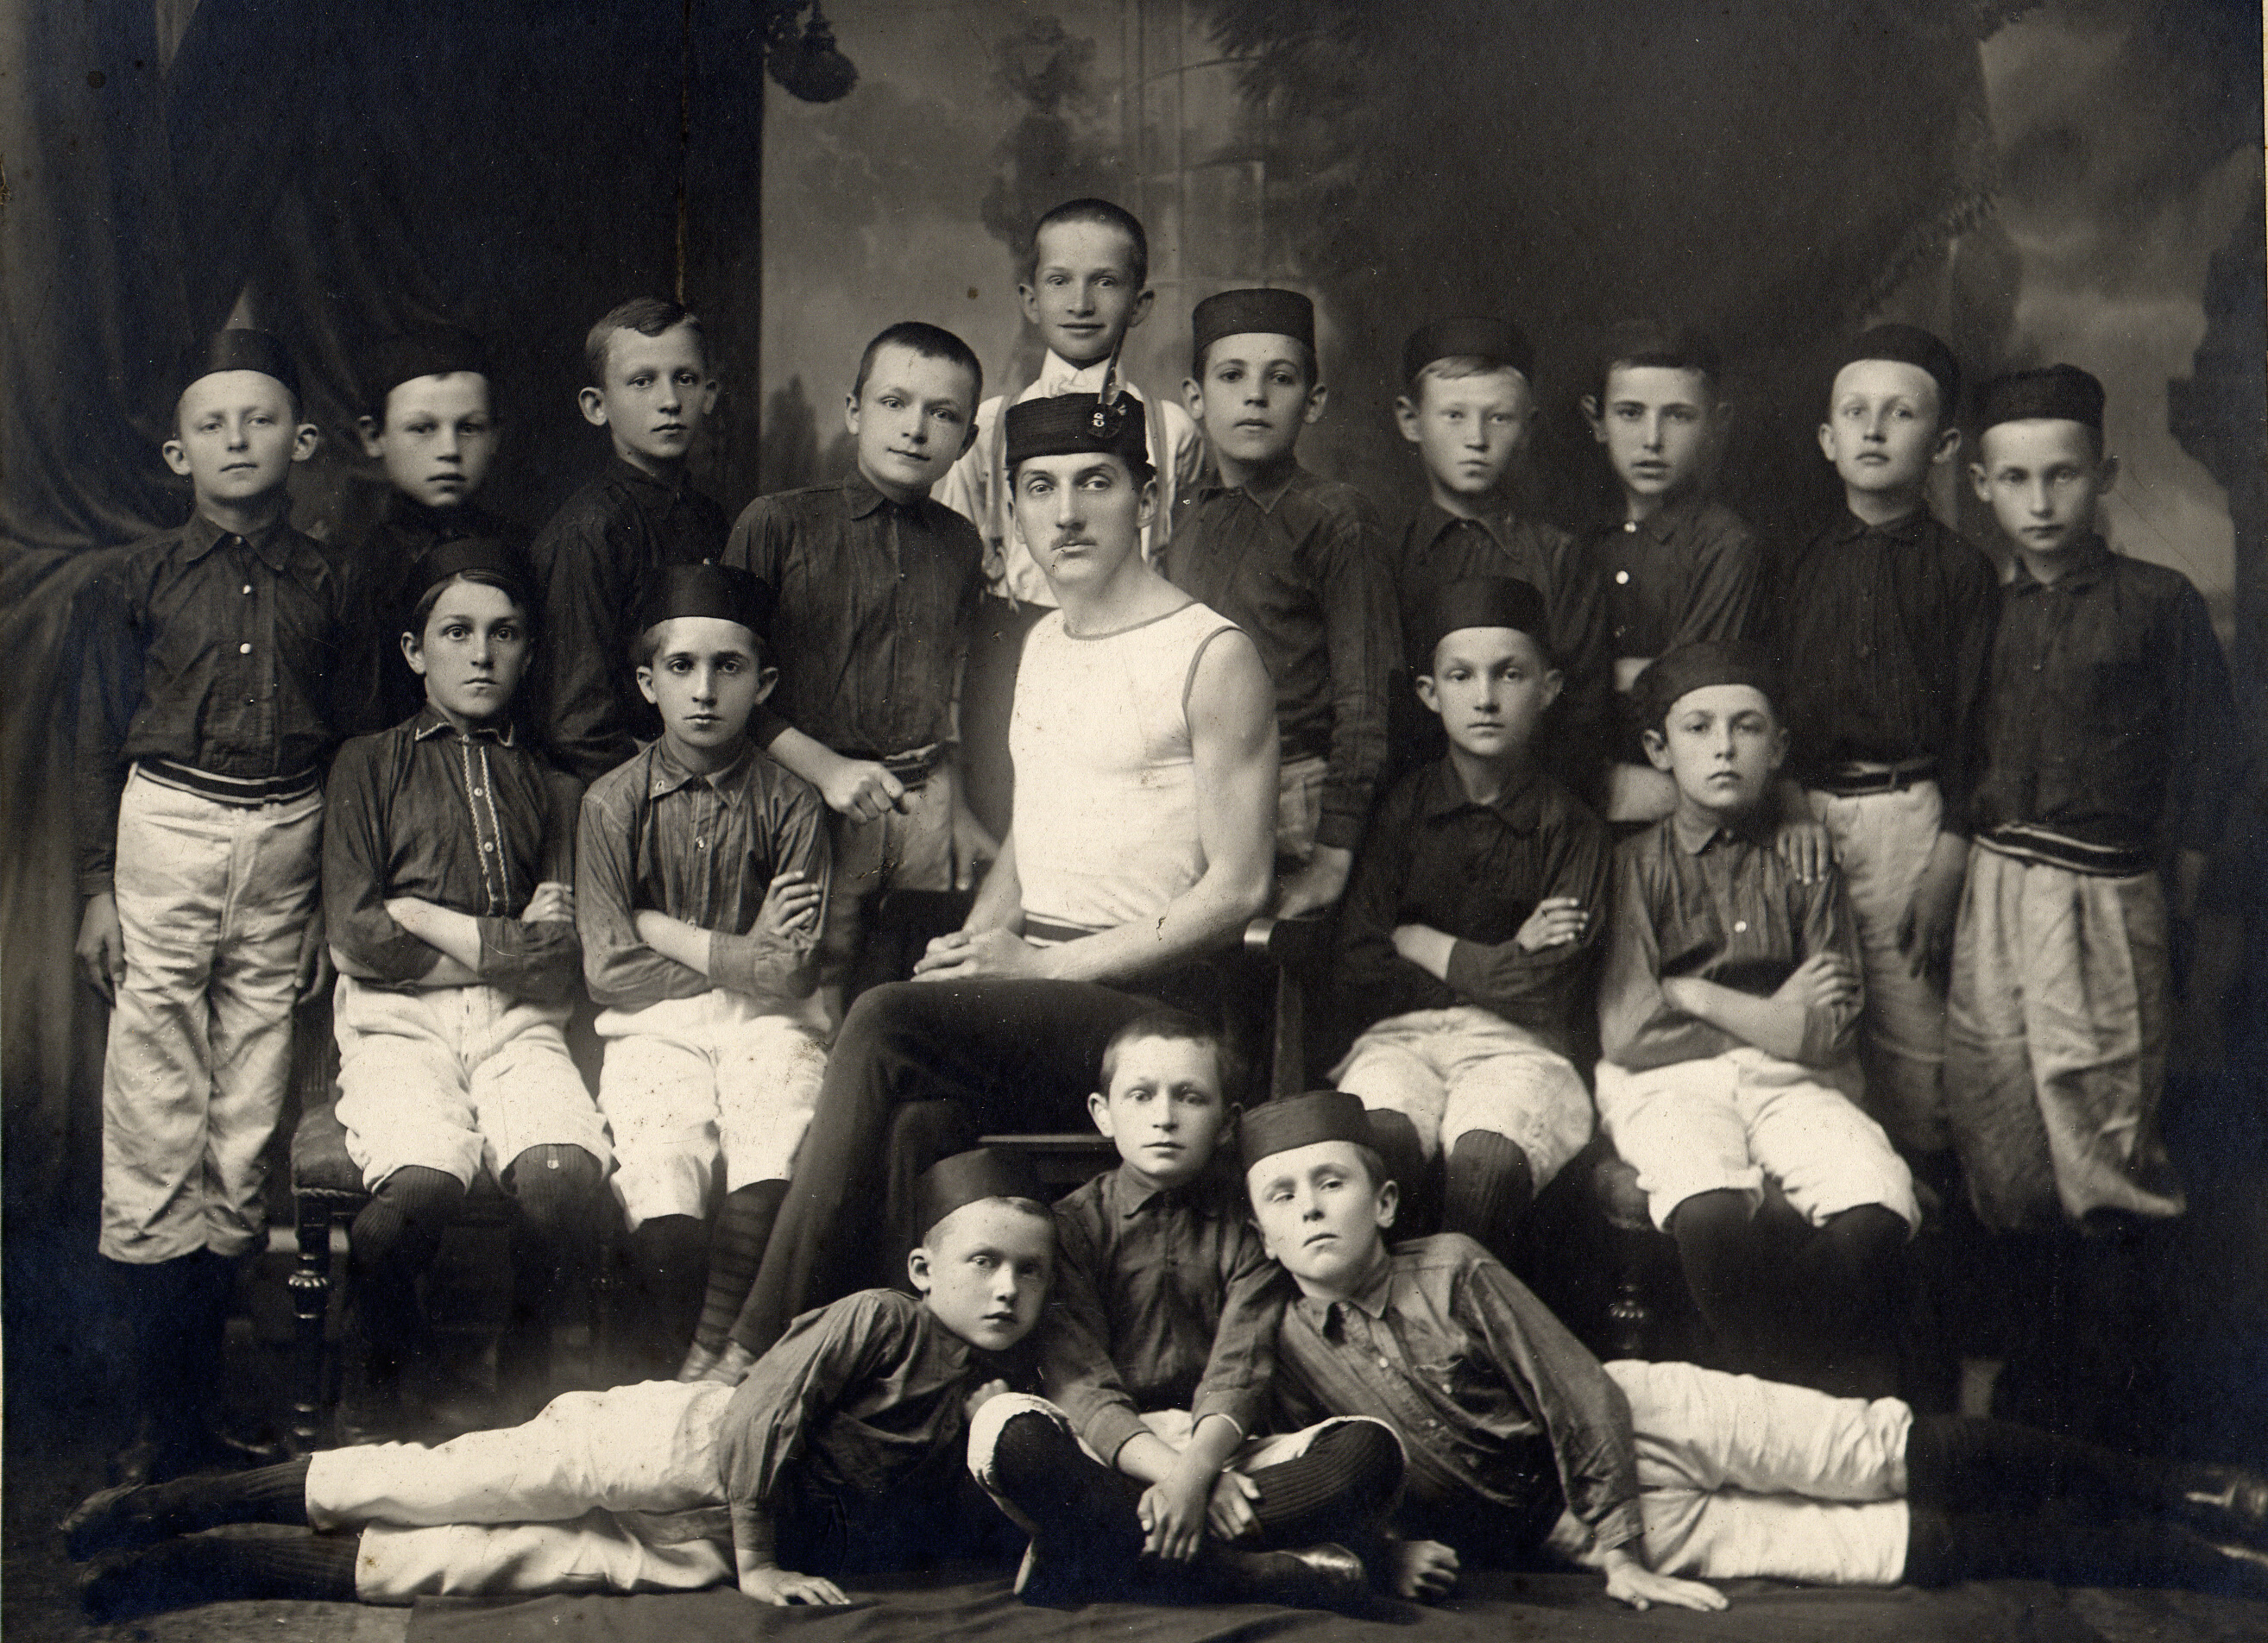
\includegraphics[width=0.9\textwidth]{img/21_zaci_1916.jpg}
  \caption*{Fotografie družstva žáků; datována 1916, ale s~ohledem na průběh
  války může být o~nějaký rok mladší či starší; foto: archiv T.~J.
  Sokol Libeň}
\end{figure*}

\textbf{VII. všesokolský slet (1920)} na Letné.

Bylo to velmi smělé rozhodnutí ČOS konati slet tak krátce po ukončení 1.
světové války a nedlouho po vzniku Československé republiky 28.~října
1918. Avšak nadšení bylo veliké a překonávalo všechny překážky. Na
Letenské pláni cvičilo čtyřikrát víc cvičenců než na VI. sletu v~roce
1912. Pro představu -- z~Libně vystoupilo na sletě 300 žáků
(\pozned{skladba žáků z~toho sletu byla rekonstruována a zacvičena
u~příležitost 120. výročí založení naší jednoty v~roce 2004, pozn. ed.}).

I~libeňská jednota zaznamenala obrovský přírůstek členstva a mládeže.
Průměrná návštěva v~jedné cvičební hodině byla ve sletovém roce 1920
tato: 111 mužů a 115 žen, 160 dorostenců a 170 dorostenek, 388 žáků a
305 žákyň. Nejsou to čísla vymyšlená, odpovídají přibližně čtyřnásobku
hodnot z~roku 1912. Podrobnosti můžeme doložit v~našich Zprávách z~roku
1930, str. 46 až 48 (\pozned{dochovány v~archivu, pozn. ed.}), kde je i
grafický diagram celého desetiletí.

\begin{figure*}[h!]
  \centering 
  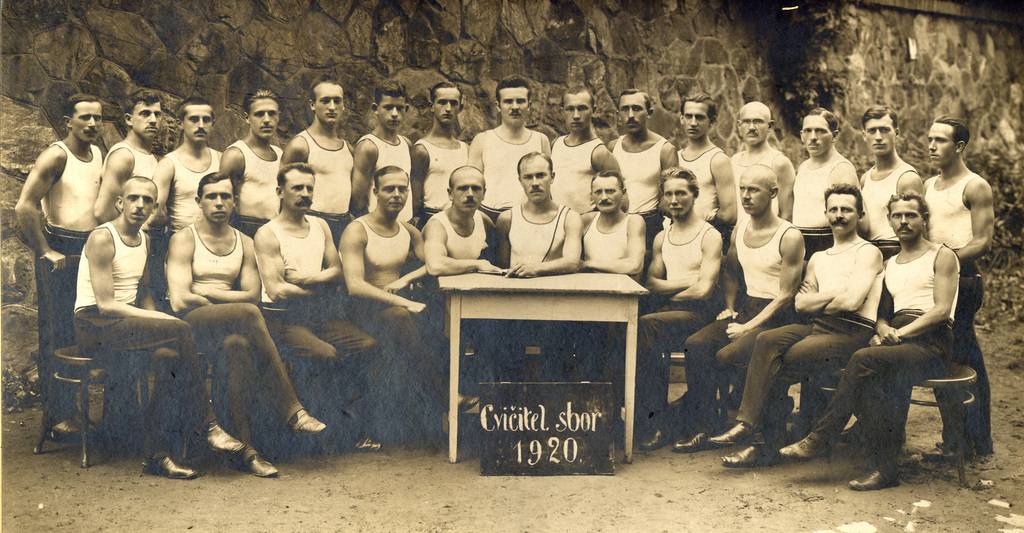
\includegraphics[width=0.9\textwidth]{img/23_muzi_cvicitele.jpg}
  \caption*{Cvičitelský sbor mužů 1920, foto: archiv T.~J. Sokol Libeň}
\end{figure*}

\begin{figure*}[h!]
  \centering 
  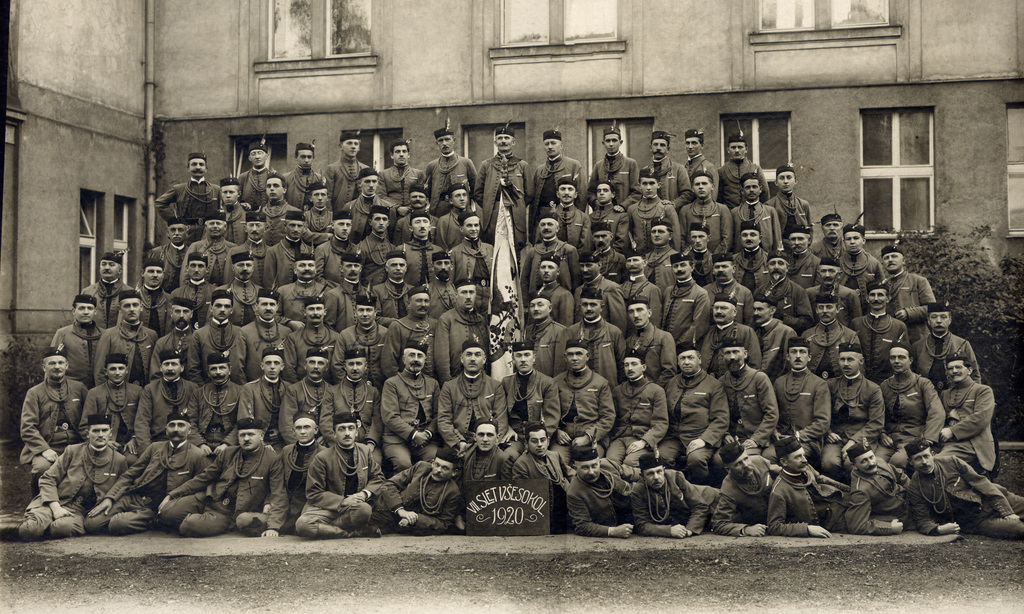
\includegraphics[width=0.9\textwidth]{img/24_muzi_slet.jpg}
  \caption*{Muži 1920 s~praporem jednoty, fotografování u~příležitosti VII. všesokolského sletu, foto: archiv T.~J. Sokol Libeň}
\end{figure*}


\section{Činnost libeňských sokolů před II. světovou
válkou}

Cvičitelé ani sokolští činovníci to neměli v~těch dvacátých letech, po
první světové válce, lehké. Členstva, dorostu i žactva stále přibývalo a
tělocvičné sály v~sokolovně nestačily. Od roku 1921 se cvičilo také ve
školních tělocvičnách v~gymnáziu, v~chlapecké škole proti zámku a
v~dívčí škole "Libušině". Správní výbor se rozhodl přistavět další sál
nad pravou lodí sokolovny (dnešní Srncův sál). Byla vypsána půjčka na 5
let. Od 465 členů, dorostu i žactva se vybralo 98\,000\,Kč (zaokrouhleno).
Dary od 558 členů vynesly 45\,000\,Kč. S~přístavbou se v~létě začalo a za
půl roku se sál za 163\,000\,Kč již používal. Tak rychle a dobře pracoval
tehdejší výbor. Starostou byl JUDr. Norbert Zavadil, jednatelem Ludvík
Schötter, dobrovolný, neplacený činovník, který např. v~roce 1922
vykazoval 2\,960 dopisů přijatých a odeslaných (mimo pozvánky na schůze,
na sokolské sliby apod.). Dělme to 365 a vyjde nám na den 8 dopisů --
při 17 řádných schůzích výboru za rok to znamená vybrat to
nejdůležitější ze 174 dopisů pro jednu schůzi. A~přece se všechno stihlo
-- nebyla televize! (\pozned{Pablo Picasso: Dnešní mládež je hrozná;
nejhorší je, že už k~ní nepatříme, pozn. ed.})

Cvičitelský sbor mužů měl od roku 1922 nového náčelníka Vojtu Vacína
(zemřel roku 1942 v~koncentračním táboře). Staral se zkvalitňování
cvičitelského sboru, stejně jako dřívější náčelníci. Po každém
pravidelném cvičení mužů -- třikrát v~týdnu -- byla půlhodinka
cvičitelského sboru. Stejně nutná byla účast cvičitelů na měsíčních
schůzích. Všechno nové v~tělovýchově se rychle zavádělo i v~Libni. Např.
cvičení a pobyt v~přírodě a hlavně prostý tělocvik (atletika) a hry.
V~roce 1921 zakoupil výbor 8 amerických stanů, míče a tábornické potřeby a
už se konalo první táboření 22 žáků celý týden na Moravě v~okolí
Macochy. O~rok později trávilo žactvo několik prázdninových týdnů
s~bratrem Malým (tatínek Marie Kodlové) a dalšími cvičiteli v~hájovně "Na
kopě" u~Kostelce nad Labem. Příští rok to byly Soutice u~Vlašimi, kde
po 4 týdny si 46 dětí užívalo hezké prázdniny opět pod vedením bratra
Malého. Žákyním poskytla ubytování liběchovská sokolovna. Vedoucími byly
sestry Decastellová starší a Kleinová. Prázdninové osady se tak vžily,
že se každý rok opakovaly.

O~koupání ve Vltavě a výcvik v~plavání se staral cvičitelský sbor. Výbor
si pronajal na libeňském ostrově tzv. Špičku s~přístupem přívozem za
ústím Rokytky do Vltavy. Mnozí ještě dnes vzpomínají, jaké to tam bylo
pěkné. Tehdy Vltava nebyla ještě regulovaná, voda v~ní byla čistější a
nebyla tak studená jako dnes.

\subsection{Budování letního
cvičiště}

Ve dvacátých letech vzrostl všude zájem o~prostý tělocvik a hlavně
o~hry. Cvičitelský sbor vedený náčelníkem Vacínem podal výboru návrh na
zajištění pozemku a zřízení letního cvičiště na svahu pod zámeckým
vrchem. Část pozemku tehdy patřila Pražské obci a byla nám pronajata
bezplatně. Druhá část byla majetkem továrny Grab a synové, pozemek
jednotě pronajala. Na tak důležitý podnik bylo třeba svolat mimořádnou
valnou hromadu. Ta však nepochopila důležitost letního cvičiště, zalekla
se nákladu, povinné členské daně i pracovních povinností a návrh
neschválila. Souhlasila však s~tím, že cvičitelské sbory provedou
potřebné odkopávky i přemístění zeminy (přes 4\,000 m\textsuperscript{3})
zdarma a že se za pomoci věrných starších členů postarají také o~úhradu
nutných nákladů. Byl to velký a těžký úkol, před kterým couvla valná
hromada jménem 1\,875 dospělých mužů a žen. Byla to osobnost Vojty
Vacína, která strhla do práce všechny cvičící i s~dorostem, a byl to
bratr Karel Besser, náměstek starosty, který se stal prvním předsedou
"Staré gardy", založené 25.~července 1923, která dokázala pokrýt
všechny výdaje s~letním cvičištěm. Byli to ti Sokolu nejvěrnější.

\begin{figure*}[h!]
  \centering 
  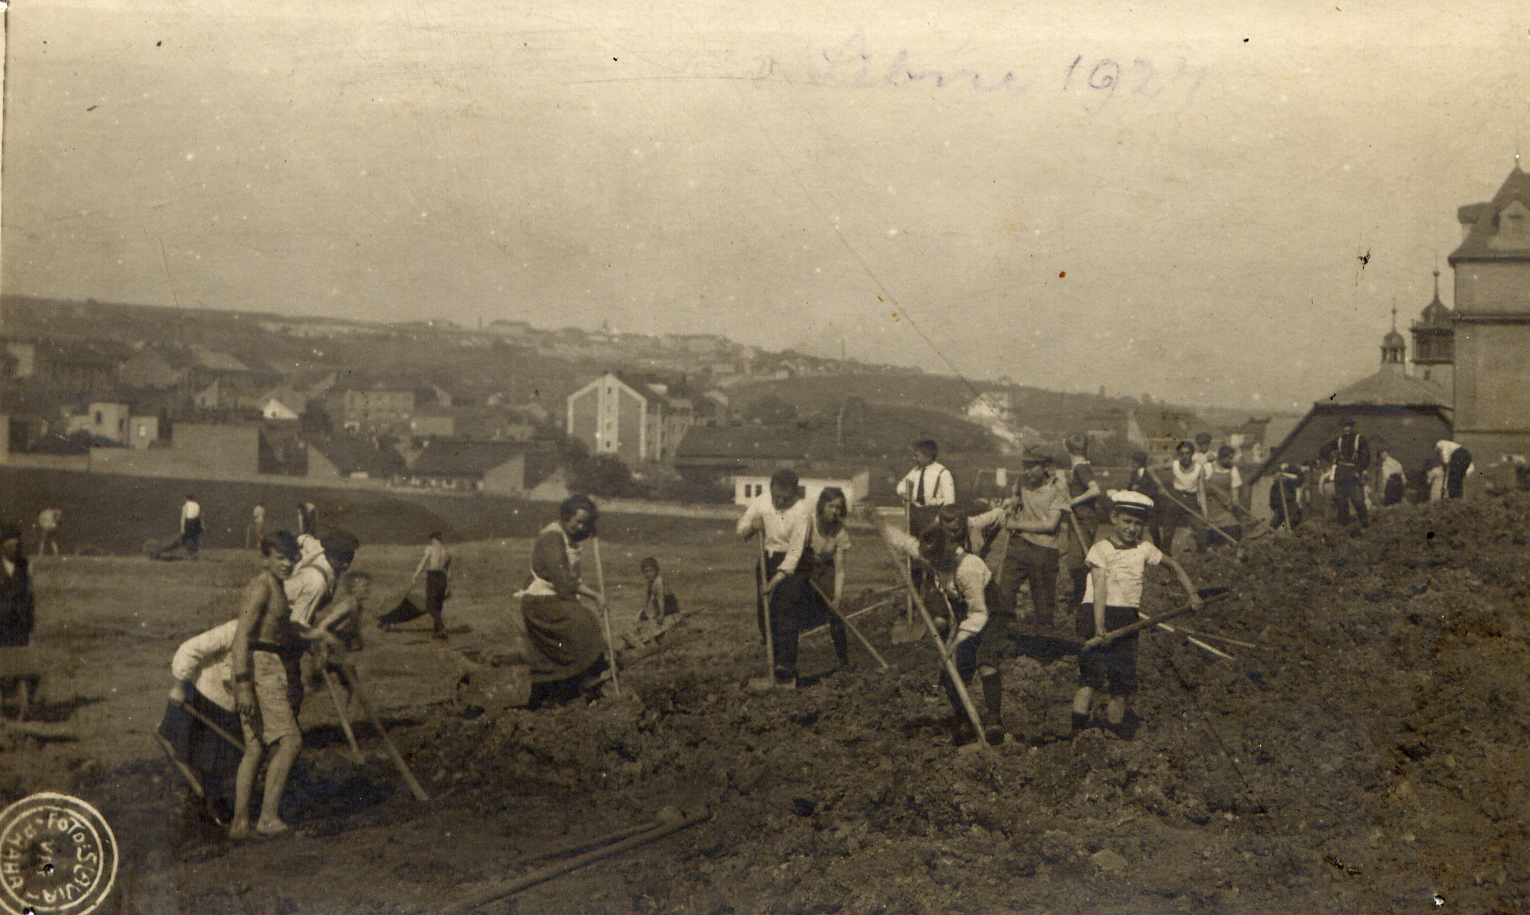
\includegraphics[width=0.9\textwidth]{img/25_budovani_cviciste.jpg}
  \caption*{Budování letního cvičiště (1924), foto: archiv T.~J. Sokol Libeň}
\end{figure*}

V~neděli 6.~května 1923 se začalo rodit naše letní cvičiště. Krumpáče,
lopaty a kolečka, všechno vypůjčené a všeho málo; alespoň ty první týdny
a měsíce. Nadšení bylo veliké. Muži odpracovali 12\,452 hodiny,
nejpilnější byl bratr František Pek, odpracoval 462 hodiny. Pomáhalo i
175 žen; 193 dorostenců a dorostenek a všichni dohromady odpracovali 16
764 hodiny. Konečnou planýrku prováděli odborní dělníci. Naši, převážně
starší členové, zhotovili všechny železobetonové sloupky na dřevěnou
ohradu. Byla postavena dřevěná tribuna a kůlna na nářadí. Domek pro
sokolníka byl zadán stavební firmě.

Na jaře byly všechny práce dokončeny a 29.~června 1924 bylo letní
cvičiště slavnostně otevřeno a Starou gardou předáno k~užívání.
Odpoledne se tu konalo veřejné cvičení všech složek jednoty.

\begin{figure*}[h!]
  \centering 
  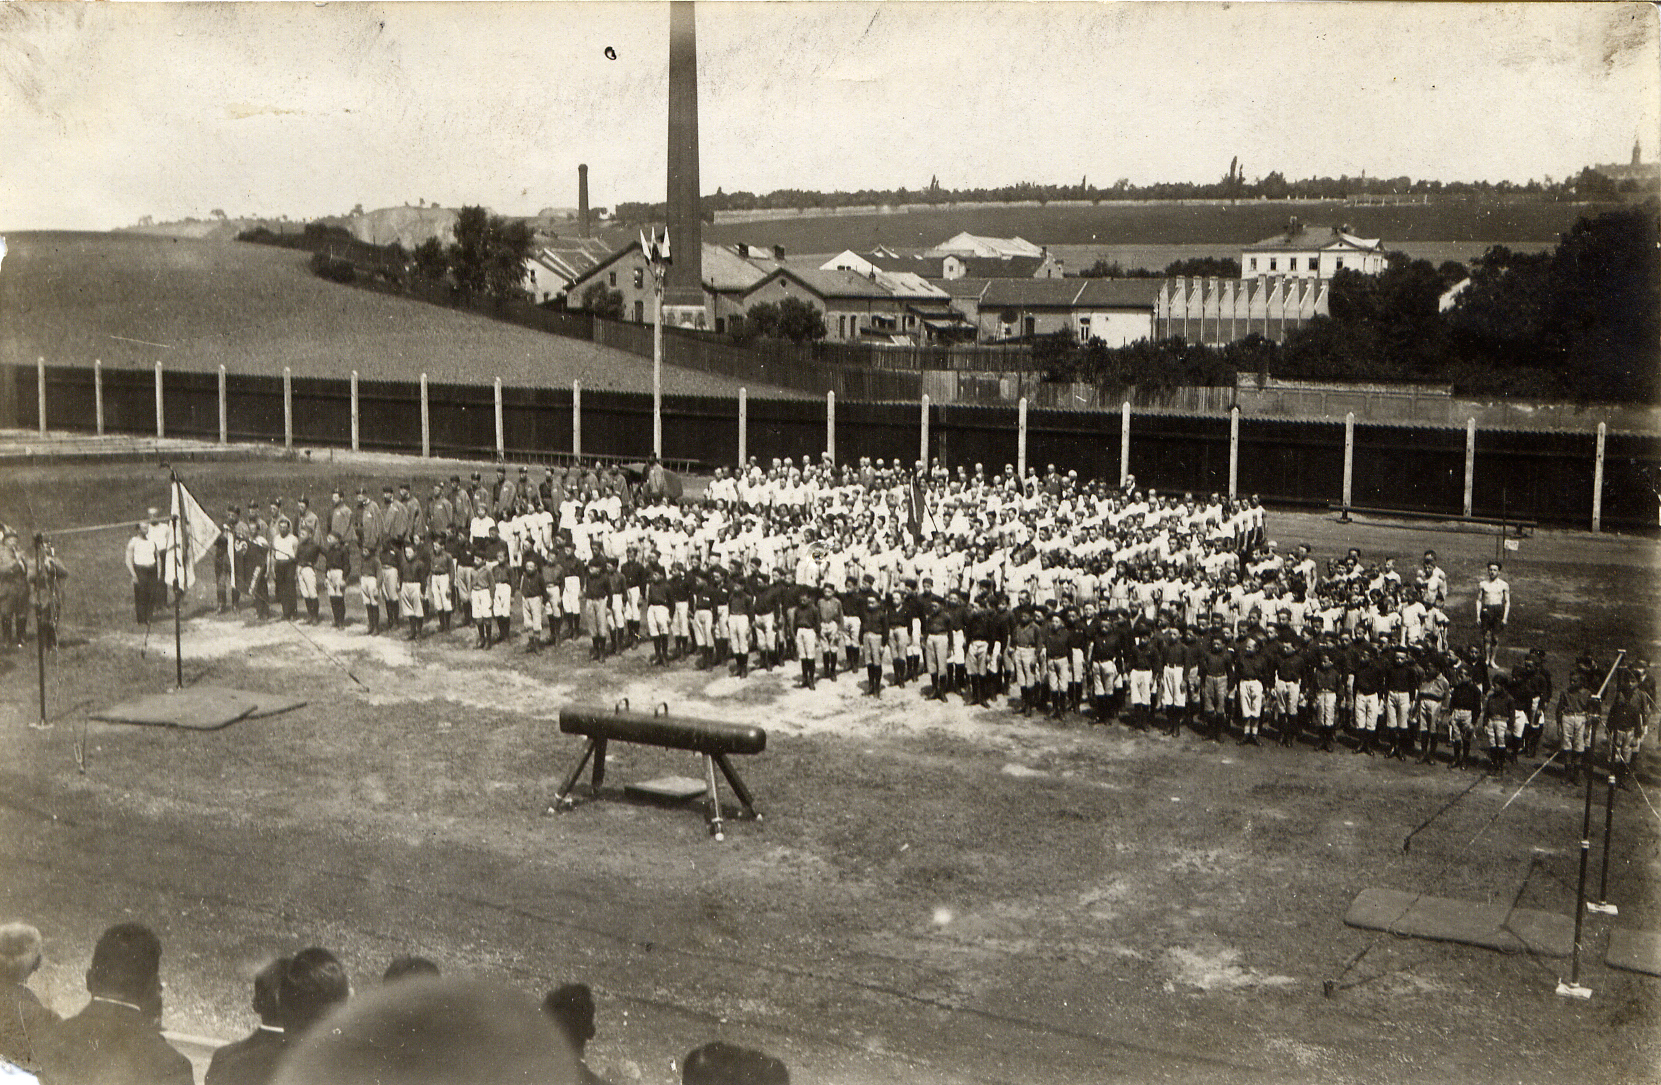
\includegraphics[width=0.9\textwidth]{img/26_otevreni_cviciste.jpg}
  \caption*{Slavnostní otevření letního cvičiště (1924), foto: archiv T.~J.
  Sokol Libeň}
\end{figure*}

Firmě Grab a synové jednota platila deset roků vysoké nájemné. Chtěli
jsme pozemek odkoupit, firma však požadovala 1\,000\,000\,Kč. Jakou cenu by
měl dnes? Teprve v~roce 1933, když Pražská obec převzala pozemek do
svého vlastnictví, byly oba pozemky odkoupeny a cvičiště bylo opravdu
naše. Pak došlo k~další definitivní úpravě cvičiště a vydání 250\,000\,Kč
bylo kryto povinnou daní 12\,Kč pro člena ročně a 6\,Kč pro dorost a
žactvo po dobu 5 roků.

Od té doby se začalo v~libeňském Sokole dařit lehké atletice a hrám,
zejména házené, později i odbíjené. Od roku 1924 se konaly na našem
"letním cvičišti" v~září celopražské závody lehkoatletické a soutěže
v~házené. Na prvních startovalo 156 mužů a 94 dorostenců, dále ženy a
dorostenky. Házené se zúčastnilo 14 družstev dorostenců. Slavných
podzimních libeňských atletických závodů se zúčastňovali i význační
atleti jako Evžen Rošický, Kněnický, Dostál, Hron, Chmelík aj., z~našich
to byl MUDr. Svatoš, který reprezentoval naši republiku i za hranicemi.

\subsection{Meziválečné slety na Strahově}

\textbf{VIII. všesokolský slet (1926)} se konal poprvé v~Praze na
Strahově. Ten už mnozí z~nás dobře pamatují (\pozned{již tomu tak dávno
není, pozn. ed.}). Cvičili jsme na něm jako dorost nebo žactvo a ti
nejstarší jako členové nebo členky. Na sletové dny žactva 13.~června
vysílá Libeň 128 žáků a 136 žákyň. Do závodů na chůdách se dostal mezi 5
nejlepších náš žák Karel Jeřábek, jakožto vítěz za župu Barákovu.

Sletové dny dorostu se konaly 27. a 29.~června 1926. Z~Libně cvičilo 72
dorostenců prostná, 7 dorostenců v~bojovém závodě družstev a 4
jednotlivci v~pětiboji. Donesli 1 plaketu a 6 diplomů. V~závodu
zvláštním se vyznamenal dorostenec Moravec. Byl prvním ve skoku dalekém
z~místa (310 cm) a druhý ve skoku vysokém z~místa (114 cm). V~běhu
rozestavném (štafetě) bylo naše družstvo třetí. Dorostenky závodily
v~odbíjené a ve štafetě. Prostná jich cvičilo 69.

\medskip
Ve hlavních sletových dnech:
\medskip

\noindent
3.~7. cvičilo naše žactvo a dorost ve velkém počtu

\noindent
4.~7. cvičilo 126 mužů prostná a 46 starších mužů s~tyčemi a dále 111
žen prostná

\noindent
5.~7. nastupuje 40 našich mužů v~čele proudů a 73 žen na prostná

\noindent
6.~7. cvičí prostná 92 mužů a 81 žen. V~župním vystoupení s~kroužky
cvičí 80 žen
\medskip

\begin{figure*}[h!]
  \centering 
  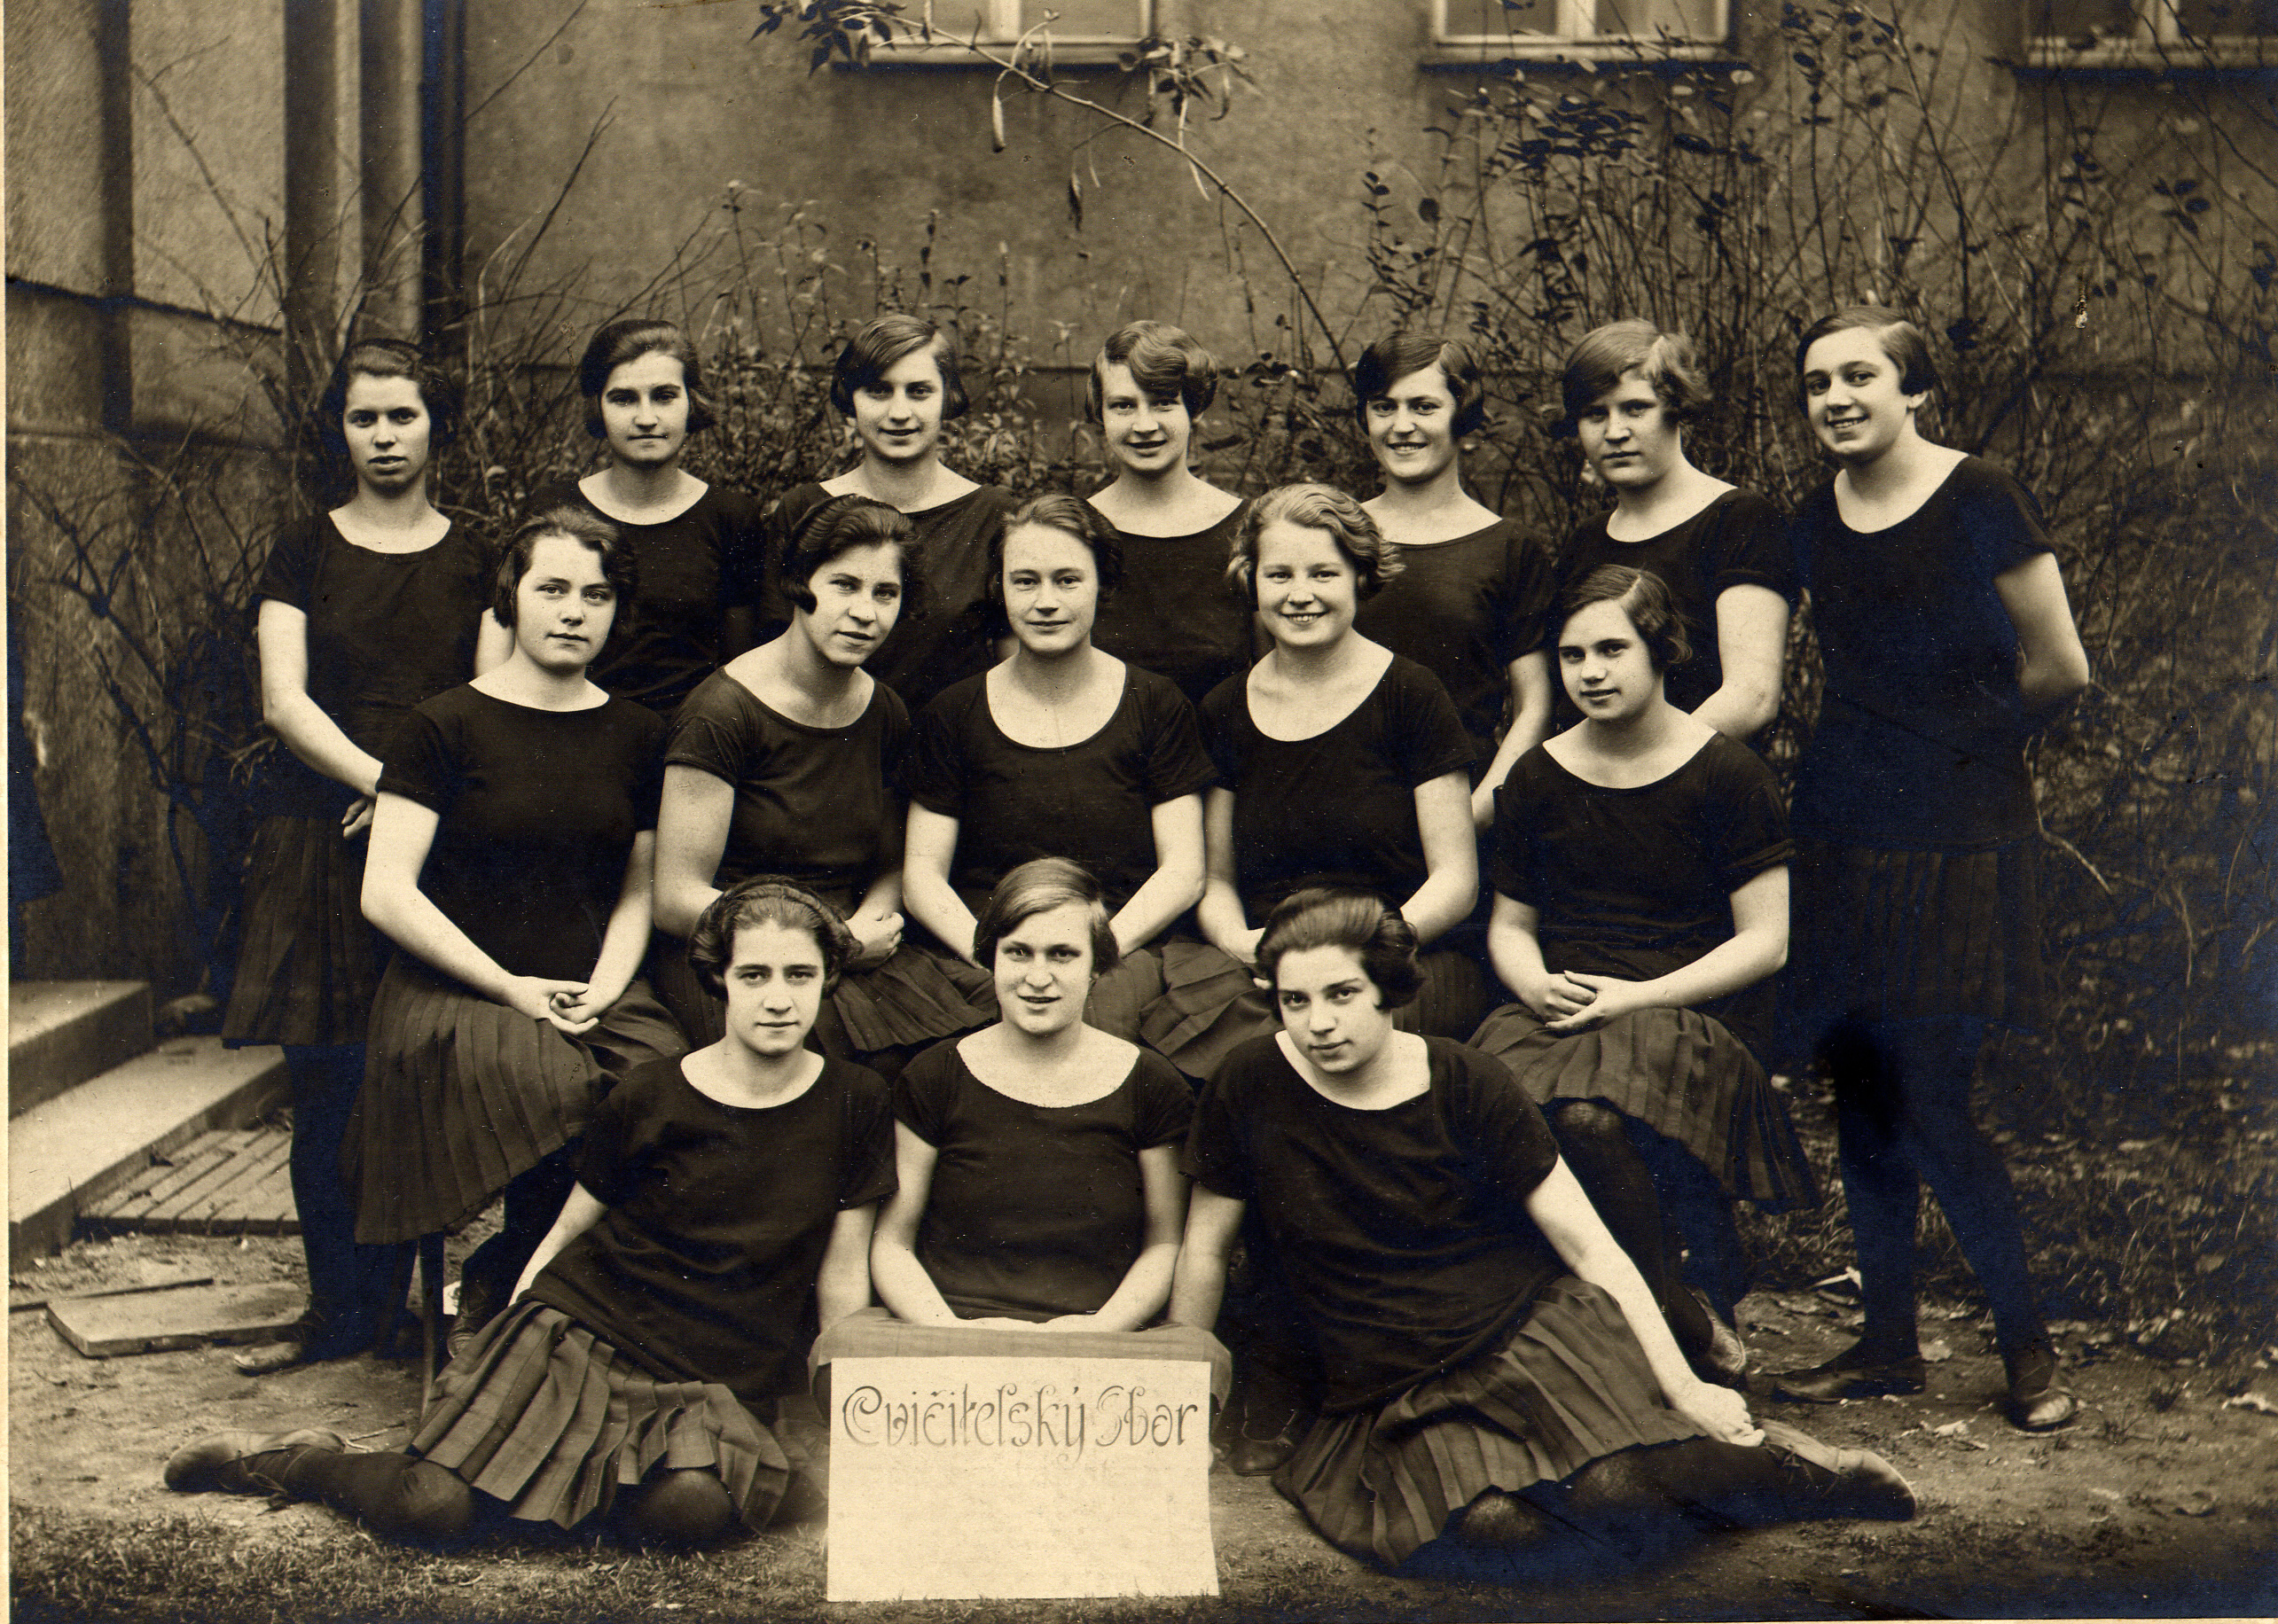
\includegraphics[width=0.9\textwidth]{img/27_dorostenky.jpg}
  \caption*{Cvičitelský sbor dorostenek (1926), foto: archiv T.~J. Sokol
  Libeň}
\end{figure*}

Ve vystoupení Pražského pětižupí dne 20.~června cvičí naši muži i ženy
ve velkém počtu. Ve sletové scéně účinkovalo 93 mužů a 20 dorostenců, 20
žen a 10 dorostenek. O~ubytování 2\,614 mužů a 1\,227 žen v~libeňských
školách se staralo 26 našich členů. Na celonoční hlídání sokolského
stadionu na Strahově jsme 12.~června vypravili 54 mužů. Nebudeme všechny
slety takhle podrobně popisovat -- nelekejte se. Ale alespoň na jednom
musíme ukázat, kolik práce dají jen ty sletové dny a kolik práce a
námahy to stojí před sletem.

Po sletě organizoval Sokol v~Libni své každoroční podzimní
lehkoatletické závody a soutěže v~házené, zúčastňoval se dalších
sokolských podniků v~Praze i mimo Prahu, obsazoval rozestavný běh
Praha--Mělník a hvězdicový závod k~oslavám 28.~října. Připravoval na přání
rodičů taneční hodiny pro náš dorost, pomáhal s~besídkami dorostu, pro
žactvo zařídil loutkové divadélko a vyvíjel a vymýšlel stále nové a nové
činnosti.

Také v~Sokole jsou léta dobrá --⁠⁠⁠⁠⁠⁠ radostná i léta zlá. V~libeňském Sokole
převládala léta radostná. Již k~25. výročí založení Sokola
(1909--1910) vystavěli si libeňští hezkou a moderní
sokolovnu. K~40. výročí (1924) vybudovali pěkné letní cvičiště, na
kterém každoročními podzimními závody v~lehké atletice a ve hrách bylo
rozšiřováno dobré jméno Sokola Libeň. O~to dobré jméno se postarala i
libeňská loutková scéna. Zásluhou Dr. Jana Malíka a řady jeho % libeňská loutková scéna
vynikajících spolupracovníků se dostala mezi nejpřednější scény nejen
v~Praze, ale i v~celé republice. Primát jí potvrdil sám prof. Josef Skupa
zápisem v~Pamětní knize loutkářů. V~roce 1931 a také v~dalších letech se
zde konaly loutkářské školy ČOS za účasti více než 200 sokolských
loutkářů. Tehdy bylo v~ČOS na 2\,000 loutkových divadel. Moderně vybavená
scéna i stupňovité hlediště bývalo v~nynějším Srncově sále, pojmenovaném
po Ing. Antonínu Srncovi, který byl duší elektrického osvětlení a
vynálezcem všech světelných efektů ve scéně. Hrávalo se v~neděli
odpoledne pro děti (ve 14 a 16 hodin) a někdy večer pro dospělé. Z~mnoha
her jsou ještě v~naší paměti: Jiráskova Lucerna, Kvapilova Princezna
Pampeliška, Král Oidipus a zejména Pomněnky. Z~dětských her všechny hry
s~Kašpárkem a nejrozšířenější Malíkova hra Míček Flíček. Konstrukce
provedená podle návrhu Dr. Malíka se stala vzorem mnoha dalším loutkovým
scénám.

Zprávy tělocvičné jednoty Sokol v~Praze Libni začaly vycházet v~roce
1927 nákladem 1\,200 kusů, 10 čísel za rok. Členové je dostávali zdarma.
Prvním redaktorem byl Dr. František Bulánek. Všechny sletové roky byly
pro nás těmi roky radostnými. Strahovské sletiště, postupně mezi slety
dodělávané, je tím největším stadiónem na světě. Poprvé se na něm konal
VIIl. slet v~roce 1926. Tehdy už ČOS sídlila v~nově vybudovaném Tyršově
domě v~Praze na Malé Straně (arch. Krásný, 1925). Své sídlo zde měla i
naše Barákova župa i Tyršovo muzeum.

\begin{figure*}[h!]
  \centering 
  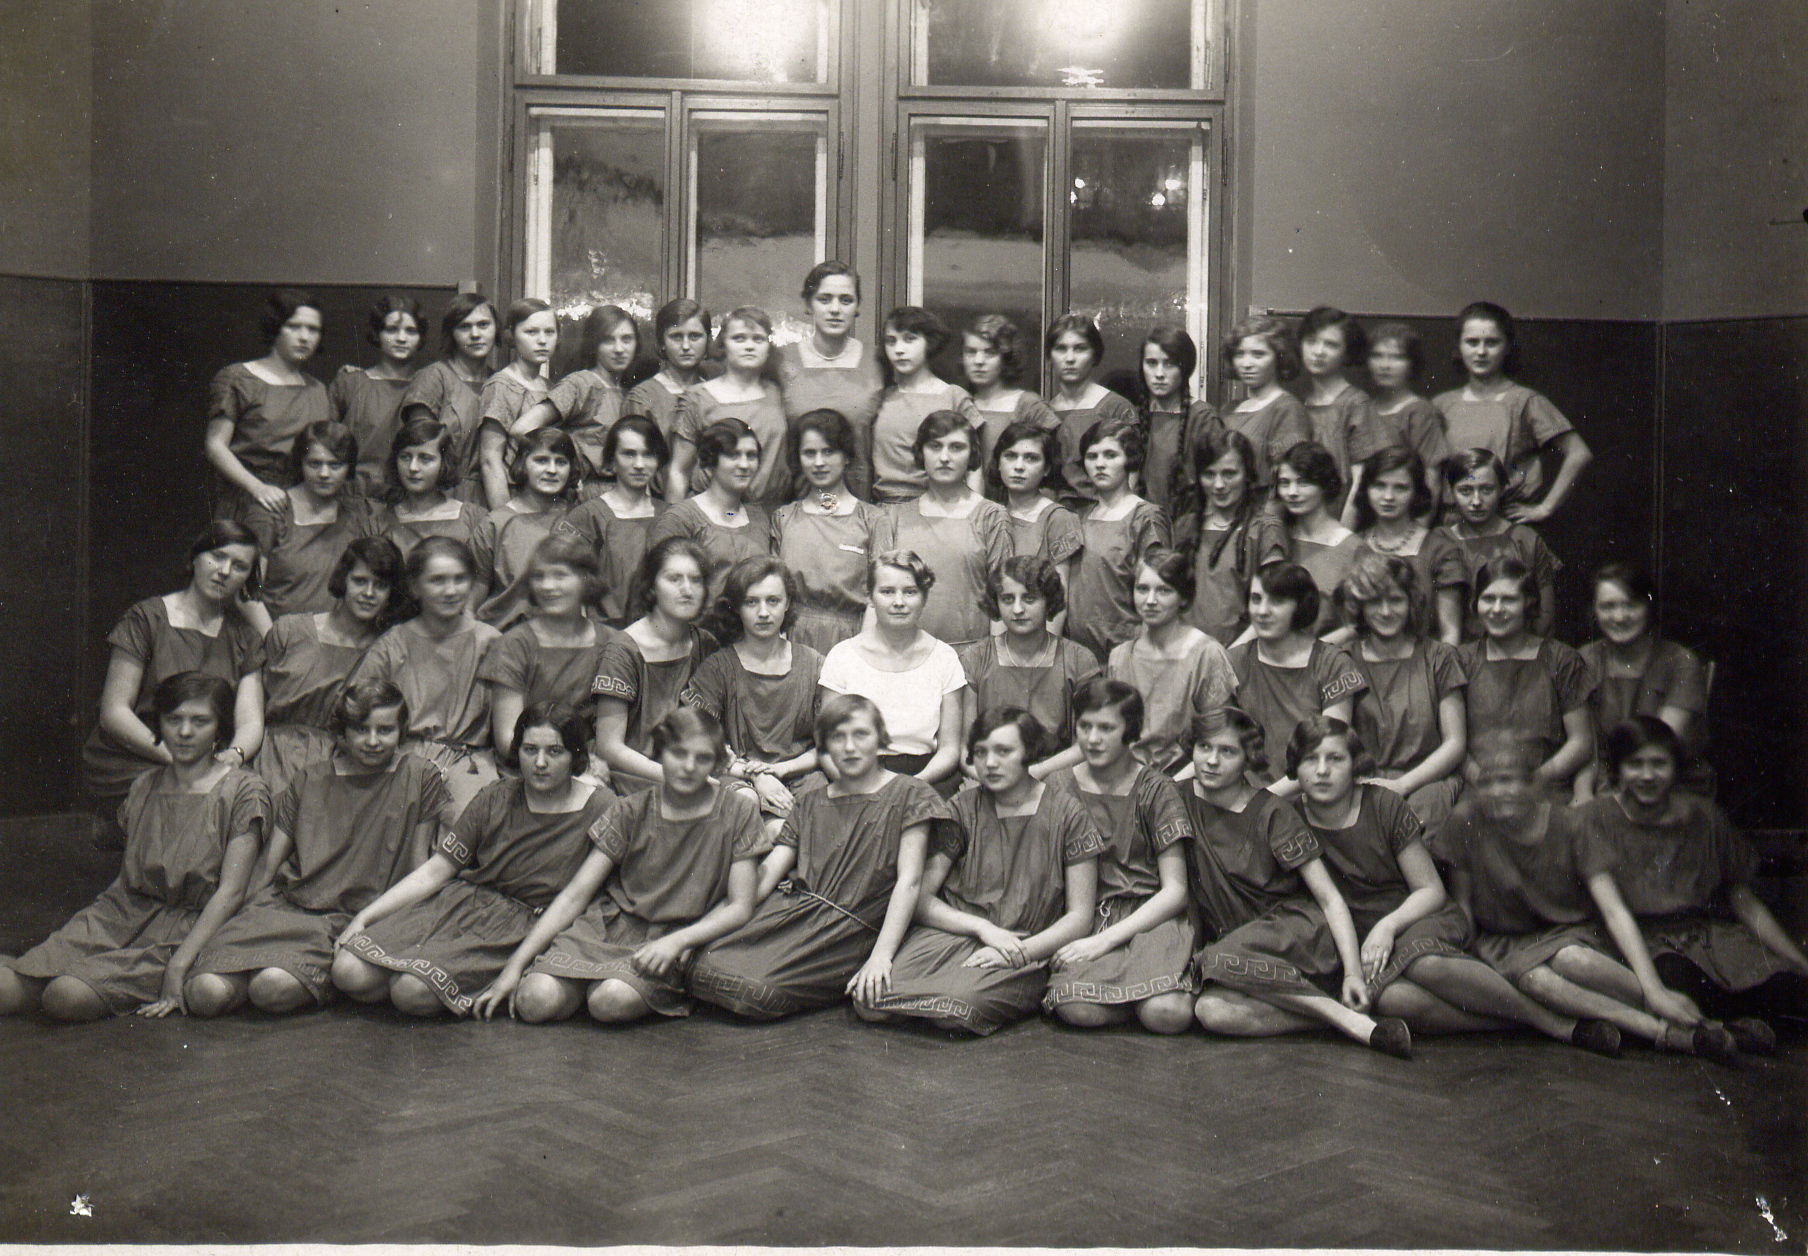
\includegraphics[width=0.9\textwidth]{img/28_dorostenky.jpg}
  \caption*{Dorostenky (1928), foto: archiv T.~J. Sokol Libeň}
\end{figure*}

\textbf{IX. všesokolský slet 1932 -- Strahov}. Krásou, počtem diváků i počtem cvičících předčil všechny slety minulé.
Konal se v~roce 100. výročí narození Dr. Miroslava Tyrše a v~roce 70.
výročí založení Sokola. Sletu předcházel Sletový rozestavný běh v~září
1931. Na 9 trasách z~měst v~pohraničí i ze Slovenska běželo na tratích
o~délce 3\,500 km skoro 40\,000 běžců. Libní probíhaly dvě trasy a na ně
jsme stavěli 54 běžců dospělých i z~dorostu. V~květnu jsme již cvičili
sletová prostná na Okrskovém cvičení v~Měšicích. Naše účast tu byla
veliká -- 718 (žactvo, dorost a členstvo). O~týden později byl v~Libni
Župní slet žactva (307 z~Libně) a za čtrnáct dní (22.~května) jsme
uspořádali na našem letním cvičišti Veřejné cvičení -- 878 cvičících.

Na Strahově nás z~Libně cvičilo 792 a dalších 200 vystupovalo v~nádherné
sletové scéně "Tyršův sen". Byla uvedena celkem osmkrát a pokaždé v~ní
účinkovalo asi 5\,000 cvičících. Oproti roku 1926 se počet cvičících
z~Libně zvedl o~25 \% na 992 cvičenců. Kolik radosti a hezkých trvalých
vzpomínek si všichni odnesli, to se vyčíslit nedá.

\begin{figure*}[h!]
  \centering 
  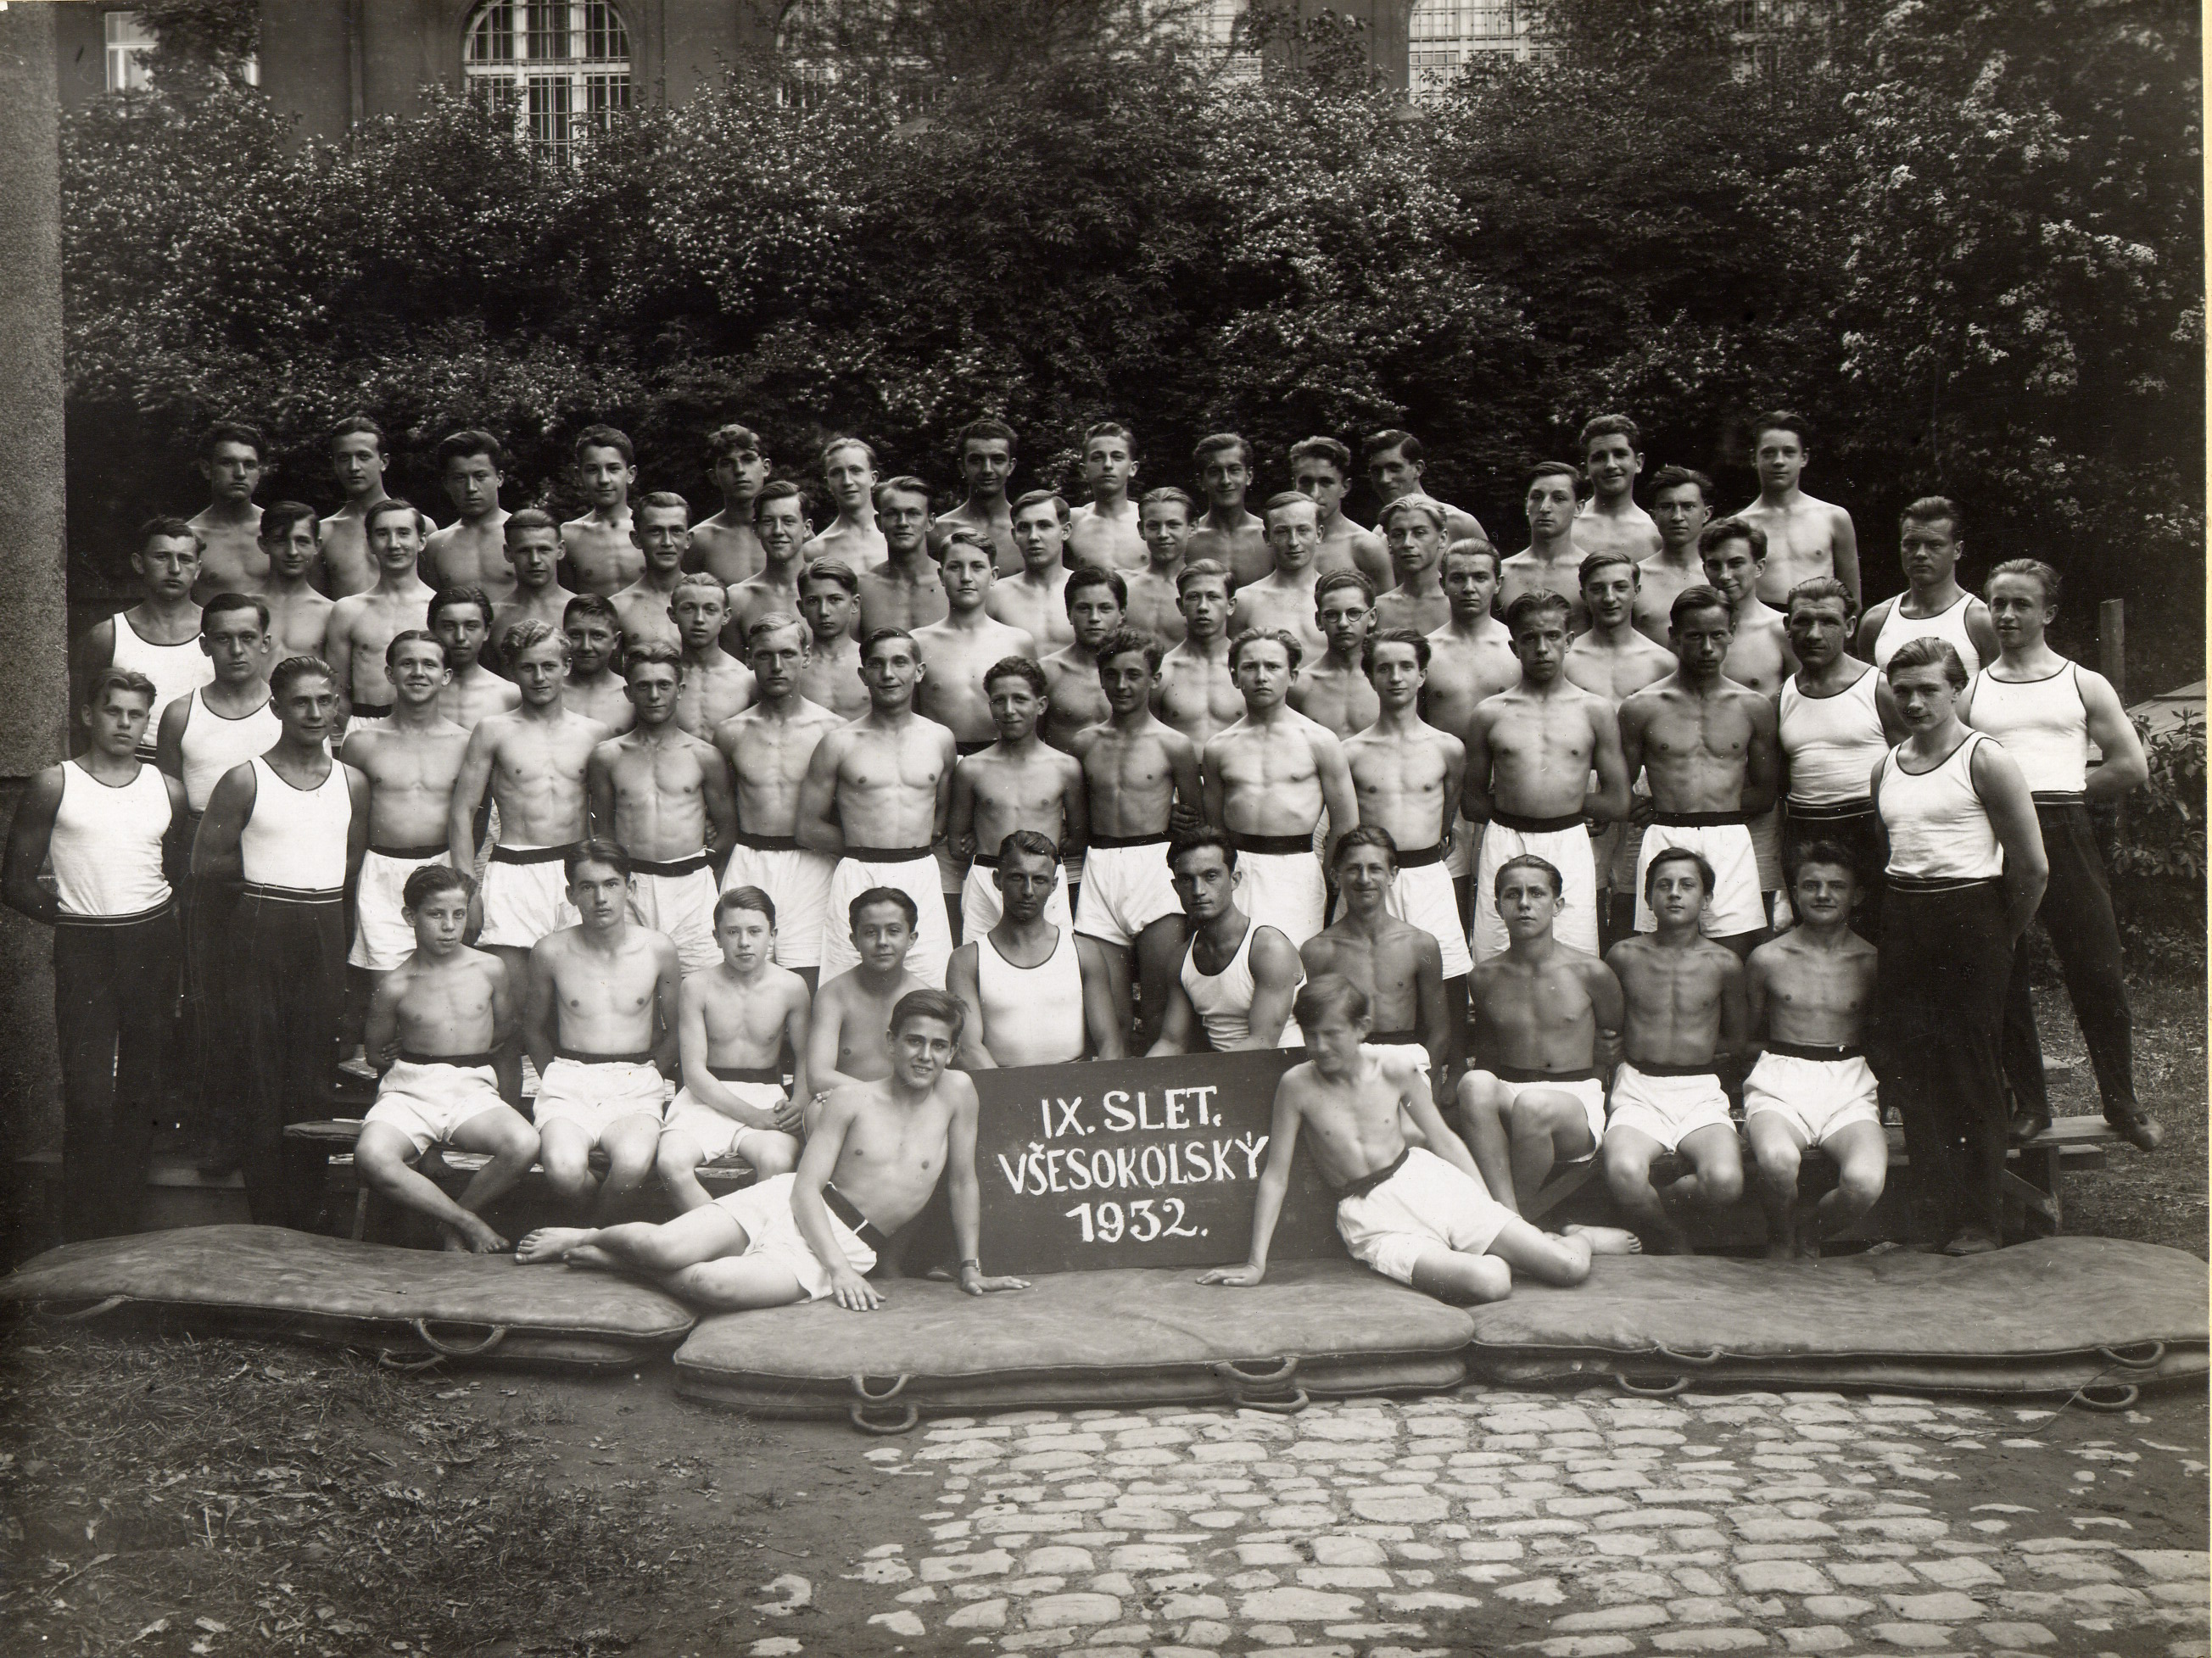
\includegraphics[width=0.9\textwidth]{img/29_muzi_slet.jpg}
  \caption*{Muži slet 1932, foto: archiv T.~J. Sokol Libeň}
\end{figure*}

Sletové závody jsme také dobře obeslali. Naše družstvo mužů získalo 2.
místo v~přetahu lanem. Mladý František Svatoš získal první místo v~běhu
na 100 m a dvě druhá místa -- běh na 200 m a skok daleký. Úspěšně
závodili i naši dorostenci a dorostenky, které dosáhly přes 85\,\%
dosažitelných bodů. Ale sletem činnost v~Sokole neskončila. Následovala,
jako vždy, řada akcí a soutěží v~atletice, ve hrách, besídky a akademie,
výlety, zábavy aj.

\begin{figure*}[h!]
  \centering 
  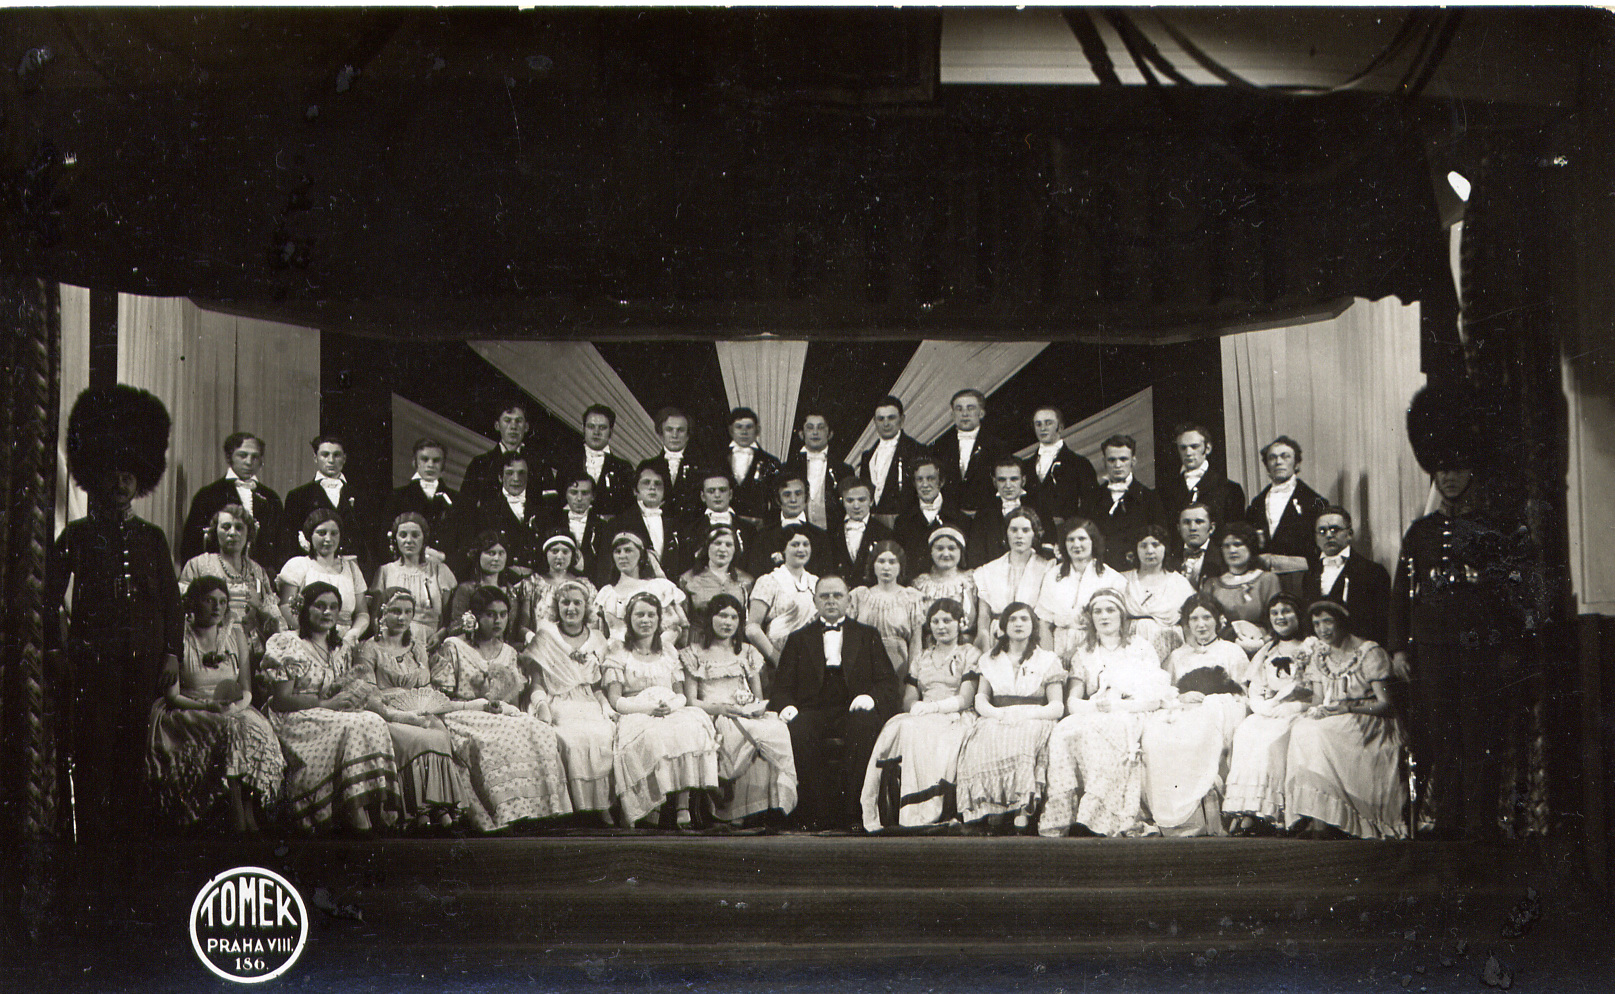
\includegraphics[width=0.9\textwidth]{img/30_sibrinky.jpg}
  \caption*{Šibřinky 1932, foto: archiv T.~J. Sokol Libeň}
\end{figure*}

\textbf{Rok 1934 -- 50. výročí založení Sokola v~Libni}. Oslavy tak významného jubilea byly zahájeny již 21.~října na libeňském
hřbitově položením vavřínového věnce na hrob prvního starosty Josefa
Voctáře. Zazněly lesní rohy, zapěl spolek Věnceslav a starosta jednoty
br. Švejda připomněl zásluhy br. Voctáře i všech zakládajících členů
naší jednoty.

V~sobotu 27.~října večer se konala v~sokolovně Slavnostní akademie.
První část byla věnována recitacím, zpěvu a hudbě. Účinkovali v~ní
vynikající umělci, např. člen ND Karel Kollár, pěvecký sbor Věnceslav,
Orchestrální sdružení Sokola v~Praze 7. Druhá část akademie byla
tělocvičná, na ní vystupoval náš dorost a členstvo. Skladby byly dílem
domácích autorů: náčelnice Boženy Srncové a Marie Danihelkové a
náčelníka Vojty Vacína a Oldřicha Čupra. Hudbu ke cvičení složil a
klavírní doprovod obstarával Dr. Jiří Kvaček. (\textit{Povšimněte si,
kolik libeňských ulic je pojmenováno po libeňských sokolech, pozn. ed.})

V~neděli 28.~října -- den 20. výročí Československé republiky -- se
konala ráno tryzna za padlé v~l. světové válce a v~10 hodin byla
zahájena slavnostní jubilejní valná hromada. Byla otevřena rozsáhlá
výstava a vydán Památník 1884--1934. Žactvo začalo své oslavy
na letním cvičišti a potom vyslechlo v~sokolovně pohádku vzdělavatele
Dr. Malíka o~rytířích a zvláštním hradu -- první sokolovně v~Praze.
Přátelským večerem byly zakončeny oslavy půlstoleté činnosti sokolské
jednoty v~Libni. Jen výstava ještě pokračovala a během týdne ji shlédlo
na 2\,000 osob.

22.~září 1935 byl odhalen před libeňským zámkem, kdysi letním sídlem
pražských primátorů, pomník doktoru Janu Podlipnému, prvnímu starostovi
České obce sokolské a Svazu slovanského sokolstva, primátoru královského
města Prahy. Dopolední průvod šel z~Balabenky přes Palmovku k~zámku.
Pochodovalo v~něm 412 krojovaných sokolů za 7 prapory a se čtyřmi
hudebními sbory. Slavnostním řečníkem byl starosta župy Barákovy br. Fr.
Mašek. Památník zbudovaný Spolkem pro zbudování pomníku je dílem sochaře
Jaroslava Brůhy a našeho člena arch. Jana Bloudka. V~předvečer odhalení
památníku se konal v~sokolovně slavnostní večer s~bohatým kulturním
programem. Promluvil na něm starosta ČOS Dr. Bukovský.

Radostné roky, které jsme prožívali ve 30. letech, měly přece jen nějaké
kazy. Byla to světová hospodářská krize spojená s~nezaměstnaností a pak
doba nástupu Hitlera k~moci v~roce 1933. Svět se právem obával německé
rozpínavosti a usilovně zbrojil. V~sokolských jednotách byla zaváděna
branná cvičení, konaly se branné srazy, pochodová cvičení, výcvik ve
střelbě, ošetřovatelské kurzy apod. Stát budoval mohutná opevnění, celý
národ pochopil nebezpečí doby a opravdu se semknul k~obraně vlasti.
Zejména po násilném obsazení Rakouska dělali Němci v~pohraničí velké
výtržnosti. Dostávali jsme o~tom nedobré zprávy od naší svěřenky --
Sokol Trmice u~Ústí nad Labem. V~květnu roku 1938 byla vyhlášena
částečná mobilizace a v~takovém ovzduší začínal náš dosud nejkrásnější a
největší všesokolský slet. Tak velký, že muži cvičili ve skladbě
"Přísaha republice" i mezi značkami v~počtu 28\,600. Ženy nezůstávaly
pozadu, v~úchvatném reji vystoupilo 28\,640 žen. Všech cvičících na sletě
bylo 1\,034\,800 (v~roce 1932 -- 18\,800) a diváků bylo 2\,300\,000.

\textbf{X. všesokolský slet 1938 -- Strahov}. Také tento slet byl zahájen již v~říjnu 1937 rozestavným během na deseti
trasách o~délce 4\,185 km. Z~Tyršova domu neslo poselství 42\,000 běžců do
pohraničních měst i na Podkarpatskou Rus. Libeňský Sokol stavěl 72 běžců
a 72 světlonošů, neboť se běželo i v~noci.

{\sloppy Nácvik sletových skladeb začínal na podzim a pokračoval celou zimu.
V~dubnu se již dělaly prověrky znalostí prostných a v~květnu bývaly
okrskové a župní slety. V~Libni na hřišti Meteoru byl 8.~5. župní slet
žactva za účasti 5\,000 cvičenců. 15.~5. předsletový večer na letním
cvičišti v~Libni s~ukázkami cvičení sletových. Župní slet byl 5.~6.
v~Lysé nad Labem. Náš dorost se zúčastnil sletových plaveckých závodů a
župních závodů v~atletice. \par}

\medskip
Hlavní činnost se soustředila na vlastní slet:
\medskip

16.~6. den brannosti (naše účast 160)

19.~6. průvod žactva

20.~6. slet žactva (279 žáků a podobný počet žákyň).

\medskip
Také náš dorost měl velký podíl na úspěchu sletu. Prostná mužů cvičilo
106 mužů, ženy vystupovaly třikrát, průměrně 150 žen. Naše účast
v~průvodech žactva, dorostu i členstva byla vždy veliká, nechceme však
unavovat čísly. Za zmínku stojí ještě podíl libeňských loutkářů na
sletu. Získali první místa v~soutěži ČOS hrou "Sletu zdar" (95 bodů ze
100 možných). Dr. Jan Malík byl autorem sletové scény X. sletu nazvanou
"Budovat a bránit", ve které účinkovalo 5\,000 osob.

\section{Období let 1938--1948}

Vrátíme se zpět do roku 1938, do období posletového. Válečné nebezpečí
se tak vystupňovalo, že 23.~září v~pozdních večerních hodinách vyhlásil
rozhlasem prezident Beneš mobilizaci. Ráno byli vojáci u~svých
vojenských útvarů. Taková byla kázeň a nadšení všech sokolů i celého
národa k~obraně vlasti. Sletová skladba "Přísaha republice" z~úst 28
000 mužů nevyzněla naprázdno. Několik dní po vyhlášení mobilizace se
konala konference v~Mnichově, kde Anglie a Francie jednala s~Hitlerem "o
nás, ale bez nás". Bylo nám doporučeno, ba skoro nařízeno, odstoupit
Hitlerovi naše pohraničí, aby se prý zabránilo válce. Nadšení vojáků se
změnilo v~bezmocnost a smutný návrat domů.

Zabrané pohraničí muselo rychle opustit mnoho českých a sokolských rodin
a jen s~uzlíčkem nejnutnějšího spěchalo do vnitrozemí ke svým známým.
Vzrůstal počet nezaměstnaných, pro které se hledala práce a pro které
byly vytvořeny Pracovní tábory. Jeden takový tábor zabral 26.~října 1938
libeňskou sokolovnu, takže veškerá činnost v~jednotě byla zastavena.
Výbor svolal na 15.~prosince mimořádnou valnou hromadu do školy Na
Korábě. Měly být řešeny otázky zabrání sokolovny a současná situace
v~jednotě a sokolstvu. V~té době totiž vznikal, bez účasti výboru ČOS,
první pokus o~sjednocení tělovýchovy. Byl ustaven Svaz občanské
pohotovosti (SOP) a bylo třeba tyto samozvance odmítnout. Pracovní tábor
uvolnil naši sokolovnu až v~dubnu 1939.

\subsection{II. světová válka 1939--1945}

Mnichov válce nezabránil, ani námi odstoupené pohraničí. 15.~března 1939
stanul Hitler v~Praze a prohlásil Čechy a Moravu za protektorát německé
říše. Den předtím se odtrhlo Slovensko, prohlásilo se samostatným státem
a Tiso požádal Hitlera o~ochranu. Druhá nejhroznější světová válka byla
odstartována, o~Velikonocích 1941 byla zastavena činnost sokolských
jednot. K~hromadným zatýkáním sokolů došlo v~noci z~8. na 9.~října 1941.
Gestapo zatýkalo současně po celém území protektorátu především
činovníky ČOS a žup. Na 1500 sokolů bylo té noci zatčeno.

Mezi zatčenými byl i náčelník župy Barákovy Vojta Vacín a starosta župy
Jaroslav Řepa. Oba zemřeli v~koncentračním táboře v~Osvětimi. Bratr Řepa
4.~dubna 1942, br. Vacín o~několik dní později. Bratru Řepovi bylo 47,
Vacínovi 55 let.

Po celou dobu okupace se zatýkalo a posílalo se do koncentráků a na
smrt. Nejhorší to bylo po atentátu na říšského protektora Heydricha
v~roce 1942, kdy i jen za projevený souhlas s~atentátem byla smrt. Jména
libeňských obětí jsou na mramorové desce v~hale sokolovny. Nejmladšímu
z~obětí bylo 20 let a zemřel nejdříve, nejstaršímu bylo 70 let a zemřel
jeden den před naším osvobozením. Na ně nesmíme zapomínat.

\subsection{Sokolské oběti nacistické okupace v~Libni}

\textbf{Vojta Vacín} (nar. 16.~7. 1887), náčelník župy Barákovy,
dlouholetý náčelník libeňské jednoty, od svého mládí nadšený cvičenec.
Umučen v~koncentračním táboře v~Osvětimi 17.~5. 1942 (55 roků).

\textbf{Bohuslav "Sláva" Strnad} (nar. 1.~3. 1905), náčelník Sokola
v~Libni. Zatčen 2.~7. 1942 pro účast na atentátu na Heydricha, po
nejtěžším nacistickém mučení popraven 24.~10. 1942 se svou manželkou
Marií. Bratru Strnadovi bylo 37 roků.

\textbf{Josef Decastello} (nar. 24.~6. 1910), plukovník čs. armády,
letec. Vzorný cvičenec. Byl vyznamenán Čsl. válečným křížem a franc.
Croix de Guerre. Sestřelen nad Francií nešťastnou náhodou
francouzskou protivzdušnou obranou 3.~6. 1940 (30 let).

\textbf{Otomar Kefurt} (nar. 10.~11. 1886), řídící učitel, tvrdý a
nezlomný vlastenec. Za ukrývání ilegálního pracovníka byl 3.~12. 1943 na
Pankráci sťat se svou ženou Annou Kefurtovou. Bratru Kefurtovi bylo 57
roků.

\textbf{Čeněk Kníže} (nar. 11.~2. 1895), padl 7.~5. 1945 na mostě
Barikádníků. Bylo mu 50 let.

\textbf{Tomáš Míchal} (nar. 23.~12. 1906), obětavý člen naší loutkové
scény. Zatčen 15.~8. 1941, uvězněn v~Terezíně, zemřel v~koncentračním
táboře v~Mauthausenu v~roce 1942 ve věku 36 let.

\textbf{Ing. Antonín Srnec} (nar. 22.~5. 1902), jeden z~nejlepších
cvičenců a cvičitelů jednoty, technický spolupracovník naší loutkové
scény, důstojník čs. armády. Účastnil se jako jeden z~prvních bojů na
barikádách, byl velitelem v~oblasti Slovanka, kde padl 7.~5. 1945 ve
věku 43 roků.

\textbf{Miloslav Vitouš} (nar. 10.~1. 1902), dlouholetý člen naší
jednoty. Zatčen 4.~6. 1942, odvezen na Pankrác a 6.~6. 1942 popraven na
střelnici v~Kobylisích ve věku 40 let.

\textbf{Václav Vopička} (nar. 31.~10. 1875), člen naší a prachovické
jednoty. Se svou ženou zatčen 25.~1. 1945 v~Prachovicích, obviněn
z~přechovávání parašutistů. Zemřel v~předvečer našeho osvobození, 8.~5.
1945 v~Terezíně. Bylo mu 70 let.

\textbf{Irena Brillová} byla odvlečena do Terezína, kde v~roce 1942
zemřela s~celou svojí židovskou rodinou, protože Židé, podle nacistů,
neměli právo žít.

Po zastavení činnosti Sokola v~roce 1941 byla zabrána naše sokolovna na
skladiště vojenského leteckého materiálu. Ve všech místnostech sokolovny
bylo několik vagonů materiálu. Němci naši budovu nešetřili. Po vyklizení
všeho v~červenci 1945 se ukázala hrozná spoušť. Voda netekla, odpady
byly ucpané, podlahy, zámky, vypínače a všechno zničené. Uvedení do
přijatelného stavu stálo mnoho práce a peněz. Cvičit se začalo nejdříve
na letním cvičišti, později v~gymnáziu a teprve v~prosinci v~sokolovně.
S~velkým nadšením se začínalo. Byl ustaven lyžařský oddíl, vedený Jiřím
Štěpničkou a Mirkem Vaňkem a 20 lyžařů trávilo první Vánoce v~chatě jimi
získané v~Dolní Malé Úpě v~Krkonoších. K~31.~12. 1945 uvádí matrikář
Ludvík Holý stav členstva včetně dorostu a žactva celkem 2\,889 duší,
z~toho 1\,303 dospělých, 430 dorostu a 1\,156 žactva. Starostou byl Dr.
Štross, náčelníkem Jar. Jirák, náčelnicí B. Votýpková.

V~roce 1945 byl zvolen výbor naší jednoty s~těmito funkcemi:

\medskip
Jiří Štross -- starosta

Sláva Veger -- místostarosta

Bohumil Andrle -- jednatel

Josef Mrklas -- pokladník

Ludvík Holý -- matrikář

Helena Andrlová -- vzdělavatel

Jan Koubek -- správce sokolovny

Jaroslav Kubišta -- správce osvětlení

Miroslav Procházka -- archivář

Jindra Vajkrt -- vedoucí pořadatelského sboru

Jaroslav Jirák -- náčelník

Boženka Votýpková -- náčelnice
\medskip

Výbor sokolské jednoty na své první schůzi v~roce 1945 stanovil program
obnovy sokolovny. Řízením prací na její obnově byli pověřeni starosta
br. Štross a správce osvětlení br. Jar. Kubišta. Do úklidu sokolovny se
tehdy pustili všichni členové jednoty, včetně žactva a dorostu. V~této
době bylo nutné opravit střechu, udělat novou elektroinstalaci a nové
osvětlení, vymalovat všechny místnosti a opravit nářadí. Práce
elektrotechnické byly svěřeny instalačnímu odboru Elektrických Podniků
hl. m. Prahy. Byla vyměněna starodávná osvětlovací tělesa a vypínače na
klíček za moderní. Nová elektroinstalace byla provedena v~mědi. Napětí
120 V~byla vyměněno na 220 V. Nové osvětlení ve velkém sále bylo
ovládáno dálkově ze dvou míst u~jeviště a ve sborovně. Tyto moderní
rozvaděče a reflektory darovala firma Vohralík (člen Sokola) a výrobce
divadelního osvětlovacího zařízení. Od firmy "Philips" byla instalována
telefonní ústředna pro 10 telefonních stanic (tzn. 1+10). Telefony byly
umístěny ve sborovně, v~úřadovně, ve Filipově síni, u~sokolníka atd.
Celá sokolovna byla velmi vkusně vymalována podle návrhu bratra Ing.
arch. J. Jakuba. Práce malířské provedla firma Franěk (člen jednoty).
Veškeré nářadí pro cvičení bylo znovu opraveno a instalováno, takže se
mohlo ihned začít cvičit. Později byla opravena střecha sokolovny
z~mědi. K~znovuotevření sokolovny byly vydány odznaky podle návrhu br. M.
Haufa. Byly velmi vkusné a byly také ihned rozprodány.

Nadšení všech členů jednoty při obnovování naší sokolovny bylo
příkladné. Sokolovna v~této době byla v~nádherném stavu: nová malba,
nové osvětlení, moderní zařízení na ovládání světel ve velkém sále (při
pořádání tělocvičných akademií, besed, šibřinek atd.). Musím se zmínit
o~tom, že bývalí uživatelé od roku 1949 toto zařízení zrušili a v~roce
1989 (resp. 1991) nám předali sokolovnu opět v~žalostném stavu (zvláště
pro cvičící), bez telefonní ústředny a rozvaděčů s~moderním ovládáním
světel.

V~roce 1946 již nastává normální a hezký život v~tělocvičně i na letním
cvičišti. Kromě obvyklých besídek žactva a dorostu, výletů a zájezdů,
domácích i župních závodů na nářadí a v~atletice, turnajů v~házené a
odbíjené, školení cvičitelů v~jednotě, v~župě i v~ČOS tu byly i šibřinky
a jejich dozvuky, společenské podniky a všude i spolupráce Věrné gardy
(následovnice Staré gardy). Loutkáři přebudovali svoji scénu a od října
do konce roku sehráli dětem 25 představení. V~naší chatě v~Krkonoších
(dnešní Sokolí boudy) byla o~prázdninách první žákovská osada.
Dorostenci prožili 14 dní ve stanovém táboře na Sejckém ostrově na
střední Vltavě a po nich na stejném místě dorostenky.

Rok 1947 byl už rokem předsletovým. Cvičenců ve všech složkách přibývá,
cvičí se ve dvou až třech oddílech a ještě prostory nestačí. V~přehledné
tabulce uvádíme přesná čísla z~Výroční zprávy za rok 1947, str. 9.

K~31.~12. 1947 měl Sokol Libeň tento stav:


\setlength\LTleft{0.4cm}
\renewcommand*{\arraystretch}{1.1}
\begin{longtable}[]{%
  >{\raggedright\arraybackslash}p{2.7cm}%
  | >{\raggedleft\arraybackslash}p{1.5cm}%
  >{\raggedleft\arraybackslash}p{1.5cm}%
  >{\raggedleft\arraybackslash}p{1.5cm}%
  | >{\raggedleft\arraybackslash}p{1.5cm}}
{} &  členstvo &  dorost &  žactvo &  celkem \\
\hline
mužské složky &  1\,117 &  205 &  549 &  1\,871 \\
ženské složky &  1\,144 &  390 &  796 &  2\,330 \\
\hline
celkem &  2\,261 &  595 &  1\,345 &  4\,201 \\
\end{longtable}
\setlength\LTleft{0cm}

V~jedné cvičební hodině cvičilo průměrně:

mužů 155 ve 2 oddílech

žen 320 ve 3 oddílech

dorostenců 103 ve 2 oddílech

dorostenek 209 ve 2 oddílech

žáků 336 ve 3 oddílech

žákyň 509 ve 3 oddílech

3. oddíl žen cvičil dopoledne.
\medskip

{\sloppy Náčelníkem byl stále Jaroslav Jirák, místonáčelníkem František Kodl,
vedoucím dorostenců Ladislav Mrklas, vedoucím pořadatelského sboru
Jindra Vajkrt; matrikářem mužů Ludvík Holý. Dorost si vydával vlastní
časopis "Vzlet", měl svoji samosprávu, organizoval vlastní akademii, na
které byla dorostenkám předána nová vlajka s~heslem: "Národa být
jádrem". Na vlajku darovala stuhy Věrná garda. Náčelnicí byla Béda
Prokešová, jednou z~místonáčelnic Věra Decastellová. Mezi členkami
cvičitelského sboru jsou nám známé cvičitelky M.~Jiráková, M.~Kodlová,
Vl.~Kokošková, Vl.~Kubištová a V.~Haufová. Ve cvičitelském sboru mužů
byl i M.~Hauf, Lad.~Horáček a Jiří Žižka. \par}

Průběh cvičebního roku byl podobný roku předchozímu, ale byl
intenzivnější, zejména v~druhé polovině roku, kdy se již nacvičovalo na
XI. slet -- 1948. Členové museli projít ideovou školou a skládat slib.
28.~října 1947 složilo sokolský slib 79 bratrů a 74 sester. Také žactvo
-- 134 žáků a 46 žákyň -- slibovalo věrnost na svůj prapor. Na ideové
škole pro dorost i pro členstvo tehdy přednášeli člen předsednictva
vzdělavatelského sboru ČOS br. Jiří Janoš. Slib složilo 62 dorostenců a
62 dorostenek.

\begin{figure*}[h!]
  \centering 
  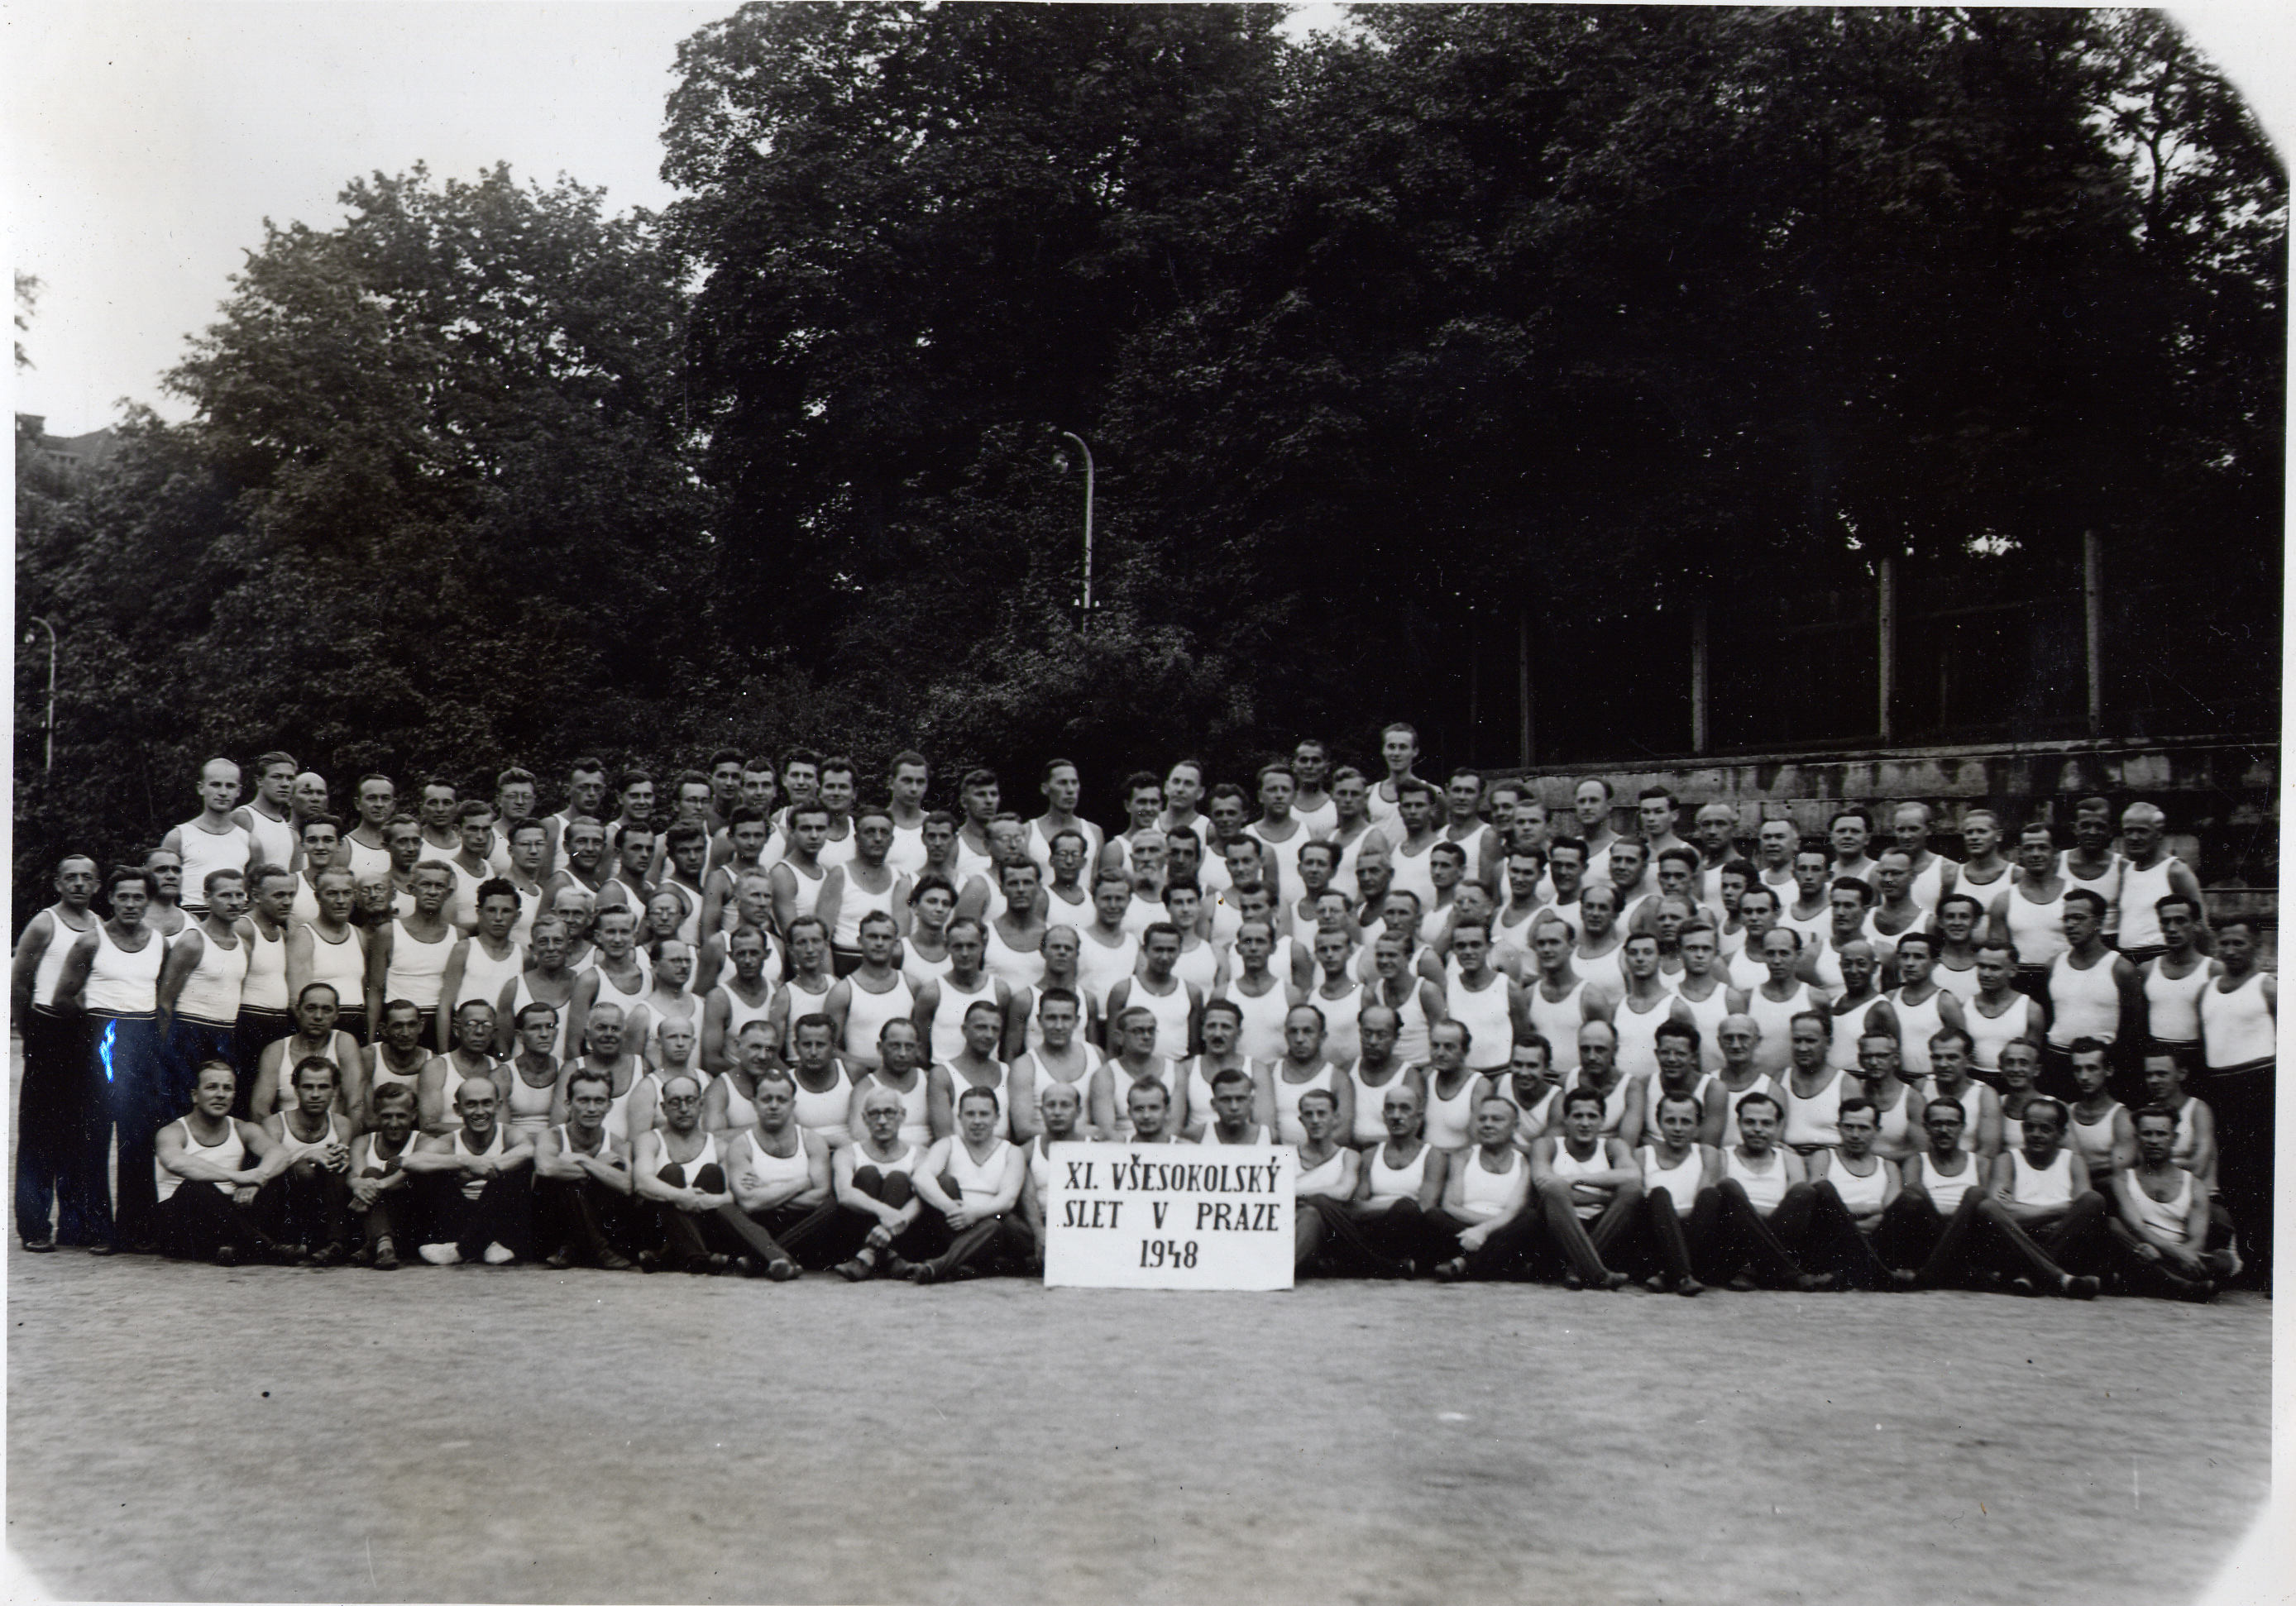
\includegraphics[width=0.9\textwidth]{img/31_muzi_cvicitele.jpg}
  \caption*{Cvičitelský sbor mužů 1948:\\zadní řada zleva: Dr. Svatoš, Reichrt,
  Dr. Fiala, Kofroň, Houdek, Čumrda, Němec, Válek st., Žáček, Malinský;\\
  střední řada zleva: Strachota, Ženíšek, Švejda, Pospíšil, Ing. Kvaček,
  Horák, Beneš, Horáček, Vaněk, Kočí, Válek ml., Šerák, Ferkl, Čejka,
  Tůma;\\sedící zleva: Mužík, Štěpánek, Doubek, Spurný, Jirák, Kodl,
  Mrklas, ?, Koubek;\\foto: archiv T.~J. Sokol Libeň}
\end{figure*}

\begin{figure*}[h!]
  \centering 
  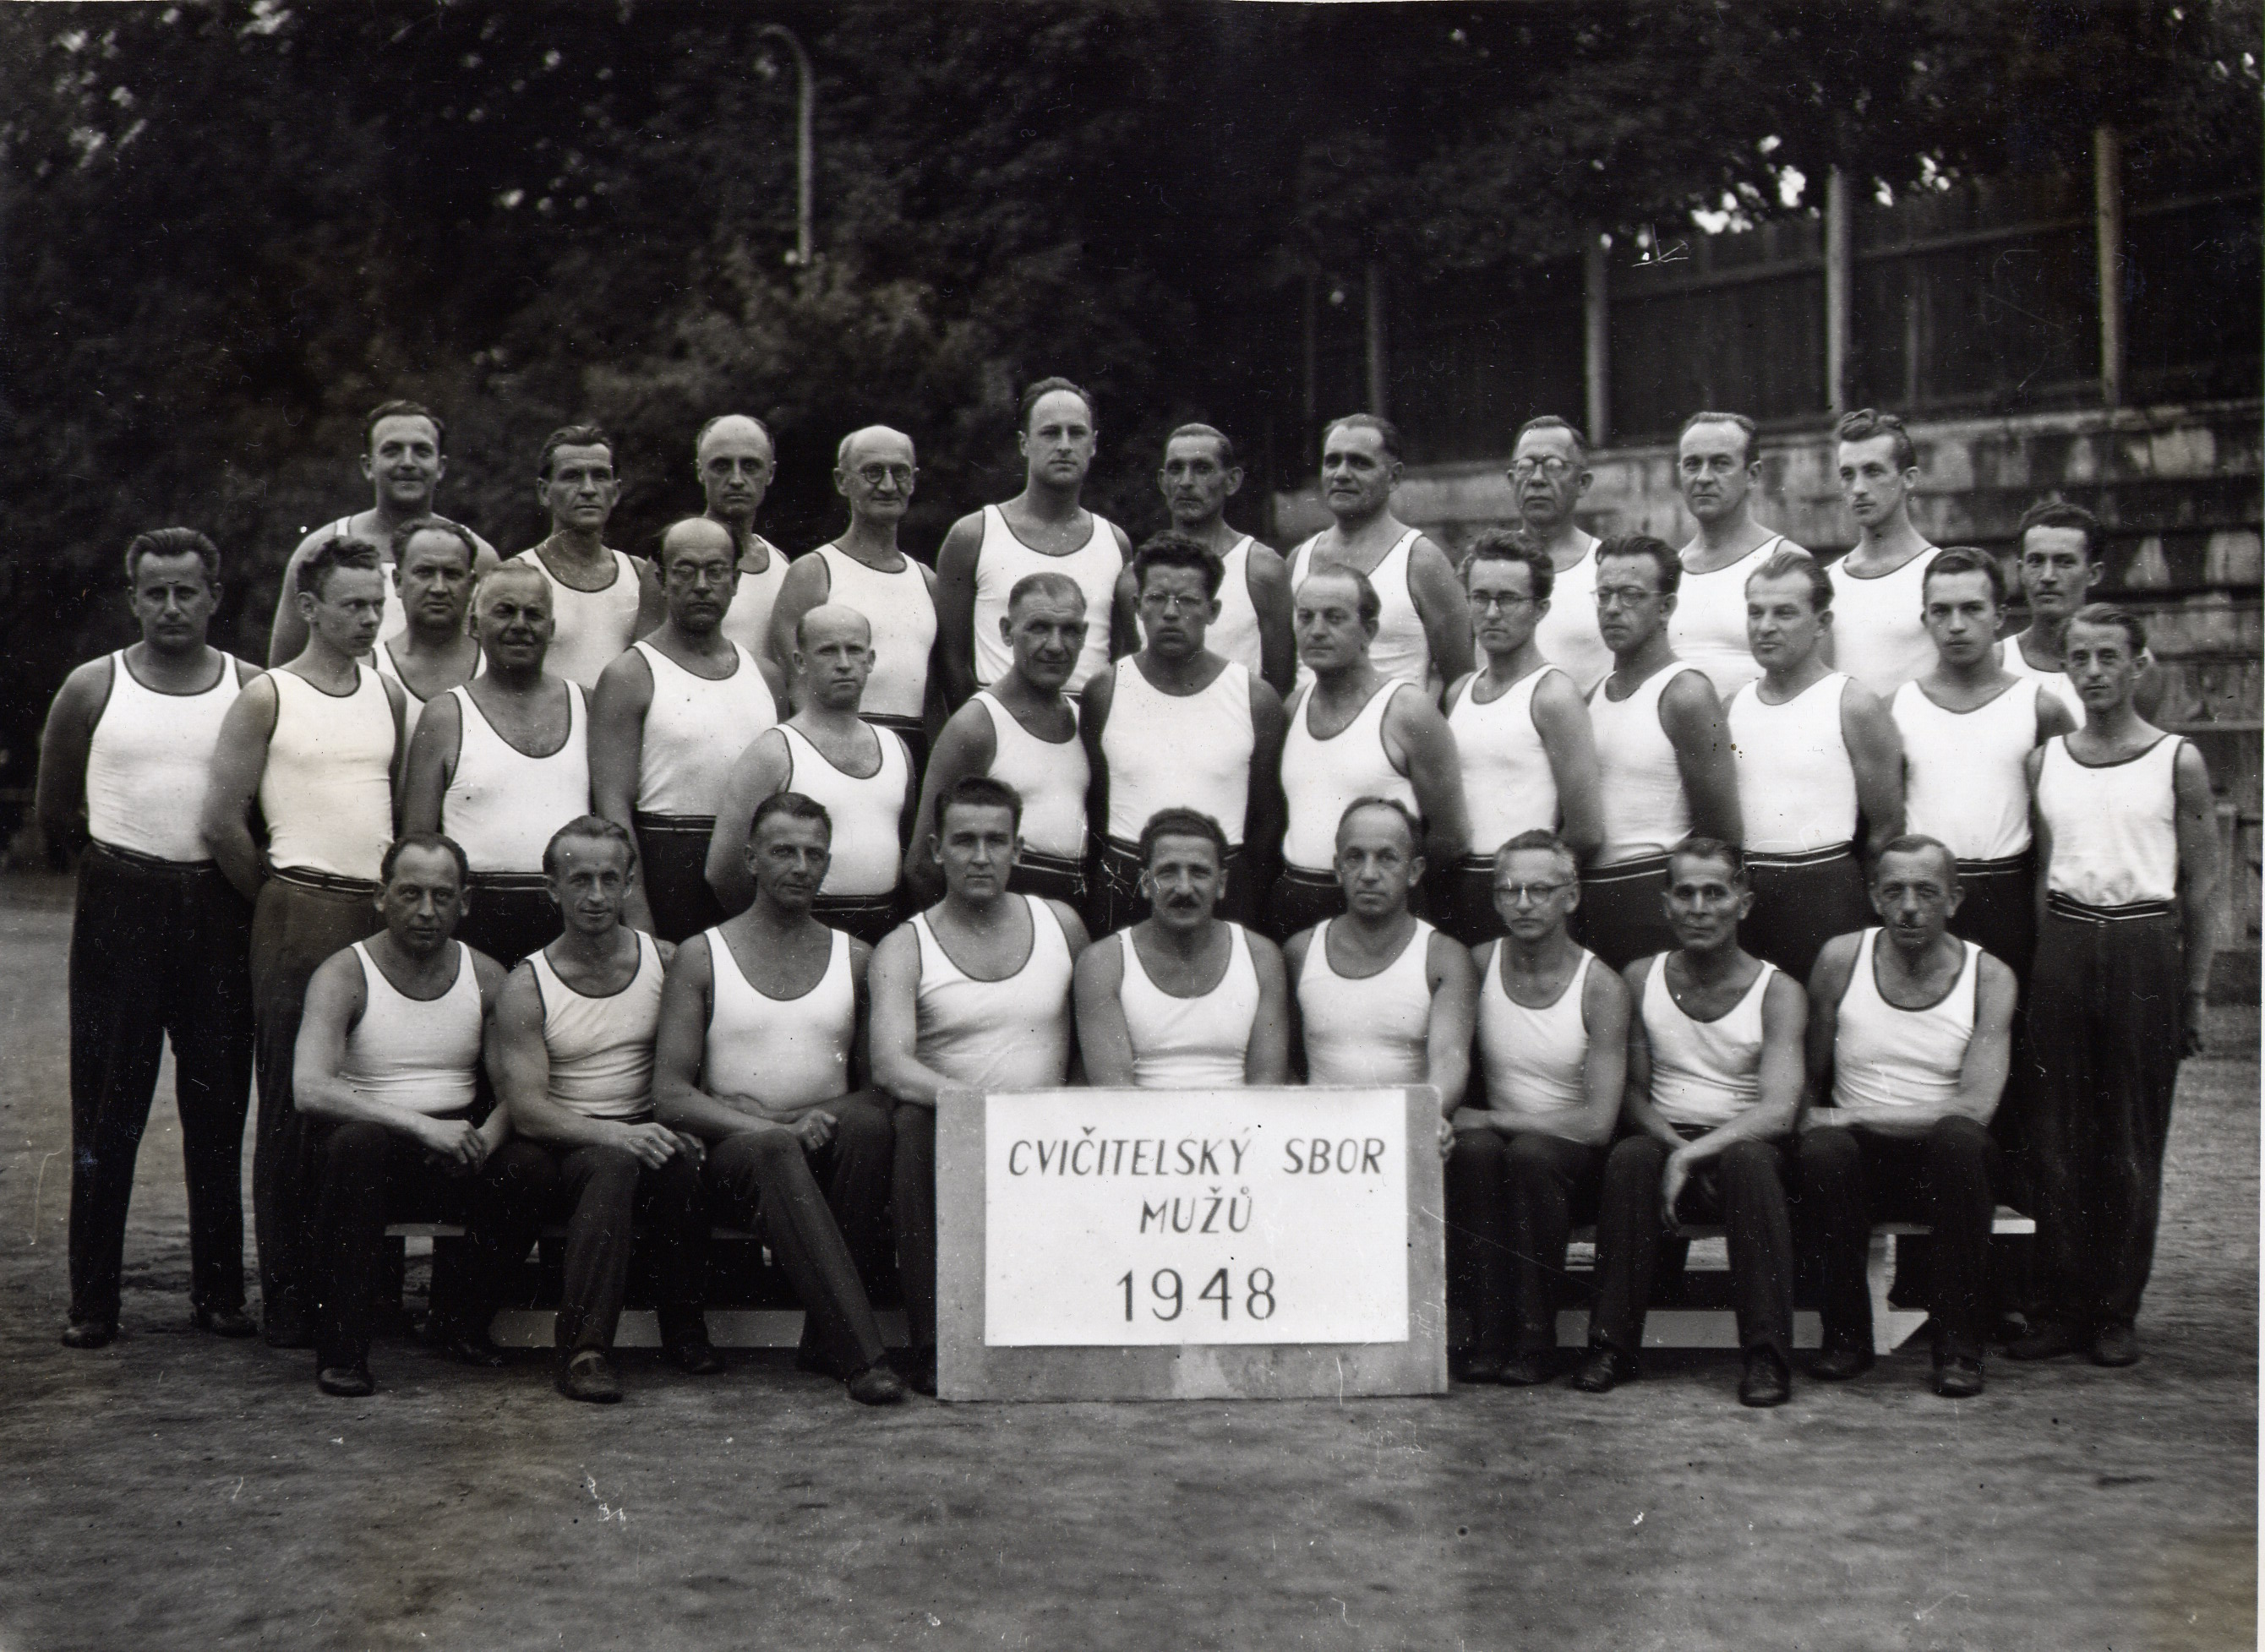
\includegraphics[width=0.9\textwidth]{img/32_muzi_cvicitele.jpg}
  \caption*{Muži 1948, foto: archiv T.~J. Sokol Libeň}
\end{figure*}
\vspace{\fill}

\section{Období let 1948--1968}

Před každým sletem byl značný příliv členstva i mládeže. Rok 1947 byl
v~tomto směru mimořádný. Členská základna ČOS vzrostla na jeden milion a
v~Sokole Libeň na 4\,201 duší. Žactvo, dorost i členstvo nacvičovali
sletové skladby ve dvou až třech oddílech -- tolik jich bylo.

\subsection{XI. všesokolský slet 1948 -- Strahov}

Deset let nechal na sebe čekat, zatímco předchozí slety se konaly vždy
po šesti letech. Slet začínal už v~roce 1946 ohňovým poselstvím, které
se šířilo pochodněmi z~Tyršova domu přes velikou hranici na Strahově do
sokolských jednot v~celé republice. Návrat byl štafetovým během
z~pohraničních měst do Tyršova domu, kam dorazili 27.~října 1947 poslední
z~80\,000 běžců na jedenácti tratích. Bylo to v~předvečer zahájení VIII.
valného sjezdu ČOS.

Zimní sletové hry členstva se konaly ve Vysokých Tatrách a zimní hry
dorostu v~Rokytnici nad Jizerou. V~té době probíhala v~Praze vládní
krize, která vyústila v~demisi vlády a vítězství komunistů (25.~únor
1948). Ti si vytvořili tzv. akční výbory v~podnicích, v~organizacích a
také v~ČOS i v~sokolských jednotách a začala "Očista" -- výměna
nepohodlných vedoucích. V~ústředí ČOS byl vyměněn starosta br. Hřebík,
náčelník br. Kavalír a řada činovníků. Za svoji náčelnici Marii
Provazníkovou se postavily ženy tak tvrdě, že prohlásily, že slet bez ní
nebude.

M. Provazníková, náčelnice ČOS o~té době říká: "Nadšení pohaslo po
únorovém puči a ještě více po abdikaci prezidenta Beneše. Má ještě smysl
dělat slet? Stačilo pár dní nové vlády, aby bylo jasno, že nastává konec
Sokola\ldots{} a přece jsme se rozhodli slet dokončit už proto, aby nebyly
zmařeny všechny oběti a úsilí již vynaložené a abychom se ještě sešli,
byl jen pro rozloučení. A~aby nám a zejména mládeži zůstala na Sokol
vzpomínka co nejkrásnější."

Slet se tedy konal. Byl největším (585\,000 cvičících) a nejkrásnějším ze
všech sletů. Kromě hlavních programů na ploše stadionu se konaly
nejrůznější závody a soutěže na hřištích a v~tělocvičnách atd. Např.
závody nářaďové, lehkoatletické, plavecké a vodácké, v~šermu,
v~lukostřelbě, ve střelbě z~malorážek, branné závody a závod Zborovský aj.
Konaly se soutěže ve hrách (házená, košíková, odbíjená), též
v~pochodovém zpěvu a v~recitacích (dorost) aj. Některých závodů se
zúčastnili i libeňští závodníci.

Žactvo z~Libně vystupovalo ve skladbách "Naše hračky", "Sokolské děti"
i v~prostných staršího žactva. Jaké byly starosti cvičitelů a cvičitelek
jen dopravit na Strahov na 350 žáků a přes 500 žákyň, tam se o~ně starat
a v~pořádku je zase přivést domů. A~kolik času a trpělivosti si vyžádal
vlastní nácvik?

Dorostenecká prostná nacvičil br. Ladislav Mrklas. Naši cvičili ve všech
hlavních sletových dnech. Působivá prostná byla přijata obecenstvem
s~velkým nadšením, zejména když si jednu část melodie hvízdali. Dále
překvapili diváky sletovou novinkou "Cvičební hodina v~přírodě".
Postavili v~několika minutách 1\,044 stanů-jehlanů do kruhových oblouků a
v~těchto stanových táborech předváděli obvyklý tábornický výcvik. V~obou
těchto sletových číslech a ještě ve cvičení s~plnými míči vystoupilo asi
180 libeňských dorostenců.

Dorostenky cvičily ve skladbách manželů Matějovcových "Bílé kroužky"
pod vedením sestry Blanky Holé a třikrát zaplnily celé cvičiště, pokaždé
jiné další cvičenky. Druhou skladbou dorostenek byla "taneční prostná
sestry Stázy Levé na národní písně". Tyto tance tady s~nimi nacvičila
sestra Věra Decastellová. V~úborech navržených Karlem Svolinským tančilo
4\,620 dívek a od prvních taktů jim patřilo celičké hlediště. V~obou
skladbách cvičilo z~Libně 230 dorostenek.

Ženy jako vždy byly zlatým hřebem sletu, ať to bylo ve
skladbě "Harmonie pohybu", nebo třicetitisícovém "Sletovém reji" či
v~cvičení nejvyspělejších cvičenek s~kužely. Tyto cvičenky ve čtvrtém
hlavním dnu nastupovaly v~dešti a již promoklé ze seřadiště. Na
rozblácené ploše stadiónu těžko hledaly značky a jejich postavy se
zrcadlily v~kalužích. Za tuto odvahu a kázeň byly odměněny takovým
potleskem a ovacemi, že opakovaly celé cvičení ještě jednou. A~bylo to
v~dějinách sletů poprvé, kdy celá skladba byla se souhlasem cvičenek
opakována. Bylo to slzavé a nejsmutnější rozloučení žen se sletištěm na
dlouhých 46 let. Z~Libně přivedla na Strahov 385 žen náčelnice Béda
Prokešová.

Muži zahajovali všechny hlavní sletové dny. Nastupovali za Sukova
slavnostního pochodu "V nový život". Prostná Františka Meduny nazvaná
"Věrni zůstaneme" byla věnována památce sokolských mučedníků z~let
1939--1945. Krásné verše Roberta Konečného recitoval Ladislav
Boháč. V~závěru při odchodu zpívali muži refrén písně:

\begin{center}
  
\textit{Bílá je čest a rudá věrnost k~smrti!}

\textit{Modrý klín víry vztek nepřátel zdrtí!}

\textit{Vítězná vlajko, květe slávy, štěstí,}

\textit{v~míru i bouři chceme tě věrně nésti!}
\end{center}

Zvláštním vystoupením mužů byla "Sokolská všestrannost". Bylo to
současné cvičení na 64 koních na šíř a 32 bradlech. Ve druhém a čtvrtém
hlavním dnu byla zvláštním vystoupením "Sokolská brannost" --
předvojenská příprava v~Sokole. Z~Libně cvičilo na XI. sletu 172 mužů
vedených náčelníkem Jaroslavem Jirákem. Libeňská Věrná garda cvičila ve
skladbě pro starší muže "Trojice s~dlouhou tyčí".

Sletový průvod členstva prošel Prahou ve IV. hlavním dnu dopoledne tj.
6.~července 1948. Zúčastnilo se ho 75\,000 mužů a žen v~krojích, 9\,000
hostů a přes 900 krojovaných jezdců na koních. Byl to tedy dosud
největší průvod. Procházel Václavským náměstím a končil na Staroměstském
náměstí, kde na tribuně seděl už nový prezident Gottwald a jeho nová
vláda i zahraniční delegace. Zatímco po celou cestu průvodu zněl jásot
pochodujících i obecenstva v~ulicích a ještě v~Pařížské ulici bylo
slyšet volání "Ať žije prezident Beneš!", kolem tribuny šli krojovaní
mlčky, se skloněnou hlavou nebo odvráceným pohledem. Tak projevil Sokol
nesouhlas s~novým násilně zavedeným režimem. Řada sokolů byla ještě ten
den zatčena a důsledky se projevily řáděním akčních výborů v~sokolských
jednotách. Vyloučeno bylo na 11\,000 členů. V~Libni to bylo 63 členů,
především činovníků a cvičitelů. Byl to starosta jednoty br. Štross,
náčelník Jaroslav Jirák, vzdělavatelka Helena Andrlová a řada jiných.

Po skončení slavnostních sletových dnů měly být na Strahově "Sletové
dožínky". V~autorském kolektivu byla řada vynikajících umělců,
režisérů, hudebních skladatelů aj. Nácvik se odbýval ústředně v~Tyršově
domě a jako rekvizita byl žlutý hedvábný šátek se vzorem od Mistra
Svolinského. Po změně prezidenta ženy odmítly v~nácviku pokračovat.
Poslední, tj. šestý den byl věnován československé armádě. Prostná
cvičení vojáků a ukázky bojového výcviku i seskoky padákem ukončily
nezapomenutelný XI. slet.

Vrátíme se ještě k~slavnému XI. sletu 1948 a trochu rozviňme to poslední
vystoupení žen s~kužely. Budeme citovat z~knihy sestry náčelnice Marie
Provazníkové "To byl Sokol" (vydáno roku 1988 v~Mnichově, str. 227):
"Silně ten den pršelo. Sestry byly promoklé, zkřehlé chladem, halenky se
jim lepily na těla; daly se však do cvičení tělem i duší. Slzy jim tekly
po tváři, zuby měly zaťaté, aby zabránily hlasitému vzlyku nad loučením
se sletem, se sokolstvím, co vneslo do jejich životů tolik krásy a tolik
štěstí. To nebylo cvičení, to byla bohoslužba a jejich zanícení a
rozechvění se přenášelo na tribuny. Čtvrt milionu diváků sledovalo
jejich pohyby se zatajeným dechem, pilo očima krásu, kterou vytvářely, a
svíralo bolestí nad jejich odchodem. Ve vzduchu visela otázka: Kdy se
zase sejdeme? A~co bude mezi tím? Proto to hrobové ticho ihned po
doznění hudby a pak ta bouře nadšení hrozící zbořit tribuny. Sestry
musely cvičení opakovat! Poprvé v~dějinách sletů se stalo, že se skladba
ihned po dokončení opakovala. Vynutili si to ovšem diváci. Byl to
poslední a nejsilnější dojem tělocvičné části sletu."

Tolik na dokreslení XI. sletu, který byl dosud největší a nejkrásnější a
po němž jsme čekali dlouhých 46 let na další XII. slet (1994).

\subsection{Pokus o~sjednocení tělovýchovy}

Po únoru 1948 vznikaly ve všech organizacích, a tedy i v~Sokole tzv.
akční výbory, které měly provést "očistu". Vylučovaly ze Sokola hlavně
vedoucí činovníky, které si členstvo svobodně zvolilo, a na jejich místa
dosazovaly "pokrokové" členy dle svého uvážení. Starostou ČOS se stal
br. Truhlář, náčelníkem br. Penninger. Náčelnicí zůstala sestra
Provazníková. Nové vedení ČOS nařídilo provést očistu ve všech
sokolských jednotách. U~nás stejně jako v~jiných jednotách, nenacházel
dvanáctičlenný akční výbor důvody k~vylučování. Tak se očistných akcí
ujaly tzv. "sokolské komise" při výborech Národní fronty. V~Libni
taková komise vyloučila ze Sokola nebo zbavila funkcí celkem 63 členů
pro "záporný postoj k~lidově demokratickému řádu naši republiky". Mezi
vyloučenými byl na prvním místě jmenován starosta Sokola Dr. Jiří
Štross, dále redaktor našich Zpráv K. Bíma s~manželkou, několik
cvičitelů, mezi nimi i br. Ladislav Horáček a také bývalý starosta
Dělnické tělovýchovné jednoty (DTJ) František Petráň i s~manželkou,
kteří do Sokola v~dubnu 1948 přistoupili. Mezi ženami to byly
vzdělavatelka sestra Helena Andrlová, Blanka Holá, vedoucí dorostenek,
cvičitelky Věra Decastellová a další. Vyloučených bylo 51 a zbavených
funkcí bylo 12, mezi nimi i náčelník br. Jaroslav Jirák, místonáčelnice
Marie Danihelková aj. Ve většině případů to mělo zlé následky i
v~zaměstnání, např. u~br. Jiráka.

Členstvo na vylučování reagovalo tak, že přestalo chodit do cvičení a ze
Sokola vystupovalo. Marně se nové vedení snažilo zvládnout situaci
ztíženou tím, že do Sokola musely vstupovat všechny tělovýchovné
organizace.

Košický vládní program z~roku 1945 již žádal sjednocení čsl.
tělovýchovy. Obnovení ČOS rozpuštěné v~roce 1941 bylo dlouho zdržováno
odporem komunistů, kteří chtěli hned sjednocení. Proto činnost ČOS mohla
začít teprve od ledna 1946. Všechny snahy ČOS o~sjednocení nikam
nevedly. Teprve poúnorový zákon z~března 1948 nařizoval povinné zapojení
všech tělovýchovných a sportovních organizací do jednotné organizace,
kterou byl Sokol.

V~Libni mělo do Sokola vstoupit celkem 15 takových organizací. Byly mezi
nimi 2 Dělnické tělovýchovné jednoty (DTJ), také Orel a dále libeňské
sportovní, hlavně fotbalové kluby, jako S. K. Meteor, Slavoj, Viktorie,
Čechie, Slovan a další (viz Zprávy 2/1948, str. 6 z~května 1948).
Většinou jen formálně byly připojeny, neboť většina funkcionářů nepřešla
a do nové práce se nezapojila, a tedy ani jejich členstvo ne.

{\sloppy V~roce 1949 se hledala posila členské základny v~dělnických
organizacích. V~Libni byly největším podnikem České loděnice, a tak
spojením s~jejich ROH byla jednota přejmenována na Sokol České loděnice.
Prvním předsedou byl Dr.~Václav Fiala, náčelníkem A. Novotný, náčelnicí
M. Pospíšilová.\par}

V~roce 1952 vznikají další závodní tělovýchovné jednoty a dávají si
jména: Dynamo, Spartak, Lokomotiva a pod. V~naší jednotě se ztrácí název
Sokol a vzniká Dobrovolná sportovní organizace DSO Spartak Libeň
Loděnice. Vlastnická práva na sokolský majetek (sokolovna, letní
cvičiště a obě horské chaty v~Krkonoších) přecházejí v~lednu 1954 na
Závodní radu skupiny ROH České Loděnice, n. p. (podle zákona č. 71/52
Sb). V~roce 1955 se tato nová jednota zúčastnila společně s~libeňskými
školami a ZV ROH Loděnice 1. spartakiády na Strahově. V~jednotách
vznikaly odbory Základní tělesné výchovy (ZTV).

V~roce 1957 vznikl Československý svaz tělesné výchovy (ČSTV). Jednota
se opět přejmenovala na T.~J. Libeň Loděnice. Z~majetkové podstaty ROH
byly podle zákona č. 68/56 Sb. vyňaty sokolovna a letní cvičiště.

Rok 1958 vykazuje veliký pokles členstva až na 1\,101, z~toho 232 žactva.
(Srovnáváme s~rokem 1945, kdy měl Sokol 2\,883 členů a koncem roku 1947
dokonce 4\,201 členů.) V~roce 1960 se konala 2. spartakiáda na Strahově
za účasti 135 žáků a žákyň, 96 žen a 18 mužů z~T.~J. Libeň Loděnice.
Slavné libeňské loutkové divadlo bylo předáno Osvětové besedě v~Praze 8.
Srncův sál, v~němž bylo umístěno perfektně vybudované loutkové divadlo i
se stupňovitým hledištěm, byl přeměněn pro potřeby nového oddílu
Umělecké gymnastiky (později moderní gymnastiky (MG)), který sem
přivedla Eva Foglová v~roce 1961. V~roce 1964 byl založen odbor
Kulturistiky, u~jehož zrodu stál Štěpán Fuczik.

Na letním cvičišti se začala v~akci "Z" přestavba bývalého kuželníku na
šatny se sprchami a klubovnou. Akce "Z" vždy znamenala hodně
dobrovolných brigádnických hodin, ale také dobrou spolupráci s~národním
výborem, s~odborem výstavby a hlavně s~finanční podporou. V~roce 1966
změnila Konference 17.~února název T.~J. Libeň Loděnice na T.~J. Meteor
Praha.

O~činnosti odboru ZTV vzniklém v~roce 1955 nejsou v~archivu Sokola téměř
žádné zprávy. Také v~Památníku stého výročí z~roku 1984 toho je velmi
málo. Teprve po roce 1968 nalézáme podrobné zprávy hlavně návratem
starých sokolů -- Věrné gardy do sokolovny.

\section{Libeňská sokolovna v~letech
1968--1984}

Dvacet roků chodili libeňští sokolové smutně kolem své sokolovny a jen
vzpomínali, kolik radostí jim od mládí tato milá budova poskytla. Teprve
celostátní obrodný proces vyvolaný Alexandrem Dubčekem a prezidentem
Ludvíkem Svobodou dával naději, že Sokol bude opět žít jako dříve.

\subsection{Pražské jaro roku 1968}

Politické napětí se uvolňovalo, a tak se již 6.~dubna 1968 sešel v~Praze
"Přípravný výbor Sokola", vydal provolání k~obnovení sokolské činnosti
a svolal nejprve pražské sokolstvo na Žofín (Slovanský ostrov) na den
21.~dubna 1968. V~Libni, jako v~jiných sokolských jednotách, se sešel
přípravný výbor Sokola a svolal Manifestační schůzi Sokola v~Libni na
úterý 30.~dubna.

{\sloppy Konala se v~zapůjčeném malém sále libeňské sokolovny a předcházela jí
schůze sokolských žen v~Karlíně. Schůzi v~Libni zahájil br. Jirák
přivítáním členů, zejména 93letého praporečníka br. Karla Panušky.
Hovořili: br. Jirák, sestry Danihelková, Andrlová a Věra Decastellová.
Obsáhlý referát o~Sokole přednesl br. Dr.~Jiří Štěpnička. Bratru Janu
Koubkovi bylo poděkováno, že tak svědomitě opatroval sokolské prapory a
celý bohatý archiv po celou dobu okupace až dodnes. Přítomným členům
byly rozdávány přihlášky do Sokola (ČOS). Průběh celé schůze byl
radostný a je zachycen na magnetofonovém pásku.\par}

V~Praze se pak konal ve výroční den Pražského povstání 5.~května 1968 na
Žofíně slavný a mohutný sjezd zástupců padesáti sokolských žup z~celé
republiky a dalších nadšených sokolů. Mnoho jich přišlo v~sokolských
krojích, ostatní se Suchardovým odznakem "Na stráž". Bylo tu na 3\,000
účastníků, do sálu se nevešli, a tak sledovali průběh sjezdu v~parku
z~amplionů, umístěných v~oknech budovy. Všechno se zdálo být dobré a
jasné, ale nebylo tomu tak dlouho. Politické uvolnění trvalo jen do 21.
srpna 1968, kdy nás v~nočních hodinách přepadla vojska Varšavské
smlouvy.

V~libeňském přípravném výboru Sokola (PV) byli zpočátku bratři Jirák,
Kodl, Štěpnička, Rusý, Andrle, Ladislav Svoboda, Ota Kačer a Josef
Hašek; za ženy sestry Věra Decastellová, Holá, Andrlová, Danihelková,
Vaňková a Kořínková. Že to neměli lehké zejména v~jednání o~zapůjčování
sálů aj. s~výborem TJ Meteor a tehdejším předsedou Hájkem, je patrno
z~mnoha zápisů.

Podmínky Meteoru byly pro nás nepřijatelné. Proto 11.~června se PV
rozhodl požádat Školskou správu ONV 8 o~souhlas k~propůjčování
tělocvičny ve škole Palmovka. Dohoda byla uskutečněna na dva dny v~týdnu
od 1.~září. Na schůzi 25.~června byl PV rozšířen o~br. Vajkrta a br.
Holého a bylo jednáno o~vydání nultého čísla Zpráv Sokola v~Libni.

V~těch měsících -- v~květnu a v~červnu -- se konalo mnoho schůzí PV jak
v~ČOS, tak v~Župách i v~jednotách. Důležité bylo setkání delegací ČSTV a
PV ČOS dne 23.~května a ustavení společných komisí; programové (Žižka a
Kavalír) a organizační (Šterc a Hobza) a také vzájemný slib, že si
nebudou narušovat vzájemnou činnost. Ale už v~červenci se v~tisku
objevují zprávy o~sporu mezi ČSTV a Sokolem. Na 5. plénu ČSTV došlo
ultimativním způsobem k~přerušení jednání. Dr. Hobza se ohradil
v~kinosále Tyršova domu dne 15.~července: "Chceme jednání rovný s~rovným a
žádné ultimatum!"

V~říjnu dostáváme důležité zprávy z~PV ČOS, že došlo konečně k~dohodě a
že byl ustaven Ústřední přípravný výbor tělocvičného svazu Sokol (ČsTS
Sokol). Předsedou se stal Dr. Šterc, místopředsedou Dr. Hobza,
náčelníkem Jiří Žižka, náčelnicí Eva Bémová, vzdělavatelem Dr. Hiller.
Obdobně má dojít k~splynutí PV Sokola (ČOS) a složek ZTV. Informovali
jsme o~tom TJ Meteor dopisem z~16.~října a navrhli setkání obou složek
23.~října v~sokolovně. Naše další schůze se konala 4.~listopadu v~Klubu
důchodců v~ul. Vosmíkových, byla rozšířena o~cvičitelské sbory a
připravila členskou schůzi Sokola ČOS na den 6.~listopadu 1968. Ta
rozhodla vstoupit do ČsTS Sokol v~TJ Meteor Praha. Na této schůzi,
zahájené a řízené br. Jirákem, byla uctěna vzpomínka na sestru Hanu
Decastellovou, která zemřela 27.~října 1968 ve věku 88 let. Byla
nejmladší zakládající členkou ženského odboru žen libeňského Sokola
v~roce 1898. Informace o~Sokole podali br. Štěpnička, ses. Decastellová a
hosté -- župní starosta br. Vágner a sestra Reindlová.

K~jednání s~TJ Meteor Praha došlo 11.~listopadu a bylo dohodnuto první
cvičení žen a mužů. Cvičení žactva a dorostu se předpokládalo až po
Novém roce. A~bylo tu tedy první cvičení ve čtvrtek 21.~listopadu 1968
-- ženy od 19.00 hodin, muži od 20.30 hod. ve velkém sále.

Ten den se také konala první beseda necvičícího členstva. Tu zahájil br.
Jirák, mluvil na ní župní vzdělavatel br. Růžek aj. Pozdravný dopis naší
nemocné vzdělavatelky ses. Andrlové přečetla Věra Decastellová. Bylo
odevzdáno 85 přihlášek i členských příspěvků a začalo se žít v~naší
sokolovně pod hlavičkou Československý tělocvičný svaz Sokol (Čs TS
Sokol).

"Pražské jaro 1968" nám otevřelo cestu do naší sokolovny, kam jsme
plných 20 let nevkročili. Jednání s~držiteli sokolovny -- s~výborem TJ
Meteor Praha i s~odborem ZTV (Základní tělesná výchova) byla obtížná a
zdlouhavá, takže teprve 21.~listopadu 1968 mohlo členstvo začít cvičit
v~sokolovně. Náčelník ZTV Ing.~Václav Ďoubal přivítal naše muže a
náčelnice ZTV Miloslava Štěpánková naše ženy-sokolky. Jedněm ani druhým
se to moc nelíbilo -- každý ale musel něco ze svého slevit. Ustavující
schůze nového odboru Sokol se konala 3.~února 1969 a byl zvolen výbor
v~tomto složení:
% TODO chce Míla odstranit mezeru?
\medskip
předseda: Josef Kříž (1926)

místopředseda: Ing. Jiří Polanecký (1934)

náčelník : Ing. Václav Ďoubal (1933)

místonáčelník: František Kodl (1909)

jednatel: Josef Rusý (1922)

vzdělavatel: Miroslav Hokův (1929)

metodik: Dr. Jiří Štěpnička (1924)

náčelnice: Věra Decastellová (1919)

hospodář: Otakar Kačer (1915)

zdravotník: MUDr. Alena Nevařilová (1925)

soutěže: Otakar Zima (1936)

tělovýchovná vystoupení: Jindřich Vondrášek (1935)

bez funkce: Miroslav Tůma (1921), Jiří Pospíchal (1935), Alena Vávrů (1934)

Z~původního výboru ZTV zůstali: Polanecký, Ďoubal, Vondrášek a Zima.

\medskip

První členská beseda 7.~března 1969 byla věnována prvnímu prezidentovi
T.~G. Masarykovi a již 19.~března zahájil metodik Dr.~Jiří Štěpnička
třicetihodinový kurs pro cvičitele. Také již v~březnu byly pořízeny
jmenné seznamy členstva původního ZTV i přistoupivšího ČOS. Vykazují 124
mužů a 321 žen, tedy celkem 445 dospělých. Příchodem 270 sokolů vzrostl
počet členstva odboru Sokol o~61\,\% a dále rostl. TJ Meteor Praha udává
k~20.~června 1970 celkem 1\,995 členů ve 12 oddílech a v~tom byl
nejpočetnější Sokol 955 členů, tj. 47,9\,\%.

Přestože byl příliv členů veliký, ve cvičení se to neprojevilo.
Celoroční průměr ve cvičení mužů byl jen 12,9, u~žen 37,75, žáci i
žákyně průměr 25. Rozdělení cvičebních dnů nebylo dobré. Muži cvičili
v~pondělí a čtvrtek, žáci úterý a pátek, cvičitelé žáků tedy nechodili do
cvičení mužů (4 dny v~týdnu). Velmi pozdní začátek cvičení mužů od 20,30
hod. (po cvičení žen --⁠⁠⁠⁠⁠⁠ 19,00--⁠⁠⁠⁠⁠⁠20,30 hodin) byl asi hlavní příčinou malé
návštěvnosti. Hlavní výbor Meteoru vzal mužům hodiny ve velkém sále,
určil jim cvičení jen v~lodích, později v~Srncově sále. Tam pro
nedostatek nářadí se cvičení zvrhlo jen na fotbálek.

Velmi dobře si vedli cvičitelé žáků. Na městský přebor ve sportovní
gymnastice 9.~4. 1970 na Zlíchově připravoval žáky cvičitel Václav
Kilián. Družstvo mladších žáků obsadilo 1. místo (z~9 družstev) a
v~jednotlivcích získal 1. místo Aleš Krotil, 2. místo Václav Pernecký.

Mnoho dalších dobrých akcí vykazoval výbor odboru Sokol v~"Analýze
činnosti 1968--1970", která má 8 stran a kterou si vyžádal hlavní výbor
Meteoru. Na mimořádné společné schůzi obou výborů 7.~12. 1970 se snažil
výbor Sokola obhájit svoji činnost, ale marně. Vše bylo předem
rozhodnuto, analýza nebyla k~ničemu. Předseda hl. výboru Dr. M. Hájek
prosadil "zastavení činnosti výboru Sokola s~okamžitou platností" a
vyzval k~opuštění místnosti.

Bezpráví, hrubost a ponižování byly ještě znásobeny článkem "Rozlet
libeňských sokolů" v~Rudém právu z~29. a 30.~12. 1970. Redaktorka M.
Hojerová v~něm, na základě informací předsedy Dr. M. Hájka, očernila
výbor Sokola, jak nejlépe dovedla. Nejhůř byl napaden předseda Josef
Kříž a náčelnice Věra Decastellová. Výbor Sokola protestoval. Poslal
doporučené dopisy hlavnímu výboru TJ Meteor, žádal revizní komisi
Meteoru o~přešetření. Od ní dostal po urgenci za 6~týdnů neurčitou
odpověď, dále žádal o~pomoc Městský výbor Sokola, stěžoval si i na OV
KSČ. Naši osmistránkovou "Analýzu činnosti" snad nikdo ani nečetl,
natož aby porovnával úspěchy Sokola s~nedostatky, k~nimž se výbor
přiznával. Zkrátka: doba již Sokolu nepřála.

V~roce 1971 odbor Sokol jen živořil pod vedením předsedy Josefa
Blumensteina a náčelníka Jindřicha Majera (oba KSČ). Náčelnici odbor
celý rok neměl, až teprve 11.~října potvrdil hl. výbor do funkce Věru
Haufovou. Na výroční schůzi 16.~12. 1971, svolanou předsedou
Blumensteinem, se sešlo 44 členů, ale hl. výbor nedovolil její konání,
že nebyla dostatečně připravena. Konala se tedy až 20.~ledna 1972 za
účasti 59 členů. Byl zvolen nový výbor odboru Sokol, který s~malými
změnami řídil činnost až do roku 1989. Zvoleni byli: předseda prof. Dr.
Miroslav Hauf, místopředsedkyní Marie Kodlová, náčelníkem Jindřich
Majer, místonáčelníkem František Kodl, náčelnicí Věra Haufová,
místonáčelnicí Alena Vávrů (naše pobočka ve škole na Invalidovně),
zapisovatelkou Miluška Rusá, hospodářem Ludvík Holý a pro styk
s~necvičícím členstvem Jarmila Šandová (Procházková).

Tento výbor přinesl mnoho nového a dobrého do tělocvičné činnosti odboru
Sokol. Tak již v~roce 1972 zavedl novinku: cvičení rodičů a dětí (R+D)
podle prof. Jany Berdychové. Byli jsme mezi prvními v~Praze. V~tomtéž
roce jsme pro naše cvičitele uskutečnili 11~lekcí cvičení na trampolíně.
Vedl Luboš Novotný, účast 12~mužů i žen. Koncem roku odbor podal
přihlášku o~titul "Vzorný kolektiv".

Věrná garda, oddíl necvičícího členstva, začínala svoji činnost také již
v~roce 1972. První beseda se konala ve Filipově síni 22.~března, účast
36. Na příští besedě (26.~dubna 1972) promítal své barevné diapozitivy
z~Paříže předseda Dr.~Hauf. 45~účastníků si vyslechlo i nové francouzské
šansony. Třetí beseda nazvaná "Zemi milované" byla věnována památce K.
H. Máchy. Dr.~Mirek Vaněk v~roce 1973 hovořil o~olympiádě v~Mnichově,
koncem roku Dr. Fr. Bulánek vzpomínal na starou Libeň. U~kolébky těchto
besed stál František Kodl, později Adolf Peťule. V~roce 1974
připravovali oba společně cyklus pěti besed, zaměřených na 90. výročí
založení Sokola v~Libni (1884). Vybírali v~archivu fotografie,
šibřinkové pozvánky, kresby v~Památníku cvičitelského sboru a obrázky ze
sletových památníků a z~těch pořídili ofotografováním černobílé diafilmy
a ty na besedách roku 1974 promítali a komentovali. Tak získali trvalý
kádr našich starších členů -- pamětníků a dali pevný základ nynější
"Věrné gardě", o~níž se ví nejen v~Praze, ale v~celé republice, že je
nejčilejší a doopravdy sokolskou. Od roku 1975 je vedena "podpisová
kniha" na besedách a je tedy přesná evidence o~počtech účastníků. Za 22
roků činnosti je průměrná návštěva 45 osob. Máme i kroniku Věrné gardy,
i samostatnou "Obrazovou kroniku". Jsou v~nich zachyceny kulturně
poznávací vycházky, výlety do přírody i autobusové zájezdy.

\subsection{Období 1972 až 1984}

V~novém devítičlenném výboru odboru Sokol v~TJ Meteor Praha, zvoleném
20.~1. 1972, bylo 7 dobrých, zkušených a hlavně velmi pracovitých
sokolů. Manželé Haufovi a Kodlovi, Miluška Rusá a Ludvík Holý, později i
Jindra Vajkrt -- to byli hlavní činitelé, kteří dokázali vyvést odbor
Sokol z~kritických situací. Na jedné schůzi se výbor usnesl, že všichni
budou své zprávy předkládat písemně. Pečlivě se kontrolovalo plnění
celoročního plánu, a když se začalo soutěžit o~titul "Vzorný odbor",
dbalo se na plnění všech dobrovolných závazků. Na tiskopisech se
znamenala docházka do cvičení u~všech složek a koncem cvičebního roku se
odměňovali nejlepší. Dobře spolupracovaly cvičitelské sbory. Jejich
společná schůze se konala každý měsíc a předcházela schůzi výborovou.
Věra Haufová dbala na dodržování pořádku a byla iniciátorkou mnoha
dobrých a úspěšných činností. O~schůzích cvičitelského sboru žen máme
v~archivu hodně zápisů.

Soutěžení žactva a dospělých patřilo do kritérií pro získání titulu
"Vzorný". Soutěžilo se ve sportovní gymnastice o~přebor jednoty i
vyšších celků (oblasti i města) a také o~odznak zdatnosti (OZ) i dětský
odznak zdatnosti (DOZ). Dospělí muži i ženy soutěžili zejména ve hrách
odbíjená, košíková). Za něco byly diplomy, za něco odznaky. O~odznacích
"Zlatá Praha" bude dále ještě psáno ve zprávě o~turistice mládeže i
dospělých.

V~našem archivu máme hodně zajímavého materiálu o~tělocvičné činnosti,
o~výletech a autobusových zájezdech. Vybíráme některé zajímavosti. Tak
např. v~oddílu nejmladšího žactva, který vedla Františka Pášová, se
konala 24.~2. 1975 zimní soutěž, kde získal 3. místo a 18,5 bodů náš
nynější starosta -- Jiří Novák. Tehdy mu bylo 5 let. Jinde čteme, že
v~docházce za září až prosinec 1977 byl 10.~nejlepší sedmiletý žák Jiří
Novák (28 hod. = 87,5\,\%). Na obvodní soutěži SG 28.~3. 1978 v~Karlíně
se umístil Jiří Novák na pátém místě počtem 27 bodů, tj. 90\,\%.

V~kategorii starších žáků se umístil Roman Kolář na 2. místě 36,7 bodů,
tj. 91,75~\%. V~docházce se vyznamenal Roman Kolář v~roce 1976/77, kdy
byl nejpilnějším a po 6 měsíců měl 100\,\% docházku, celkem 62 cvičebních
hodin.

Školení cvičitelů a cvičitelek byla věnována také velká pozornost.
V~roce 1976 absolvovali školení IV. třídy dorostenci: Zdeněk Lauschmann
(17) a Martin Halík (15). V~následujícím roce pak: Josef Řezníček (29),
Aleš Krotil (19) a Josef Srnský (15). Průkaz cvičitele III. třídy
získali v~roce 1978 Řezníček, Lauschmann a Halík. Na školení IV. třídy
bylo přihlášeno v~roce 1976 celkem 15 mladých cvičenek, např. Jindra
Hovorková. Někteří další působí dnes již v~jiných jednotách, např.
Zdeněk Lauschmann (Zlíchov), Martin Halík (Vinoř).

Tělocvičné akademie se konaly každoročně. Zvlášť pečlivě se připravovaly
ty k~90. a 95. výročí (1974 a 1979) založení Sokola v~Praze-Libni.
Mimořádně významné byly oslavy 100. výročí v~roce 1984. Na těchto
oslavách velmi záleželo hlavnímu výboru TJ Meteor Praha, protože v~jeho
znaku pod zelenou hvězdou bylo použito letopočtu 1884, tedy vzniku
Sokola, zatímco SK Meteor byl založen roku 1896, tedy o~12 let později.
Oslavy probíhaly od jara. V~dubnu se konala první zkušební Tělocvičná
akademie věnovaná oslavám. Deset čísel programu bylo dílem našich
autorů, tedy původních. Hostem byly ženy TJ Tesla Žižkov, zřejmě sokolky
a předvedly v~dobovém cvičebním úboru prostná žen na VI. sletě 1912. To
bylo v~naší sokolovně.

V~divadle S. K. Neumanna v~Libni (dnešní divadlo Pod Palmovkou, kde
v~hostinci U~Deutschů byla založena 26.~října 1884 Tělocvičná jednota
Sokol Libeň) v~jeho krásném sále se konala slavnostní akademie -- 15.
října v~17:30 hodin. Bohatý program uváděl herec divadla pan Jiří Havel.

Program slavnostní akademie ke 100. výročí založení jednoty se
skládal z~následujících vystoupení:
%TODO co takhle?
\smallskip
Cvičení dříve a dnes -- ml. žáci, autor F. Kodl

Když se míč schová v~síťce -- ml. žákyně, vedoucí J. Hovorková

Cvičení na třech hrazdách -- st. žáci TJ Slavoj Praha 7, autor Dr.
Kašák (Slavoj také slavil 100. výročí)

Mládí -- radost -- pohyb -- st. žákyně, ved. J. Hovorková

{\sloppy Mládí v~Moderní gymnastice -- dívky, ved. Eva Foglová (komponováno k~25.~výročí MG) \par}

Pódiová skladba s~lentou (\pozned{se stuhou, pozn. ed.}) -- dívky MG,
ved. Eva Foglová

\smallskip
Po přestávce byly udělovány slavnostní plakety zasloužilým tělovýchovným
pracovníkům. Plakety převzaly i někteří starší sokolové, např. bývalý
starosta Sokola Dr. Štross, náčelník Jaroslav Jirák, loutkář Jar.
Beránek, archivář Adolf Peťule, matrikář Ludvík Holý a jiní. Mnoho
vyznamenaných bylo z~TJ Meteor a také mnozí činovníci našeho odboru,
tehdy již odboru ZRTV (Základní a rekreační tělesné výchovy).

Tělocvičná část slavnostní akademie pokračovala:

\medskip
Aerobik -- ženy MG, ved. Eva Foglová a Tamara Janů

Radost z~pohybu -- ženy ZRTV, ved. Věra Decastellová

Rytmus mládí -- mladí cvičitelé, autoři naši hosté Luboš Čapeka a
Dana Rádová (vítězná skladba ze soutěže pódiovek 1982 v~Žilině)

\medskip
Slavnostní schůze se konala 24.~října 1984 ve velkém sále libeňské
sokolovny za účasti mnoha čelných představitelů obce, tělovýchovných i
jiných organizací. Také zde byli vyznamenáni další pracovníci
v~tělovýchově, rozdávány pamětní listy a vlaječky.

O~přestávce si návštěvníci slavnostní schůze prohlédli výstavu ke 100.
výročí, uspořádanou ve Filipově síni libeňské sokolovny ve 2. patře. Ze
zachovalého archivu tam snesli bratři Peťule, J. Valenta, F. Kodl,
sestry Decastellová, Kodlová, Šulcová, Holá aj. mnoho cenných památek.
Výstava trvala celý týden a vidělo ji hodně návštěvníků i žactvo školy
Na zámečku.

K~dokreslení období stého výročí musíme ještě napsat o~činnosti Moderní
gymnastiky a oddílů Jóga a Kardio, o~turistických oddílech ml. žactva a
JILMu a o~bohaté činnosti Věrné gardy. Členové těchto oddílů mají veliký
podíl na tom, že libeňská jednota patřila a stále patří mezi ty nejlepší
v~Praze.

\begin{center}
\textit{Potud končí vyprávění br. Peťuleho o~vzniku a činnosti T.~J. Sokol
Libeň; o~období let 1984--1989 vypráví dále br. František Kodl.}
\end{center}

\section{Období 1984--1989}

\begin{center}
  \textit{Sepsal br. František Kodl (1909--1998)}
\end{center}

\noindent
K~oslavám v~jubilejním roce 1984 byl vydán hezký Památník stého výročí
založení Tělocvičné jednoty Sokol v~Praze-Libni. Největší část připravil
archivář a vedoucí Věrné gardy bratr Adolf Peťule. Sportovní části a
konečnou úpravu do tisku provedl redaktor Tomáš Svoboda. Byl to již
třetí Památník libeňského Sokola (k~25., 50. a 100. výročí). V~Památníku
je oceňován vzestup kvality cvičení v~odboru Sokol po roce 1972, kdy se
přihlásil do Soutěže o~titul "Vzorný odbor". Soutěžila tehdy celá
jednota, všechny oddíly i všechna družstva. Počet členů a hlavně mládeže
rostl, docházka do cvičení se lepšila. V~roce 1984 byla průměrná
návštěva v~jedné cvičební hodině tato:

\medskip
\textbf{žactvo:}

rodiče a děti 10 párů

předškolní žactvo 16

mladší žáci 21

starší žáci 29

starší žákyně 16

dorostenci 4

dorostenky 5


\medskip
\textbf{členstvo:}

muži -- zákl. gymn. 7

ženy -- zákl. gymn. 17

muži -- kondiční gymn. 13

ženy -- Invalidovna 19

ženy DG na Žernosecké 86

Jóga, muži a ženy 12

KARDIO, muži a ženy 48

\medskip

\noindent
Byl nedostatek cvičebních prostorů, takže mladší žáci a mladší žákyně
cvičili společně ve velkém sále, někdy se tam ani nevešli. Podobné
problémy mělo starší žactvo a dorost. Přesto se jména libeňských dětí
objevovala v~soutěžích mezi prvními. Cvičitelé nechyběli na žádném
cvičitelském srazu ani školení. V~jednotě probíhalo dlouhodobé školení,
které vedla metodička Dáša Horáčková. V~soutěži o~titul "Vzorný odbor"
byl získán III. stupeň roku 1973, II. stupeň 1978, I. stupeň 1983.
Bronzová plaketa k~I. stupni získána roku 1986. Stříbrnou plaketu k~I.
stupni by býval odbor dostal v~roce 1990. Vyznamenání Zásluhy o~rozvoj
tělesné výchovy II.~stupně získal již v~roce 1985.

Každoročně se konaly Dětské karnevaly a Dětské dny spojené s~autobusovým
zájezdem a také Mikulášská nadílka. Odbor pořádal tělocvičné akademie,
na kterých se objevovala vždy nová čísla našich mladých cvičitelů. Do
soutěží pódiových skladeb bylo posíláno až 5 skladeb. Uveďme alespoň tu
nejpopulárnější z~roku 1989, skladbu Jindry Štefkové a Josefa Řezníčka
s~názvem "Pruhovaná". Dostala tehdy druhou cenu.

Měli bychom si připomenout alespoň jména tehdejších žáků, kteří se
objevují v~sokolovně i dnes, již jako cvičitelé, např. Jiří a Tomáš
Novákovi, Vladislav a Pavel Voráčovi, Jan Kolář, Filip Kadlec, Aleš
Kafka, Jan Hora, Radek Zeman, Tomáš Novotný a jiní. Už tenkrát pracovali
jako cvičitelé František Kodl, Zdeněk Lauschmann, Martin Halík, Roman
Kolář, Josef Srnský, Josef Řezníček, Aleš Krotil, Martin Vetengl a jiní.
Cvičitelky: Věra Decastellová, Věra Haufová, Janešová, Anna Kavinová,
Marie Kodlová, Hovorková-Štefková aj.

\subsection{Turistické oddíly
žactva}

V~osmdesátých letech se zrodily dva turistické oddíly. Turistický
kroužek mladšího žactva (TK1) založili a dlouho vedli manželé Kodlovi.
Vrcholné období kroužku začalo v~roce 1980, kdy na získání odznaku
"Zlatá Praha" bylo obětováno 11~zimních sobot (leden--březen) a
průměrná účast byla 22 osob. Následovalo Léto v~Posázaví (\(3\times\)) a potom
Hřebeny Brd (\(4\times\)), kde již pomáhali mladší cvičitelé Lauschmann a Halík.
V~lednu 1981 žactvo poznávalo Románskou Prahu (\(8\times\)) a Gotickou Prahu
(vedla J. Besperátová). Dobře motivované byly výlety žactva spojené
s~četbou Jiráskových pověstí. Na 7 výletech "Po stopách starých pověstí
českých" byla účast 22 až 36 osob. V~jubilejním roce 1984 byly velmi
úspěšné vycházky po Praze 8 "Poznáváme své město". Bylo jich 9
s~průměrnou účastí 24~osob. Vycházky měly dvě části: kulturně poznávací,
ke které byl rozmnožen dvojlist (na textech spolupracoval br. A.
Peťule), druhá část vycházky byla rekreační -- obyčejně někde na louce
nebo v~Areálech zdraví -- hry.

Každoročně se také v~červnu konaly autobusové zájezdy dětí (např. \(5\times\) do
Českého ráje). Prázdninové soustředění mladšího žactva bývalo
v~chatičkách TJ Meteor v~Chřenovicích na Sázavě. O~bohaté činnosti obou
turistických kroužků by se dalo ještě mnoho psát, zejména o~pestrosti a
nápaditosti programů práce s~dětmi, ale to snad při jiné příležitosti.

\clearpage
\subsection{Turistický kroužek starších žáků a dorostenců (TK2) =
JILM}

\pozned{O~oddílu JILM je podrobněji pojednáno ještě v~textech jeho
vedoucích Z. Lauschmanna, J. Nováka a J. Přecha dále, pozn. ed.}

Programy vycházek mladšího žactva byly stále náročnější, a tak bylo
nutno ustavit kroužek starších žáků a dorostenců. U~samého zrodu stál
Zdeněk Lauschmann a 1.~února 1982 se narodil turistický oddíl JILM
(\textit{JILM je zkratka ukrývající zakázaný název "Junáci indiánské lesní moudrosti", pozn. ed.}). K~víkendovým výpravám každý třetí týden
přibyly ještě středeční schůzky v~klubovně. Na schůzkách se připravovaly
výpravy a žáci se učili čtení map, práci s~buzolou, uzlování, vzdělávali
se nenásilně v~akcích Děd Vševěd, Všeuměl, Jazykohrátky, Pamatovák a
jiné úkoly, které si Zdeněk vymýšlel. Dost času bylo vždy na hry,
soutěže a písničky při kytaře. Výpravy bývaly jednodenní, v~létě
dvoudenní s~přenocováním v~přírodě nebo v~turistické noclehárně. Chlapci
se učili znát přírodu, květiny, rostliny, stromy, hledat červený tis i
strom jilm, jehož list je ve znaku oddílu. Nachodili hodně kilometrů
pěšky, dělali výpravy i na kolech. Na výpravách byly oblíbené dlouhodobé
bojové hry, stejně jako každoroční zimní hra "Vyzvědači" v~ulicích
Starého Města. Stanové tábory si Jilmáci stavěli na zelené louce a často
měnili místa. Zkusili i Putování na Slovensku. Nebáli se ani brigád
v~okolí sokolovny a na udržování "Chráněných území na Praze 8".
V~osmdesátých letech spolupracovali s~vedoucím Roman Kolář, Josef Srnský,
Jiří Beneš a jiní.

\subsection{Věrná garda}

Věrná garda je oddíl krásného přátelství a pravého bratrství, jak si to
představoval zakladatel Sokola a první starosta Jindřich Fügner. V~roce
1984 měla naše Věrná garda za sebou již 9 roků bohaté činnosti a 72
besed s~průměrnou účastí 42,3 osob na jedné besedě. Prvních 49 besed
bylo věnováno cyklu přednášek "Znáš tu zem líbeznou? Krásy
Československa -- slovem i obrazem". Na 50. besedě se objevil nový
cyklus přednášek nazvaný "Daleké cesty". V~roce 1984 to byl Split a
ostrov Hvar (Josef Valenta) a od různých přednášejících: Normandie,
Kavkaz, Mexiko a jiné země. Dvě besedy v~tom jubilejním roce byly
věnovány promítání diafilmů pořízených z~archivních dokumentů již k~95.
výročí. Výklad podal archivář br. Peťule.

V~rozmnožovaných měsíčních programech Věrné gardy bývají oznamovány
čtyři druhy akcí, kromě besed, návštěva výstav nebo kulturních památek
v~Praze, celodenní výlety do okolí Prahy a autobusové zájezdy do
vzdálených míst. Vynikající vedoucí mnoha zájezdů byla Františka Pášová,
která však 13.~4. 1984 zemřela. Posledním jejím zájezdem byl zámek
Frýdlant a Lázně Libverda v~roce 1982. Z~celodenních výletů uvedeme
cyklus největší: "Putování kolem Prahy za 24 dní". Vedeni Ludvíkem
Holým a Františkem Kodlem jsme našlapali celkem 112 kilometrů a 20
účastníků získalo odznak 100 jarních kilometrů. Jejich věkový průměr byl
73,05 roků. O~všech akcích je v~archivu bohatá obrazová dokumentace a 7
kronik Věrné gardy.

\subsection{Jóga}

Jóga, oddíl zdravotního tělocviku, byl zaveden již v~roce 1981.
Vedoucími byli obětaví manželé Jeřábkovi a také Věra Haufová. Průměrná
návštěva cvičení byla zprvu 10--12, v~letech 1986 až 1989 vzrostla až na
18. Cvičilo se nejdříve v~malém sále zvaném též Badmintonový (dnes Alšův
sál podle velikého Alšova obrazu). Sál byl na jógová cvičení příliš
chladný, proto se přešlo do Srncova sálu, kde se cvičí dodnes (\pozned{již
tomu tak není, oddíl klasické jógy v~současnosti naše jednota nemá,
formuje se však zatím neformální oddíl akrojógy (párové akrobatické
jógy) pod vedením sester Kolářových, pozn. ed.}).

\subsection{Zdravotní oddíl Kardio}

Zdravotní oddíl KARDIO cvičil také jen jednou týdně a v~roce 1984 měl
v~šesti skupinách průměrnou návštěvu 48,4. Byl založen a řízen MUDr.
Jarmilou Winterovou z~kardiologického oddělení OÚNZ v~Praze 8. Od března
1981 se stali všichni členy odboru ZRTV. Na každém cvičení byl přítomen
lékař a zdravotní sestra. Společnou rozcvičku vedla Markéta Ladová,
studující na lékařské fakultě. Cvičení bylo několikrát přerušeno a
cvičenci si měřili tepovou frekvenci a museli vysadit při dosažení
předepsaného maxima. Podle lékařského vyšetření byli rozděleni do skupin
podle dovolené zátěže od 50 do 150 wattů. Počet cvičících kardiaků stále
vzrůstal až na průměr 64,3 v~roce 1987. V~březnu roku 1988 byl celý
oddíl převeden do zdravotního odboru TJ Meteor Praha.

Sametová revoluce v~roce 1989 ukončila činnost odboru ZRTV a všichni
dobří a "věrní" pracovníci přešli do Sokola, obnoveného v~Libni 28.
března 1990, v~den výročí narození Jana Amose Komenského.

\section{Sokol za komunismu (?!)}

\begin{center}
\textit{Vzpomínka na dobu Františka Kodla, sepsal RNDr. Zdeněk Lauschmann (v~Libni od roku 1976 jako dorostenec)}
\end{center}

Není to nějaký omyl? Sokol a komunismus -- vždyť to vůbec nejde
dohromady! A~přece to není omyl, jen je třeba malého vysvětlení.
Samozřejmě -- slovo Sokol nebylo tenkrát nikde napsané, ani nemohlo být.

Ale co je to vlastně ten Sokol? To jsou přece nějací lidé, nějaká
činnost a nějaká myšlenka, ne? Pak ovšem odbor Základní a rekreační
tělesné výchovy tělovýchovné jednoty Meteor Praha byl sokolský
skrznaskrz.

Nepochybně to byla zásluha manželů Kodlových, kteří po roce 1968 odbor
vedli spolu s~dalšími zapálenými spolupracovníky. Většina z~nich
vyrostla ve skutečném, předválečném Sokole a měla v~sobě to, čemu se
říká sokolský duch. Je to především ryzí lidství, zní tam však silně
také obětavost jedince pro celek, ale nefanatická, je to elán i
bojovnost, ale neagresivní, a hlavně je to radost ze všeho krásného a
dobrého. Tyto vlastnosti z~oněch lidí vyzařovaly stále a všude --
v~tělocvičně, na hřišti, ve městě i v~přírodě -- a celá léta jemně a
přitom účinně formovaly všechny, kdo se do bohaté činnosti libeňské
jednoty zapojili.

Když potom, po roce 1989, mohl být Sokol v~Libni obnoven i podle jména,
tak vlastně nebylo co řešit -- odbor ZRTV až na několik jednotlivců
přešel jako celek do ČOS. Cvičitelé i činovníci prostě jen pokračovali
ve své práci a nováčci ve výboru, sokolským duchem odchovaní, přirozeně
navázali na své moudré předchůdce. A~kluci? Ti beztak odjakživa "chodili
do Sokola", tak jen vyměnili červené trenýrky za modré a jelo se dál.

\section{Ženy v~libeňském
Sokole}

\begin{center}
  \textit{Na začátky cvičení žen a své působení v~libeňském Sokole vzpomíná dlouholetá náčelnice Milada Věra Decastellová (1919--2014).}
\end{center}

K~základní zprávě o~historii a vzniku naší jednoty a k~její činnosti za
uplynulých 120 let je nutno přidat neodmyslitelnou účast žen. Od žákyň
počínaje, až k~těm nejvyššího věku a k~těm, které s~námi nepřestaly
sympatizovat. Takže můj příspěvek se bude týkat hlavně ženských složek,
jako důležité součásti celá jednoty.

Jistě mi bude odpuštěno, že některé pasáže si čtenář přečte v~obou
příspěvcích. Můj celý život je příliš svázán se Sokolem, abych neuvedla
rodinné vzpomínky mých rodičů a sourozenců i své vlastní.

\begin{figure*}[h!]
  \centering 
  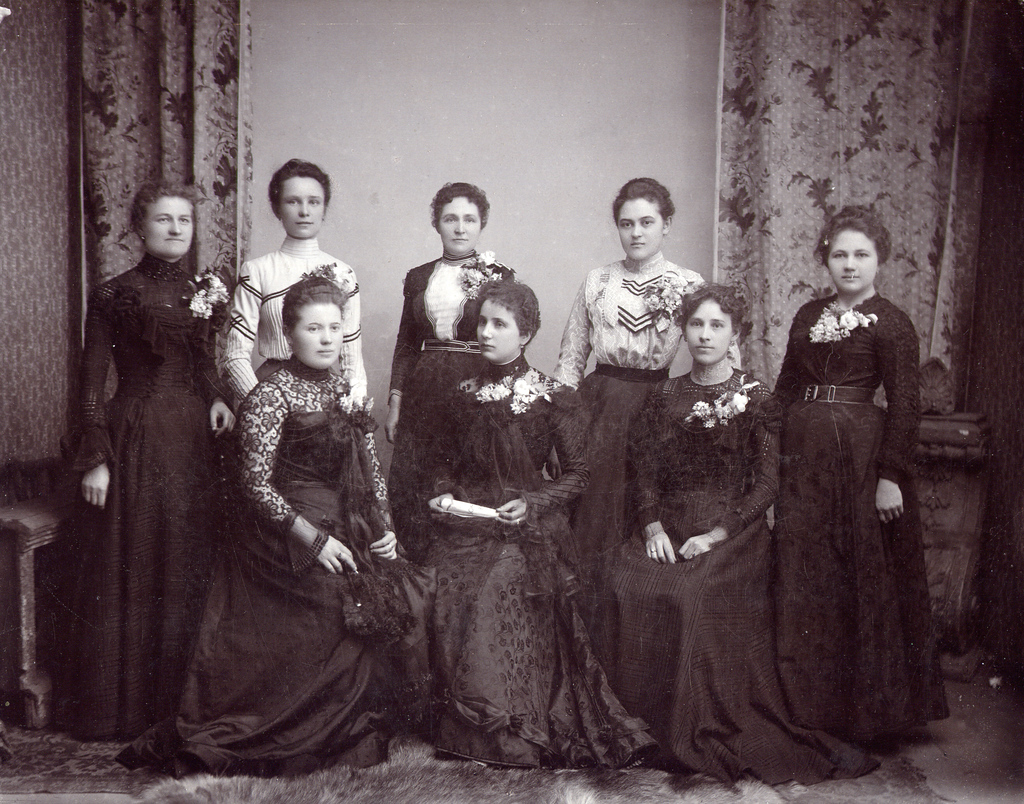
\includegraphics[width=0.9\textwidth]{img/33_zakladajici_zeny.jpg}
  \caption*{Zakládající výbor odboru žen libeňského sokola (1899), foto:
  archiv T.~J. Sokol Libeň}
\end{figure*}

Zakládající výbor odboru žen byl ustaven již v~roce 1898 a na fotografii
z~roku 1899 můžeme vidět všechny jeho členky. Ještě ani ne osmnáctiletá
je tam moje maminka. Jinak jsou to vesměs manželky členů jednoty a
vážených libeňských občanů. První náčelnicí byla zvolena paní Růžena
Vocetková, tehdy si ještě sestro neříkaly. Na dobových fotografiích si
všimněme oblečení, utváření cvičebních úborů a hlavně počtu žákyň, podle
tehdejší módy oblečených do stejné podoby s~dospělými. Významný byl rok
1893, kdy paní a dívky věnovaly libeňskému Sokolu nádherný dvoustranný
prapor se stuhami, který můžeme vidět ještě dnes, pietně uchovávaný
v~archivu (\pozned{jeho repliku můžete vidět na našich akcích, pozn. ed.}).

\begin{figure*}[h!]
  \centering 
  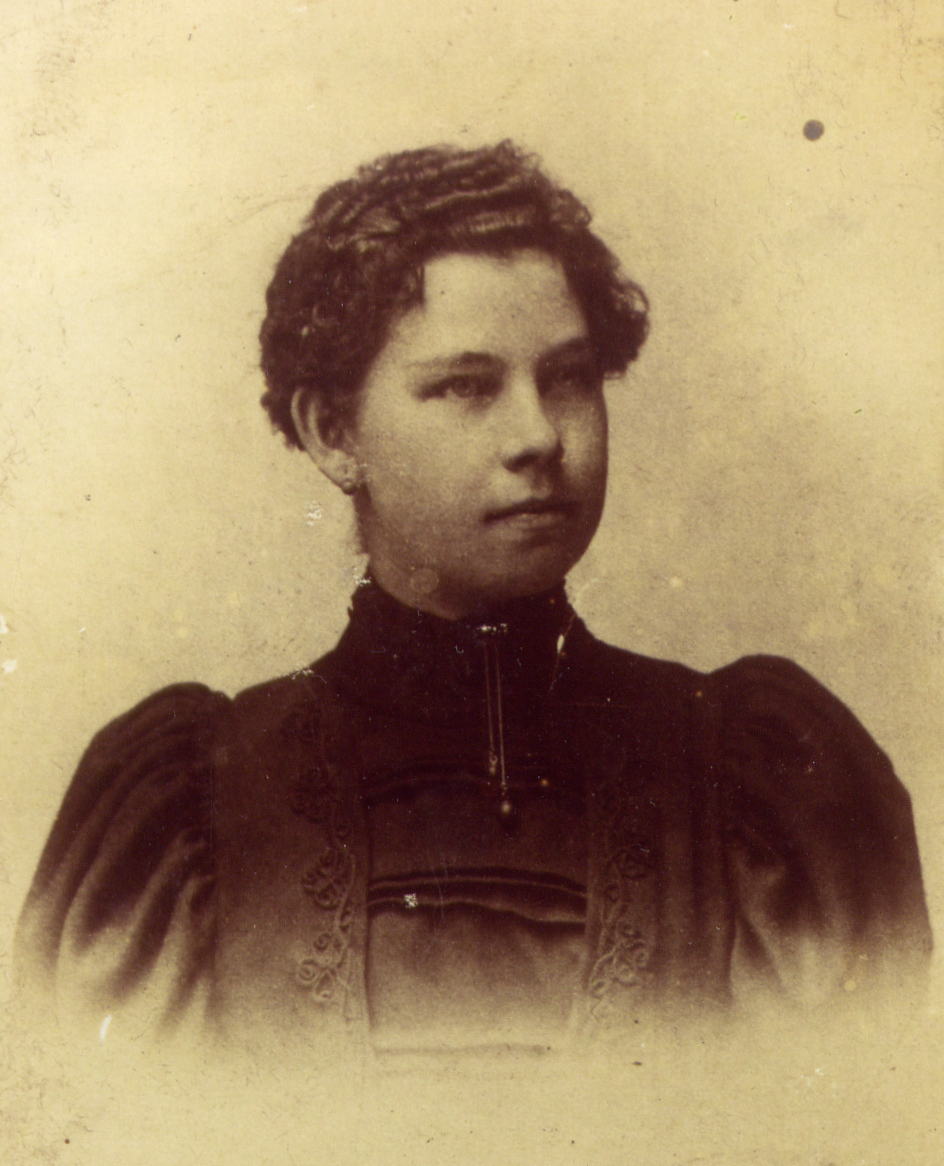
\includegraphics[width=0.6\textwidth]{img/34_vocetkova_nacelnice.jpg}
  \caption*{Růžena Vocetková, první náčelnice Sokola Libeň (1899), foto:
  archiv T.~J. Sokol Libeň}
\end{figure*}

Přelom století přinesl v~roce 1901 již IV. všesokolský slet, kdy se
poprvé svým cvičením na veřejnosti předvedly i ženy. Libeň se v~tu dobu
ukázala veřejným cvičením na místě zvaném Pánkovo pole. Víte, kde to
bylo? V~místech, kde dnes projíždí metro, dříve železnice, prostor mezi
ulicemi Na Žertvách a Novákových, jak vidíme na dobových fotografiích (str. 27). % ref: veřejné cvičení
Počty ženských složek se po sletech, od roku 1901 a 1907 zvedaly a byly
to hlavně mladé ročníky. V~roce 1909 bylo péčí tehdejšího starosty
bratra Filipa a celého výboru rozhodnuto o~stavbě vlastní budovy
sokolovny. Po dohodě se zastupitelstvem obce Praha VIII bylo přistoupeno
ke stavbě. Požadavkem bylo, že součástí sokolovny budou i městské lázně.
Za pouhých 9 měsíců, s~finančním přispění obce, byla sokolovna postavena
a 14.~srpna 1910 slavnostně otevřena.

V~přípravách na poslední předválečný slet v~roce 1912 se sokolovna
cvičícími jen hýbala. V~jedné hodině střídavě cvičilo cca 30 žen, 18
dorostenek, ale už přes 80 žákyň (fotografie to jasně dokládá).

\begin{figure*}[h!]
  \centering 
  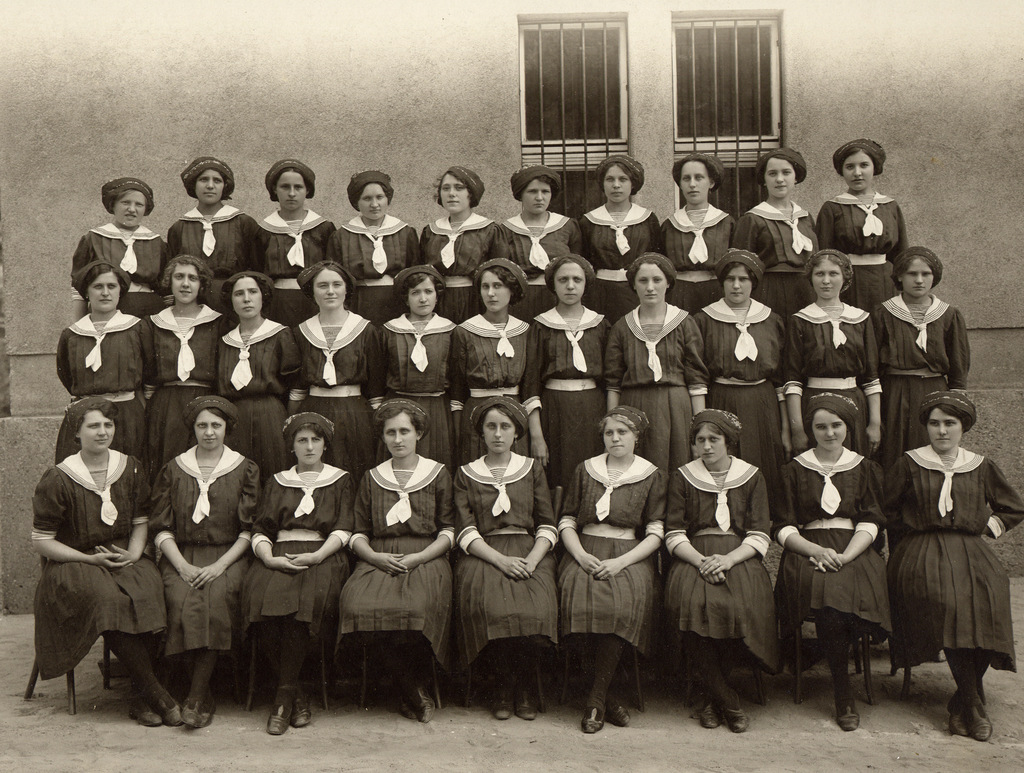
\includegraphics[width=0.9\textwidth]{img/35_zeny.jpg}
  \caption*{Ženy 1912, foto: archiv T.~J. Sokol Libeň}
\end{figure*}

Bohužel první světová válka tvrdě zasáhla do všeho dění českého života a
tím i do Sokola. Muži narukovali, ženy byly přinuceny se samy starat
o~rodinu a navíc mnohé pracovaly na válečných úkolech. V~sokolovně byl
zřízen vojenský lazaret, jehož život máme rovněž na mnoha fotografiích.
Dokonce v~místech, kde dnes stojí garáže (\textit{nyní zde jsou parkovací
místa, pozn. ed.}), se pěstovaly brambory pro pacienty.

Rakousko-Uhersko skončilo a první roky naší republiky posvětil i Sokol.
Byly zřízeny sokolské obranné hlídky, které působily do doby, než byla
utvořena armáda Československé republiky. Jako doklad uchováváme
červeno-bílou růžici jako odznak těchto útvarů.

Hned v~roce 1920 byl uspořádán VII. všesokolský slet a je známo, že
venkovské jednoty dovezly tolik potravin, že o~jídlo měla postaráno celá
Praha. Pochopitelně Libeň se zapojila nebývalým počtem cvičících.
Všimněme si v~mém příspěvku ženské účasti: 115 žen, 170 dorostenek, 314
žákyň! Co k~tomu dodat!

Tehdejší život se celoročně soustřeďoval v~krásné nové sokolovně,
o~které se dovídáme i v~jiných příspěvcích. Po válce se nutně změnilo
využívání volného času. Přibyl zájem o~moderní pojetí cvičení, což
znamenalo více využívat přírodu.

Vracíme se k~pořádání výletů, vzniká odbor pobytu v~přírodě a odbory
tzv. prostého tělocviku. Jsou to míčové hry a atletika. Je nutno
vybudovat cvičiště. Po různých jednáních a přesvědčování se ustavila
v~roce 1923 za vedení bratra Bessera "Stará garda", která na sebe tuto
povinnost vzala a nastala práce. Opět se uplatnily ženy ve velkém počtu
175 žen a dorostenek při odkopových pracích. Konečně v~roce 1924 byly
práce dokončeny a červen t. r. se pochlubil cvičením všech složek
jednoty. Fotodokumentace ukazuje první kopáčské práce na nerovném
terénu, vyrovnání cvičební plochy hřiště, stavbu krásné brány, domku pro
sokolníka a mnoho záběrů z~bohatého života na cvičišti v~dalších letech.

\begin{figure*}[h!]
  \centering 
  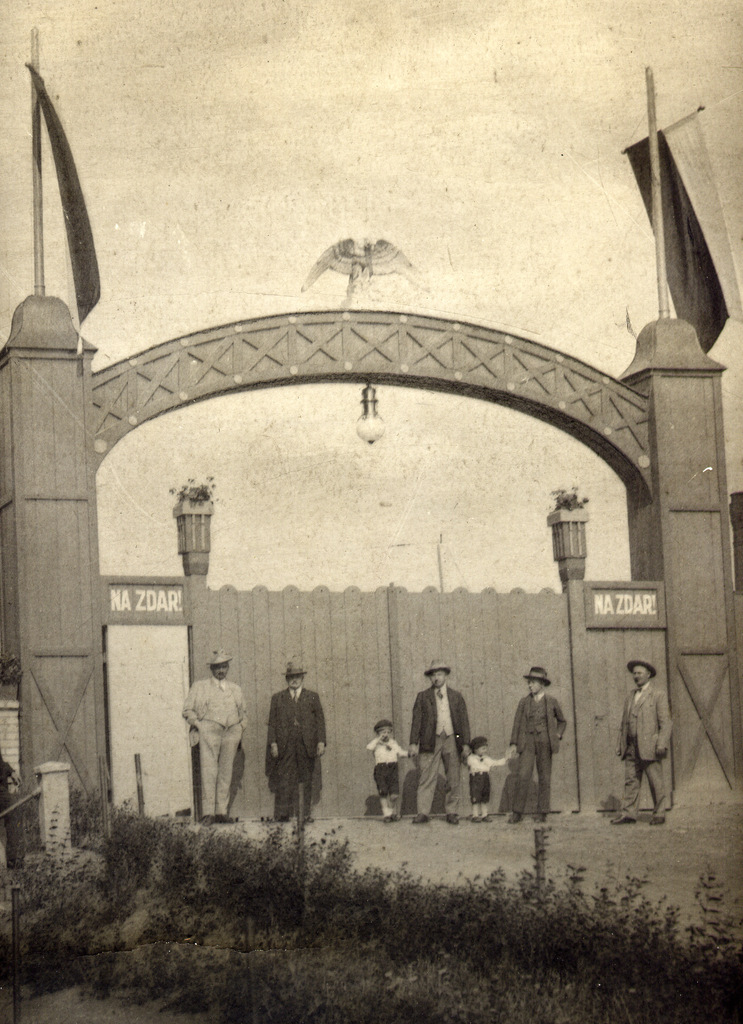
\includegraphics[width=0.6\textwidth]{img/36_brana_cviciste.jpg}
  \caption*{Brána letního cvičiště, foto: archiv T.~J. Sokol Libeň}
\end{figure*}

Protože firma Grab, které patřil z~větší části pozemek, žádala 1 mil.\,Kč
za prodej, byl dohodnut pronájem, který trval 10 let; až pozemky
převzala pražská obec. V~roce 1933 byl uskutečněn převod do vlastnictví
celého prostoru cvičiště a mohly začít další úpravy.

Letní cvičiště se vedle sokolovny stalo eldorádem sokolské mládeže i
dospělých. Volejbal, házená, určitý čas i tenis, dětský koutek, kuželník
a hlavně všechny disciplíny atletiky. Startovní bloky, doskočiště,
atletický ovál, konstrukce na kruhy a hrazdu i vhodné místo pro bradla.
Blízkost sokolovny byla při změně počasí velkou výhodou. Letní cvičiště
se stalo rovněž svědkem velkých veřejných vystoupení. Jednota zde
pořádala vedle různých krojových slavností také veřejné předsletové
ukázky cvičení, v~mezidobí se zde konaly župní slety a všechno to bylo
libeňskou veřejností velice ceněno. Průvody Libní byly vždy jejich
součástí.

A~tak zatímco léto jsme prožívali na cvičišti, po podzimním turnaji
v~házené, kdy se opět uplatnily ženy-sportovkyně, připravila se sokolovna
na posvícenskou veselici (svátek sv. Havla), jak měla obec Libeň ve
zvyku. Téměř pravidelně se zde vypíjel vyhraný pohár z~házené. A~nastal
čas stěhování členů Sokola do tělocvičny, i když na cvičišti se ještě
proháněli různí vytrvalci. Připravovala se akademie, mikulášská a velice
oblíbený Kryšpánek cvičitelských sborů. Jak šel čas, každý rok končil
Silvestrem, začínal Novým rokem a už se nacvičovaly šibřinky. Opravdová
půlnoční scéna ladila s~rázem šibřinek a rovněž výzdobou sokolovny.
Půlnoční scény byly téměř vždy prací žen, z~nichž je nutno vyzvednout
jméno naší dlouholeté vzdělavatelky ses. Andrlové. Zimní plesové
radovánky se odbývaly v~sokolovně ve dvou sobotách a ukončily je ještě
dozvuky před příchodem jara.

Jarní besídka ukázala, co se děti přes zimní měsíce naučily ve cvičení,
ke Dni matek poděkovaly maminkám za vychování. Naše cvičitelky měly
velkou zásluhu na správném vývoji sokolského žactva, což mohli vždy
potvrdit lékaři při pravidelných prohlídkách dětí. Celý kolotoč se rok
co rok opakoval, vždy v~trochu jiné podobě a s~jinými nápady a také
s~jinými dorůstajícími dětmi. Nácviky na to všechno dění byly vždy
náročné, ale radostné a každý si považoval za čest být vybrán
k~účinkování. Jaká chuť nacvičovat, hlavně v~době předsletové i u~těch,
kteří se během roku moc nesnažili. V~roce 1932 při IX. všesokolském
sletě jsem již byla starší žákyně a patřila mezi ty, které se pyšnily
účastí na něm. Předcházelo mu v~květnu okrskové cvičení všech složek
v~Měšicích a župní slet žactva v~Libni. Jen naše jednota tam přivedla
kolem 300 cvičenců všech věkových stupňů. Předsletového veřejného
cvičení na našem letním cvičišti se zúčastnilo téměř 900 cvičenců.

Nácviky se odbývaly při pianu, v~té době nebyly žádné desky a kazety, a
tak je nutno se zmínit o~našich obětavých a hlavně neúnavných
pianistech. U~mužů to byl při cvičení bratr Kvaček, u~žen sestra
Šilingerová, která pro nás dokonce složila pochod "Sokolky jdou".
Nechala jsem ho oživit na kazetu. Obětavým a trpělivým klavíristou byl
pro nácviky všeho druhu bratr Česta Kondelík. Náš "Kondelíček", jak
jsme si ho překřtily, byl ochoten přijít kdykoliv a doprovázet nás při
zkoušení, poradit s~hudbou i tanečním projevem, což jsme ocenily hlavně
v~době poválečné.

Vraťme se však do roku 1924, v~roku 50. výročí trvání naší jednoty.
Pamětní tisk z~té doby nám mnoho napoví a my jen žasneme, co vše se nám
nabízí -- jako program oslav -- podle dochované pozvánky. Současně jsme
si připomněli, že již 10 let nám slouží letní cvičiště.

Období let po IX. sletu (1932) bylo pochopitelně plné různých sokolských
událostí. Množství besídek, akademií, jiných vystoupení a jejich bohatou
kulturní náplň si ověřujeme nejen na obrazových materiálech, ale také
v~různých písemných dokladech, jako jsou zápisy ze schůzí náčelnictev,
pořadatelského sboru, loutkářů a všech dalších oddílů. Kupříkladu velký
význam mělo odhalení pomníku JUDr. Jana Podlipného v~roce 1935 a v~roce
1937 zájezd Pražského pětižupí na Slovensko, jehož jsme byli jako
jednota silnou skupinou. Rovněž důležitý byl téhož roku zájezd k~naší
menšinové svěřence v~Trmicích (dnes část města Ústí nad Labem), kde
fašistický živel velice sužoval naše české občany, hlavně sokoly a jiné
národní organizace.

Působení ženských složek je v~těchto a všech dalších letech už tak
spjato s~činností celé jednoty, že není třeba oddělovat jejich úlohu.
Ženy zastávají různé činovnické funkce, mají též rozhodující vliv
v~náčelnictvu a ve správním výboru a zastupují jednotu v~mnoha vyšších
složkách župy a ČOS. Do tohoto období spadá hlavně příprava na poslední
předválečný slet v~roce 1938. Naše jednota obsadila mnoha cvičenkami
celostátní prostná a mimořádně zajímavý rej pro téměř 30\,000 žen.
Zvláštní vystoupení pro vyspělé cvičenky bylo vystoupení s~červenými a
bílými míči. Ten červený s~mnoha podpisy našich i zahraničních sokolů
jsem celá léta schovávala, než přece jen podlehl letité zkáze.

Následné válečné roky nás bohužel všechny rozloučily. Tak jako dřívější
slety, měl i tento svou sletovou scénu. Nutno tedy připomenout, že
v~roce 1938 měla přiléhavý název "Budovat a bránit" a jejím autorem byl
náš přední člen a světoznámý loutkář Dr. Jan Malík. V~počtu 5\,000
účinkujících jsme i my libeňští měli své zastoupení, mezi nimi jsem byla
i já. Tento hold republice se stal, bohužel, i rozloučením s~naší
národní svobodou.

Tento X. všesokolský slet v~roce 1938 patří k~tomu nejkrásnějšímu období
sokolské práce. Byl však už předzvěstí nejtragičtějších následků okupace
naší vlasti. Začala druhá světová válka, naši nejlepší odcházeli za
hranice, vznikl domácí odboj a následovaly těžké postihy všech vrstev
našeho národa. Již od příchodu nacistů se tvořily odbojové skupiny,
mnohdy velice naivně pojaté a snadno se stávaly oběťmi gestapa. Vznikaly
ovšem i velice dobře organizované vojensky řízené skupiny, z~nichž se
uplatnil nebývalou měrou odboj sokolský. Libeň jako místo vybrané
k~atentátu na říšského protektora Heydricha tak měla řadu těch, kteří
položili život za naši svobodu. Jejich jména jsou na věčnou paměť
uchována na čelném místě naší sokolovny. NEZAPOMÍNEJME!

Toužebně očekávaný konec šestiletého utrpení nastal a Sokol se dal opět
do svobodné práce. Ukázala se výhoda blízkosti letního cvičiště, kde se
hned v~květnu 1945 organizovala setkání všech bývalých členů jednoty a
nových zájemců. Ihned začalo vyklízení sokolovny, kde byly celé vagóny
vojenského materiálu, a obnova veškerého zařízení, které bylo velice
poničené. Hlavně se v~této záslužné práci osvědčil náš dorost, jak to
pěkně popsala v~kronice dorostu její autorka Květa Fuchsová.

Léta 1945--1948 byla velice plodná. Počet příslušníků čítal
více jak 4\,000 osob, z~něhož téměř polovina byla mládež do 18 let
(žákyně 796, dorostenky 390). Opět byly ženy v~převaze, neboť jeden ze
tří oddílů dospělých cvičil i dopoledne.

Všechna tři léta byla plná novinek. Získali jsme v~Krkonoších chatu,
kterou ihned začal obhospodařovat lyžařský oddíl vzniklý z~mladých
tělocvikářů. Letní pobyt byl určen žactvu. Oddíl pobytu v~přírodě
uspořádal stanový tábor pro dorost na Sejckém ostrově v~roce 1946, kde
se vystřídali na 14 dní dorostenci a po nich dorostenky. Vedení tábora
se ujali nejmladší členové cvičitelských sborů. Naše pomahatelské,
cvičitelské, tábornické, zdravotnické a jiné zkoušky probíhaly v~tempu,
tak jak doba vyžadovala, a přesto byly důkladné a obsažné. My jsme byli
plni elánu a nadšení a zkoušející nás v~ničem nešetřili. V~roce 1947 a
1948 byl stanový tábor již třítýdenní a umístěn ve Střechově nad Sázavou
na louce mezi řekou a mlýnským náhonem. Nezapomenutelné jsou společné
táborové ohně, kam jsme zvali i místní občany. Určitým způsobem se nám
to stalo i osudným, jak se dozvíte později.

Poválečné období se vyznačovalo okamžitými přípravami na XI. všesokolský
slet pro rok 1948. Naše jednota, jako součást župy Barákovy, měla ve
všech sletových skladbách řadu vedoucích nácviků. A~co se týká ženských
složek: dorostenky cvičily ve skladbě manželů Matějcových "Bílé
Kroužky", nacvičila sestra Blanka Holá a sletové cvičiště naplnily \(3\times\)
-- pokaždé jiné cvičenky. Druhá skladba byla taneční prostná sestry
Stázi Levé -- určená pro vyspělé cvičenky, u~nás je nacvičila sestra
Decastellová. Obou skladeb se z~Libně zúčastnilo 230 dorostenek.
O~účasti žactva se dočtete v~jiném příspěvku.

Pochopitelně, že naše ženy nezůstaly stranou. Byla to hlavní prostná
manželů Matějovcových "Harmonie pohybu" a opět úchvatný rej pro 30\,000
cvičenek. Vyspělé cvičenky měly tentokrát na výběr ze dvou skladeb. Naše
župa měla za úkol nacvičit skladbu pro kužele a švihadla, rovněž práci
manželů Matějcových. A~druhá výběrová skladba s~kužely sestry Ankici
Runtové byla tak strhující, že i přes obrovský déšť a bláto na ploše si
obecenstvo vyžádalo opakování celé skladby. Něco dodneška nevídaného.
Libeň se podílela na všech cvičeních žen 385 cvičenkami. Neslavně
dopadly "Sletové dožínky" jako hold hospodáři. Nácvik se odbýval
centrálně v~Tyršově domě a jako rekvizita byl žlutý hedvábný šátek
s~motivem od Mistra Svolinského. Po změně prezidenta jsme odmítly
v~nácviku pokračovat a byl pak na sletišti uspořádán jakýsi náhradní
program. Toho jsme se nezúčastnily.

Návrat z~tábora a začátek cvičebního roku 1948--1949 byl
těžkým osudovým zlomem pro celou naši jednotu. Jménem tzv. očistné akce
Národní fronty byli vyloučeni nebo zbaveni členství všichni, kdo
v~jednotě něco znamenali a obětavě pracovali. Bylo jich 63. Řada členů je
následovala tím, že na protest z~jednoty vystoupili. Skončilo jedno
z~nejkrásnějších období mého sokolského života a přes všechen smutek jsem
nepřestala doufat, že to není navždy. Stalo se, že naši sokolovnu včetně
cvičiště okupovali ti, kteří na postavení budovy a krásného bratrského
prostředí neměli žádné zásluhy. Několikeré střídání názvů naší sokolské
jednoty a přesuny majetku nepřispělo k~dobrému zacházení ani sokolovně,
ani cvičišti.

Po dlouhých 20 letech absence členství se na základě provolání
Přípravného výboru Sokola k~obnovení činnosti nejdříve sešly ženy
s~tehdejším předsedou Dr.~Hájkem s~požadavkem ke svolání manifestační
schůze na den 20.~dubna 1968. Tehdy nasliboval kdeco. Jako doklad velké
účasti jsou dodnes k~dispozici přihlášky za členy obnoveného libeňského
Sokola. Obrovský zájem o~obrodu pak potvrdil celostátní sjezd na Žofíně
dne 5.~května téhož roku, kterého se zúčastnilo 3\,000 sokolů.

Bohužel, velice slibný začátek pohřbil srpnový vojenský vstup tzv.
spřátelených armád (\pozned{vpád ruské okupační armády, abychom nazývali
věci pravými jmény, pozn. ed.}) a nový postih mnoha našich členů.
Zůstala skupina těch, kteří se nechtěli smířit s~nastalou situací a přes
veškerou nepřízeň vedení jednoty se rozhodli zůstat a usilovat
o~založení odboru SOKOL v~rámci ZTV později ZRTV -- základního tělocviku.
Postupně jsme získávali další zájemce také proto, že jsme pořádali různé
besedy, vycházky a výlety i pro necvičící členstvo. Obrovskou zásluhu na
tom měl br. Kodl a br. Peťule, z~jejichž vzpomínek a fotografií
vycházíme dodnes.

Všechna jednání se stávajícím ČSTV na celostátní úrovní i v~jednotách
byla velice náročná a i přes dílčí výsledky nebyla vždy pro nás dobrá.
V~Libni jsme docílili toho, že dne 21.~listopadu 1968 jsme zahájili
vlastní cvičení pro ženy i muže. Okamžitě jsme začali uvažovat
o~uspořádání veřejné cvičební hodiny, která měla na jaře roku 1969 získat
další zájemce o~naše sokolské cvičení i vystupování. Krásné podium ve
výklenku velkého sálu nás k~tomu vyzývalo.

Jaké však bylo naše nepříjemné překvapení, když po návratu po vánočních
svátcích jsme zjistili, že podium zmizelo a do dneška nevím, kde stojí
ta chata, postavená z~toho silného dubového dřeva. V~době vánočních
svátků bylo docela sprostě ukradeno!

Průběh činnosti odboru Sokol mezi léty 1969--1972 je velice
dobře popsán v~předchozím příspěvku našeho almanachu. Názorně podává
těžkou pozici výboru Sokola a snahu hlavního výboru Meteoru o~znemožnění
dobrých výsledků našeho snažení. Opět se znelíbily jasné úspěchy všech
bývalých sokolů a zasadil se o~to hlavně předseda soudruh Hájek. Opět
získal sebevědomí, podpořené svým členstvím v~KSČ, a zpochybnil veškeré
naše výsledky. Opět se téměř vylučovalo a psaly hanlivé články ve
stranickém tisku. Změna v~obsazení funkcí ve výboru byla nařízena, ovšem
činnost se již nedala úplně zastavit. Velikou spoustu fotografického
materiálu a písemností obsahuje náš archiv, bohužel nebylo v~našich
silách vše vystavovat.

Během těchto, dá se říci, bojů s~vedením Meteoru, kde nastaly rovněž
změny ve vedení, jsme dokázali oslavit 90. a 95. výročí naší jednoty
uspořádáním akademie a výstavkou. Rok 1954 připomněl 100leté trvání
Sokola Libeň. Datum jeho založení si přivlastnil bývalý fotbalový klub
Meteor, který vznikl až v~roce 1896 a který vlastně obhospodařoval nyní
náš majetek. V~dubnu 1984 jsme jako odbor Sokol uspořádali přímo
v~sokolovně velice pěknou tělocvičnou akademii. Druhá akademie, která se
odbývala v~divadle S. K. Neumanna (dnes Divadlo pod Palmovkou) měla
ukázat příslušnost k~T.~J. Meteor. Zároveň jsme výstavou fotografií a
různých dobových dokumentů, odznaků, diplomů a cvičebních i slavnostních
úborů přiblížili veřejnosti i našim členům bohatou historii libeňského
Sokola.

V~průběhu let, kdy existovalo ZRTV, jsme vyhověli též přání opět hlavně
nejsilnější složce cvičících žen, zúčastnit se spartakiád. V~roce 1975 a
1985 byla cvičení pro ženy ve znamení překrásné hudby našich velikánů
Smetany a Dvořáka a jasně vycházela ze sokolských cvičebních a tanečních
základů. Modernější obsah mělo cvičení v~roce 1980. Bohužel, veškeré
zevní projevy, výzdoba a propagace byla silně poplatná komunistické době
s~jejím velikášstvím. Spartakiáda v~roce 1990 byla změněna
v~Tělovýchovné slavnosti už v~době po demokratickém převratu, a tak
skončila jedna neblahá část naší libeňské tělocvičné historie.

\section{Několik ohlédnutí bývalého
náčelníka}
\begin{center}
  \textit{Br. Zdeněk Lauschmann, sepsáno 2004}
\end{center}

\noindent
Nyní, na podzim 2004, to bude už 10 let od mého odchodu z~libeňského
Sokola, ale jakékoli vzpomínání na dlouhý čas tam strávený je mi vždycky
příjemné. Tak tedy znovu otvírám staré náčelnické zprávy, zápisky
z~JILMu, Sletový památník 1994 a jiné "starožitnosti" a vracím se zpátky.

\subsection{Co ubylo, co přibylo po roce
1990}

Tak předně -- neubylo nic. To bychom museli něco omezit a k~tomu nebyl
důvod. Takže závazků a akcí pouze přibylo.

Mnozí lidé např. přímo nenávidí schůze a písemnosti -- a já jsem
najednou musel do výboru jednoty nejen pravidelně docházet, ale také
podle sepsaných podkladů o~svých úsecích referovat. Navíc bylo třeba
spolu s~ostatními členy řešit záležitosti hospodářské, legislativní,
organizační -- mnou do té doby nevnímané.

Ale pojďme zpátky k~pravidelnému cvičení, které už Miroslav Tyrš vnímal
jako rozhodující. Z~měsíčních průměrů docházky plyne, že od roku 1990 do
sletu vzrostly mužské složky téměř dvojnásobně -- z~průměru 45,5
v~období 1990/91 na 81,5 ve sletovém roce 1993/94. Přibylo mladších i
starších žáků, dorostli dorostenci a mladší muži, začali cvičit i starší
muži. Uvedená čísla jsou přitom jen celoroční průměrné počty --
skutečných tváří bylo vždycky mnohem víc -- např. v~roce 1991/92 to bylo
125 jmen! Jsou to sice jen čísla, ale svědčí o~tom, že se u~nás mladším
i starším líbilo. Však jsme se my cvičitelé jaksepatří činili -- určitě
víc než před rokem 1989. Jistě to bylo i tím, že v~"novém" Sokole už
bylo všechno opravdu jen v~naší režii -- od vedení docházky přes náplň
cvičení a nácvik na závody až po bohatou mimocvičební činnost. Cítili
jsme svobodu i zodpovědnost. O~nápady v~mladých hlavách nebyla nouze,
šlo hlavně o~čas a námahu, ale ani to není problém, když se práce daří a
síly ještě neumdlévají. Uznání od Františka Kodla i celého výboru nás
hřálo a povzbuzovalo. A~tak přibyly dlouhodobé soutěže -- O~nejvěrnější
docházku, Noví kamarádi, Letní disciplíny, Podzimní šplhavec, Jarní
silák a jiné -- všechno s~evidencí a s~rukodělnými diplomky pro
nejlepší. Přibyly i akce -- např. Dětský den na louce u~studánky nebo
zimní pobyty na Sokolích boudách, vodácké akce v~nových kánoích, přibyla
péče o~nové vývěsky, brigády v~okolí sokolovny a další aktivity.

Prostě toho přibylo hodně, ale z~těch, kteří se tenkrát snažili, určitě
nikdo nelituje té námahy -- vždyť skoro všichni se v~Libni či jinde
namáhají dodnes.

\subsection{Střípky z XII. sletu 1994}

Pro mě osobně byl sletový rok doslova infarktový, ale přesto krásný.
Těžký, protože sletový rok je vždycky dvojnásob náročný, a já jsem navíc
už do Libně dojížděl (z~Barrandova, kam tenkrát ještě dávno nejezdila
tramvaj), krásný proto, že nakonec dobře dopadlo snad úplně všechno, na
čem se libeňský Sokol podílel.

Za zmínku určitě stojí Sletový tábor. Byl to vlastně přesný tábor oddílu
JILM, postavený ovšem z~pověření ČOS v~Libni, na louce u~studánky, jako
ukázkový tábor pro sletovou veřejnost ve dnech 1.--6.~7. 1994 (výbornou
průvodkyní byla Sabina Hašová). Na tom táboře bylo přes 20 funkčních
objektů, včetně sklípku a latríny. Samozřejmě tam musel být také stožár.
Dobrá -- jenže kde ho vzít? Vhodné soušky v~Libni nejsou jaksi k~mání.
Náš stožár pocházel ze Zbraslavi (stejně jako tyče na teepee a ostatní
táborové stavby), ale vznikl problém s~dopravou, protože délku 20 metrů
nestráví žádné běžné vozidlo, nemluvě ani o~zatáčkách a křižovatkách na
pražských ulicích.

Naštěstí však potřebným směrem zrovna náhodou teče Vltava. Plavba
s~takovou kládou přes 4 jezy a pod 13 mosty byla zážitkem nejen pro
samotné účastníky. Zahraniční turisté na Karlově mostě i starousedlíci
všude podél trasy byli tímto úkazem očividně překvapeni, vždyť dřevo se
v~Praze po řece plavilo naposledy tak před 50 lety!

Druhá vzpomínka patří libeňským žákům na sletě. Základní jednotkou
jejich skladby byla šestka a nácvik začal v~necelých třech šestkách.
Postupně však se přidávali další a nakonec skladbu zvládlo 41 cvičenců!
Libeň kralovala nejen na pětižupním sletě 4.~6. 1994 v~Kobylisích, ale i
na Strahově -- jen jediná další jednota dodala také 6 šestek a to byla
Chrudim. V~konečném účtování jsme však přece jen zvítězili my -- i těmi
náhradníky, ale hlavně dlouhodobou Tuhou soutěží sletových šestek: náš
pečlivě vedený bodovací arch u~vedoucích skladby rozhodl. Proto ze všech
žáků (přes 1200) právě náš libeňský zastupoval tuto skladbu při návštěvě
sletové delegace u~pana prezidenta Havla, proto směli jít libeňští žáci
v~čele své skladby při sletovém průvodu, proto právě oni při sletě
přebírali prapory od Věrné gardy, proto nakonec dostali nejvíce
pamětních triček.

Všechna tato malá i velká uznání zdvihla hlavu nejen žákům, ale i
cvičitelům. My všichni jsme prožili hlubokou, zaslouženou radost, která
vyrostla z~poctivé práce. A~k~tomu má každý i vlastní dojmy, já třeba
z~Brány borců.

Ne, na ten slet se nedá zapomenout, a kdoví, zda nezůstane
nejkrásnějším.

\vspace{\fill}

\subsection{Radost minulá i současná}

Své vzpomínání bych rád skončil v~současnosti, ale napřed se ještě na
okamžik vrátím do roku 1994, kdy jsem se s~Libní loučil.

Snad si nefandím příliš, když se domnívám, že jsem tam za těch 18 let
kousek práce odvedl. Snad se dá dokonce napsat, že jsem neutekl
z~potápějící se lodi, nýbrž že ta plachetnice plula s~plachtami napjatými.
Skvělé a zásadně důležité ovšem bylo, že mezitím mě dorostla (a
přerostla) řada báječných námořníků, kteří byli nadějí do budoucna. Já
jsem tudíž tu zdárně rozjetou plachetnici mohl bez obav a v~důvěře
předat dalšímu kormidelníkovi -- Ing. Jiřímu Novákovi. Tak nějak by to
ostatně asi mělo být.

Ale nedosti na mém téměř idylickém odchodu! Z~povzdálí své nové sokolské
jednoty na Zlíchově jsem sledoval další vývoj v~Libni a zjistil, že
Jirkan svým důsledným způsobem jde dál, že postav na značkách dále
přibývá, že JILM pořádá ještě náročnější, obdivuhodné podniky. Vidím
v~dalších letech na libeňských akademiích přebohatou žeň práce jeho a
těch, které zase on získal. V~roce 1994 a pak ještě několikrát "moje"
(bývalá) Libeň vítězí i nad Třebíčí v~dlouhodobé soutěži ČOS "Sokolské
dny v~přírodě". V~roce 2003 a také letos přivážejí Jilmáci zlatou
putovní sekeru z~republikového finále Zálesáckého závodu zdatnosti.
A~tak moje radost neutuchá. Jistěže v~tom jsou zásluhy mnoha lidí, ale ze
zkušenosti až moc dobře vím, že i v~týmu vždycky musí být jeden
"tahoun", který chtěj nechtěj dělá a nese nejvíc.

Milý a vážený Jirkane, přeji Ti zdraví, nápady a chuť do práce, a až by
ses jednou musel s~Libní loučit, přeji Ti tak znamenitého nástupce,
jakého jsem měl já v~Tobě!

\section{Sokol v~Libni od znovuobnovení v~roce 1990}

\begin{center}
  \textit{Text dřívějšího náčelníka, dnes starosty, Ing. Jiřího "Jirkana"
  Nováka sepsaný v~roce 2004, částečně aktualizovaný pro nové vydání
  2024.}
\end{center}

\noindent
Byl listopad 1989, už pár let se konají různé demonstrace "protistátních
živlů", písničkáři skládají stále odvážnější písně, policajti zasahují
i třeba do života oddílu JILM -- mám několik vzpomínek: z~vývěsky na
sokolovně jsme museli odstranit list Rychlých šípů od Jaroslava Foglara
nebo třeba naše jilmácké dolary, které jsme používali při hře Zlatá
horečka v~roce 1987 (a to to nebyly okopírované pravé dolary, ale naše
kresby s~jilmovým listem, jen tam byla značka dolaru), taky si vzpomínám
na to, že jsme museli odevzdat film, když jsme si na výpravě k~Berounce
vyfotili s~krami na řece i příslušníka VB, který hlídal lávku, a třeba
taky na to, jak Zdeněk musel podávat vysvětlení, když byli příslušníky
VB zadrženi Jilmáci hrající Vyzvědače -- to víte, měli v~ruce plánek
Starého Města a na něm bylo uvedeno: "Tajné -- pouze pro potřebu
výzvědných jednotek". Také si vzpomínám na zabavení celt nebo třeba
odřezání přezky od opasku, byl-li tam lev s~korunkou či sokolský znak.
A~pak přišla demonstrace na Albertově, Národní třída, stávka vysokoškoláků
a brzy mělo být vše jinak. Však se také brzy "staří sokolové"
domluvili, že by bylo možno Sokol obnovit. Nebylo to jednoduché, starý
výbor ZRTV Meteoru dělal i úskočné manévry, ale nakonec vše dopadlo
relativně dobře. Mělo to své ale, avšak již 28.~března 1990 došlo
k~obnovení jednoty zaregistrováním na ministerstvu vnitra a 19.~9. 1990
byla členskou schůzí oficiálně obnovena činnost. Starostou byl zvolen
Ladislav Mrklas st., náčelníkem Zdeněk Lauschmann a náčelnicí Věra
Decastellová. Jednatelkou byla Marie Kodlová a vzdělavatelem její muž
František Kodl. Od 1.~září 1991 jsme se stali i vlastníky sokolovny.
A~ta ale? Abychom dosáhli co nejrychlejšího navrácení sokolovny, byla
učiněna domluva s~Meteorem jako domnělým vlastníkem, že jim zůstane
Letní cvičiště a nám připadne sokolovna (to, že Meteor byl pouhým
správcem, bylo zjištěno až po letech, byl učiněn pokus o~opětovné
získání cvičiště, ale -- originály dokumentů se "záhadně ztratily" na
cestě z~radnice Prahy 8 na ministerstvo, které mohlo rozhodnout, na
katastrálním úřadu došlo k~několika podivným přepisům vlastníka --
prostě máme smůlu). Dalším "ale" byl odchod prakticky všech žákyň,
které následovaly své cvičitelky (matku a 3 dcery) -- v~Sokole se
pochopitelně dále nehodlala angažovat jedna rodina přesvědčených
komunistů. Začaly cvičit na Palmovce ve škole a my jsme se tak bohužel
stali raritou mezi podobnými spolky, protože u~nás převažovali ve
cvičení kluci. A~trvá to až do dnešních dnů. Holkám se však blýská na
lepší časy, postupně se daly dohromady cvičitelky a dnes už mladší
žákyně počtem dohnaly mladší žáky. Ke konci roku 1992 má jednota 889
členů, což je přibližně počet, který se drží až do dnešních dnů (2024).

Ke konci října 1991 máme po přistoupení dalších oddílů z~bývalého
Meteoru (kulturisté, moderní gymnastika, džezgymnastika -- některé
z~přesvědčení, jiné spíše z~praktických důvodů) už 800 členů. Žáci mění
úbor -- zůstává bílé tílko -- ale se sokolským odznakem -- a rudé trenky
měníme na modré (to abychom alespoň nějak dali najevo změnu). Mimochodem
je smutné, že vlastně dodnes ČOS nijak nezapracovala na jednotných
cvičebních úborech či oblečení pro turistiku. V~březnu 1991 byla také
obnovena "naše" župa Barákova -- zpočátku bylo 21 jednot, postupně až
40. V~roce 2003 přecházíme z~rozhodnutí ČOS kvůli novému krajskému
uspořádání státní správy do župy Jana Podlipného, která působí v~rámci
Prahy, zatímco župa Barákova sdružuje výhradně mimopražské jednoty. Moc
se nám to nelíbí, ale co naděláme. Alespoň tu sochu (pomník J.
Podlipného na Elsnicově náměstí) že tu máme.

\subsection{Soutěž O~nejvěrnější
docházku}

Hned od září 1990 byla započata soutěž žáků O~nejvěrnější docházku
(prvními vítězi se za cvičební rok 1990/1991 stali: ml. žák Jiří Pouček,
st. žák Vladislav Voráč (dnes cvičitel), dorostenec Jan Hora a muž Jan
Kolář. Průměrně chodilo cvičit 15 mladších žáků, 20 starších žáků a
dorostenců. Také cvičilo několik mužů a ti spolu s~cvičiteli měli průměr
11. V~následujícím roce byl mezi staršími žáky nejpilnější další dnešní
cvičitel Vít Jakoubek a mezi dorostenci další z~pozdějších cvičitelů
Aleš Kafka, který byl nejpilnější i v~následujícím roce. Celkem ten rok
bylo zapsáno 125 jmen. Postupem doby se začalo vyhlašovat každoměsíčně
-- nejvěrnější (100\% docházka v~měsíci) a věrný (1 vynechávka v~měsíci)
-- cvičenec dostává diplomek a malou sladkost.

\begin{figure*}[h!]
  \centering 
  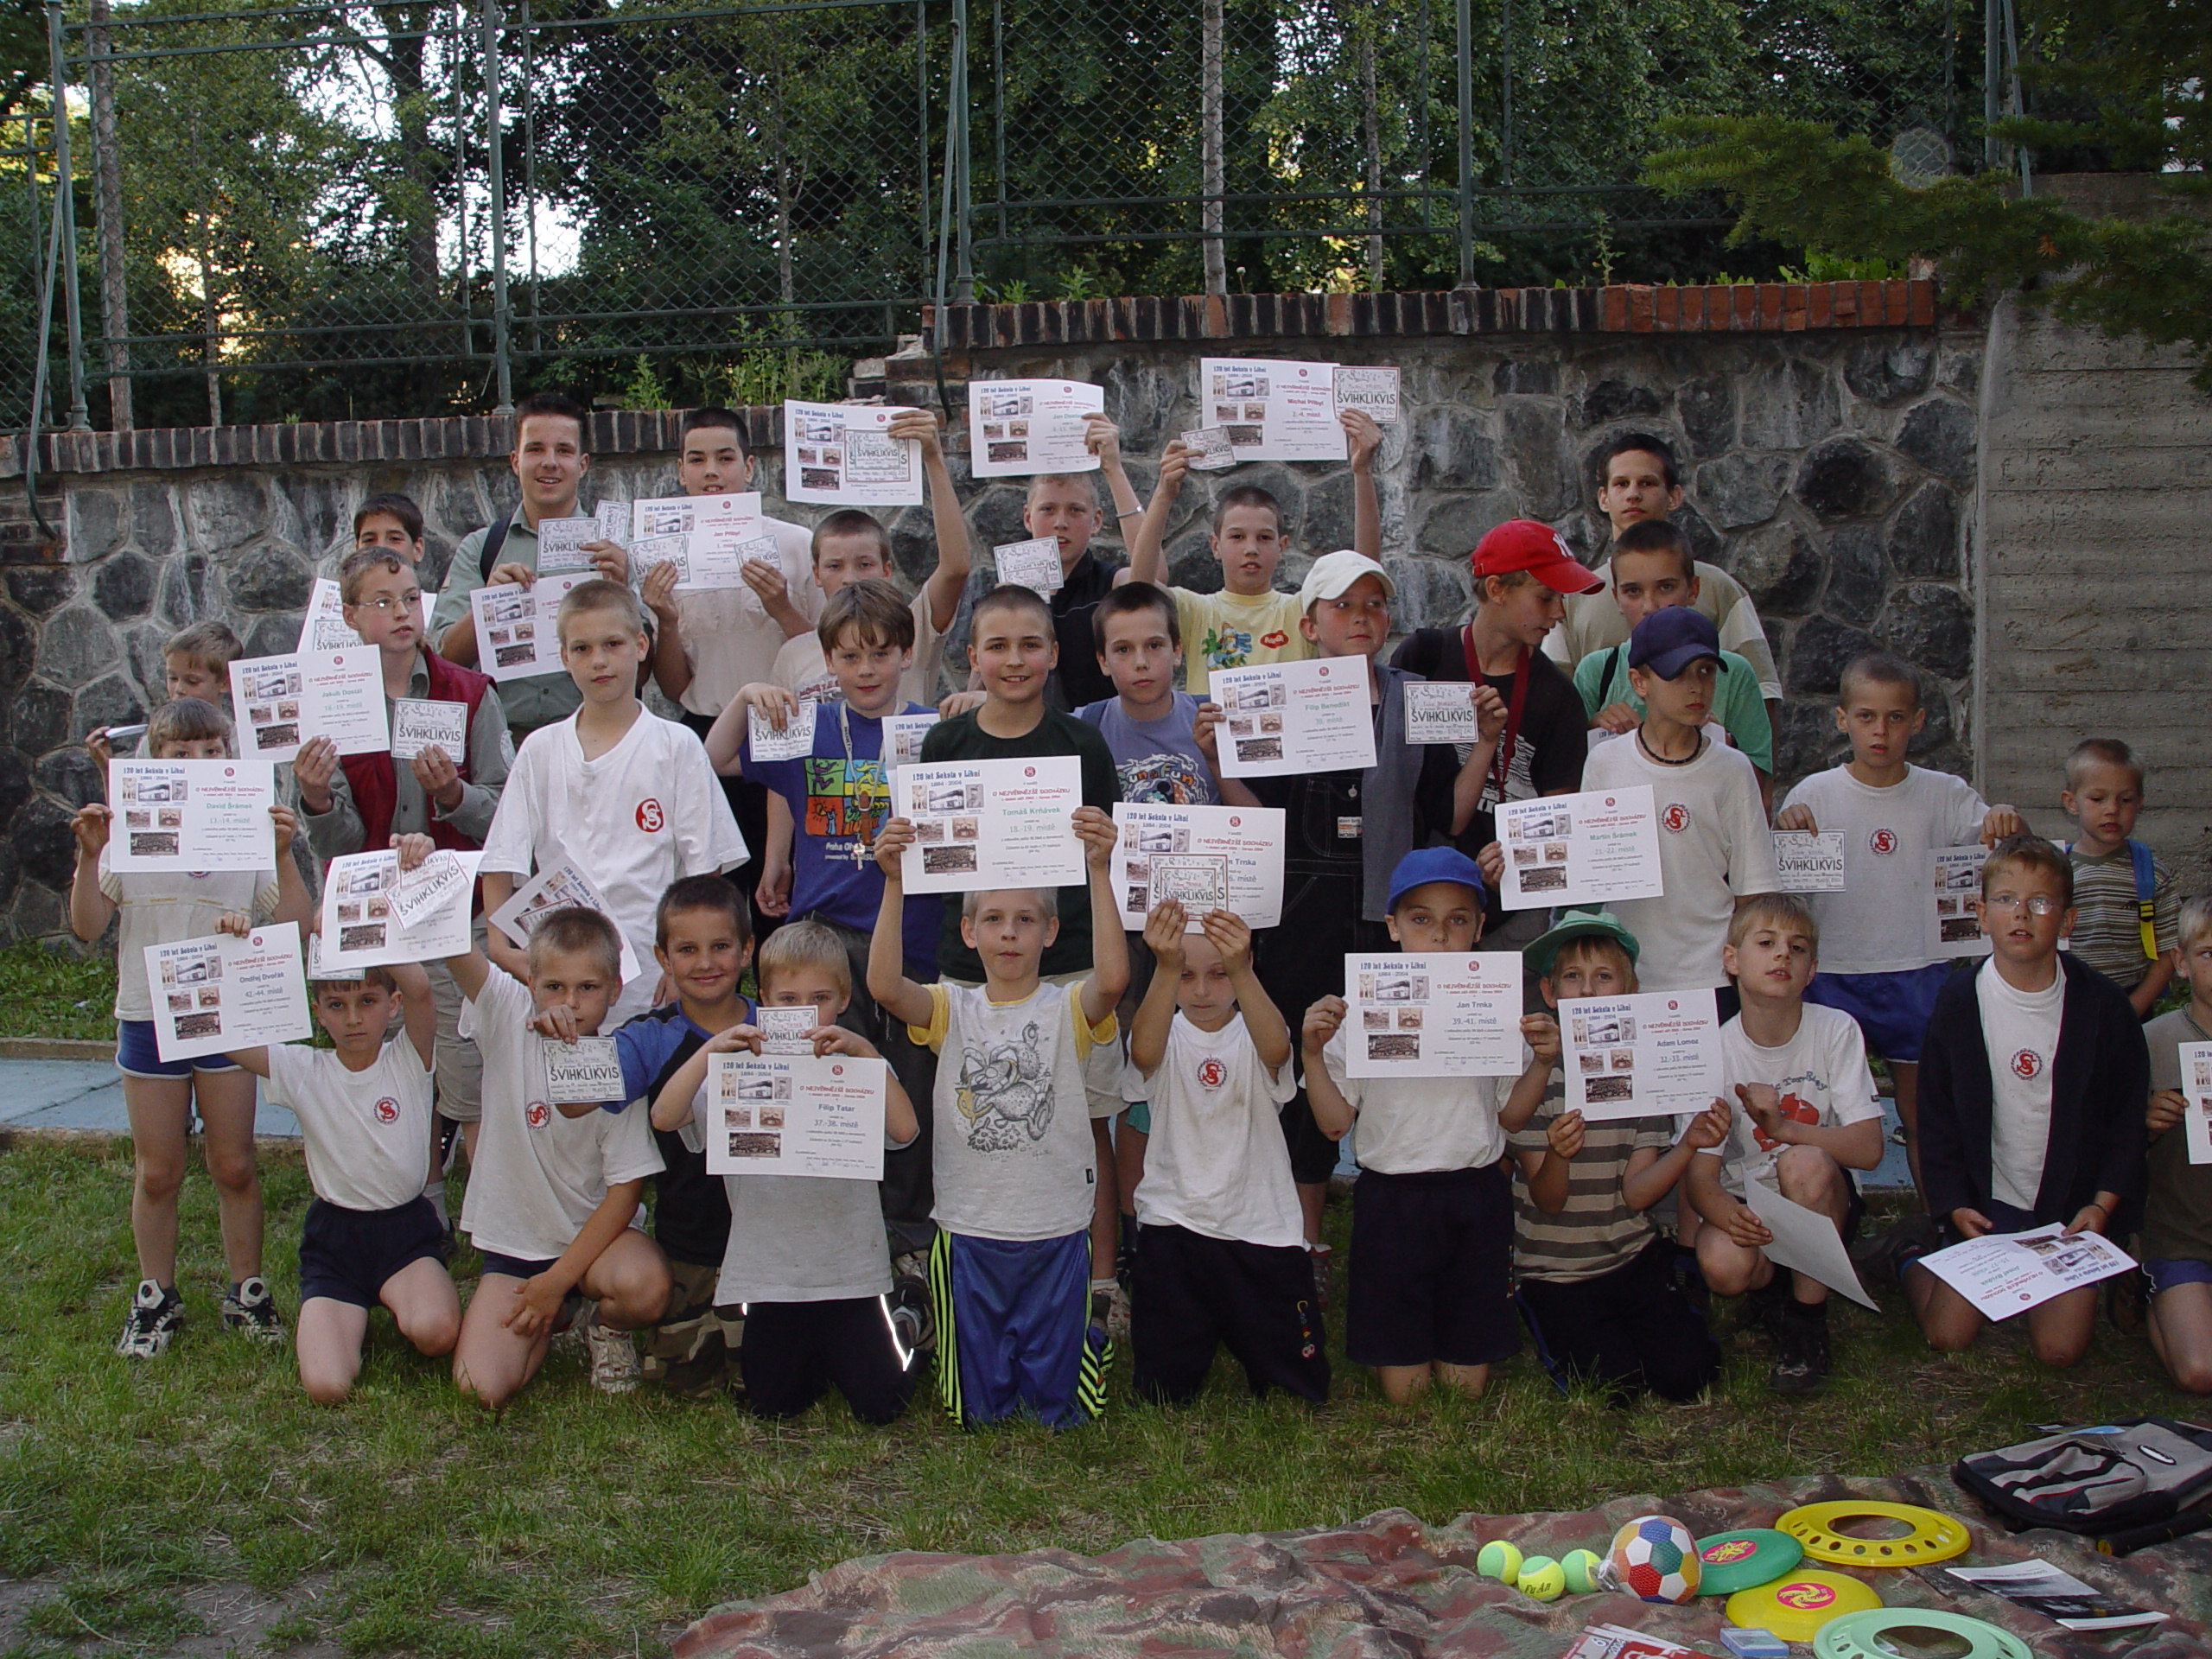
\includegraphics[width=0.9\textwidth]{img/37_vitezove_dochazka.JPG}
  \caption*{Vítězové soutěže O~Nejvěrnější docházku 2003/2004 z~řad mladších
  žáků, starších žáků a dorostenců, foto: archiv T.~J. Sokol Libeň}
\end{figure*}

V~následující tabulce uvádíme nejpilnější cvičence od roku 1995:

\renewcommand*{\arraystretch}{1.1}
\begin{longtable}[]{%
  >{\raggedright\arraybackslash}p{4em}%
  >{\raggedright\arraybackslash}p{1.4em}%
  >{\raggedright\arraybackslash}p{6em}%
  >{\raggedright\arraybackslash}p{6em}%
  >{\raggedright\arraybackslash}p{6em}}

\textbf{Cvičební rok} & \textbf{Max. hod.} & \textbf{Nejpilnější mladší žák} & \textbf{Nejpilnější starší žák} & \textbf{Nejpilnější dorostenec, cvičitel} \\
\hline \endhead
1995/1996 & 75 & Jakub Marianovský \(69\times\) & Jan Vorel \(69\times\) & Jiří Novák \(75\times\) \\
1996/1997 & 72 & Jan Bastin \(68\times\) & Jan Vorel \(72\times\) & ? \\
1997/1998 & 73 & Jáchym Kaplan, Martin Chlumský \(68\times\) & Jan Vorel \(71\times\) & Tomáš Novák \(73\times\) \\
1998/1999 & 77 & Tomáš Pajma \(68\times\) & Ondřej Antoš \(76\times\) & Jiří Novák \(77\times\) \\
1999/2000 & 78 & Jakub Mastík, Tomáš Pajma \(68\times\) & Jan Vorel \(78\times\) & Tomáš Seifert \(77\times\) \\
2000/2001 & 73 & Jan Přibyl \(63\times\) & Jakub Kudroň \(72\times\) & Martin Chlumský \(72\times\) \\
2001/2002 & 77 & Josef Drda \(69\times\) & Jakub Kudroň \(75\times\) & Martin Seifert \(77\times\) \\
2002/2003 & 74 & Štěpán Dvořák \(63\times\) & Jan Přibyl \(62\times\) & Jan Vorel \(74\times\) \\
2003/2004 & 77 & Jakub Novák \(69\times\) & Jan Přibyl \(76\times\) & Martin Seifert \(72\times\) \\
2004/2005 & 77 & Jan Trnka \(74\times\) & Jan Přibyl \(77\times\) & Jiří Novák \(76\times\) \\
2005/2006 & 80 & Jan Trnka 70 \(\times\) & Marek Šťovíček, Jan Salavec \(72\times\) & Jan Přibyl \(80\times\) \\
2006/2007 & 75 & Petr Jeřábek \(73\times\) & Josef Brůžek \(71\times\) & Jan Dostál \(74\times\) \\
2007/2008 & 76 & Petr Jeřábek \(72\times\) & Martin Jeřábek \(72\times\) & Jan Dostál \(75\times\) \\
2008/2009 & 78 & Richard Kloubský \(76\times\) & Martin Jeřábek \(68\times\) & Jan Dostál \(76\times\) \\
2009/2010 & 76 & Richard Kloubský \(74\times\) & Viktor Kubík \(63\times\) & Jan Přibyl \(76\times\) \\
2010/2011 & 75 & Richard Kloubský \(75\times\) & Petr Jeřábek \(68\times\) & Jan Přibyl \(75\times\) \\
2011/2012 & 78 & Jakub Málek \(75\times\) & Richard Kloubský \(78\times\) & Jan Přibyl \(78\times\) \\
2012/2013 & 77 & Kryštof Šubr \(69\times\) & Jakub Málek \(77\times\) & Jan Přibyl \(76\times\) \\
2013/2014 & 75 & Marek Novotný \(75\times\) & Adam Novotný, Richard Kloubský \(75\times\) & Jan Přibyl \(74\times\) \\
2014/2015 & 77 & Marek Novotný \(75\times\) & Richard Kloubský \(75\times\) & Vojtěch Mrkvička \(75\times\) \\
2015/2016 & 76 & Marek Novotný \(72\times\) & Viktor Šmejkal \(74\times\) & Richard Kloubský \(76\times\) \\
2016/2017 & 78 & Tomáš Novotný \(76\times\) & Marek Novotný \(76\times\) & Richard Kloubský \(78\times\) \\
2017/2018 & 74 & Tomáš Novotný \(71\times\) & Marek Novotný \(73\times\) & Richard Kloubský \(73\times\) \\
2018/2019 & 78 & Petr Ettel \(78\times\) & Tomáš Kléger \(77\times\) & Richard Kloubský, Jiří Novák \(78\times\) \\
2019/2020 & 61 & Tomáš Novotný \(61\times\) & Marek Matys \(58\times\) & Tomáš Kléger, Richard Kloubský \(61\times\) \\
2020/2021 & 28 & Michal Horák, Vojtěch Bőhm \(25\times\) & Tomáš Novotný \(26\times\) & Jiří Novák \(26\times\) \\
2021/2022 & 78 & Matyáš Sokol \(71\times\) & Petr Ettel \(74\times\) & Tomáš Kléger \(77\times\) \\
2022/2023 & 79 & Matyáš Sokol \(70\times\) & Jiří Smutný, Tomáš Novotný \(72\times\) & Tomáš Kléger \(78\times\) \\
2023/2024 & 77 & Ladislav Bednář \(73\times\) & Matyáš Sokol \(73\times\) & Jiří Novák \(77\times\) \\
\end{longtable}

\noindent
Také ihned započala éra letních a zimních soutěží pro žáky. Hned v~roce
1990/1991 to byly: Podzimní šplhavec, Jarní silák, Nářaďový pětiboj.
V~dalších letech to byly: pravidelně jarně-podzimní Letní disciplíny
(atletika a průpravné soutěže a závůdky) a přes zimu v~tělocvičně Zimní
soutěž. Postupem let to byly např.: O~nové kamarády, Silák roku (Petr
Špírek posiloval bez jediné vynechávky celý rok 1991/1992), Šplhavec,
Nářaďová pětka, O~kruha roku, Švihák, Minutový pěti- a sedmiboj, Míčový
pěti- a desetiboj, Zimní jedenáctiboj, Člunkový běh, Zimní trojboj,
Švihklikvis, Posilování, Šplh, Člunkový běh, různé Házení míče, Přeskoky
lavičky, Švihadla, Kliky, Předklony, Žebřiny, Výskoky na hrazdu,
Medicinbaly, Sprint, Shyby. Za všechny soutěže byli a jsou žáci
odměňováni drobnými věcnými cenami, sladkostmi a diplomy vyráběnými
cvičiteli.

\subsection{JVLS a PVLS}

Zdeněk Lauschmann přišel už na podzim 1990 s~myšlenkou společných
celojednotových výletů (aby nejezdily jen naše turistické oddíly
samostatně, ale abychom se navzájem -- členové jedné sokolské jednoty --
lépe poznali). A~tak vznikla tradice společných Podzimních a Jarních
Výletů Libeňského Sokola (PVLS a JVLS), která s~drobnou obměnou (od roku
1995 to Zdeněk rozšířil na jednoty celého pražského pětižupí) trvá
dodnes. Často bývala hostitelem mimopražská jednota, takže jsme své
přátelské vztahy rozšiřovali i za hranice Prahy. Určitě je třeba zmínit
milé přijetí v~Kutné Hoře či Nižboru.

\begin{figure*}[h!]
  \centering 
  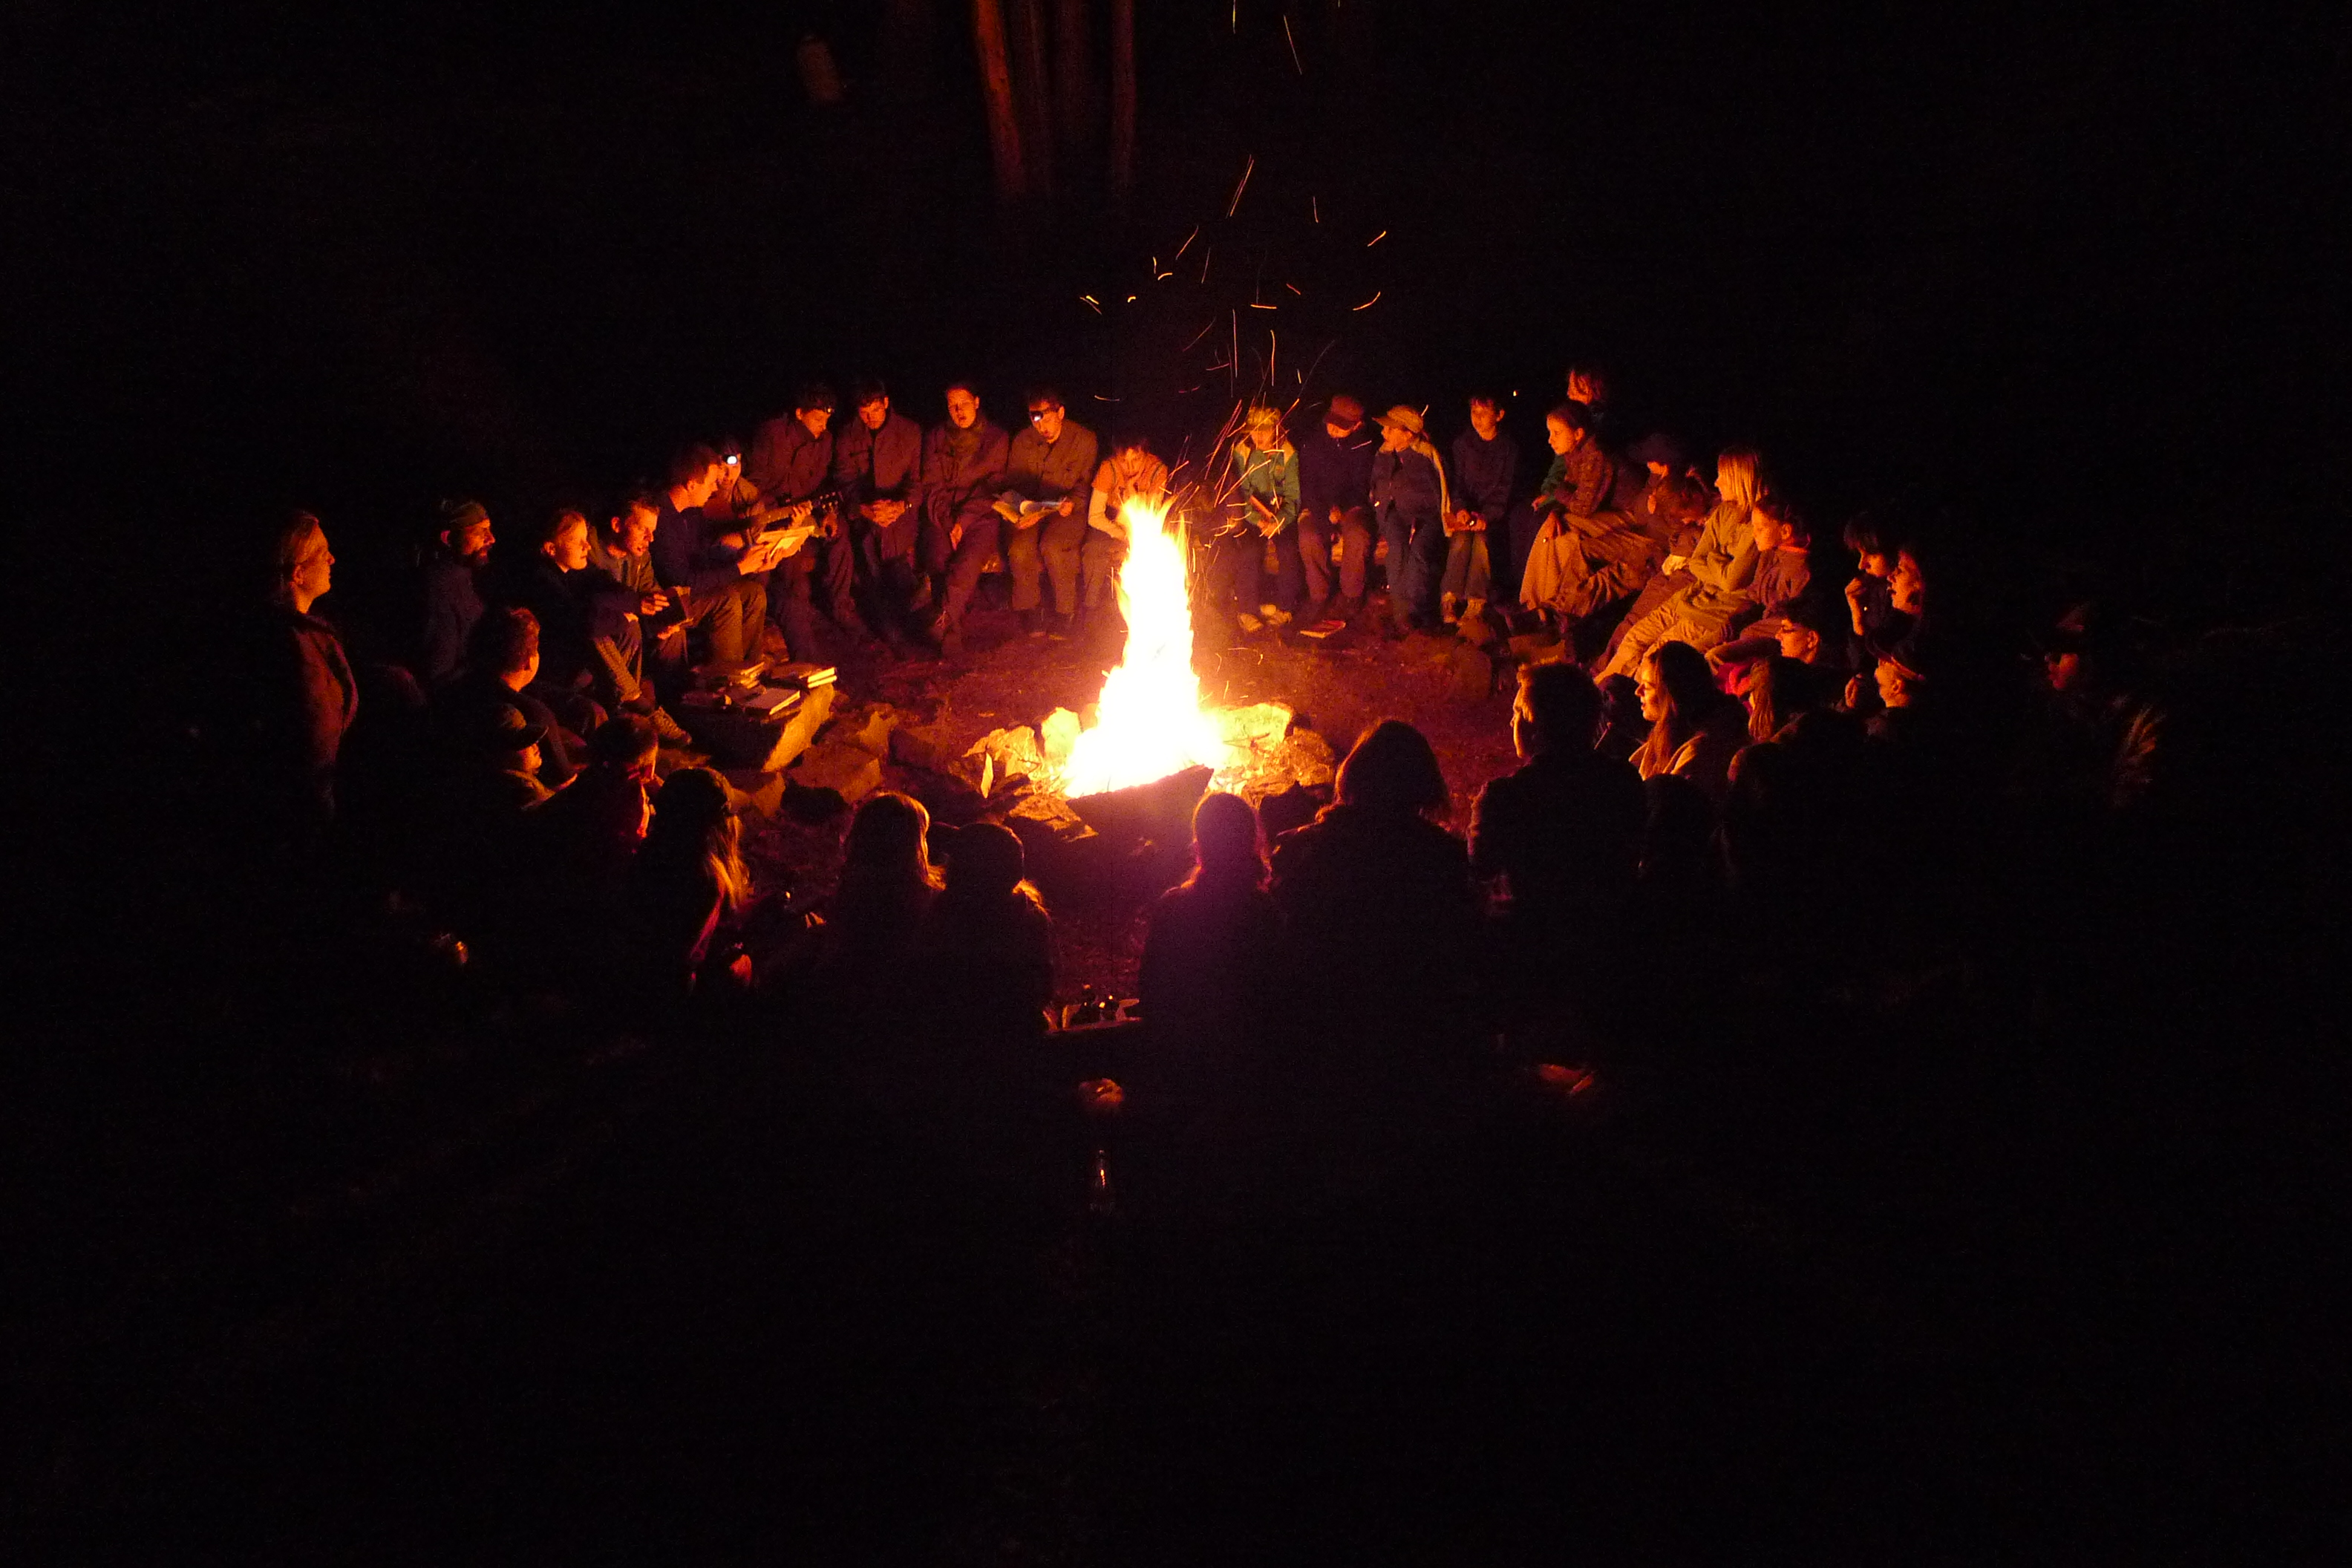
\includegraphics[width=0.9\textwidth]{img/38_jvls_taborak.JPG}
  \caption*{Večerní táborák JVLS 2011, Stará Dubá, foto: archiv JILMu}
\end{figure*}

A~zde jsou všechny naše uskutečněné výlety (rok, cíl + počet libeňských
účastníků -- mimochodem na oněch pětižupních srazech byla Libeň vždy
nejpočetněji zastoupenou jednotou a případně pořadatel pětižupního
srazu):

% TODO opakovat rok?
\renewcommand*{\arraystretch}{1.1}
\begin{longtable}[]{%
  >{\raggedright\arraybackslash}p{1cm}%
  >{\raggedright\arraybackslash}p{7.5cm}%
  >{\raggedright\arraybackslash}p{1.5cm}}
  \textbf{Rok} & \textbf{JVLS/PVLS -- místo (pořadatel)}  &  \textbf{Počet z~Libně} \\
 \hline \endhead
 1990  & 1. PVLS Hudlice, hájovna Na králi  &  79  \\
 1991  & 2. JVLS Nymburk a Chotuc  &  52  \\
 1991 &   3. PVLS Benešov a Kožlí  &  72  \\
 1992  & 4. JVLS Kutná Hora  &  92  \\
 1992 &   5. PVLS Čerčany a Lštění  &  88  \\
 1993  & 6. JVLS Pardubice a Kunětická Hora  &  92  \\
 1993 &   7. PVLS Skochovice a Vrané  &  80  \\
 1994  & 8. JVLS Nižbor  &  108  \\
 1994 &    9. PVLS Mšeno  &  90  \\
 1995  & 10. JVLS Skalka  &  73  \\
 1995 &   11. PVLS Klepec (1. sraz pětižupí, Zdeněk)  &  71  \\
 1996  & 12. JVLS Nižbor (poprvé ZZZ, Nižbor)  &  67  \\
 1996 &   13. PVLS Vinařická Hora (Zdeněk)  &  66  \\
 1997  &  14. JVLS Hudlice-Svatá  &  64  \\
 1997 &  15. PVLS Medník (Zdeněk)  &  43  \\
 1998 & 16. JVLS Malá Lečice (Zdeněk)  &  36  \\
 1998 &  17. PVLS Přerovská Hůra (Zdeněk)  &  94  \\
 1999  & 18. JVLS Nižbor (Nižbor)  &  52  \\
 1999 &   19. PVLS Blaník (Zdeněk)  &  83  \\
 2000  & 20. JVLS Hruboskalsko (není pětižupí)  &  48  \\
 2000 &  21. PVLS Nový Knín (Nový Knín)  &  49  \\
 2001  & 22. JVLS Lešetice (Libeň)  &  75  \\
 2001 &   23. PVLS Králův stolec (Dobříš)  &  67  \\
 2002 & 24. JVLS Radotínské údolí (Zlíchov)  &  44  \\
 2002 &  25. PVLS Mělník (Mělník)  &  65  \\
 2003  & 26. JVLS Zvířetice (Staré Město)  &  53  \\
 2003 &   27. PVLS Říčany (Říčany a Radošovice)  &  45  \\
 2004  & 28. JVLS Vrchlice, Cimburk (Libeň)  &  45  \\
 2004 &   29. PVLS Srbsko, lom Alkazar (Kobylisy)  &  30  \\
 2005  & 30. JVLS Újezd u~Zbečna (Zdeněk)  &  53  \\
 2005 &  31. PVLS Drahanské údolí (Troja)  &  51  \\
 2006  &  32. JVLS Velký Osek (Zdeněk)  &  49  \\
 2006 &  33. PVLS Zvolská Homole (Zdeněk)  &  36  \\
 2007  & 34. JVLS Poděbrady (Staré Město)  &  59  \\
 2007 &   35. PVLS Probošťská jezera (Kobyl., St. Město)  &  57  \\
 2008  &   36. JVLS Cholupice (Zdeněk)  &  46  \\
 2008 &  37. PVLS Lány (Zdeněk)  &  55  \\
 2009  & 38. JVLS Čelákovice (Zdeněk)  &  48  \\
 2009 &   39. PVLS Levý Hradec (Zdeněk)  &  57  \\
 2010  & 40. JVLS Radotínské údolí (Zdeněk)  &  40  \\
 2010 &   41. PVLS Strž u~Staré Huti (Dobříš)  &  37  \\
 2011  & 42. JVLS Stará Dubá (Libeň)  &  67  \\
 2011 &  43. PVLS Sadská, přesyp u~Píst (Kob., St. Město)  &  40  \\
 2012  & 44. JVLS Říčany, údolí Rokytky (Říčany)  &  63  \\
 2012 &  45. PVLS Mokropsy (Zdeněk)  &  90  \\
 2013  & 46. JVLS Malá Lečice (Zdeněk)  &  51  \\
 2013 &   47. PVLS Příbram -- Březové Hory (Břez. Hory)  &  64  \\
 2014  & 48. JVLS Vlčí rokle, Kam. Přívoz (Libeň)  &  71  \\
 2014 &  49. PVLS Kojetice, Lobkovice (Kobylisy)  &  48  \\
 2015  & 50. JVLS Károvský potok (Zdeněk)  &  65  \\
 2015 &   51. PVLS Klínec (Zdeněk)  &  42  \\
 2016  & 52. JVLS Králova stolice (Zdeněk)  &  66  \\
 2016 &   53. PVLS Tiché údolí (Kobylisy, Staré Město)  &  69  \\
 2017  & 54. JVLS Lučice (Libeň)  &  58  \\
 2017 &   55. PVLS Libčice (Libeň)  &  55  \\
 2018  & 56. JVLS Radotínské údolí (Zdeněk)  &  67  \\
 2018 &  57. PVLS Dubeč (Zdeněk)  &  84  \\
 2019  & 58. JVLS Závist (Libeň)  &  61  \\
 2019 &   59. PVLS Strž u~Staré Huti (Zdeněk)  &  76  \\
 2020  & covid -- zrušeno  &  \\
 2020 &   60. PVLS Dalejský potok (Zdeněk)  &  53  \\
 2021  & covid -- zrušeno  &  \\
 2021 &   61. PVLS Šárka (Zdeněk)  &  113  \\
 2022  &  62. JVLS Škvorec, Na plachtě (Libeň)  &  64  \\
 2022 &  63. PVLS Hloubětín, Kejřův mlýn (Zdeněk)  &  88  \\
 2023  & 64. JVLS lom Alkazar (Libeň, St.Město)  &  68  \\
 2023 &   65. PVLS Stará Dubá (Zlíchov)  &  83  \\
 2024  & 66. JVLS Kojetice, Lobkovice (Libeň)  &  89  \\
 2024 &   67. PVLS Červená Hlína (Zlíchov)  &  \\
\end{longtable}

Součástí JVLS je od roku 1996 i župní Zálesácký závod zdatnosti (ZZZ),
ze kterého se od roku 2001 postupuje na finále ČOS. Blíže o~něm v~článku
o~JILMu.

\begin{figure*}[h!]
  \centering 
  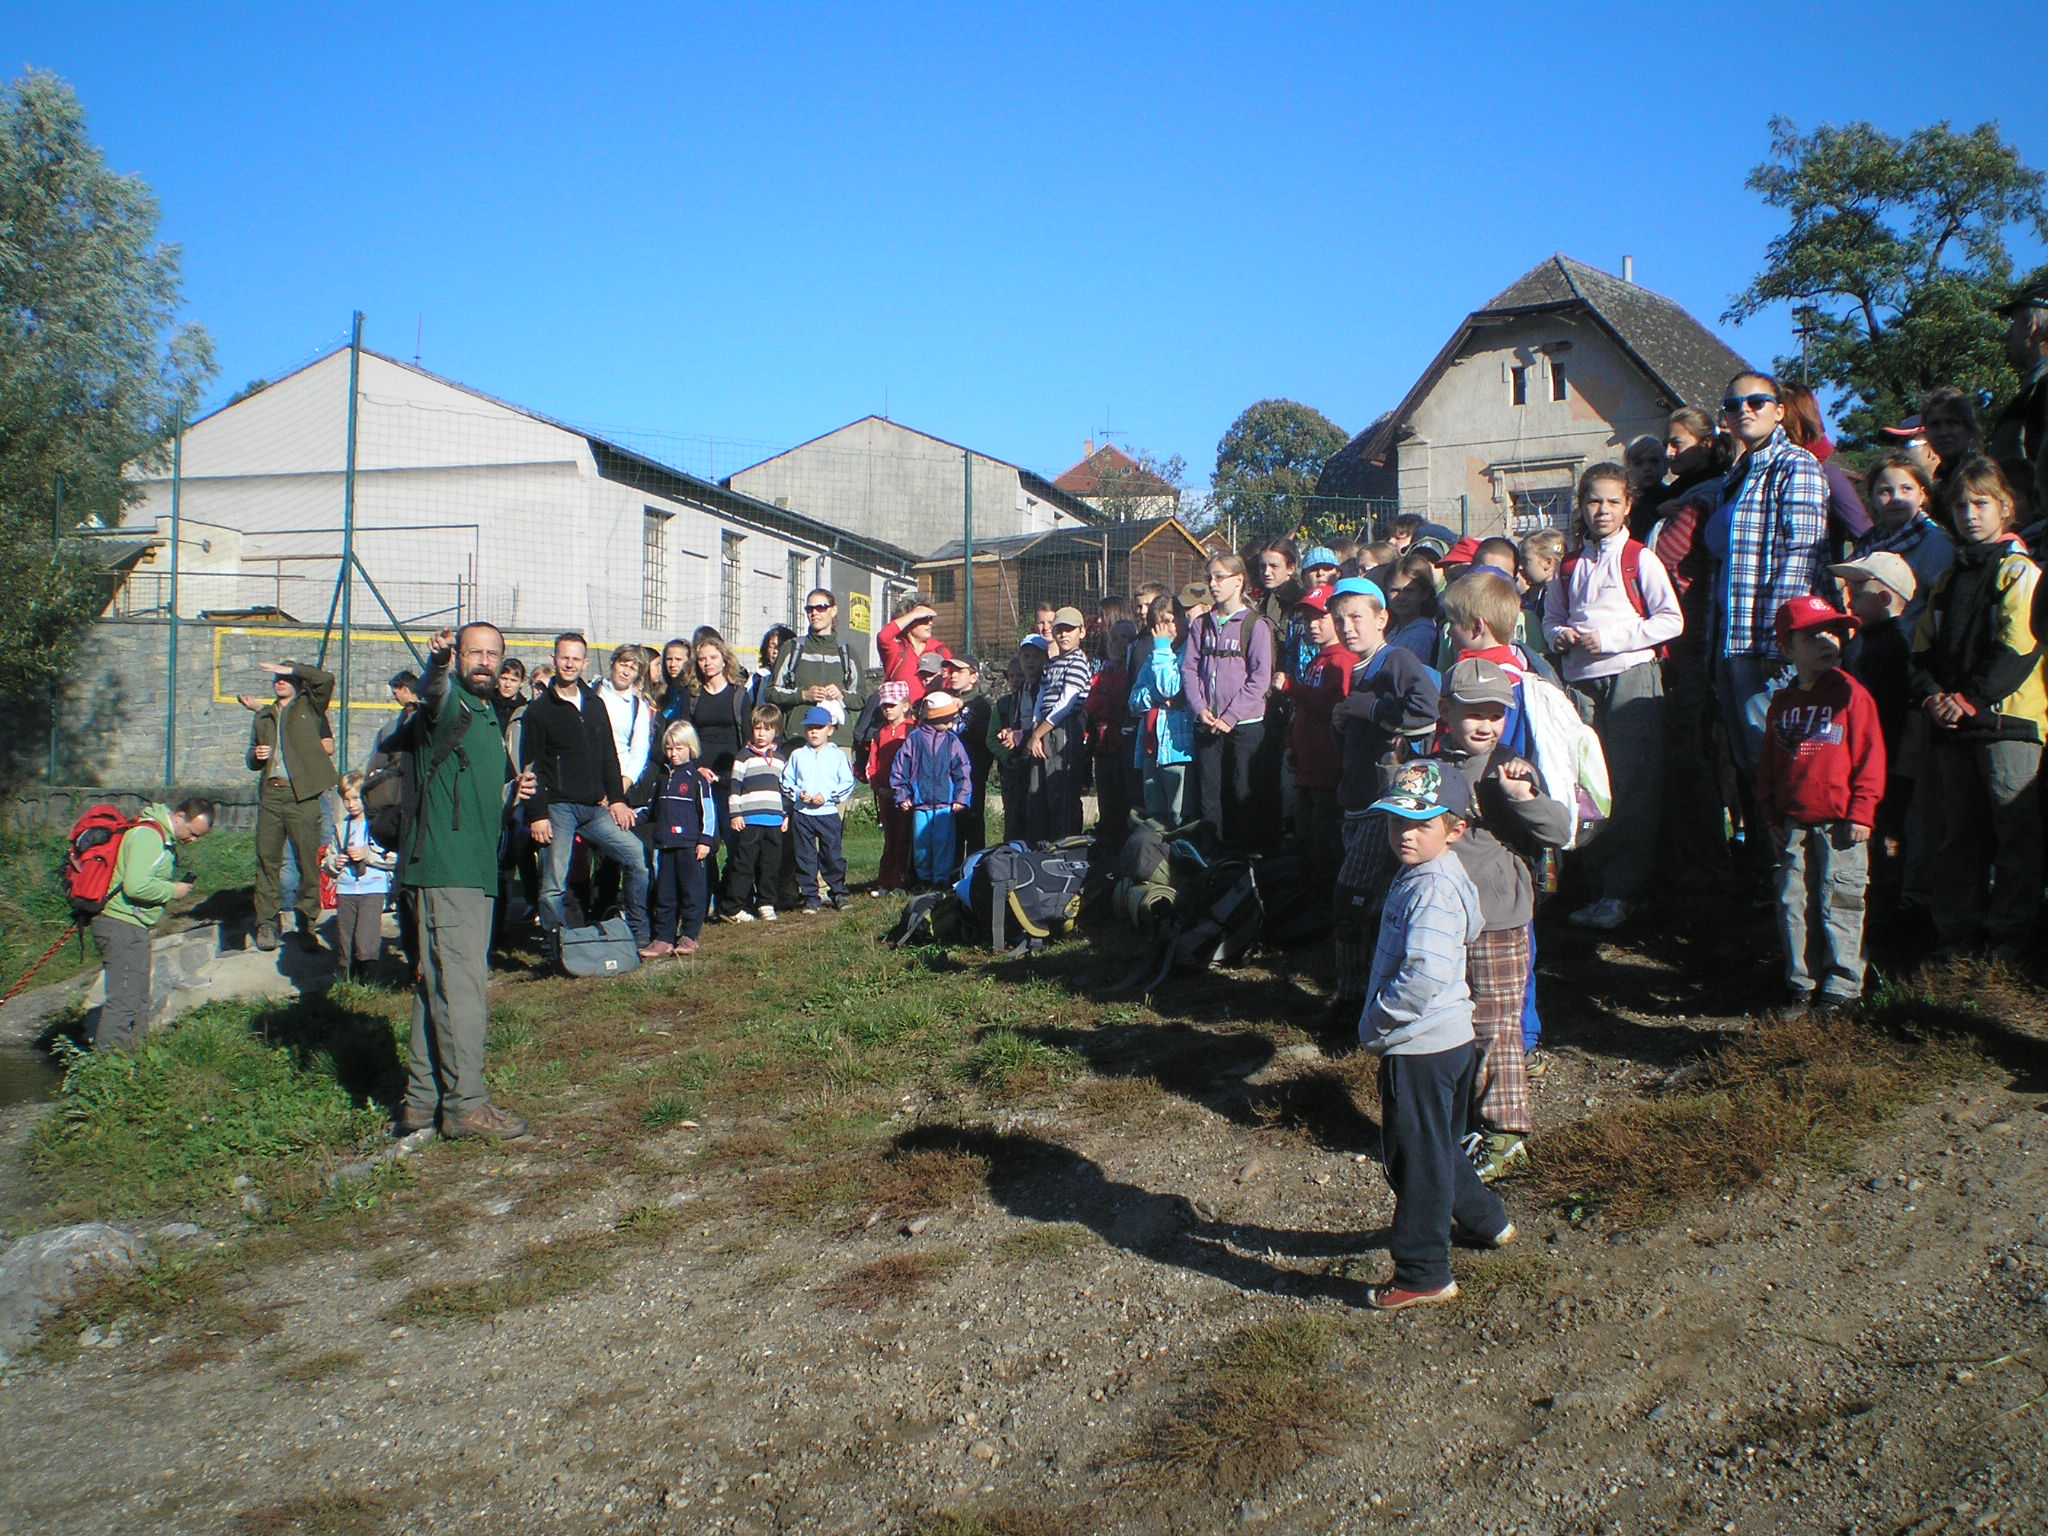
\includegraphics[width=0.9\textwidth]{img/39_pvls.JPG}
  \caption*{Podzimní Výlet Libeňského Sokola (a sraz v~přírodě pražského
  třížupí) 2012, Mokropsy, foto: archiv J. Přecha}
\end{figure*}

V~roce 1991 je také Loganem (br. Jiří Herzáň z~Třebíče) založena soutěž
Sokolský den v~přírodě. Soutěžilo se v~Zimním, Jarním, Letním a
Podzimním dni v~přírodě -- do každého se jednotě započítávají dny
prožité alespoň šestičlennou skupinou na vycházkách, výletech, výpravách
a táborech v~přírodě. Libeň se této soutěže účastnila od počátku, a i
díky pestré činnosti našich turistických oddílů (JILM, Káňata, Studánka,
Věrná garda a po určitou dobu i Pampelišky a letní tábory sportovní
gymnastiky) a pořádanými JVLS a PVLS si vždy vedla výtečně. Soutěž po
smrti zakladatele soutěže br. Herzána následně vedl br. Petr Mikysek
z~Mělníka a po jeho smrti a také pro úbytek účastnících se (reportujících)
jednot soutěž zanikla.

{\sloppy Zde je přehled celoročních výsledků (ty vzniknou po sečtení příslušných 4~dnů v~daném roce); náš součet činil vždy okolo 200 skupinodnů: \par}

%TODO odsadit jako tabulku - takhle?
\renewcommand{\arraystretch}{1}
\begin{longtable}{l p{10.2cm}}
1991 & 2. místo mezi 151 jednotami \\
1992 & 2. místo mezi 152 jednotami \\
1993 & 2. místo \\
1994 & 1. místo \\
1995 & 3. místo \\
1996 & 2. místo mezi 142 jednotami \\
1997 & 2. místo mezi 121 jednotami \\
1998 & 1. místo \\
1999 & 1. místo mezi 120 jednotami \\
2000 & 2. místo \\
2001 & 1. místo \\
2002 & 2. místo \\
2003 & 2. místo mezi 88 jednotami \\
2004 & 1. místo \\
2005 & 1. místo \\
2006 & 2. místo mezi 82 jednotami \\
2007 & 2. místo mezi 79 jednotami \\
2008 & 2. místo mezi 88 jednotami \\
2009 & 2. místo mezi 81 jednotami \\
2010 & 3. místo mezi 84 jednotami \\
2011 & 2. místo mezi 80 jednotami \\
2012 & 2. místo mezi 77 jednotami \\
2013 & 1. místo mezi 79 jednotami \\
2014 & 1. místo mezi 67 jednotami \\
2015 & 1. místo mezi 65 jednotami \\
2016 & 1. místo mezi 62 jednotami \\
2017 & 1. místo mezi 62 jednotami \\
2018 & počty dní odeslány, výsledky nejsou známy (\pozned{data od dědiců P.~Mikyska se komisi obytu v~přírodě nepodařilo získat, a tedy soutěž vyhodnotit, pozn. ed.}) \\
\end{longtable}

\subsection{Brigády}

Od počátku se konaly také brigády, ta asi první byla již na podzim 1990.
Zpočátku se vyklízely a uklízely jednotlivé místnosti, myla okna, praly
závěsy, postupně se začalo poklízet i okolí sokolovny. JILM a žáci si
vzali na starost zcela zpustlou jižní zahradu sokolovny a postupně se
z~džungle stala travnatá plocha, na níž si sami žáci a cvičitelé na jaře
1995 během 310 brigádnických hodin 41 lidiček vybudovali rozběžiště a
doskočiště pro skok daleký. Nejvíce hodin tenkrát odpracovali: Jirkan,
Mišina, Petra Šubrtová, Vláďa, Pavel, Vítek a Doník. JILM a žáci pak
dodnes tuto zahradu udržují (sekání trávy, čištění tarasu, sbírání
odpadků, zametání dlažby za sokolovnou; \pozned{toto byla realita roku
2004, v~roce 2013 bylo doskočiště i celá jižní zahrada zrekonstruovány
s~novou tartanovou dráhou a využívá ji také mateřská škola Nautis (dříve
APLA), která je u~nás v~nájmu, a o~sokolovnu i její okolí pečují
společně cvičitelé a členové napříč oddíly, pozn. ed.}). Pravidelné
jarní a podzimní brigády jsou součástí našeho programu do dnešních dní a
daří se nám tak udržovat vybavení v~provozuschopném stavu, dvakrát do
roka sokolovnu pořádně uklidit a zbavit nepořádku a v~neposlední řadě se
skoro pokaždé podaří i něco nového vytvořit. Namátkou lze jmenovat novou
vinylovou podlahu ve sborovně, opravu větracích šachet katakomb na
dvoře, které se začaly hroutit, nové dřevěné patro ve staré kotelně, na
kterém byla zbudována dílna i s~úložnými prostory, držáky gymballů
v~nářaďovně Srncova sálu a ve Strnadově sále, vykopání pařezů po
pokácených pajasanech a akátech, natření všech železných konstrukcí
v~sále kovářskou černí, zbourání plechových garáží na dvoře a stovky
dalších drobných prací a splněných úkolů.

Během roku 1992 se díky br. Kubištovi podařilo dokončit plynofikaci
kotelny (předtím se topilo koksem) a tím i ušetřit peníze za mzdy
kotelníků. Další výměna kotlů proběhla asi po deseti letech a v~roce
2011 byla nová kotelna vystavěna v~dřívější dílně údržbáře. A~ta nám
slouží dodnes.

\begin{figure*}[h!]
  \centering 
  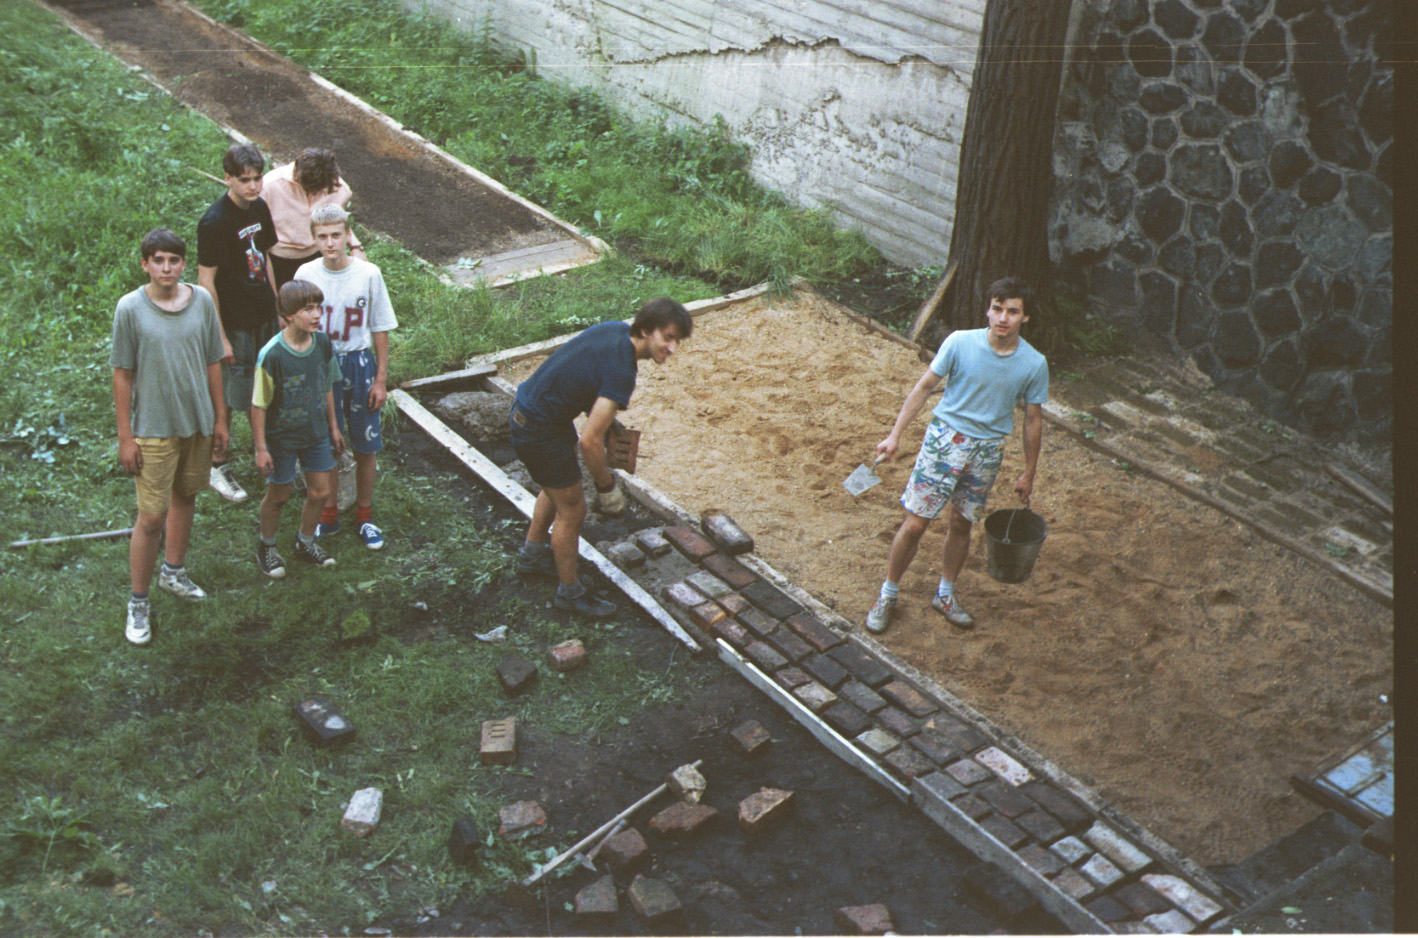
\includegraphics[width=0.9\textwidth]{img/40_doskociste.jpg}
  \caption*{Vylepšování doskočiště na jižní zahradě sokolovny (1995), foto: archiv T.~J. Sokol Libeň}
\end{figure*}


\subsection{Mikuláš}

Další tradicí, kterou nepřerušily ani zmatky a nejistota okolo roku
1989, je Mikuláš. Chodil do sokolovny i v~70. a 80. letech a nepřestal
dodnes. Vždy přijde důstojný Mikuláš, roztomilí andělé a většinou celá
kupa "zlých" čertů. Děti se předvedou na nářadí, při čertovské
rozcvičce anebo, jako v~posledních letech, při různých básničkách ve
svíčkami osvětleném sále. Konec je však vždycky stejný -- rozdávání
balíčků z~rukou andělů. Hodných dětí se takto každoročně sejde 100--200.
Tradici Miluláše nepřerušil ani covid. V~roce 2020 a 2021 se mikulášská
nadílka konala na zahradě sokolovny pro postupně přicházející děti.

\begin{figure*}[h!]
  \centering 
  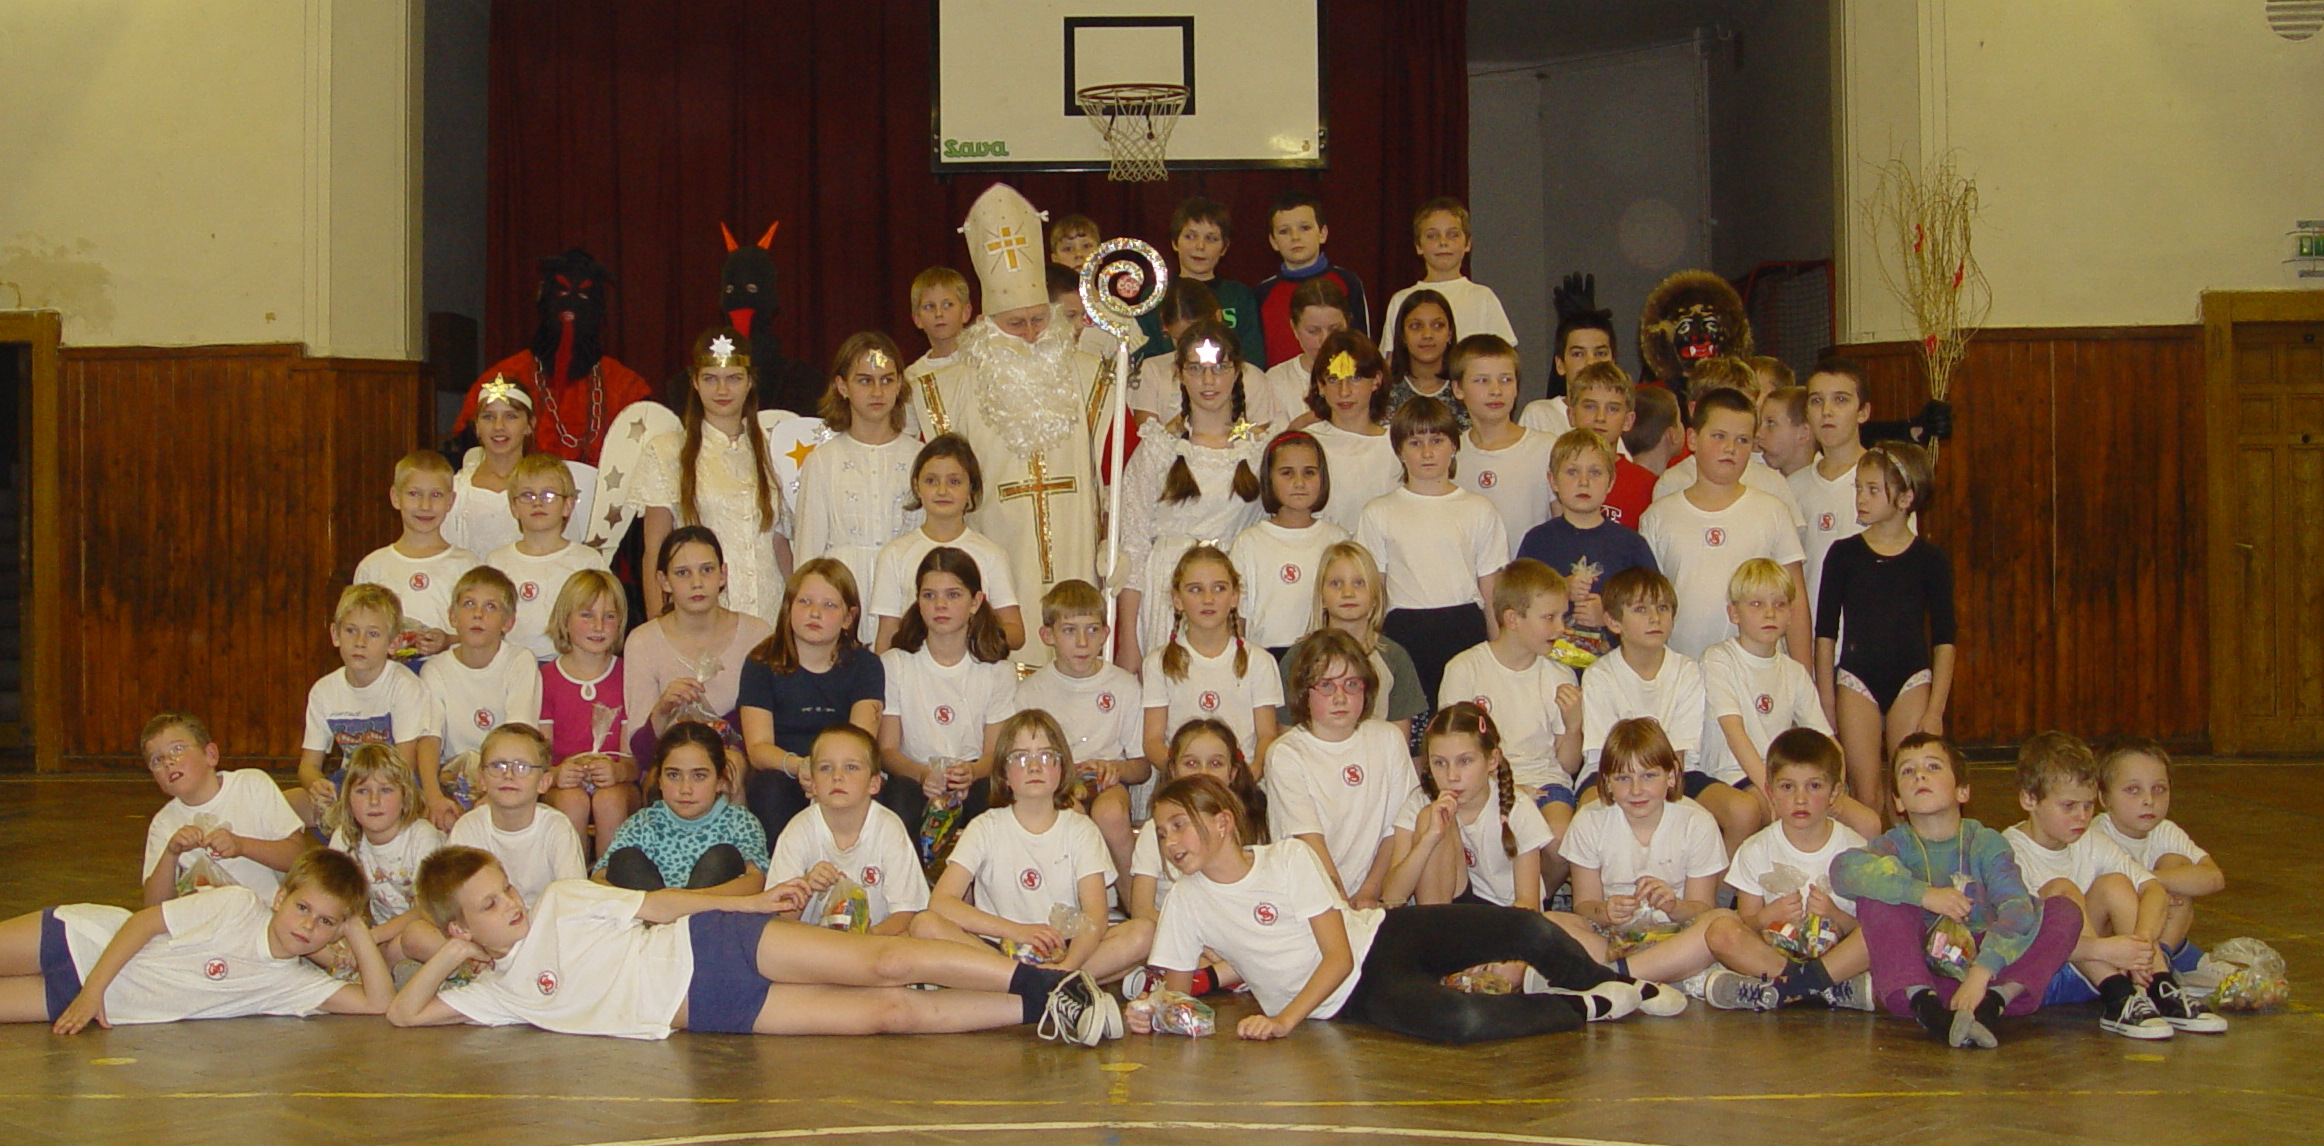
\includegraphics[width=0.9\textwidth]{img/41_mikulas.JPG}
  \caption*{Mikuláš, mladší žactvo (2003), foto: archiv T.~J. Sokol Libeň}
\end{figure*}

\subsection{Závody sokolské všestrannosti}

Na jaře roku 1992 jsme obnovili naši účast na gymnastických přeborech
(jedná se o~přebory ve sportovní gymnastice neregistrovaných závodníků)
a také vyslali 4~dorostence na pomahatelský kurz. Další přebory
v~gymnastice se konaly přímo v~naší sokolovně na jaře 1993. Mladší žáci
vybojovali ve šplhu 1., 2. i 3. místo, starší zase zvítězili
v~družstvech. Od té doby se účastníme těchto přeborů každoročně. Každý rok
se tak téměř 3 měsíce věnujeme 15--30 vybraným hochům a učíme je zvládat
gymnastické sestavy. Kluci sice většinou v~celopražském měřítku nemají
na nejlepší, ale občas se nějaký úspěch najde. Skoro vždy dominujeme ve
šplhu jako doplňkové disciplíně a v~posledních letech se i díky
(bohužel) menšímu počtu soupeřů dostáváme do dalších kol. A~tak se na
prestižní závod Praha -- Brno -- Bratislava probojovali v~roce 2000 J.
Michálek a 2002 J. Vorel a J. Kudroň.

V~polovině 90. let došlo k~částečné reorganizaci soutěže -- přejmenována
na Přebor všestrannosti -- má 4 disciplíny: atletika (sprint, skok
daleký, hod krikeťákem, dlouhý běh), gymnastika (přeskok, kruhy, hrazda,
akrobacie, bradla), šplh a plavání. První dva mladší žáci v~župě vytvoří
spolu s~nejlepšími žákyněmi družstvo a soutěží pak v~celostátním finále
ČOS, u~starších postupují první dva do celostátního finále ČOS
jednotlivců. Za župu Barákovu nás tak v~roce 1999 v~Písku reprezentovali
mladší žáci J. Michálek a J. Kudroň a v~roce 2001 D. Khol, pak se závod
mladších přesunul do Plzně, kde v~roce 2003 závodili T. Marek, M.
Přibyl, V. Strieborný a E. Novák a v~roce 2004 J. Budil (7. místo), J.
Michalec, T. Marek a M. Přibyl. Starší mají finále vždy v~Praze --
v~roce 2001 se do něj probojoval J.~Vorel, v~roce 2003 J. Kudroň a v~roce
2004 O. Loudil, O. Michalec a J. Novák. V~tomto roce jsme měli
zastoupení i mezi dorostenci -- J. Kudroň a J. Vorel.

\begin{figure*}[h!]
  \centering 
  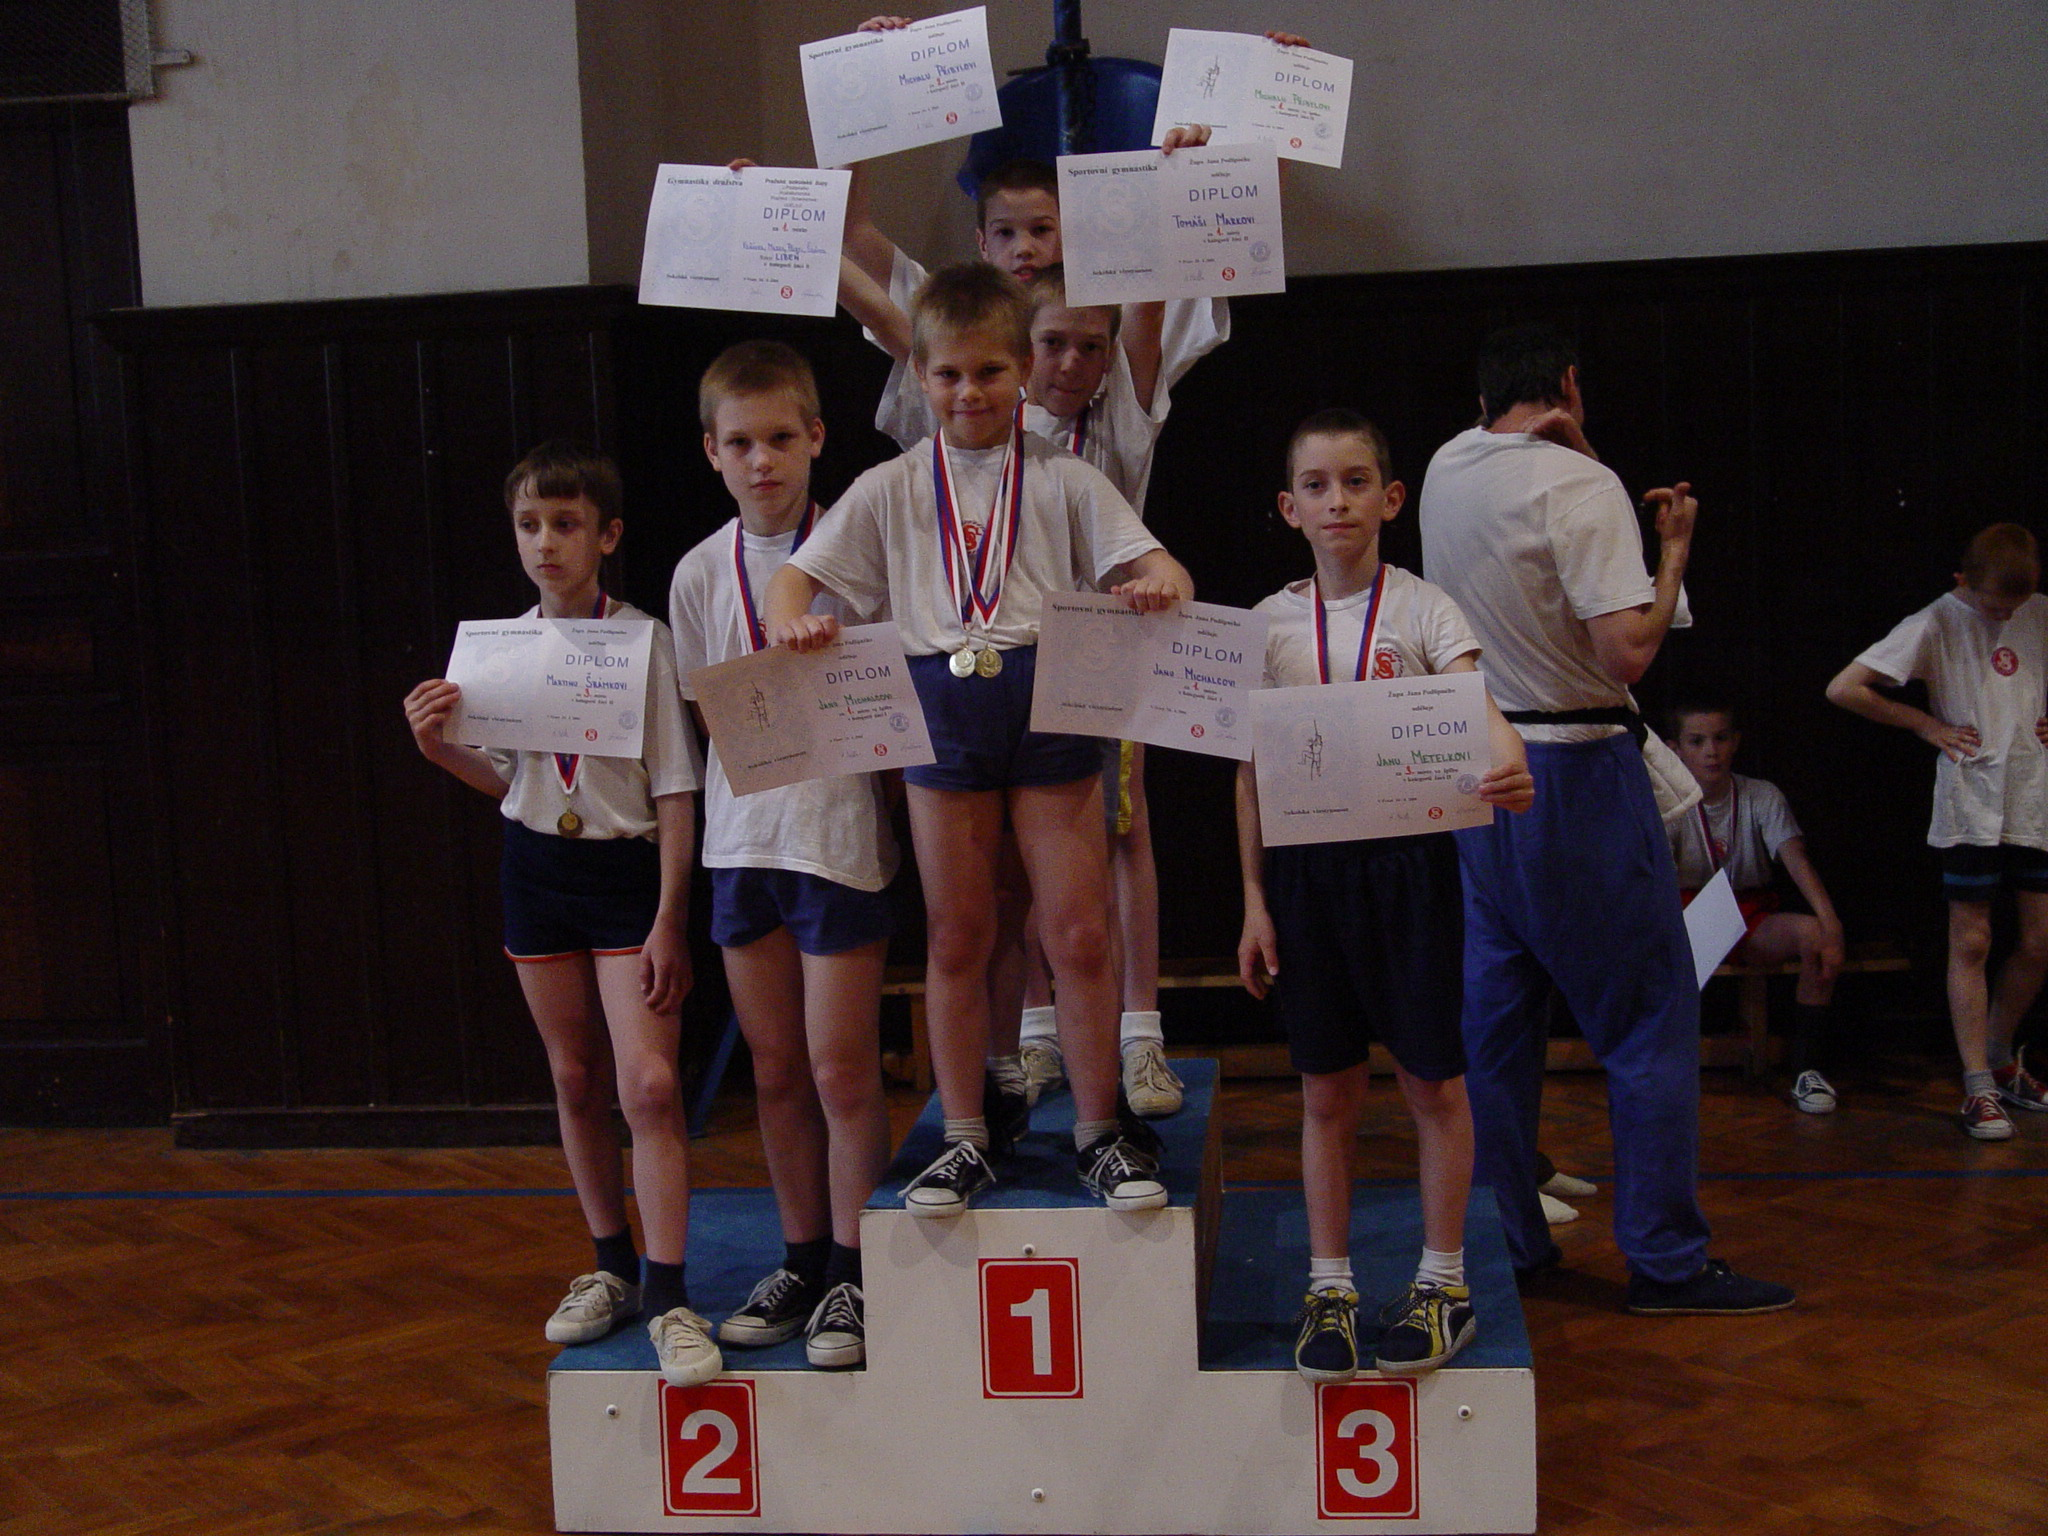
\includegraphics[width=0.9\textwidth]{img/42_vitezove_gumnastika.JPG}
  \caption*{Vítězné družstvo mladších žáků na závodech všestrannosti ve
  sportovní gymnastice 2004, Jan Michalec (uprostřed vpředu), Michal
  Přibyl (uprostřed vzadu) a Jan Metelka (vpravo) mají ještě individuální
  úspěchy ze závodu ve šplhu, foto: archiv T.~J. Sokol Libeň}
\end{figure*}

Povšimněte si, že mezi závodníky lze nalézt jména budoucích cvičitelů:
Pavel Voráč, Vít Jakoubek, Tomáš Seifert, Jan Vorel, Jakub Kudroň,
Michal Přibyl. Závody všestrannosti se konají stále. Nejprve je Přebor
župy a z~něj postupují nejlepší závodníci na přebor ČOS. Na finále
všestrannosti ČOS nechyběli naši závodníci od roku 2004 do roku 2024 ani
jednou. Výjimkou byly pouze dva covidové roky 2020 a 2021, kdy se závody
nekonaly.

Aby se zachoval závod o~přeborníka Prahy, byla časem (někdy okolo roku
2010) zavedena soutěž Praha Open, do které postupují nejlepší závodníci
tří pražských sokolských žup a dále závodníci ASPV (Asociace sportu pro
všechny). I~naši závodníci se tedy tohoto závodu pravidelně každoročně
účastní.

\subsection{Cvičení dorostenců a mužů v~90.
letech}

Od roku 1992 přibyla hodina pro dorost. Nejprve jsme poctivě střídali
volejbal a košíkovou, která se posléze stala jedinou náplní této hodiny.
V~listopadu 1992 jsme sehráli přátelské utkání v~košíkové s~dorostenci
z~Lysé -- bohužel jsme prohráli. Čtvrteční "cvičitelská" košíková je
pravidelnou součástí rozvrhu i v~roce 2024. Od podzimu 1992 bylo na
několik let obnoveno i cvičení starších mužů pod vedením starosty
Ladislava Mrklase. Mladší muže (nejraději si zahrají fotbálek) vedou až
do dnešních dnů Roman a Jan Kolář (\textit{až na to, že už nejsou
"mladší", pozn. ed.}).

\subsection{Dětský den}

Koncem května 1992 se koná první Dětský den -- na louce u~studánky je
připraveno 9 disciplín a na konci vystoupení skupiny historického šermu
Valdštejnové, kteří trénují v~naší sokolovně. Účast činí 46 dětí, které
dostávají při splnění úkolu žetony, které lze posléze vyměnit za
sladkosti.

Tím byla založena tradice Dětských dnů, která trvá dodnes. Počet soutěží
se postupně rozrůstal na 15, 17, 21 a od roku 2003 na 27. V~počátcích
přišel dvakrát i kouzelník, šermíři chodí dodnes (pouze jejich jméno je
jiné -- Streitax), od roku 1995 se přidalo sjíždění Rokytky na kánoích a
od roku 1997 se také přešlo od žetonů na lejstra, do nichž děti
dostávají barevná razítka (gotická písmena). Počet pořadatelů postupně
narůstal s~počtem soutěží a dnes jich je potřeba okolo 50 -- proto
dostávají šanci kromě cvičitelů i žáci a žákyně, turistické oddíly a
další pomocníci. Narostl i počet dětí, jak dokládá přiložená
tabulka. V~letech 2020 a 2021, kdy řádil covid, se konal Dětský den
individuálně s~obcházením mnoha stanovišť po Libni s~plněním úkolů a
luštěním kódu k~odemčení truhly s~pokladem v~sokolovně.

\renewcommand*{\arraystretch}{1.1}
\begin{longtable}[]{%
  >{\raggedright\arraybackslash}p{1cm}%
  >{\raggedright\arraybackslash}p{2cm}%
  >{\raggedright\arraybackslash}p{1cm}%
  >{\raggedright\arraybackslash}p{2cm}%
  >{\raggedright\arraybackslash}p{1cm}%
  >{\raggedright\arraybackslash}p{2cm}}
 \textbf{Rok} &  \textbf{Počet dětí} &  \textbf{Rok} &  \textbf{Počet dětí} &  \textbf{Rok} &  \textbf{Počet dětí} \\
 \hline \endhead
 1997 &  180 &  2007 &  225 &  2017 &  260 \\
 1998 &  129 &  2008 &  243 &  2018 &  155 \\
 1999 &  241 &  2009 &  150 &  2019 &  102 \\
 2000 &  183 &  2010 &  145 &  2020 &  covid \\
 2001 &  148 &  2011 &  220* &  2021 &  covid \\
 2002 &  183 &  2012 &  234* &  2022 &  240 \\
 2003 &  228 &  2013 &  104* &  2023 &  270 \\
 2004 &  131 &  2014 &  109* &  2024 &  160 \\
 2005 &  185 &  2015 &  200 & {} & {} \\
 2006 &  155 &  2016 &  150* & {} & {} \\
\end{longtable}
\vspace*{-1.2\baselineskip}
*v těchto deštivých letech se konal Dětský den v~sokolovně

\begin{figure*}[h!]
  \centering 
  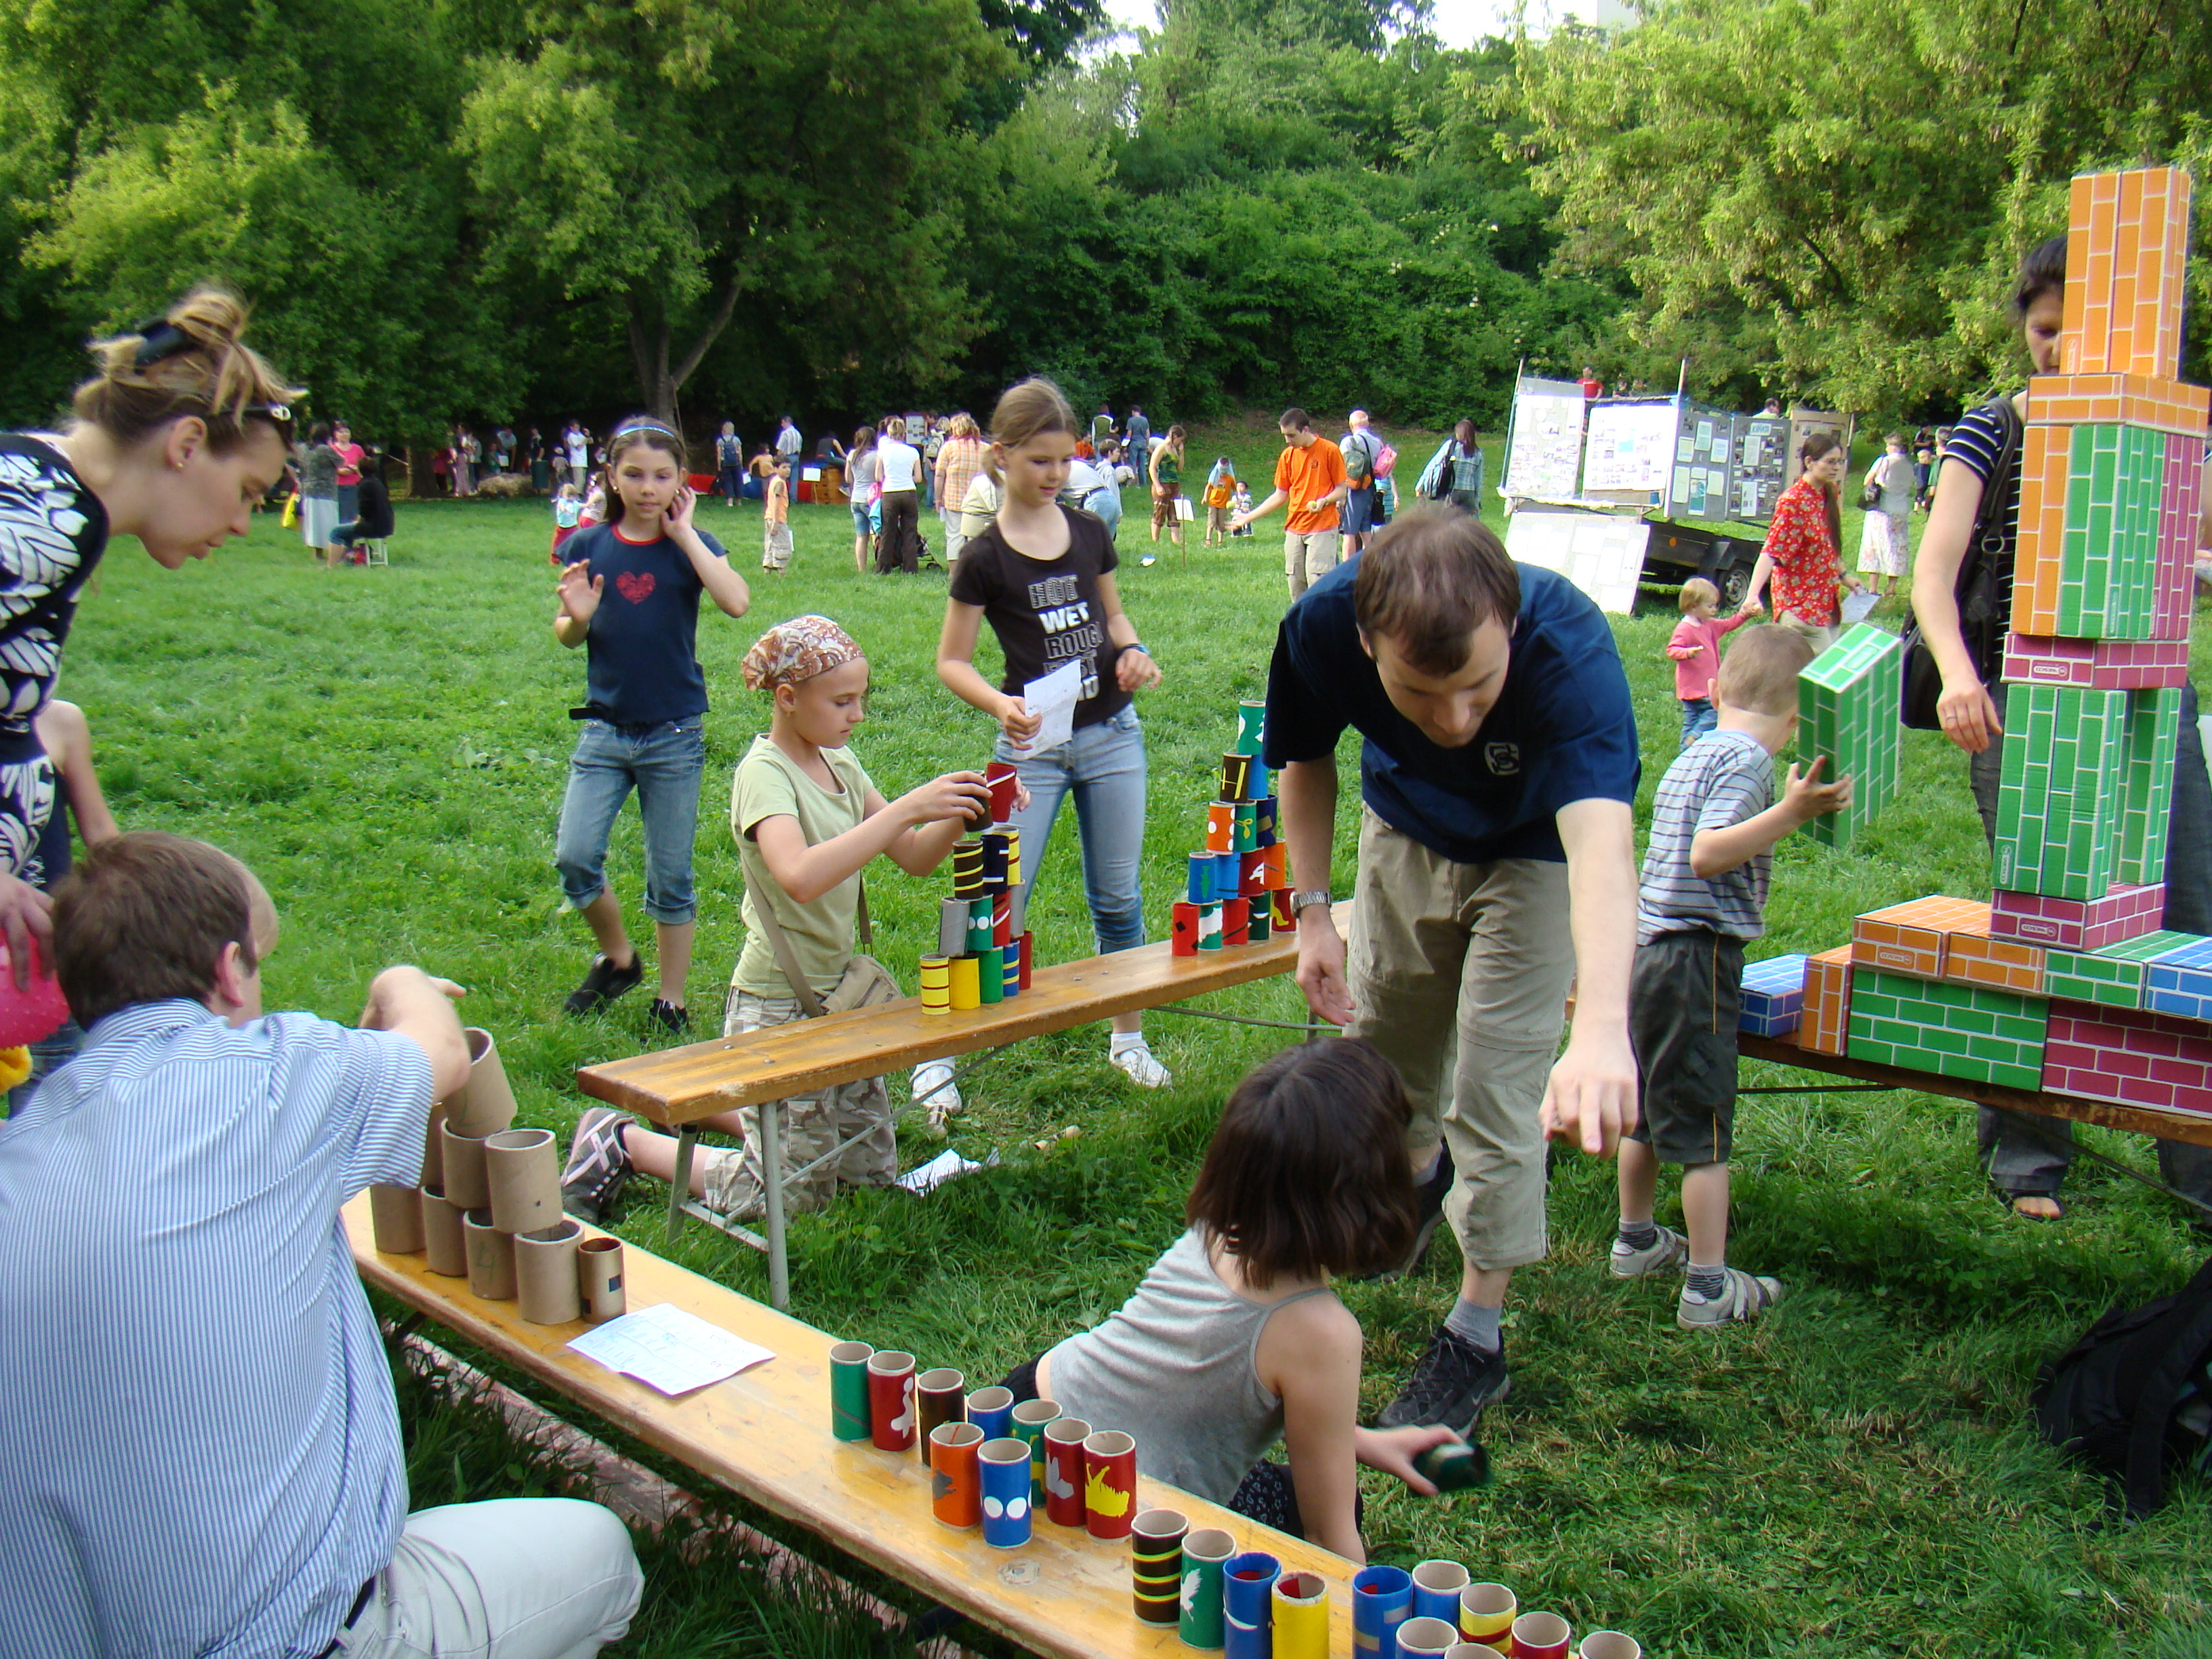
\includegraphics[width=0.9\textwidth]{img/43_detsky_den.JPG}
  \caption*{Dětský den 2008, louka u~studánky, foto: archiv J. Přecha}
\end{figure*}

\subsection{Sokolí boudy v~Malé Úpě}

Do navrácených Sokolích bud v~Krkonoších se vydává na akci Povánoce 1992
13~žáků a dorostenců s~2 rodiči a 2 cvičiteli. V~létě se pak na celý
týden vydává 8~dorostenců a cvičitelů na Ohři jako vodáci. Akce Povánoce
1993 se koná za účasti 25~osob. Na Sokolí boudy jezdil na zimní pobyty
také oddíl Studánka. Ovšem Sokolí boudy jsme nakonec v~roce 2001
prodali, protože jsme potřebovali peníze na opravu sokolovny.

\subsection{Tělocvičné akademie}

V~dubnu 1993 se koná první Tělocvičná akademie s~připravenými čísly. Už
v~říjnu 1991 však byla Veřejná cvičební hodina s~předvedením ukázek
cvičení. Postupem času se termín akademie přesunul na méně exponovaný
termín (na jaře se pilně nacvičuje na závody) a tím se stal přelom října
a listopadu. Oproti většině jiných jednot vystupují na akademii téměř
výhradně naši cvičenci -- od rodičů s~dětmi a předškolňat přes žactvo až
po Věrnou gardu a muže. Občas vystoupili šermíři, v~době působení oddílu
sportovní gymnastiky jsme obdivovali jejich umění, pouze výjimečně u~nás
vystupují hosté z~jiných jednot. Akademie trvá přibližně 2 hodiny a má
okolo 12--14 bodů programu. Počet cvičenců vždy vysoko přesahuje číslo
100, občas se blíží 200. Diváci obsazují cca 120 židlí postavených
v~třetině sálu a houfně také galerii -- bývá jich 200--300. V~počátcích se
o~průvodní slovo staral skvělým způsobem br. František Kodl, po jeho
úmrtí uváděli jednotlivá čísla cvičitelé, vedoucí Káňat Drb a Kačka a
v~poslední době se konferenciérství ujal náš cvičitel Martin Chlumský
zvaný Čedok (\pozned{současný starosta ČOS, pozn. ed.}). Za ta léta možná
uvízla ve Vaší paměti kromě běžných závůdků mladších žáků, ukázek
sletových skladeb a cvičení na nářadí tato čísla našich žáků a
dorostenců: Rej na lavičkách, Přeskoky, Pompony, Cvičení ve trojicích +
pochodový rej vedený údery tyče o~zem, skladba mladších žáků s~tyčemi
pro župní slet v~Brandýse, Aerobik cvičitelů, pohádka JILMu Kašpárek a
Pelerini, případně vystoupení JILMu se stavbou týpka, divadelní koláž
Cvičební rok, Country tance, Správní kluci atd. Zvláště pečlivě byly
připravovány akademie ke 110. a 115. výročí (1994 a 1999) a také v~roce
2000 k~90. výročí postavení sokolovny či roku 2002 na počest dokončení
obnovy fasády. Výroční akademie byly spojovány s~výstavou o~historii ve
Filipově síni (pečlivě připravované Věrnou gardou). Samozřejmostí byla
účast vzácných hostů mezi diváky (lidé z~vedení žup a ČOS, starostové
Prahy 8 atd.).

Postupně jsme začali naše akademie natáčet a DVD se záznamem
distribuovat mezi naše členy. V~dnešní době se jim už jen zašle odkaz na
náš YouTube kanál. Akademie samozřejmě i nadále probíhají každý rok
(většinou okolo 20.~listopadu, výjimku tvořil rok 2020, kdy se akademie
nekonala kvůli covidu, a roky 2021 a 2023, kdy byla přesunuta na jaro
z~důvodu covidu a následně kvůli rekonstrukci šaten). Diváků i cvičenců je
stále více, a tak se zvětšilo i hlediště v~sále, kde už je okolo 210
židlí (a ve třech výškových úrovních -- na zemi, na nízkém a na vyšším
pódiu tak, aby všichni diváci dobře viděli) a ještě jsou před diváky
lavičky pro dětské cvičence. Cvičenců bývá mezi 200 a 300 a diváků mezi
250 a 400. Stále platí, že akademie k~různým výročím jsou trochu
honosnější, mají speciálně nacvičená čísla a jsou doplněna výstavou
historických artefaktů a fotografií v~Alšově sále či Filipově síni,
kterou v~posledních letech pořádá naše vzdělavatelka Anna "Anka"
Holanová.

Kromě toho občas vystupujeme i na "cizích" akademiích. V~roce 2003 to
bylo na akademii Pocta náčelníkovi (úmrtí J. Svatoně) a na akademii
Sokola Karlín. V~roce 2015 to byla akademie ke 100. výročí vzniku župy
Jana Podlipného v~sokole Královské Vinohrady.

\subsection{XII. všesokolský slet 1994 --
Strahov}

Na podzim 1993 začal nácvik na slet. Žáci nacvičovali ve svých hodinách,
muži se scházeli ve speciální, nově otevřené hodině. Zpočátku
nacvičovali ti kluci, jejichž rodiče dali souhlas. Někteří časem
odpadli, někteří nenacvičující přestali chodit, jiní se časem rozmysleli
a začali s~nácvikem. Také nově příchozí byli postupně zařazováni.
Nakonec nacvičovalo 6 šestek. Každý cvičitel (Zdeněk, Jirkan, Mišina,
Vláďa, Pavel a Pierre) měl na starosti tu svoji. Zdeněk pro zpestření
nácviku přišel se soutěží Tuhá soutěž šestek (docházka, předvádění
skladby a další úkoly) o~tuhé diplomky. Zjara už si kluci mysleli, že
skladbu umí, ale cvičitelé viděli spoustu nedostatků. Přišla krize.
Stále dokola opakovat to samé 8minutové cvičení. Naštěstí přišla
pětižupní akademie na Admiře -- cvičí všech 6 šestek a jeden náhradník.
Přišel úspěch, potlesk, kluci pochopili.

\begin{figure*}[h!]
  \centering 
  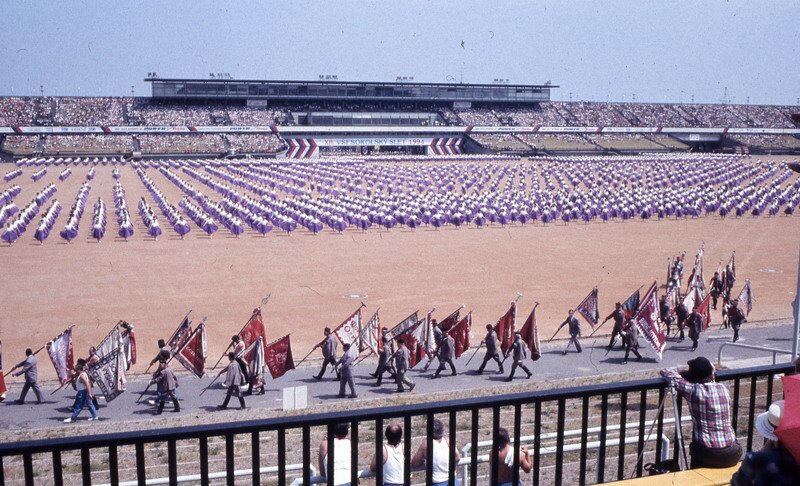
\includegraphics[width=0.9\textwidth]{img/44_slet_strahov.jpg}
  \caption*{Momentka z~XII. všesokolského sletu 1994, posledního na velké
  strahovském stadionu, foto: archiv T.~J. Sokol Libeň}
\end{figure*}

V~týdnu před sletem staví JILM na louce u~studánky ukázkový sletový
tábor (stany, týpka, brána, stožár, kuchyně, zábradlí, latrína, \ldots{}).
Nejprve bylo od dubna do června 6 brigád s~opravou vybavení, sháněním
stavebního materiálu atd. a pak jsme od 25.~6. do 1.~7. tábor stavěli --
trávili jsme tam vždy celá odpoledne a večery po škole a zaměstnání --
bylo to opravdu náročné. Nejvíce hodin zde odpracovali: Žabák 85, Aleš
72, Jirkan, Vítek a Gösta 70, Jestík 69, Portos 66, Mišina 63, Tomáš a
Zdeněk 62, Doník 61 a Kubík 60. Pečlivou průvodkyní se ve sletovém týdnu
pro asi 400 návštěvníků stala Sabina Hašová.

Na Strahově (na velkém sletovém stadionu) pak opět cvičí všech 6 šestek
a k~tomu i všichni 3 náhradníci. Žádná jiná jednota neměla tolik žáků.
Cvičí i 12 mužů -- vesměs cvičitelů. Pro všechny to byl nečekaně silný
zážitek. V~průvodu jde 75 našich členů v~krojích či cvičebním úboru a
také 3 naše prapory -- členský, žákovský a dorostenecký. Na Strahově
cvičilo 43 žákyň a žen, 6 párů rodičů s~dětmi a 51 žáků a mužů -- celkem
106 cvičenců.

Po sletě se konal v~ukázkovém táboře zakončovací posletový táborák a
Zdeněk Lauschmann (\pozned{náčelník, pozn. ed.}) oznámil, že v~Libni
doopravdy končí -- už před rokem se přestěhoval na Barrandov a dojíždění
je neúnosné -- vydržel jen kvůli sletu. Ptá se mě (Jirkana) jako
nejstaršího z~cvičitelů, jestli převezmu jeho štafetu. Kdybych tak
věděl, co to podání ruky bude znamenat!

Ve sletovém roce bylo zapsáno 113 žáků a dorostenců. Jednota má 896
členů. O~prázdninách 1993 se brousí a lakují parkety ve Velkém sále.
A~na konci roku 1994 má jednota již 976 členů. 10.~2. 1995 se koná valná
hromada, na které se Jiří "Jirkan" Novák stává náčelníkem.

\subsection{Šibřinky}

18.~února 1995 se po dlouhé době 47 let konají v~sokolovně šibřinky.
Odpoledne maškarní pro děti s~hudbou, tancem, vyhlášením nejlepších
masek a soutěžemi; večer pak taneční zábava pro dospělé. Šibřinky se
postupně staly vyhledávanou akcí. Dětí chodí pravidelně přes 100 a
naprostá většina z~nich v~maskách. Na večerní dospělácké bylo těch 350
až 400 lístků vždy rychle rozebráno. Pro nás (žáky a cvičitele) to
znamená vystěhovat nářadí, přivézt a připravit 100 stolů a 400 židlí,
\begin{figure*}[h!]
  \centering 
  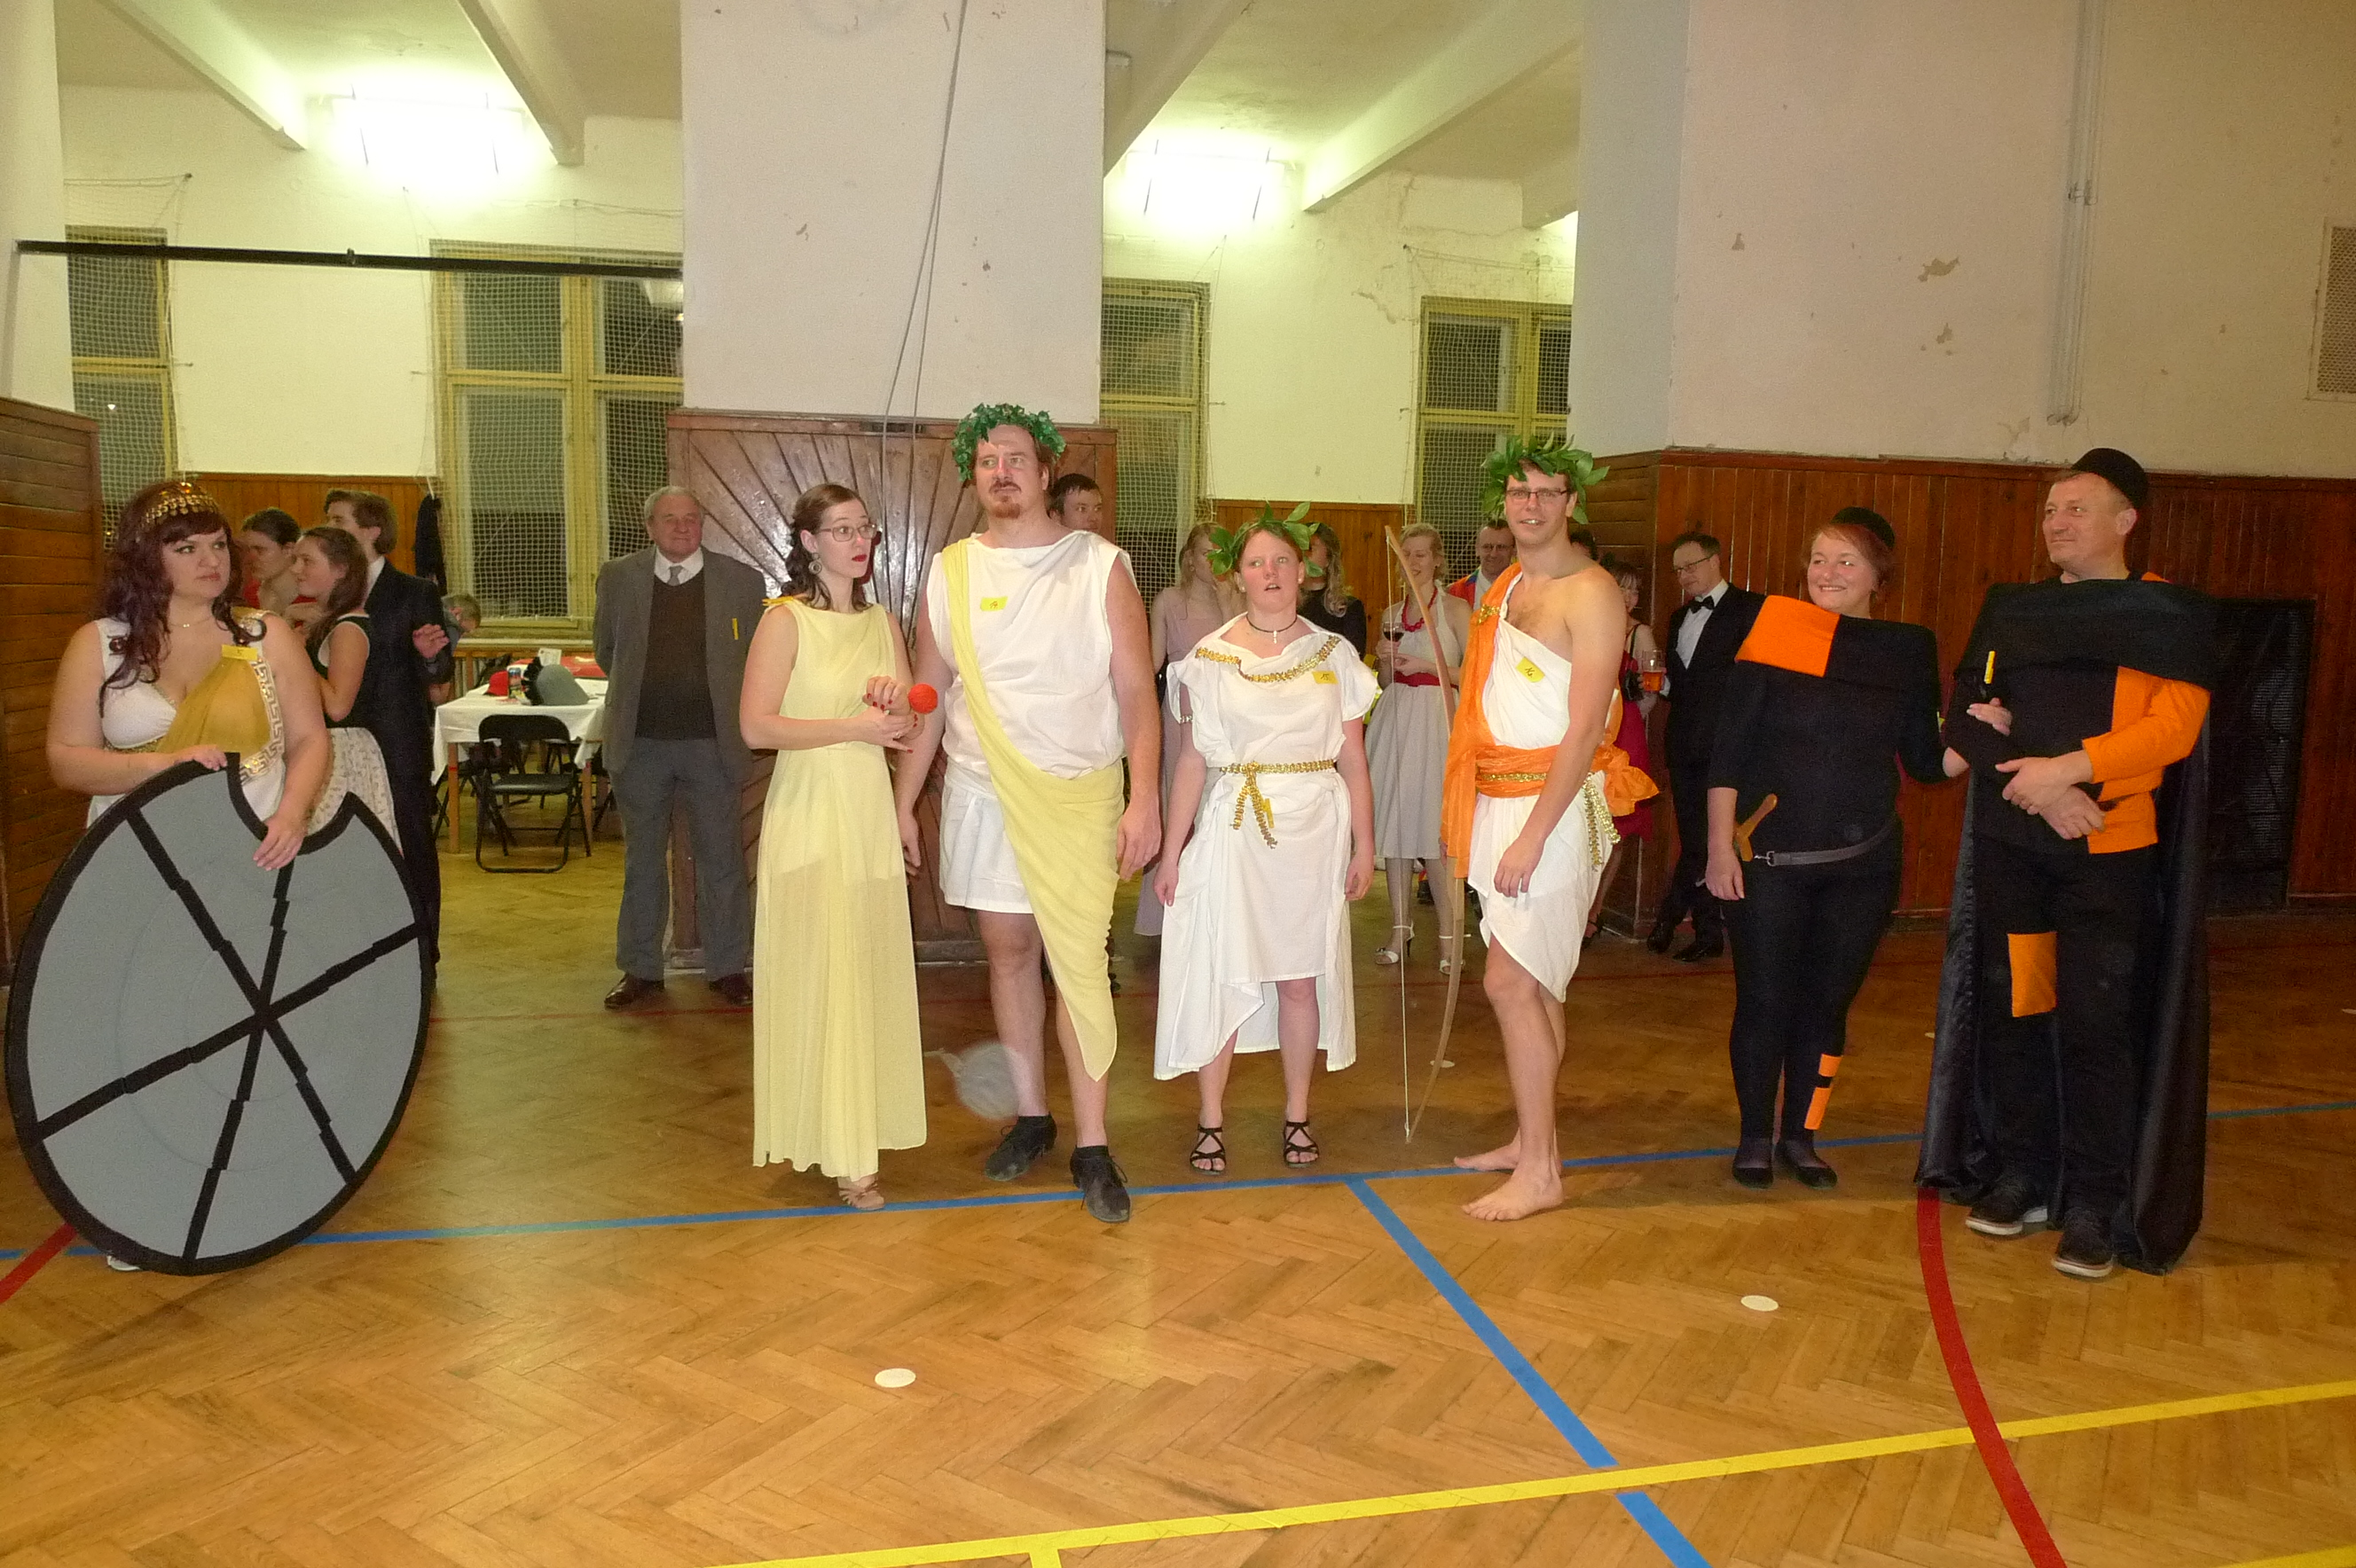
\includegraphics[width=0.9\textwidth]{img/45_sibrinky.JPG}
  \caption*{Šibřinky 2018 na téma staré pověsti české, foto: archiv J. Přecha}
\end{figure*}
večer obsadit šatnu a druhý den pak vše zase uklidit. Vlastní starost
o~program (předtančení, kapelu apod.) a o~občerstvení a obsluhu má
v~průběhu 90. let oddíl Studánka, jemuž při prodeji pomáhají i některé
členky Věrné gardy.

Tradice šibřinek nám také vydržela až do dnešních dní. Postupně se staly
z~akce pro veřejnost akcí pro členy a příznivce (\pozned{došli jsme
k~závěru, že práce s~dovozem stolů a židlí ze školy na Balabence a
zpřísňující se předpisy, které bylo třeba na veřejné akci plnit, již
nestojí za vydělané peníze, pozn. ed.}), avšak téma večera, živá kapela,
občerstvení, tombola, soutěž masek, předtančení a další vystoupení
zůstaly zachovány. Cvičitelstvo vše připraví, má služby během šibřinek a
v~neděli vše uklidí. Stále chodí 100--150 lidí. Současně se konají i
Dětské šibřinky, které mají své pohádkové průvodce, vystoupení, křepčení
na hudbu a v~druhé části soutěže s~odměnou. I~tady nám covid odvál
dospělácké šibřinky v~roce 2021 a dětské v~roce 2021 a 2022.

\subsection{Střípky z~90. let}

V~květnu 1995 se konají oslavy 50. výročí osvobození Plzně. Součástí
oslav jsou i sokolské slavnosti, kam s~loňskou sletovou skladbou jede i
12 libeňských žáků.

Na počátku roku 1996 má jednota už 1\,188 členů a je jednou z~největších
v~Praze. V~tomtéž roce slaví František Kodl 85 let.

Na podzim roku 1996 začal pracovat oddíl Sportovní gymnastiky, který si
pod vedením Martina Práta, Zuzany Lechnýřové a později Jiřího Hrňáka za
6~let svého působení dokázal vychovat závodníky a závodnice, kteří se
mohli měřit s~vrstevníky z~mnohem větších a dlouhodobě pracujících
oddílů. Oddíl se pak bohužel pro odchod trenérů v~roce 2002 rozpadl.

V~prosinci 1996 je poprvé poslední cvičební hodina žactva před vánočními
svátky zpestřena vystoupením našich loutkářů sdružených v~souboru
Vhlavědrát (více ve zvláštním článku). Jejich představení na vánoční
motivy jsou velmi pěkná a děti ani nedutají. Zvláště poslední
představení před Vánocemi 2003 bylo úžasné -- pohyblivé funkční kulisy,
živá hudba.

I~tradice vánočního loutkového představení se drží až do dnešních dnů.
Do roku 2014 a v~roce 2018 to byl "náš" soubor Vhlavědrát, v~letech
2015, 2016 a 2019 jsme si najali cizí soubory, v~době covidu (2020 a
2021) jsme poslali alespoň odkaz na hezkou vánoční pohádku a od roku
2022 nám hraje opět "náš" soubor, v~roce 2022 vzniklý Nástup!

V~létě 1996 byl restaurován originál obrazu Mikoláše Alše umístěný
v~Malém (badmintonovém) sále. Na popud Františka Kodla je tento sál
přejmenován na Alšův.

V~červnu 1998 se koná župní slet v~Brandýse nad Labem u~příležitosti
100. výročí vzniku župy Barákovy. V~zimě a na jaře pilně nacvičujeme, a
tak můžeme nabídnout 34 žáků (z~72 vystupujících) ve skladbě Správní
kluci. V~další skladbě -- Muž a žena -- cvičí 18 mužů.

V~roce 1998 umírá Fr. Kodl -- uprostřed neutuchající práce. Ještě pár
dní před smrtí připravoval vycházku Věrné gardy.

V~roce 1998 též vzniká z~"přestárlých" děvčat z~Káňat turistický oddíl
starších žákyň Pampelišky pod vedením Sabiny Hašové, dnes Pejsarové.
Káňata v~tu dobu vedou místo Sabiny Drb a Kačka (Tomáš Drbohlav a
Kateřina Fischerová). Pampelišky fungují (později pod názvem Mirek) do
roku 2002, kdy se částečně rozpadají, a zbytek se stává vedoucími Káňat
po odešlých Drbovi a Kačce. Káňata fungují stále. Vedoucími byla
postupně Ája, Vrečka a Zuzka Dočekalová, za které se dočkaly velkého
rozmachu (24 dětí na táboře), a nyní je vede Markéta Gottwaldová.
Postupem času se znovu zformoval turistický oddíl starších žákyň
s~názvem Veverky, který vedly mimo jiné Áďa nebo Liška. Při nedostatku
vedoucích se od září 2023 spojily s~oddílem JILM (více ve zvláštních
článcích).

Od podzimu 1998 do roku 2003 vypomáhají naši cvičitelé Vláďa Voráč a
Martin Chlumský při cvičení žactva v~jednotě Sokol Prosek a naši
cvičitelé a dorostenci se pravidelně v~sokolských krojích účastní
pietního aktu na Kobyliské střelnici.

Od jara 1999 má naše jednota také své internetové stránky. Pečlivě se
o~ně dodnes stará Vladislav Voráč -- možno se přesvědčit na www.sokol-liben.cz. Sám je také
spoluautorem a administrátorem informačního webu sokol.cz.

O~prázdninách 1999 byla sokolovna vyloupena. Bylo vylomeno přes 60 dveří
(i ty slepé, co kdysi vedly z~chodby do Srncova sálu), hodně věcí
ukradeno nebo rozbito. Ani jilmácká klubovna nezůstala ušetřena. Nic
cenného (pro ně) tam ti gauneři nenašli, a tak alespoň vše vyházeli na
zem. Uklízeli jsme to pak několik dní.

Koncem devadesátých let začala tradice zvaná Silvestr cvičitelů.
V~klubovně JILMu se vždy pár dní před koncem roku sejdeme, abychom
poklábosili, pobavili se, zazpívali si při kytaře nebo také domluvili
jarní výpravy či secvičili číslo na akademii. Postupně přibyli i hosté,
takže nás bývá okolo 25.

I~tato tradice přetrvává. Jen se místo konce roku scházíme až první
pátek roku nového. Program se nejprve nafoukl o~půlnoční odpalování
ohňostroje, ten však byl s~ohledem na restrikce opět zrušen. Jednou jsme
si v~rámci akce zahráli hokej, občas se sehraje zápas v~košíkové. Před
sletem se promítají sletové skladby, abychom věděli, co nás čeká.

\subsection{XIII. všesokolský slet 2000 --
Strahov}

Na podzim 1999 pak začíná nácvik na slet 2000. Mladší žáci mají skladbu
Sokolík se stavebnicí ze žlutých tyčí a modrých "bobků", starší žáci
mají společnou skladbu se žákyněmi v~rytmu rock and rollu (na hudbu
skupiny ABBA) a muži skladbu Chlapáci (\textit{která navazuje na podobnou
skladbu ze sletu 1994 a autorskou dvojicí Pavelka Dosedla bude ještě
několikrát recyklována, až skončí zcela nudná a vyprázdněná na sletu
2018, kdy ji naši muži odmítnou cvičit, pozn. ed}.). Myslím, že všechny
byly kvalitnější než v~roce 1994, avšak problémy s~nácvikem byly
podobné. Dokonce i počet cvičících se skoro nelišil. Po perném
osmiměsíčním nácviku se jilmácká osmička předvedla 17.~5. na akademii
v~Dolních Chabrech, nejilmácká pak o~pár dní později (20.~5.) na župním
sletě v~Roudnici. Obě společně pak 24.~5. na Pětižupní akademii v~hale
Sparty na Letné. Tam cvičili i muži. A~pak už Strahov. Nejprve má každá
skladba 2 až 3 secviky, pak generálku a nakonec sobotní a nedělní
vystoupení na Rošického stadionu. Byl to pro cvičitele opravdu zápřah.
Sami cvičili, navíc museli neustále přivážet či odvážet mladší či starší
žáky z~Palmovky na Strahov a zpět. Ale zvládli jsme to. I~přes obrovské
zmatky při neustálých změnách. Na Strahově cvičilo 26 mladších žáků (3
osmičky a dva další byli součástí osmičky Proseka), dále 15 starších
žáků s~jedním hochem z~Kobylis a také 17 mužů, kde nás na 18 doplnil
Zdeněk Lauschmann. Je jen škoda, že z~novinky tohoto sletu -- Národního
večera za umělého osvětlení bylo na poslední chvíli vyškrtnuto
vystoupení staršího žactva. Určitě by to pro ně byl jedinečný zážitek.
Nesmíme samozřejmě zapomenout na sletový průvod, večerní zakončovací
posletový táborák, na nějž cvičitelé připravili překvapení -- pro všech
117 libeňských účastníků sletu (cvičily i žákyně, R+D, Věrná garda a
další) nechali vyrobit krásné pamětní medaile. Nikdo jiný na světě
takovou nemá. Kromě toho proběhlo v~listopadu společné focení účastníků
sletu a také se promítalo video ze sletu -- každý se rád podíval, jak
vlastně vypadala jeho skladba z~pohledu diváka.

\subsection{Běh strmý}

Další tradice vznikla na podzim 2000. V~parku jsme uspořádali 0. ročník
Běhu strmého do zámeckého vrchu. Na trati dlouhé 199 metrů, s~převýšením
29 metrů se za deště sešlo 43 odvážlivců, kteří se rozhodli vyběhnout od
můstku do loděnic (dnes od povodňové zdi) serpentinami až na vrchol
kopce nad volejbalovými kurty. Soutěží se celkem v~11 kategoriích dle
věku. Pro vítěze je připraven nádherný putovní pohár -- ale protože je
vítězů 11, je pohár stále v~sokolovně a jména vítězů jsou vyrývána do
podstavce. Kromě toho vítěz obdrží plastiku sokolíka a diplom a každý
účastník pak pamětní lísteček.

Jednou jsme kvůli výstavbě protipovodňových zábran museli přesunout běh
na náhradní trať od dětského hřiště, podél šikmé louky na plošinku. Také
jsme s~postupem doby museli o~kousek posunout místo startu a cíle,
abychom dole nekřížili cestu cyklistům a lidem na procházce. A~změnou
prošla i hlavní trofej, cínová plastika sokolíka. Tu jsme nejprve
nakupovali od výrobce od Liberce. Po skončení výroby jsem si vyrobil
vlastní model na odlévání a asi 10 let jsme si je odlévali sami. Doba
však postupuje, a tak nám letos krásné (plastové) sokolíky na 3D
tiskárně zhotovil Ledňáček.

\vspace*{\baselineskip}
\noindent
Zde je přehled o~účasti a hlavním vítězi napříč kategoriemi:
%TODO nelíbí se mezera? Sekundy? (napříč)?
\begin{longtable}[]{%
  >{\raggedright\arraybackslash}p{1cm}%
  >{\raggedright\arraybackslash}p{1.2cm}%
  >{\raggedright\arraybackslash}p{1.2cm}%
  >{\raggedright\arraybackslash}p{1cm}%
  >{\raggedright\arraybackslash}p{4.5cm}}
\textbf{Ročník} & \textbf{Rok} & \textbf{Celkem běžců} & \textbf{Vítězný čas [s]} & \textbf{Absolutní vítěz (napříč~kategoriemi)} \\
\hline \endhead
0. & 2000 & 43 & 42,5 & Lukáš Pazdera – dorostenec \\
1. & 2001 & 59 & 40,2 & Jan Kaše – muž \\
2. & 2002 & 67 & 40,9 & Jan Kaše – muž \\
3. & 2003 & 109 & 41,1 & Jan Kaše – muž \\
4. & 2004 & 59 & 43,2 & Jan Hudský – muž \\
5. & 2005 & 122 & 40,4 & Jan Hudský – muž \\
6. & 2006 & 154 & 37,5 & Robert Čepek – muž \\
7. & 2007 & 156 & 38,7 & Jan Hudský – muž \\
8. & 2008 & 180 & 39 & František Juhász – muž \\
9. & 2009 & 166 & 38,8 & Jakub Kudroň – muž \\
10. & 2010 & 171 & 39 & Jakub Kudroň – muž \\
11. & 2011 & 144 & 38,9 & Jan Hudský – muž \\
12. & 2012 & 160 & 38,6 & Vladimír Parásek – muž \\
13. & 2013 & 120 & 39,8 & Jan Hudský – muž \\
14. & 2014 & 181 & 40 & Jan Hudský – muž \\
15. & 2015 & 159 & 42 & Martin Kubů – muž \\
16. & 2016 & 162 & 37,3 & Tomáš Nushart – muž \\
17. & 2017 & 116 & 38,2 & Ondřej Fojtík – muž \\
18. & 2018 & 155 & 38,8 & Dan Unzeitig – muž \\
19. & 2019 & 175 & 36,4 & Tomáš Nushart – muž \\
20. & 2020 & 194 & 36,6 & Vojtěch Paleta – dorostenec \\
21. & 2021 & 200 & 36,3 & Ondřej Paleta – muž \\
22. & 2022 & 180 & 38,8 & Vojtěch Paleta – muž \\
23. & 2023 & 204 & 38,6 & Vojtěch Paleta – muž \\
24. & 2024 & 179 & 38,7 & Vojtěch Paleta – muž \\
\end{longtable}

\subsection{Rekonstrukce fasády
sokolovny}

\begin{center}
  \textit{doplněno ze zprávy hospodářky 2004 Ivy Duchačové}
\end{center}

Libeňskou sokolovnu jsme od T.~J. Meteor Praha 8 převzali ve velmi
špatném stavu. Hygienička nám nedala povolení k~provozu a vytkla
nedostatky. Díky předem zaplacenému nájmu prvního nájemce DIREKTA, a.
s., ve výši 250\,000\,Kč a získání dalších nájemců (tiskárny ADALBERT a~SAZKA) jsme sokolovnu nechali vymalovat, vyčistit parkety a natřít,
rovněž vymalovat schodiště. Po prohlídce hygienika jsme dostali povolení
k~provozu a mohli získat pronájem tělocvičen školám.

Sokolovna byla i nadále ve velmi špatném stavu. Byla provedena
provizorní oprava střech a zahájeno jednání o~finančních dotacích na
opravu fasády, která byla v~havarijním stavu.

Během zimy 2000/2001 se podařilo získat grant na rekonstrukci vnějšího
pláště sokolovny. Byla nám prostřednictvím ČOS přislíbena dotace ve výši\newline
2\,800\,000\,Kč na opravu a rekonstrukci pláště sokolovny. Abychom dotaci
mohli získat, museli jsme ale stále doplnit z~vlastních prostředků 1\,200\,000\,Kč. Kde však vzít tak velké peníze?

Současně jsme hledali pomocí výběrového řízení firmu na opravu omítky,
kde vyhrála firma PSP-GDS. Dále jsme také hledali kupce na odprodej
Sokolích bud. Marně. Nakonec se firma PSP-GDS nabídla, že naše Sokolí
boudy i s~přilehlými pozemky odkoupí za 2\,500\,000\,Kč. Souhlasili jsme.
Jako malá, ale přece jen nějaká pomoc se ukázala být dotace od MČ Praha
8 -- 50\,000\,Kč.

Původní nabídka na opravu a rekonstrukci omítky naší sokolovny od firmy
PSP-GDS byla 3\,951\,000\,Kč bez DPH. Konečně mohla celá oprava začít a 4.~12. 2001 byla oprava a rekonstrukce pláště předána. ČOS zaplatilo za
předložené faktury 2\,800\,000\,Kč a po úspěšném prodeji Sokolích bud jsme
uhradili i zbývající část 1\,998\,297\,Kč. Celkem tedy oprava fasády přišla
na 4\,798\,297\,Kč. Protože se v~tu dobu už jednalo o~nemovitou kulturní
památku, je fasáda stejná (materiál, barevnost, členitost) jako v~roce
1910, kdy byla sokolovna dostavěna.

Byť již zvenčí krásná, nebyla naše sokolovna ještě v~pořádku. Chyběla
ještě nutná a okamžitá oprava střech. Opět jsme žádali o~granty,
tentokrát památkový úřad Magistrátu hl. m. Prahy a díky výborné přípravě
projektu jsme uspěli. Dne 17.~6. 2002 byla podepsána s~odd. památkové
péče smlouva na finanční příspěvek na obnovu nemovité památky ve výši 2\,860\,000\,Kč (\pozned{mám dojem, že jsou to jediné "památkářské peníze",
které jsme kdy dostali, pozn. ed.}). Po našich dřívějších výborných
zkušenostech převzala zakázku opět firma PSP-GDS. 1\,966\,227\,Kč byla
částka použitá na opravu střech, 1\,109\,856,70\,Kč jsme použili na opravu
vnitřních prostor sokolovny.

Zmíním zde 4 hlavní osoby, které se svojí činností zasloužily o~zdar
celého díla: starosta Josef Žáček, tajemník Jiří Sixta, jednatelka Marta
Halíková a náš odborný poradce z~řad cvičenců-mužů architekt Pavel
Jakoubek. Postupně se v~sokolovně opravuje i elektroinstalace,
rekonstruují se sprchy a záchody a opravuje střecha a na sokolovnu jsou
dosazeny krásné, nově vyrobené vývěsky.

Sokolovna se stává vyhledávanou budovou i mezi filmaři. Natáčí se nejen
v~sále, ale i ve Filipově síni, vybavené v~secesním slohu. Pro nás jen
dobře, neboť to vždy jsou dobře placené nájmy. Kromě toho se v~naší
tělocvičně konají i různé nácvičné srazy, školení a semináře pro
cvičitele.

\begin{figure*}[h!]
  \centering 
  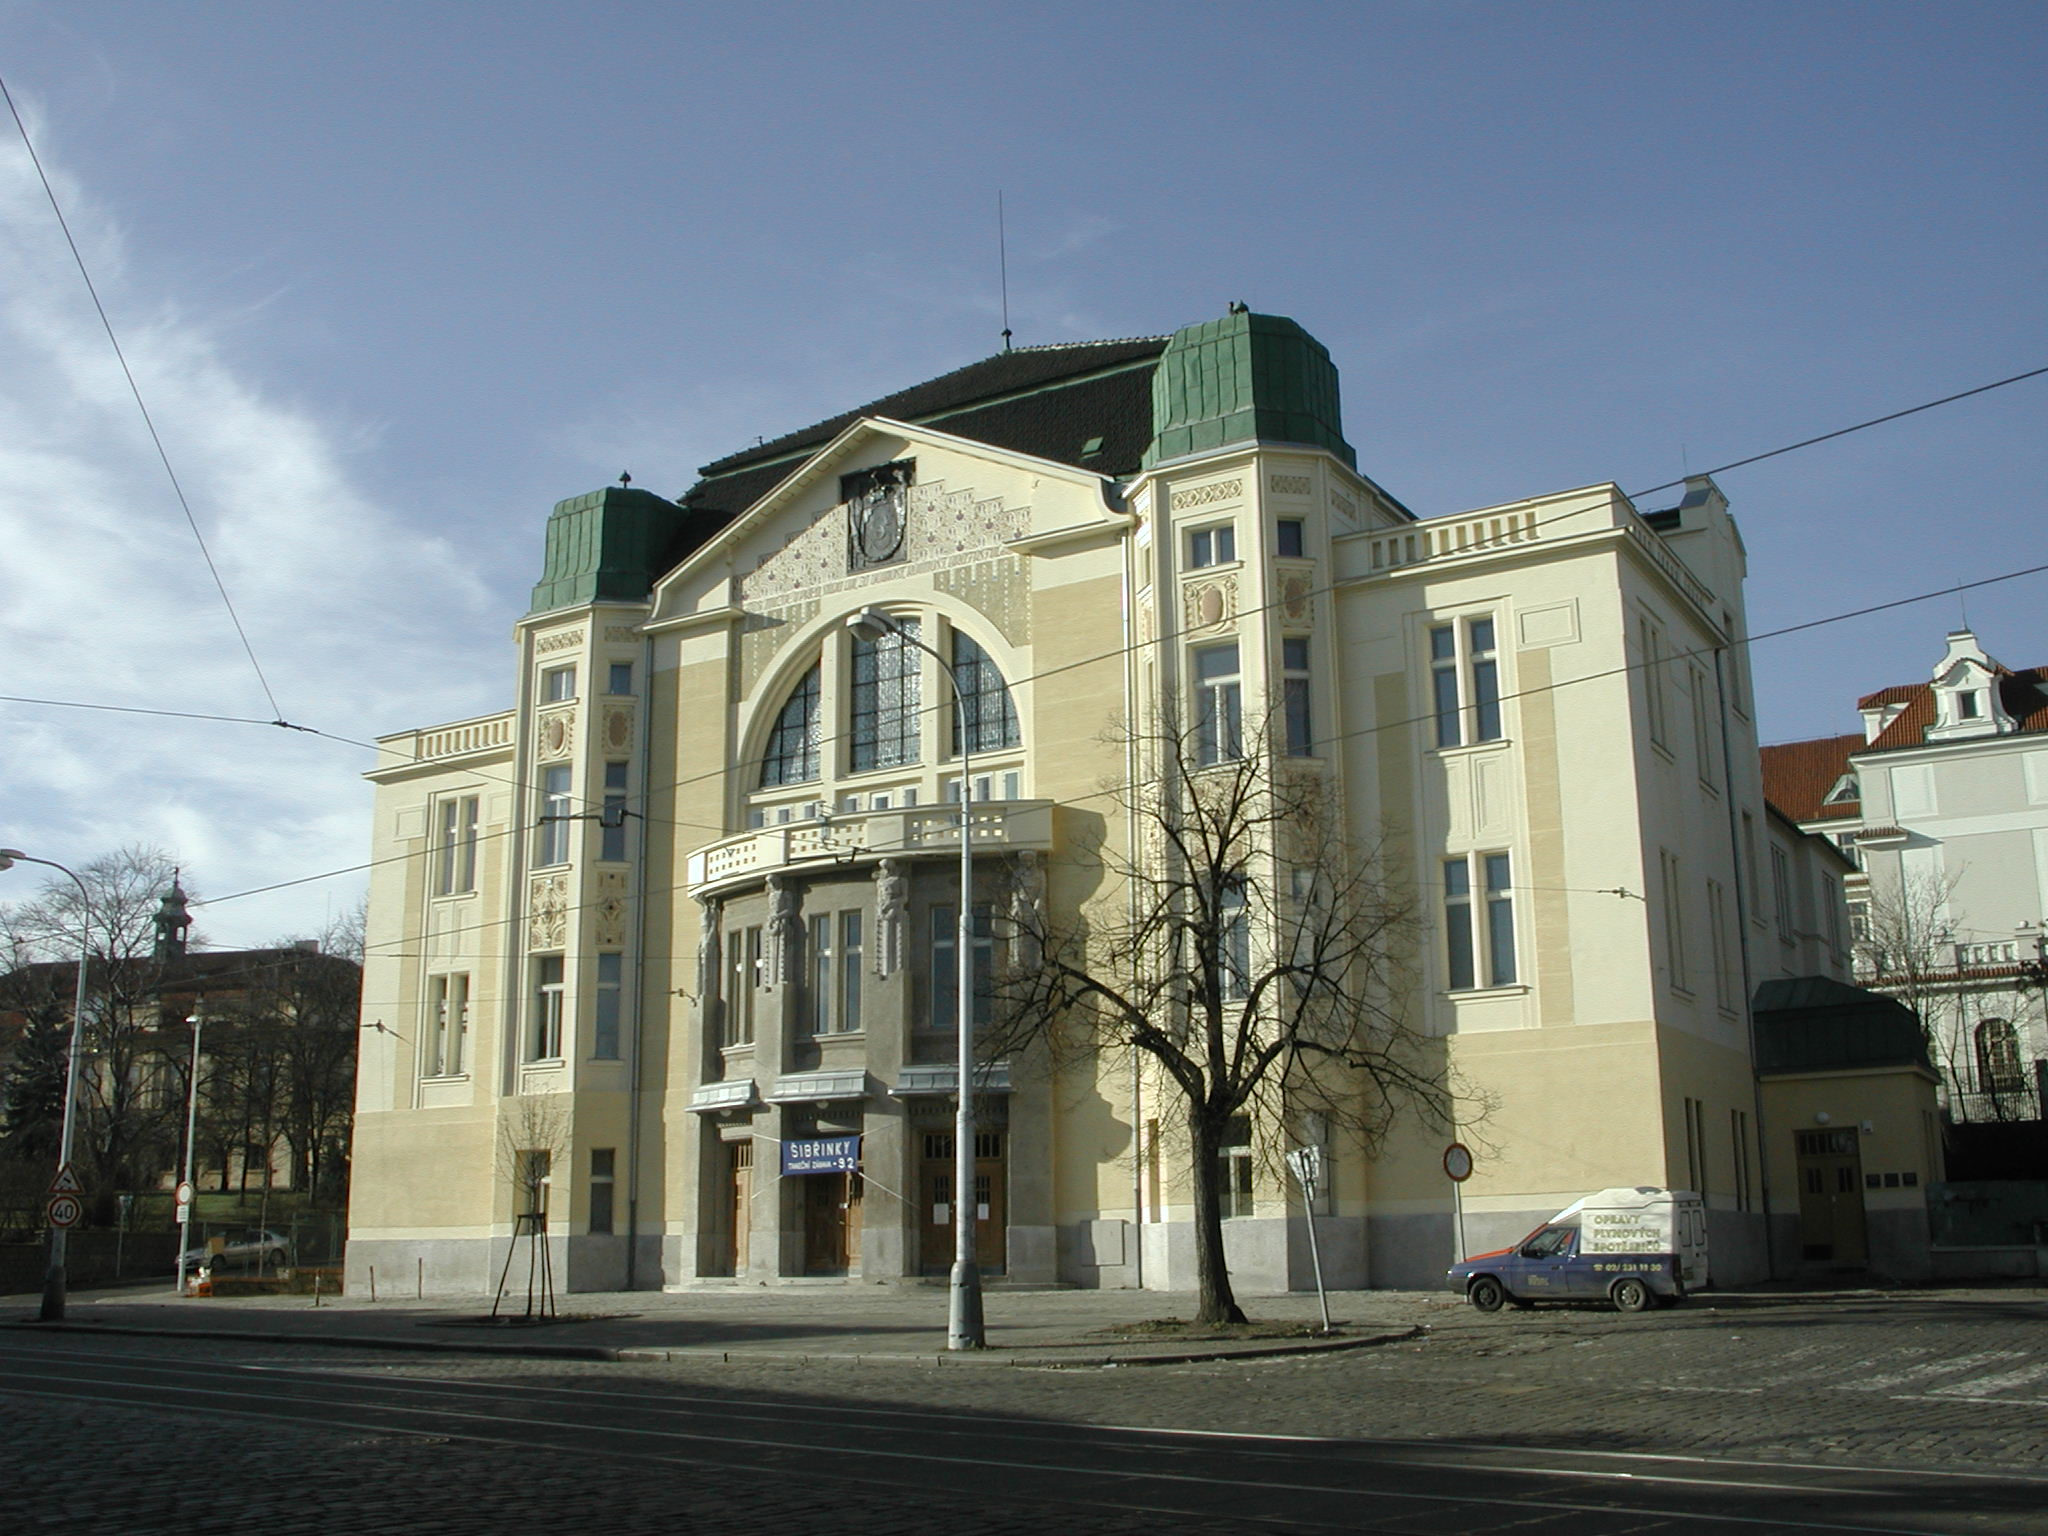
\includegraphics[width=0.9\textwidth]{img/46_sokolovna.jpg}
  \caption*{Sokolovna čerstvě po rekonstrukci (2002), foto: archiv T.~J. Sokol
  Libeň}
\end{figure*}

\clearpage

\subsection{Boj o~Sokolí boudy a práce Josefa Žáčka}

\begin{center}
  \textit{ze zprávy hospodářky 2004 Ivy Duchačové}
\end{center}

8.~4. 1991 k~nám přistoupil turistický oddíl Studánka s~vedoucím br.
Josefem Žáčkem, který se ihned zapojil do činnosti jednoty. V~roce 1992
se ujal řízení jednání i spolupráce na převzetí a opravách Sokolích bud
v~Dolní Malé Úpě, které jsme v~restituci převzali od Českých loděnic
Praha-Libeň. Zúčastnil se velmi složitých jednání jak o~Sokolí boudy,
tak i o~sokolovnu. V~roce 1994 jako jednatel, v~roce 1995 jako
místostarosta a v~roce 2001 jako starosta.

Abychom mohli doložit vlastní prostředky k~doplnění žádosti o~dotaci,
kterou jsme nutně potřebovali na opravu sokolovny, bylo rozhodnuto
o~prodeji Sokolích bud (13.~6. 1996 byl odsouhlasen ČOS). Kupec po
složitých jednáních nebyl nalezen, ale nabídl se p. Karlík, tehdejší
správce Sokolích bud, že tuto nemovitost i s~příslušnými pozemky
odkoupí. Měl však podmínku sepsání smlouvy, na kterou mu banka jedině
půjčí finanční prostředky.

Po poradě s~právním oddělením ČOS byla 10.~9. 1997 sepsána kupní smlouva
s~tím, že zaplatí 3\,450\,000\,Kč do 31.~3. 1998. Nezaplatí-li do tohoto
data, náleží právo prodávající straně od této smlouvy jednostranně
odstoupit. Účinnost odstoupení od smlouvy nastane dnem písemného
doručení druhé straně a tímto okamžikem se smlouva od počátku ruší. Pan
Karlík skutečně nezaplatil.

Zjistili jsme ale nedostatky v~našem právním řádu. Katastrální úřad
Trutnov požadoval na písemném doručení odstoupení od smlouvy podpis pana
Zdeňka Karlíka. Ten se však odmítl podepsat. Následoval soudní spor, ve
kterém nás zastupoval Mgr. Václav Čermák z~Trutnova. Mezitím byla 13.~8.
2001 Ministerstvem kultury prohlášena naše sokolovna za kulturní
památku. 13.~8. 2001 nám byly po vleklém soudním sporu a složitých
jednáních Sokolí boudy opět vráceny. Všechna tato jednání řídil a tlačil
kupředu br. Josef Žáček, již jako starosta jednoty.

Přesto, že byl těžce nemocen, nenechal se od práce odradit a řídil i
výše zmíněnou opravu sokolovny a ještě v~červenci 2003 organizoval letní
tábor Studánka a se vší iniciativou se ho zúčastnil. Dne 10.~srpna 2003
však zákeřné chorobě podlehl ve věku nedožitých 45 let.

Zásluhou jeho obětavé a nezištné činnosti je naše dnešní sokolovna
ozdobou památkově chráněného území městské části Libeň. Čest jeho
památce!

\subsection{Střípky z~let
2000--2010}

V~roce 2001 se na podzim účastníme župního turnaje v~sálové kopané a na
jaře 2002 ve florbalu. Na podzim 2001 a 2003 se s~velkým úspěchem
vracíme ze soutěže Rychlý šplhoun pořádané Sokolem Kobylisy. Vítězství
máme v~jednotlivcích i mezi štafetami. Na tuto akci jednoty v~Kobylisích
docházíme stále a většinou se vracíme s~medailemi.

Na jaře 2002 se v~Brandýse koná sokolský den. Vystupuje tam 16 mladších
žáků se skladbou Sokolík, kterou žáci předvedli na lednové akademii.
Cvičí i 7 starších žáků a dorostenců (přeskoky) v~bloku ukázek ze
cvičení. Ve skladbě Chlapáci cvičí 4 muži. Kromě toho Jilmáci postavili
týpko a uspořádali v~něm a jeho okolí malou výstavu o~své činnosti.

V~červnu 2002 slaví v~plné síle 90. narozeniny Manka Kodlová.

V~srpnu 2002 přicházejí povodně. Sokolovna uniká o~centimetry -- voda se
zastavuje u~lip stojících před sokolovnou. Zaplavena kanalizací je pouze
kotelna. Bylo potěšitelné, že se několik cvičitelů a dorostenců
zajímalo, jak na tom sokolovna je a zda nemají přijít pomoci. Vítek a
Čedok pak byli pracovníky krizového centra v~Bohnicích. V~září se
zjistilo, že jsou mezi námi vyplavené rodiny. A~tak se začalo vybírat do
modrých povodňových kasiček (vybráno asi 15\,000\,Kč). Spolu s~výtěžkem
z~mikulášské taneční zábavy a částí výtěžku ze šibřinek jsme dali
dohromady 30\,000\,Kč, které jsme rovnoměrně rozdělili mezi 4 postižené
rodiny a jednoty v~Karlíně a Nižboru. Kromě toho u~nás celý rok zdarma
cvičili žáci ze školy na Zámečku, kterým povodeň zničila tělocvičny.

\begin{figure*}[h!]
  \centering 
  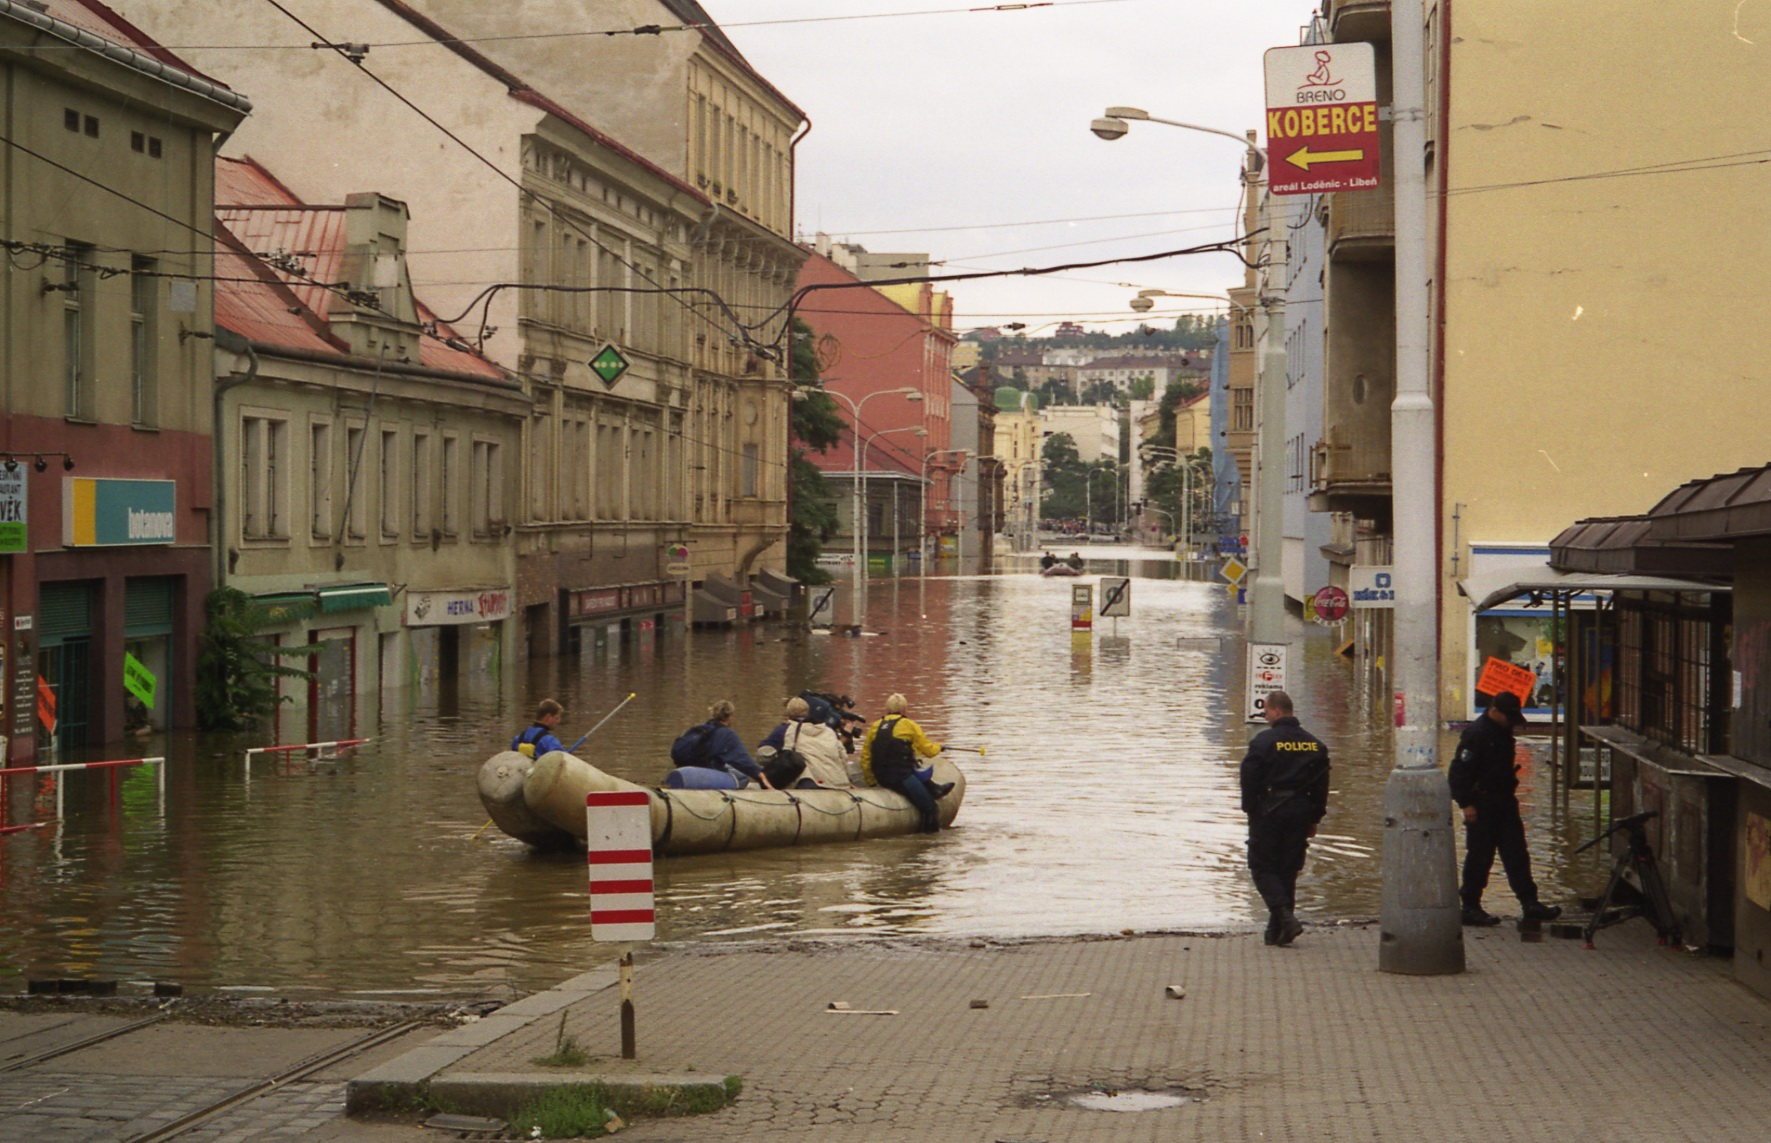
\includegraphics[width=0.9\textwidth]{img/47_povodne.jpg}
  \caption*{Povodně 2002, pohled z~Palmovky Zenklovou ulicí, foto: archiv T.
  J. Sokol Libeň}
\end{figure*}

{\sloppy V~srpnu 2003 nečekaně umírá v~necelých 45 letech starosta Josef Žáček,
agendu přebírá místostarosta Ladislav Mrklas ml. a po další valné
hromadě se starostou stává dosavadní tajemník Jiří Sixta. \par}

Od září 2003 získává dorost další hodinu -- je to úterý večer po cvičení
starších žáků. Tak jako se ve čtvrtek hraje košíková, hraje se v~úterý
florbal. Po několika letech se zájemci o~florbal přestali scházet a
z~úterní hodiny se stala hodina cvičitelská. Na každé hodině se probralo
jedno nářadí -- cviky, dopomoci, záchrana, přípravné cviky atd. Ale ani
tato náplň hodiny netrvala věčně a v~roce 2014 se stala hodinou pro
muže, jejichž cvičení obnovil Josef Kubišta (Pepišta). A~ti v~tuto dobu
cvičí v~hojném počtu dodnes.

K~1.~lednu 2004 má jednota 862 členů.

Počátkem roku 2004 umírá v~požehnaném věku 89 let také náš první
novodobý starosta Ladislav Mrklas st. (k~nalezení již na fotografii
cvičitelského sboru z~roku 1948, spolu s~Fr. Kodlem, strana 37). %ref cvicitele roku 48

V~souvislosti s~nadcházejícím sletem v~roce 2006 rozvířila Věrná garda
situaci kolem našeho historického praporu z~roku 1893. "Vždyť se ve
sletovém průvodu rozpadne! Chtělo by to nechat vyrobit repliku." A~hned
také začali po korunkách vybírat nutných 30\,000\,Kč. Pak padla myšlenka,
že by bylo hezké mít tu repliku už na slavnostní akademii ke 120.
výročí. Takže uzrálo rozhodnutí i ve mně. Přispějí i žáci. Prapor jsme
jim ukázali v~lednu 2004, mohli se podívat, sáhnout, a kdo chtěl, mohl
na jaře přispět (maximum bylo 50\,Kč). A~abych kluky trochu vyhecoval,
slíbil jsem, že co se vybere, to se sečte a tuto částku pak věnuji na
prapor sám. Bylo celkem 54 přispěvatelů a sešla se částka 3157,50, takže
na prapor bylo věnováno 6\,315\,Kč.

Zakončení cvičebního roku 2003/2004 s~vyhlášením Zimního klání a soutěže
O~nejvěrnější docházku jsme konali u~slavnostního táboráku. Pozvali jsme
i žákyně, cvičitelky, Věrnou gardu -- a sešlo se nás snad 100. Zpívalo
se, povídalo, rozdaly se diplomy a ceny a\ldots{} asi jsme založili další
tradiční akci. (\textit{Je to tak. Zakončovací táborák je jakýmsi milým
zakončením cvičebního roku, kdy se více oddílů sejde u~ohně, zazpívá
písničky, něco se sdělí přítomným rodičům, žáci si rozdají diplomky a
odměny za celoroční docházku a další soutěže, cvičitelé si po skončení
táboráku poklábosí mezi sebou, pozn. ed.})

O~prázdninách 2004 cvičitelé a Jilmáci za pomoci Jakuba Jabora ze
Studánky zbourali starou garáž, jež sloužila 10 let -- nejprve JILMu pro
uskladnění táborového vybavení, posléze jako loděnice. A~postavila se
nová, větší a hezčí loděnice (\textit{která bude zbourána během roku 2025,
aby ustoupila zvelebení prostoru za sokolovnou, pozn. ed.}).

Druhým vylepšením, které se událo o~prázdninách 2004, bylo přebroušení,
nalakování a nalajnování parket ve Velkém a Alšově sále a výměna povrchu
v~Srncově sále. Grant na tuto akci byl 400\,000\,Kč, náš doplatek 108\,000
Kč. Kéž oboje dobře slouží déle než 10 let. Nakonec došlo i na vstupní
dveře, které dělaly nové fasádě ostudu.

\subsection{Závěrem}

Tak, to jsem popsal tak 30\,\% naší činnosti. A~co je zbytek? No přece to
hlavní -- cvičení. Ale co o~něm psát? Jak skáčeme přes kozu, děláme
kotouly a celou gymnastiku, běháme, házíme, skáčeme a hrajeme hry. To
dost dobře nejde. Snad jen zmínit to, že se snažíme, aby kluci sobě
navzájem byli kamarády, pomáhali slabším, místo toho, aby se nad ně
vyvyšovali (za ty roky už u~nás cvičili i kluci po obrně, hluší,
s~cukrovkou, epileptici), aby vítězili vždy podle pravidel, aby jim bylo
ctí pomoci jako pořadatelé při Dětském dni (leckdy je u~soutěže jako
pořadatel i šikovný mladší žák), dokázali pomoci při věčném stěhování
nářadí, stolů a židlí při šibřinkách, chtěli vyhrávat na závodech, aby
dokázali myslet a dokázali odhadnout dopad svého jednání. Aby byli
ochotni přispět prací, ale třeba i drobně finančně (povodně, prapor),
aby naše sokolovna byla i jejich sokolovnou. A~aby se třeba časem stali
i cvičiteli. Aby z~nich prostě vyrostli lidé ochotní a přímí -- prostě
sokolové. Jsem rád, že se to daří. Jsem také rád, že i někteří naši
starší členové už pochopili, že pozdravem Nazdar, sestro/bratře, se
ještě nikdo sokolem nestal a že je důležité, co člověk dělá a jak to
dělá. Já jsem se naopak zase lecčemus přiučil od nich. Díky.

\medskip
\hfill\textit{Podzim 2004, částečně doplněno 2024}

\hfill\textit{Jiří Novák, 2004 náčelník, 2024 starosta}

\medskip
Průměrná docházka žactva a dorostu v~letech 1990--2024:
% TODO nelíbí se mezera?
\medskip
\renewcommand*{\arraystretch}{1.1}
\begin{longtable}[]{%
  >{\raggedright\arraybackslash}p{2cm}%
  >{\centering\arraybackslash}p{1.5cm}%
  >{\centering\arraybackslash}p{1.5cm}%
  >{\raggedright\arraybackslash}p{5cm}}
 \textbf{Rok} &  \textbf{Zapsáno} &  \textbf{Průměr} &  \textbf{Poznámka} \\
 \hline \endhead
 1990/1991 &  ? &  46 &  včetně mužů \\
 1991/1992 &  ? &  52 &  včetně mužů \\
 1992/1993 &  ? &  66 &  včetně mužů \\
 1993/1994 &  126 &  58,9 &  dále vždy ml. + st. žáci + dorostenci + cvičitelé (bez mužů) \\
 1994/1995 &  142 &  56,7 &    \\
 1995/1996 &  129 &  48,7 &    \\
 1996/1997 &  141 &  48,7 &  průměr v~říjnu 1996 je 71,55! (105~zapsaných) \\
 1997/1998 &  136 &  58,2 &  několikrát průměr 65–69, rekord~v~hodině 86! \\
 1998/1999 &  124 &  56,2 &    \\
 1999/2000 &  102 &  45,8 &    \\
 2000/2001 &  85 &  43 &    \\
 2001/2002 &  92 &  41,1 &    \\
 2002/2003 &  97 &  38,4 &    \\
 2003/2004 &  98 &  47,3 &    \\
 2004/2005 &  98 &  44,8 &    \\
 2005/2006 &  110 &  50,6 &    \\
 2006/2007 &  105 &  50,6 &    \\
 2007/2008 &  89 &  46,7 &    \\
 2008/2009 &  100 &  44 &    \\
 2009/2010 &  89 &  43,8 &    \\
 2010/2011 &  119 &  52,9 &    \\
 2011/2012 &  102 &  49,8 &    \\
 2012/2013 &  101 &  47,9 &    \\
 2013/2014 &  111 &  50,8 &    \\
 2014/2015 &  114 &  45,6 &    \\
 2015/2016 &  106 &  42,9 &    \\
 2016/2017 &  111 &  43,8 &    \\
 2017/2018 &  102 &  46,1 &    \\
 2018/2019 &  121 &  48,8 &    \\
 2019/2020 &  137 &  57,1 &    \\
 2020/2021 &  131 &  47,1 &    \\
 2021/2022 &  146 &  46,5 &    \\
 2022/2023 &  127 &  52,5 &    \\
 2023/2024 &  136 &  59,8 &    \\
\end{longtable}

\clearpage
A~kdo že se o~ty houfy kluků celé ty roky staral? Vezmu to podle
skutečného stáří (či spíše mládí); tabulka cvičitelů žactva
1990--2024:

\renewcommand*{\arraystretch}{1.1}
\begin{longtable}%
  {>{\raggedright\arraybackslash}p{3cm} %
  p{0.6cm} %
  >{\raggedright\arraybackslash}p{1.2cm} %
  >{\raggedright\arraybackslash}p{2.4cm} %
  >{\raggedright\arraybackslash}p{2.5cm}}

\textbf{Jméno} & \textbf{Rok nar.} & \textbf{Jak mu říkáme} & \textbf{Doba působení} & \textbf{Chodí ještě cvičit?} \\

\hline \endhead

Zdeněk Lauschmann & 1959 & Zdeněk & <1989–1994 & ne \\
Roman Kolář & 1965 & Roman & <1989–1993 & ne \\
Jiří Novák & 1970 & Jirkan & <1989– dosud & cvičitel, starosta \\
Filip Kadlec & 1971 & Filip & <1989–1997 & ne \\
Tomáš Novák & 1972 & Mišina & <1989– dosud & cvičitel \\
Jiří Materna & 1973 & Matýsek & 1993–1994 & ne \\
Tomáš Novotný & 1975 & Tomáš & 1993–1995 & ne \\
Petr Špírek & 1976 & Pierre & 1993–1997 & ne \\
Aleš Kafka & 1976 & Aleš & 1993–1994 & ne \\
Jan Hora & 1976 & Radík & 1993–1994 & ne \\
Vladislav Voráč & 1977 & Vláďa & 1993–2021 & Aerobik \\
Jiří Brůžek & 1978 & Jirka & 1997–1999 & ne \\
Jan Staněk & 1979 & Gösta & 1995–1997 & ne \\
Pavel Voráč & 1979 & Pavel & 1993–2013 & ne \\
Vít Jakoubek & 1979 & Vítek & 1995–2021 & výbor \\
Jan Turek & 1979 & Doník & 1996–2002 & ne \\
Jiří Hrňák & 1979 & Žabák & 1996–2000 & ne \\
Matěj Ištvánek & 1979 & Matěj & 1995–1997 & ne \\
Tomáš Jirsa & 1980 & Tomáš & 1995–1997 & ne \\
Jan Rejman & 1980 & Jarej & 1997–1998 & ne \\
Petr Bureš & 1981 & Petr & 1997–2002 & ne \\
Martin Chlumský & 1982 & Čedok & 1997–2018 & Aerobik \\
Pavel Jirsa & 1982 & Portos & 1998–2001 & ne \\
Matěj Beneš & 1983 & Benda & 1998–1999 & ne \\
Tomáš Seifert & 1985 & Tomáš & 2002 & ne \\
David Třešňák & 1985 & David & 2002 & ne \\
Martin Seifert & 1986 & Martin & 2002–2019 & ne \\
Jan Vorel & 1986 & Hnízdo & 2002–2007 & ne \\
Jan Veselý & 1980 & Honza & 2004–2025 & ne \\
Martin Kubů & 1983 & Sop & 2017–2021 & cvičitel PD \\
Michal Filipin & 1984 & Michal & 2004 & ne \\
Ondřej Fojtík & 1985 & Ondra & 2017–2019 & ne \\
Jan Dobis & 1985 & Honza & 2019–2020 & ne \\
Jan Přech & 1988 & Řek & 2004–2015 & jednatel \\
Jakub Kudroň & 1988 & Kubík & 2004–dosud & cvičitel \\
Jan Novák & 1989 & Pórek & 2005–2007 & ne \\
Jáchym Kaplan & 1990 & Jack & 2007–2017 & občas fotbálek \\
František Juhász & 1990 & Franta & 2007–2015 & košíková \\
Jan Dostál & 1990 & Sumec & 2007–2016 & Skipping Boys \\
Jiří Duchač & 1991 & Ruch & 2007–2016 & volejbal, výbor \\
Jan Přibyl & 1991 & Příbor & 2007–dosud & cvičitel, výbor \\
Ondřej Michalec & 1992 & Ondra & 2011–2016 & ne \\
Ondřej Loudil & 1992 & Hopi & 2008–2011 & cvičení mužů \\
Filip Benedikt & 1992 & Flip & 2008–2018 & ne \\
Marek Šťovíček & 1992 & Šťovík & 2008–2013 & ne \\
Josef Kubišta & 1992 & Pepišta & 2008– dosud & cvičitel, náčelník \\
Marek Vácha & 1992 & Marek & 2010–2011 & ne \\
Jan Slifka & 1992 & Slíva & 2010–2017 & košíková \\
Michal Přibyl & 1993 & Číba & 2010–2019 & občas košíková \\
Tomáš Mach & 1993 & Tomáš & 2010–2016 & ne \\
Lukáš Křemen & 1993 & Lukáš & 2019 & cvičení mužů \\
Ronald Eller & 1994 & Ronald & 2011 & ne \\
František Zima & 1997 & Franta & 2013 & ne \\
Ondřej Dvořák & 1997 & Ondra & 2013–2015 & ne \\
Martin Jeřábek & 1997 & Jestřáb & 2013–2014 & ne \\
Adam Cepník & 1998 & Adam & 2016–2017 & ne \\
Vojtěch Blahunek & 1999 & Blesk & 2014 & ne \\
Daniel Kadlec & 2000 & Daněk & 2015–2016 & vedoucí JILMu \\
Dan Unzeitig & 2000 & Kondor & 2016–2019, 2022 & vedoucí JILMu \\
Vojtěch Mrkvička & 2000 & Zelí & 2016–2017 & ne \\
David Hrnčiřík & 2001 & Hrnda & 2016 & ne \\
Richard Kloubský & 2001 & Ríša & 2017–2020 & cvičitel žákyň \\
Daniel Novotný & 2001 & Myslivec & 2017–2021 & ne \\
Jan Kerhart & 2002 & Kerhy & 2019–dosud & cvičitel \\
Petr Boháč & 2003 & Petr & 2019–dosud & cvičitel \\
Adam Novotný & 2003 & Adam & 2019–2021 & šplh \\
Jindřich Skokan & 2004 & Jindra & 2022–dosud & cvičitel \\
Tomáš Kléger & 2005 & Losos & 2022–dosud & cvičitel \\
Tomáš Ettel & 2006 & Timer & 2021 & šplh \\
Marek Novotný & 2006 & Marek & 2022 & šplh \\
Alexandre Basseville & 2007 & Padák & 2022–dosud & pomahatel \\
Jan Pikálek & 2007 & Ivánek & 2022–dosud & pomahatel \\
Václav Novák & 2008 & Vašek & 2023–dosud & pomahatel \\
Václav Blahunek & 2008 & Hrom & 2023–dosud & pomahatel \\
\end{longtable}

Byli samozřejmě ještě další, kteří si udělali alespoň pomahatelský kurs,
do skutečné cvičitelské práce se však nikdy pořádně nezapojili. My
budeme doufat, že čtyři dorostenci, kteří si dělají pomahatele tento
podzim, se zařadí do onoho výše uvedeného seznamu.

Všem těmto bratrům upřímný dík za sebe i za všechny cvičence, které kdy
něčemu naučili.

\begin{figure*}[h!]
  \centering 
  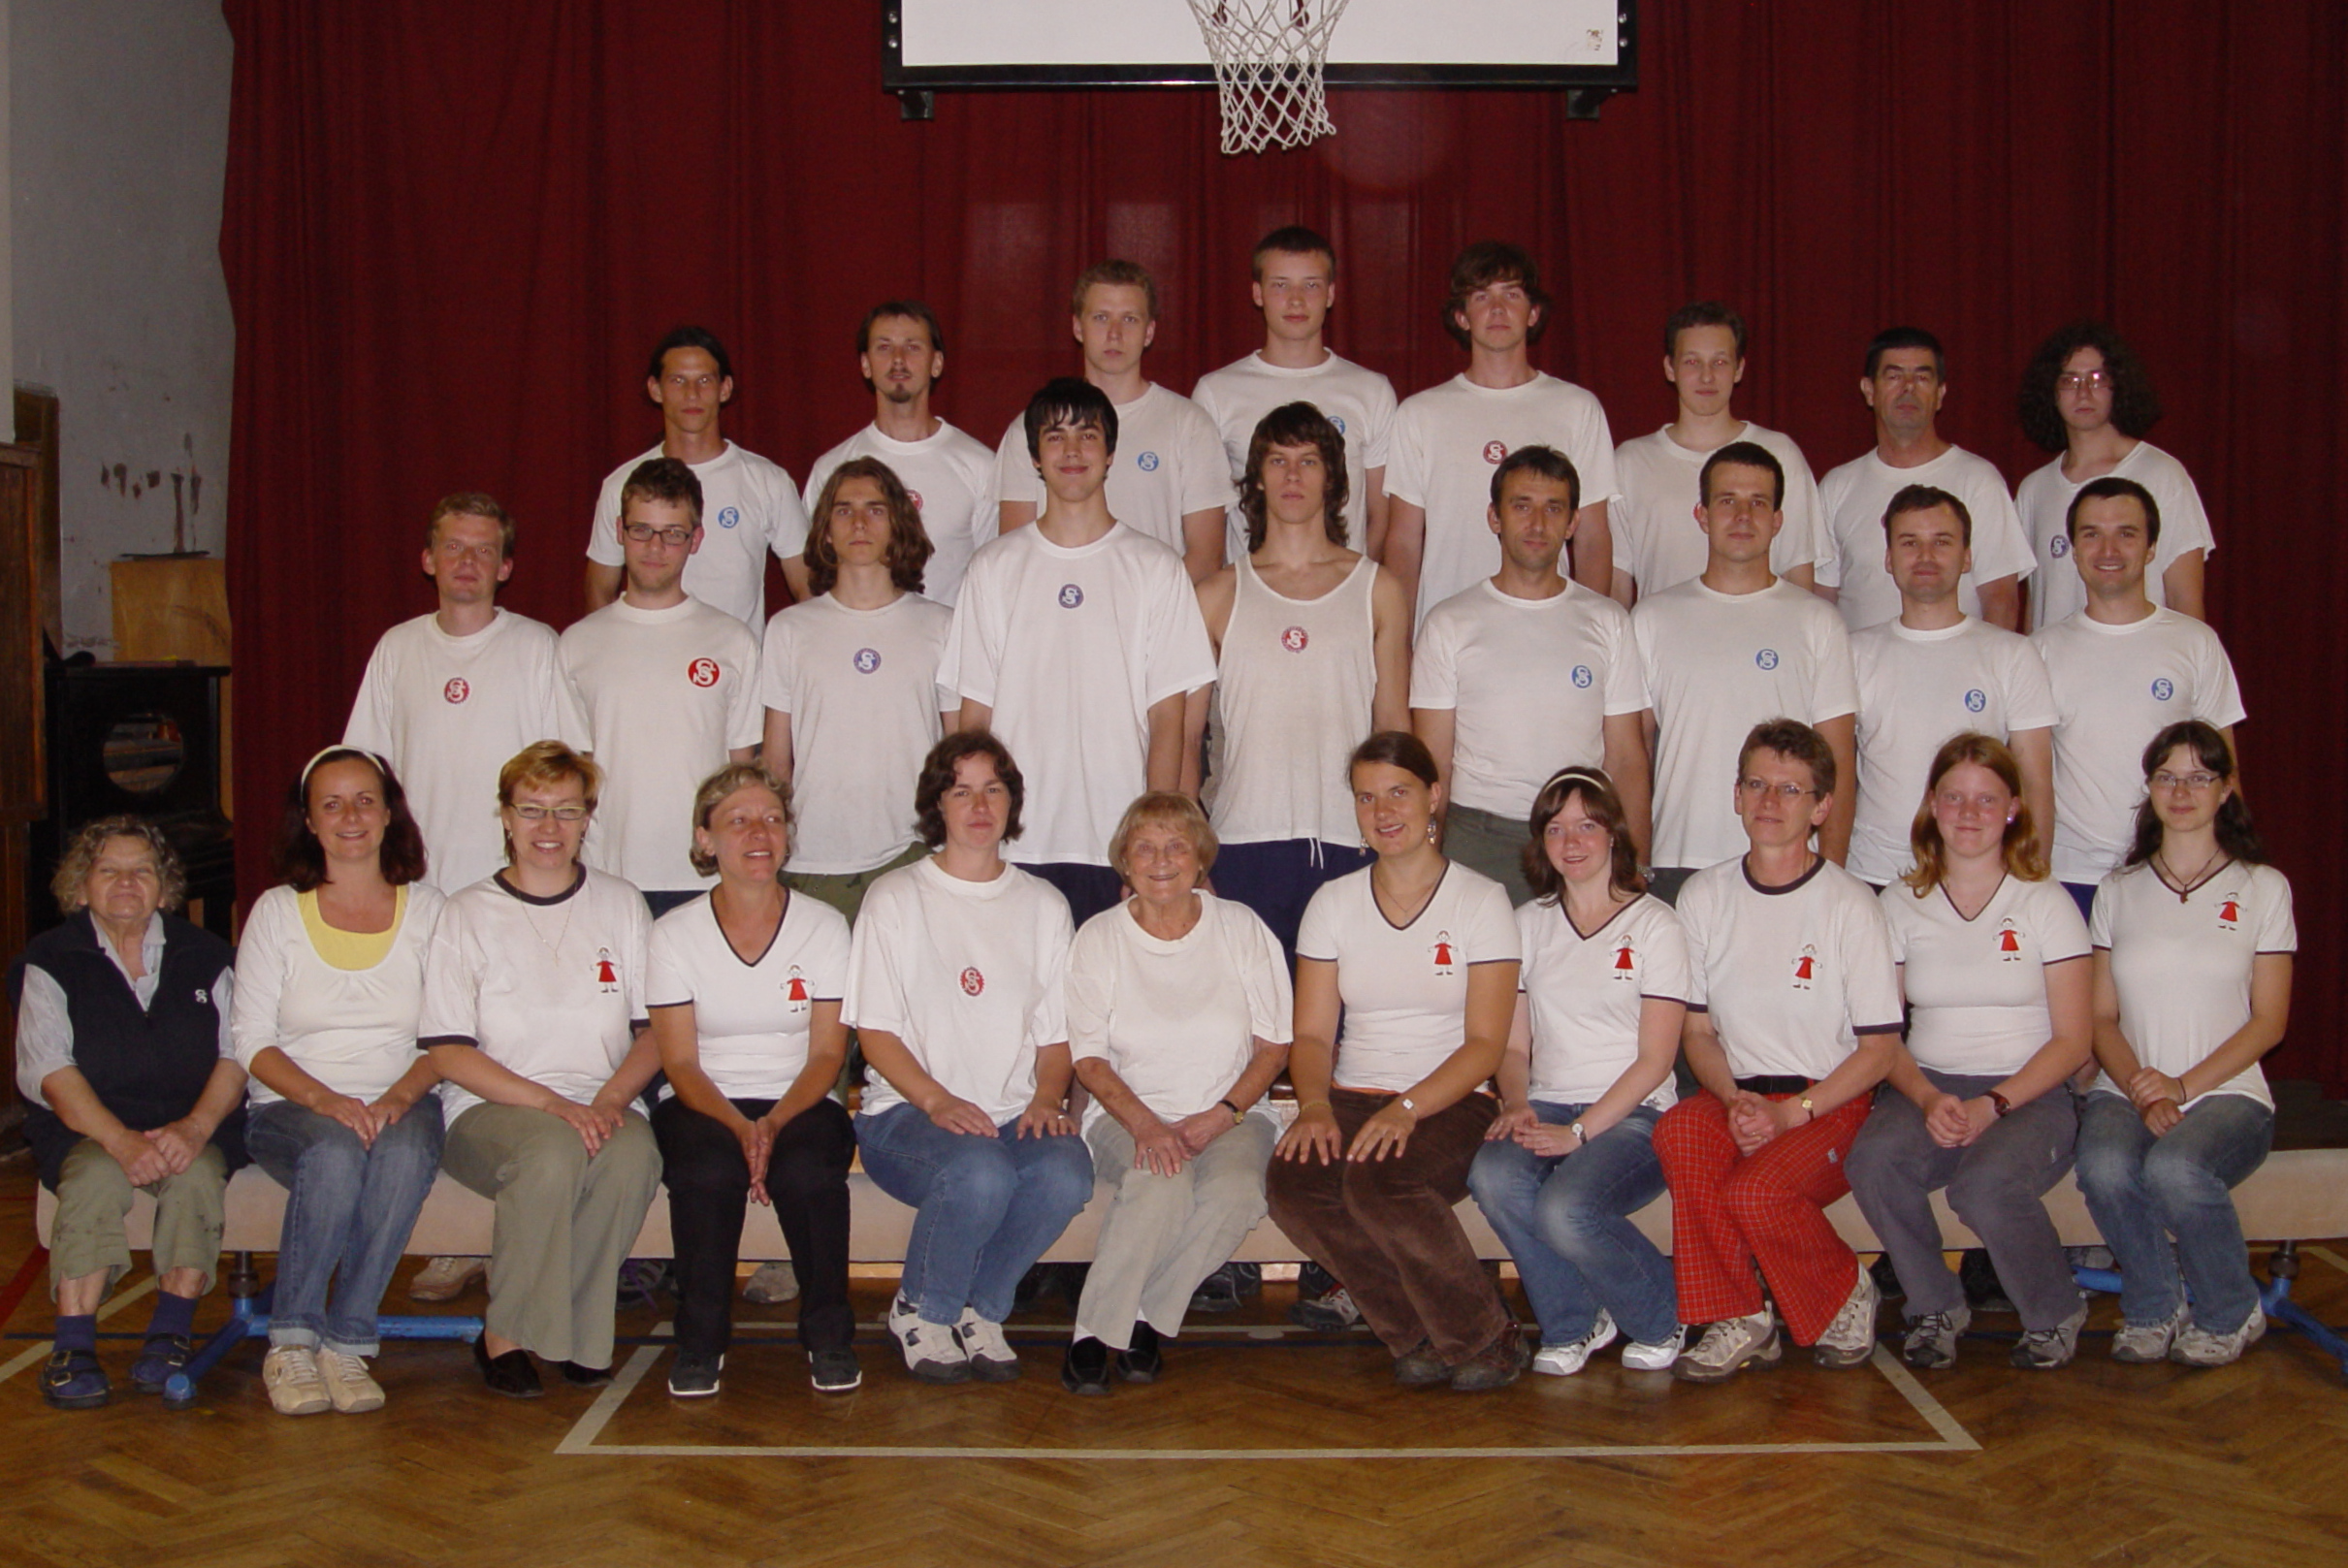
\includegraphics[width=0.9\textwidth]{img/48_cvicitele.JPG}
  \caption*{Cvičitelky a cvičitelé Sokola Libeň 2009: \\
  horní řada zleva: Jakub Kudroň, Tomáš Novák, Jan Dostál, Ondřej Loudil, Filip Benedikt, Jan
  Přech, Josef Maleček, Marek Šťovíček; \\
  střední řada zleva: Vít Jakoubek,
  Jan Novák, Josef Kubišta, Jan Přibyl, Martin Seifert, Jiří Novák (t. č.
  náčelník), František Juhász, Vladislav Voráč, Pavel Voráč; \\
  dolní řada
  zleva: Anna Kavinová, ?, Dana Blahunková, Anna Feřtová, Lenka Nováková,
  Evženie Hraničková, Zuzana Burianová, Lucie Vojáčková, Iva Duchačová,
  Alena Krásová, Veronika Niederlová, \\
  foto: archiv T.~J. Sokol Libeň}
\end{figure*}

\section{Slovo vzdělavatelky Věry Štastné
(2004)}

120. výročí založení sokolské jednoty Praha-Libeň, to znamená 120 let
sokolské práce, nadšení, krásy a radosti, ale v~tom celé roky byly také
plné smutku, bolesti a někdy i hrůzy a strachu o~milovaný Sokol. Nikdy
však nepřišla beznaděj, tu sokolové nikdy neznali, vždy věřili, bojovali
za svá práva a po spravedlnosti zvítězili.

Nová sokolská jednota, to byla nesmírná radost, doba nadějí a víry
v~sokolskou budoucnost a s~ní i v~budoucnost českého národa. Ze skromných
začátků Sokol sílil a po položení základního kamene ke stavbě sokolovny
v~roce 1909 už za 9 měsíců zazářila v~Libni nová sokolovna, která svou
venkovní i vnitřní architekturou se stala ozdobou centra Libně.
A~Tyršovým heslem v~průčelí nad balkonem provedeným ozdobným písmem
Mikolášem Alšem "Kupředu silou lví, za rovnost, volnost, bratrství"
jako by tušila, co všechno bude muset Sokol --⁠⁠⁠⁠⁠⁠ i libeňský Sokol a jeho
členové za těch 120 let prožít, kolik strastí a bolesti, ale i naděje.
Ale jejich vítězství vždy přišlo, krásné a nadějné.

Třikrát byla Sokolu pozastavena činnost, třikrát jsme se o~něj báli.
Sokolové platili krutou daň, ale nikdy ne zbytečně. Na druhou stranu
v~naší sokolovně celé generace prožívaly chvíle radosti při cvičení,
výletech, zájezdech, šibřinkách, různých veselicích či v~loutkovém
divadle. Trubačský sbor byl ozdobou všech vystoupení, výstavy vztahující
se k~činnosti jednoty byly spolu s~účastí na celonárodních shromážděních
dobrou ukázkou naší činnosti, to všechno cílilo k~národnímu uvědomění,
ale také k~rozvoji kulturního a společenského života. Poděkování patří
těm, kteří před námi tvořili historii libeňské jednoty a všechnu tu
krásu i památky uchovali pro nás i naše děti.

V~roce 1990 byl Sokol obnoven a také naše libeňská jednota se mohla
hlásit o~svůj majetek, svou krásnou sokolovnu i se cvičištěm vedle ní,
které nám však dosud vráceno nebylo.

Naše jednota má historii, na niž může být hrdá, jsou to vzpomínky krásné
i těžké, ale všechny vypovídají o~lásce k~vlasti, o~čestnosti, hrdosti i
hrdinství našich členů. Co přát naší jednotě k~tak nádhernému výročí?
Aby žila dále věrností k~sokolským ideálům svobody a demokracie, pravdou
a láskou k~vlasti a aby dále splňovala to, o~čem snily celé generace:
silný Sokol, věrné členy a hodně, hodně mládeže --⁠⁠⁠⁠⁠⁠ v~ní je naše
budoucnost, v~ni musíme, chceme věřit.

\clearpage

\section{Dění v~jednotě po roce 2004}

\begin{center}
  \textit{sepsal Jan Přech a Jiří Novák, převážně z~pohledu mužských složek}
\end{center}

\subsection{Úvodem}

Povídání shrnující dění v~naší jednotě za posledních 20 let začnu od
lidí. Mám pocit, že na ně máme štěstí. A~to jak na ty, kteří jsou vidět,
mají nějakou funkci, komunikují s~úřady, veřejností, rodiči, tak také na
ty, kteří tak vidět nejsou, ale bez nichž by naše snažení nebylo možné.
A~těch je většina. Jako cvičitelé velmi pravidelně a zodpovědně chodí
cvičit děti, po cvičení uklidí nářadí a zamknou skříně, na brigádách
podají pomocnou ruku při složitějších činnostech, neboť to jsou často
manuálně pracující lidé, jiní se starají o~vývěsky, další vytvářejí
diplomky, jsou schopni vytvořit pro naši jednotu matriční a platební
systém, jdou otevřít starším žákům během konce cvičení mladších,
v~turistických oddílech zastávají funkci pomocných vedoucích, vedou
některé z~našich tradičních akcí, vymýšlejí a počítají naše Zimní
soutěže a Letní disciplíny atd. Zkrátka vytvářejí podhoubí, ze kterého
pak může vyrašit naše rozmanitá, rozsáhlá a nápaditá činnost. Jim všem
patří mé upřímné poděkování za neocenitelnou pomoc. A~nemusí se jednat
o~lidi zkušené a starší. I~noví mladí pomahatelé ve svých patnácti či
šestnácti letech jsou pro ostatní zkušenější cvičitele velkou podporou.
A~to, že je občas zkritizují za nějaké špatné rozhodnutí, je jen známka
toho, že chtějí i přes ně pro cvičení to nejlepší. I~nynější starosta
České obce sokolské (ČOS) byl takto koncem devadesátých let peskován.
A~kam to dotáhl -- ale to je spíš jeho zásluha. I~když je možné, že nějaké
to semínko spolehlivosti, sebejistoty, přímého jednání, kamarádství,
vůle a dalších podobných vlastností v~něj i ve všechny ostatní cvičitele
a vedoucí oddílu bylo vloženo během cvičení a členství v~JILMu.

\hfill(\textit{br. Jiří Novák})


\subsection{Činovníci jednoty}

A~nyní k~těm, kteří vidět jsou. Máme mezi sebou držáky, kteří své břímě
a radost nesou většinou dlouhé roky a jsou tak zárukou kontinuity a
předvídatelnosti. Začněme starosty. Prvním po obnovení Sokola byl
Ladislav Mrklas starší (1990--2001). On byl tím, za jehož
starostování byla jednotě vrácena sokolovna a obnoveno cvičení, začala
jednání o~opravě fasády sokolovny. Dalším v~řadě byl Josef Žáček
(2001--2003), během jeho působení byla opravena fasáda
sokolovny a mám pocit, že byl přijat tajemník Jiří Sixta. Po úmrtí
Josefa Žáčka v~srpnu 2003 vedl jednotu místostarosta Ladislav Mrklas ml.
V~roce 2004 byl starostou zvolen Jiří Sixta (2004--2013),
který mimo jiné zařídil novou plynovou kotelnu, za jeho starostování se
znatelně zvýšila četnost žádostí o~granty, začalo pravidelné lakování
parket. Po devíti letech už nečekaně nekandidoval a my jsme řešili post
starosty. Nakonec padla volba na Nelibeňáka, ale člověka, kterého jsme
dobře znali. Byl jím bývalý náčelník Sokola Malešice a župní hospodář
Aleš Müller (2013--2019), který stál za sepsáním přání a
nápadů k~vylepšení a rekonstrukcí sokolovny (více o~něm dále). Za něj
začaly práce na studiích a projektech k~rekonstrukci dvora a šaten.
A~zatím posledním v~řadě je Jiří Novák (od 2019), který dotáhl k~realizaci
rekonstrukci šaten a započal stavbu nové podzemní místnosti (loděnice)
na dvoře a tím celkovou rekonstrukci dvora. Důležité také je, že všichni
tito starostové byli nakloněni a nápomocni k~realizaci různých vylepšení
a nápadů, se kterými přicházeli cvičitelé. Tak vzniklo v~roce 1995
doskočiště na dvoře, postupem doby osvětlení na akademii, různé
pravidelné akce (šibřinky, Dětský den, Běh strmý, Památný den sokolstva,
Den otevřených dveří, Silvestr cvičitelů, brigády, Zakončovací táborák,
\ldots), byl renovován Alšův sál, svépomocí vznikla hudební zkušebna
v~chodbě u~archivu a byla rekonstruována posilovna či postavena loděnice
za sokolovnou. V~poslední době byla postavena tahací věž či zakoupena
táborová louka pro turistické oddíly. Díky všem.

{\sloppy Dalšími viditelnými osobami jsou náčelník a náčelnice. U~děvčat to byla dlouho Věra Decastellová a následně Dana Blahunková, Alena Krásová a
v~současnosti Tomáš Dragoun. V~mužských složkách začnu už před rokem 1989,
kdy by asi byl náčelníkem František Kodl. Po obnovení Sokola pak už máme
pouze tři jména: Zdeněk Lauschmann (1990--2004), který již v~roce 1982
založil turistický oddíl JILM (sám jako dítě chodil přímo k~Foglarovi do
"skautského" oddílu Dvojka) a vedl 14 jilmáckých táborů a který po
Františku Kodlovi držel v~osmdesátých a devadesátých letech v~oddíle
ZRTV Meteoru Praha sokolský duch a který žáky a muže dovedl na první
sokolský slet po obnovení Sokola v~roce 1994. Jeho přínosem bylo také
zavedení kamarádství mezi kluky jako priorita chování. V~roce 1993 se
odstěhoval na Barrandov (ani tam však dlouho nezůstal bez Sokola a stal
se cvičitelem v~Sokole Zlíchov) a od roku 1994 přenechal náčelnictví
Jiřímu Novákovi (1994--2019). Ten navázal na Zdeňka
v~tradici výchovy nových cvičitelů z~vlastních zdrojů, tedy dorostenců, a
taky na to, že i žáci mohou být nápomocni při pořádání našich akcí a tím
se zároveň stávají důležitou součástí soukolí a jsou více vtaženi do
dění. Jirkan jako odchovanec JILMu byl taktéž mužem činů a dokázal tak
během brigád a dalších akcí posunout činnost na vyšší obtížnost
(doskočiště, dílna na nově zbudovaném trámovém patře v~bývalé kotelně,
nová loděnice, bourání starých garáží na dvoře). Koncem roku 2018 se po
25 letech ve funkci (a protože už vše běží bez invence jen tak
samospádem) domluvil s~Josefem Kubištou, že ten převezme náčelnictví a
on se stane jen řadovým cvičitelem. Jenže zemřel Aleš Müller a on byl
okolnostmi dotlačen stát se starostou. Josef Kubišta je tedy náčelníkem
od roku 2019 dosud. S~ním přišla opět mladická invence a entuziasmus.
Bylo obnoveno cvičení mužů, vznikly oddíly šplhu a přetahu lanem, vydal
přes ČOS Sokolské pohádky, vidí další práce k~vylepšení sokolovny.\par}

\begin{figure*}[h!]
  \centering 
  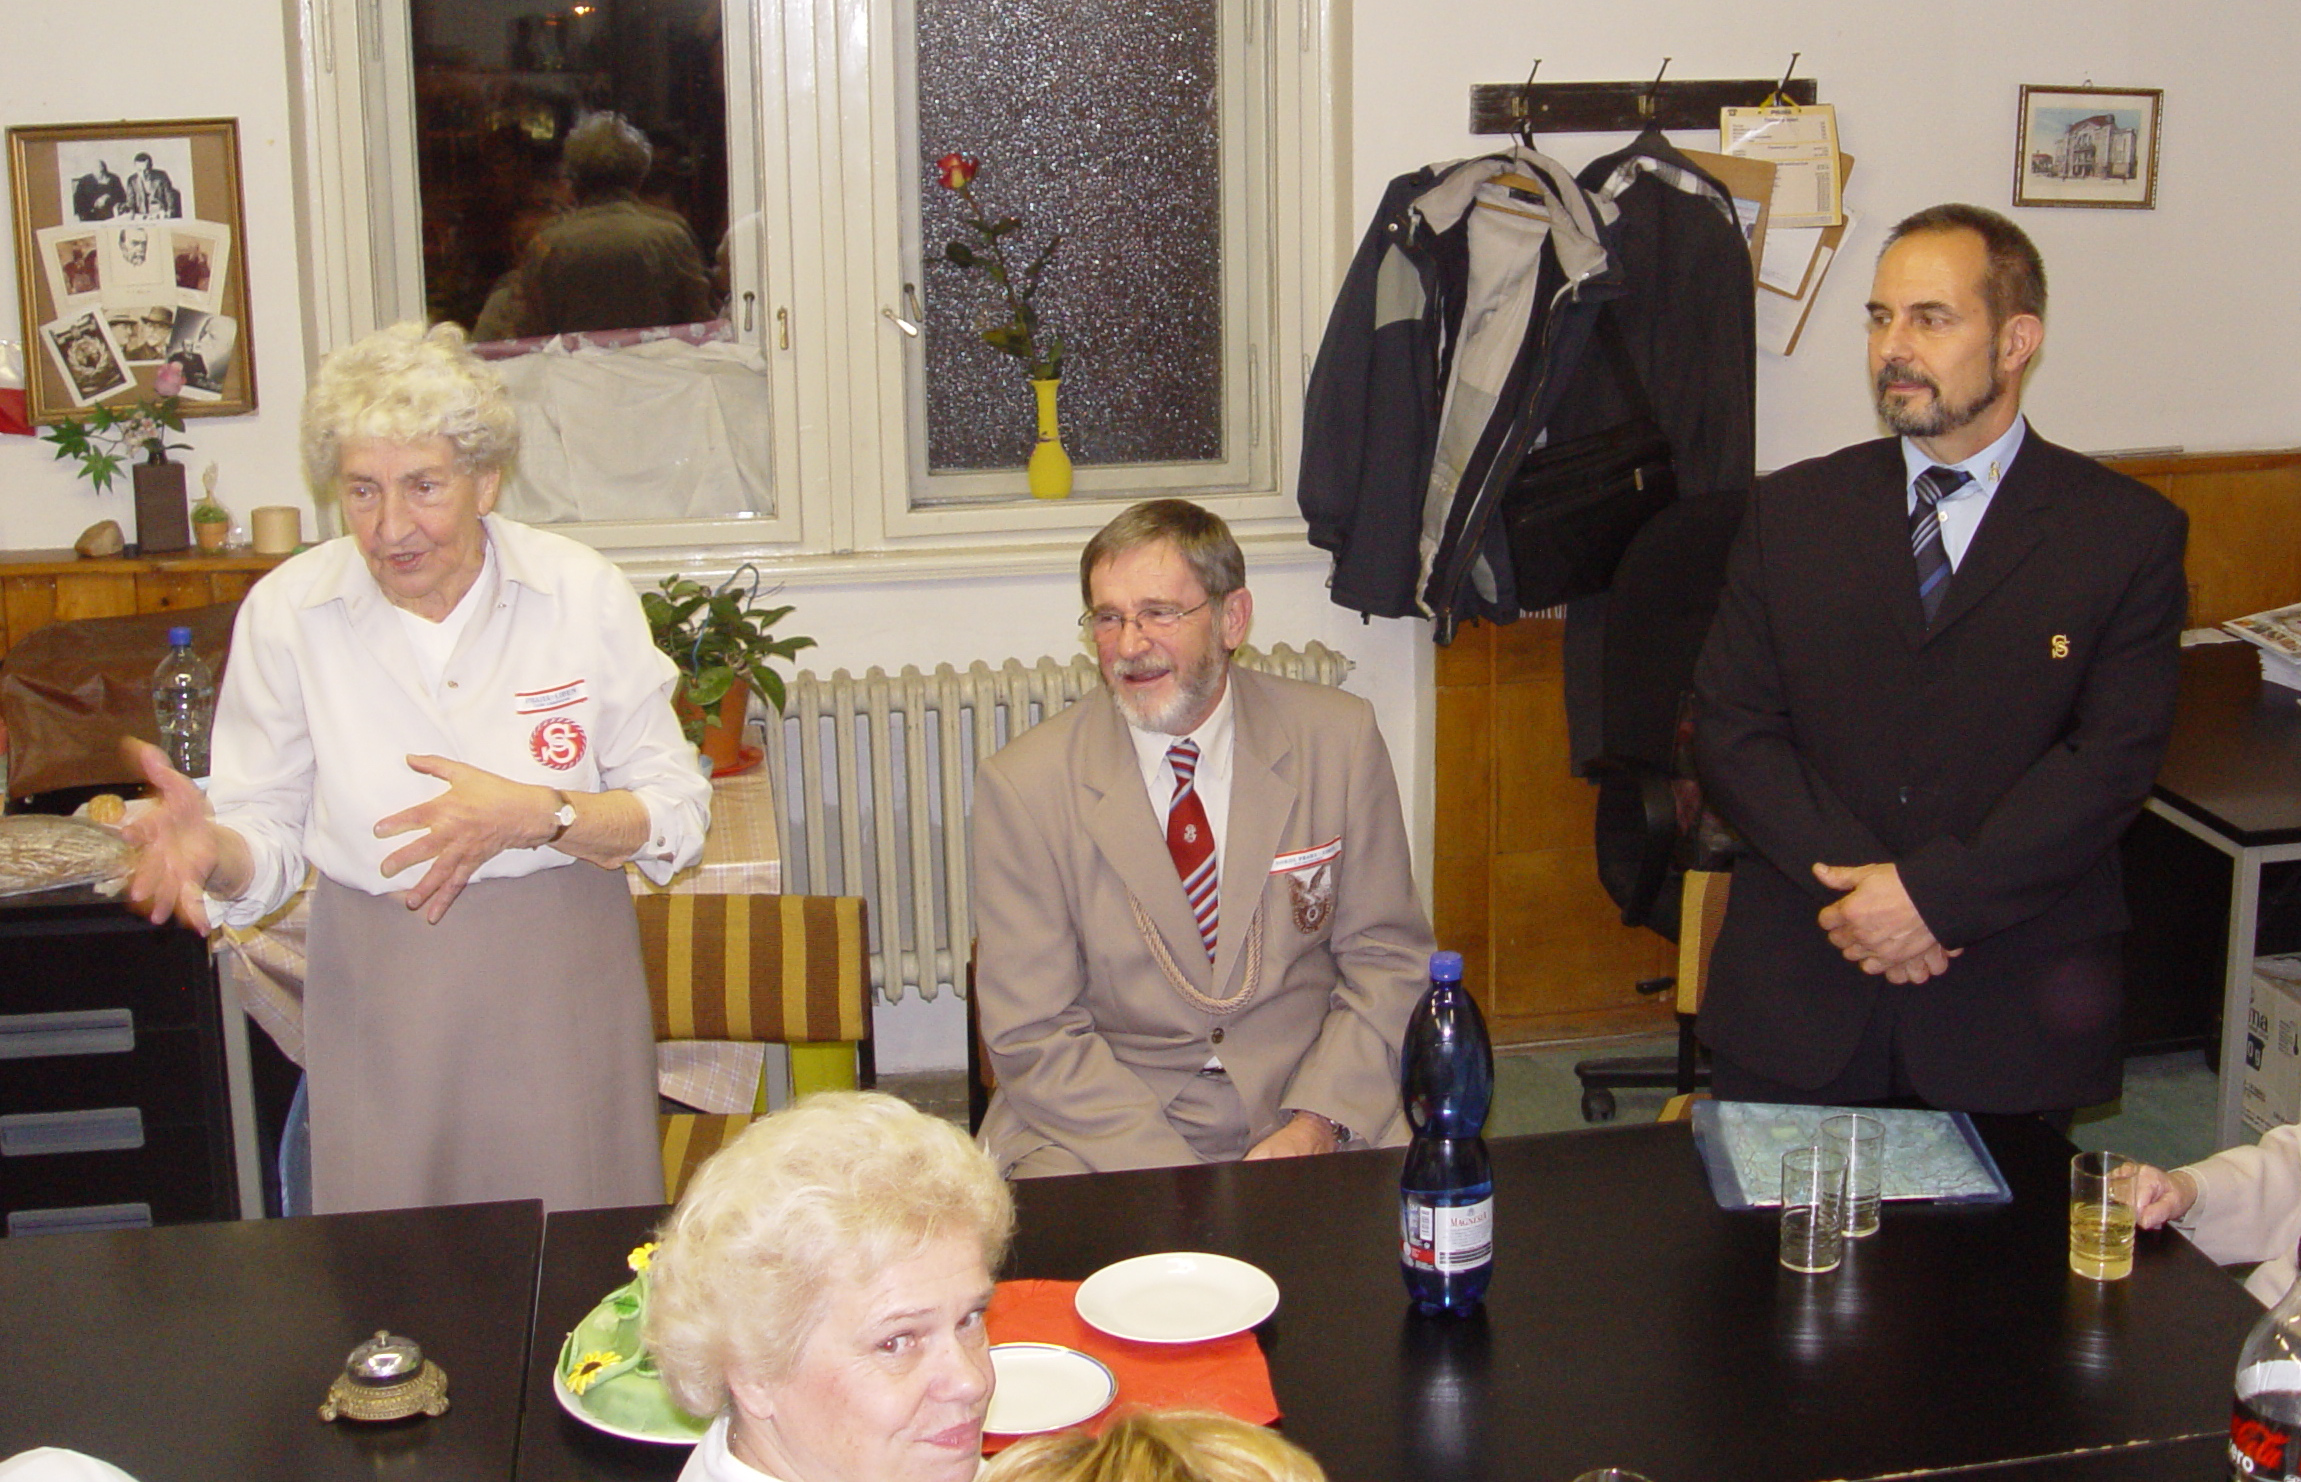
\includegraphics[width=0.9\textwidth]{img/49_debrifink.JPG}
  \caption*{Debrífink po slavnostní akademii k~výročí položení základního
  kamene sokolovny (2009), vlevo: náčelnice ses. Milada Věra Decastellová,
  uprostřed: starosta jednoty br. Jiří Sixta, vpravo náčelník ČOS Miroslav
  Vrána, foto: archiv J. Přecha}
\end{figure*}

K~dalším lidem v~čele jednoty patří jednatel -- ty první se mi dohledat
nepodařilo. Od roku 2004 funkci zastávala Marta Halíková, od roku 2013
je jím Jan Přech. Další důležitou osobou z~hlediska tradice (ale i
součastnosti) je vzdělavatel. Po obnovení Sokola vykonával tuto funkci
František Kodl, po něm Věra Šťastná (1998--2016) a po ní Anna Holanová
(2016--dosud).

Pak tu máme ještě zaměstnance, kteří také spoluvytvářejí obraz naší
jednoty. V~kanceláři to byli v~roli tajemníka či hospodářky: Marta
Halíková, Jiří Sixta, Iva Duchačová, Pavel Pejša a Miluška Malinová.
A~pak už zbývají jen uklízečky a vrátní (ze starších vzpomenu pana
Hatleho, Mifka, z~novějších pana Přibyla a Hofmana).

Tak to je strana jednoty a na straně druhé jsou cvičenci a jejich
(u~těch mladších) rodiče. Pro ty se to vlastně všechno děje. Počet členů se
od roku 1990 do dnešních dnů pohybuje mezi 600 až 1\,000. V~současnosti
je to přibližně 800. Nejsme tedy zrovna malá jednota. Ale snažíme se
držet pospolu. Na JVLS či PVLS se nás občas sejde i okolo stovky, na
akademii bývá i 400 diváků a 250 cvičenců, na posledním sletě (2024)
cvičilo 240 našich členů.

\hfill(\textit{br. Jiří Novák})

\subsection{Provoz jednoty}

{\sloppy Pro provoz jednoty jsou kromě lidí nutné i peníze. Nejprve nakousnu téma
grantů. Nejprve byly určeny pouze pro nákup sportovního vybavení. Tím
jsme však byli po deseti letech přehlceni a už se nevědělo, co rozumného
koupit. Ale třeba skládací stoly a židle se moc hodí na šibřinky a
akademie, na kladinách pilně cvičí žákyně, na zelených čtvercových
žíněnkách zápolí žáci a ve Filipce se vyjímají krásné židle. Dál jsme
investovali do úložných skříní v~nářaďovně obou sálů, do skříní
v~Srncově sále i do skříní na sklo pro šibřinky a další propriety na
chodbě 1. patra. Také nová pódia vyrobená svépomocí dobře slouží pro
kapelu na šibřinkách i jako podložka pod židle v~hledišti akademie.
Naštěstí pak do grantů přibyla položka energie (elektřina, plyn, voda).
Tím jsme měli zase o~trochu snazší život, když vám grant zaplatí
polovinu spotřeby a peníze vám tak zbydou na věci, které z~grantu
zařídit nelze -- třeba opravy a investice. Dalším krokem v~grantech pak
byla právě položka na opravy a údržbu a třeba do grantu magistrátu lze
už několik let dát i položku mzda provozních zaměstnanců. Pravda,
dostaneme tak desetinu mezd, ale i to se počítá a pomůže nám. \par}

S~granty souvisejí finance. Jen taková lehká exkurze do hospodaření
Sokola Libeň. Současný běžný rozpočet je ve výši asi 6,5 milionu\,Kč na
rok. Příjmy jsou cca 2 miliony od nájemců nebytových prostor, cca 2
miliony z~příspěvků, cca 1,75 milionu z~grantů a cca 750 tisíc za nájmy
tělocvičen, dobrovolné dary a jiné nájmy. Výdaje: asi 2,25 milionu padne
na mzdy zaměstnanců, okolo 1,5 milionu padne na energie, 250 tisíc na
daně, 150 tisíc do fondu oprav, 50 tisíc na kancelářské a úklidové
vybavení, 350 tisíc na nákup z~grantů, 750 tisíc na opravy a údržbu;
telefony, internet, EOS, systém badminton 100 tisíc, za známky ČOS 200
tisíc, péče o~cvičitele a členy 200 tisíc, startovné a školení 100
tisíc, drobnější výdaje 200 tisíc, 400 tisíc úspora na příští opravy
sokolovny.

\hfill(\textit{br. Jiří Novák})

\subsection{2004--2006}

Předchozí vydání almanachu se vztahovalo ke 120. výročí jednoty. U~příležitosti tohoto výročí byla zhotovena replika hlavního praporu naší
jednoty, abychom jej mohli ukazovat na všech našich významných akcích.
Více než 100 let starý originál (z~roku 1893) již není ve stavu, ve
kterém by vydržel pravidelné používání. Prapor byl jednotě slavnostně
předán na slavnostní akademii pořádané k~tomuto výročí a jeho kmotrou
byla tehdejší nejstarší členka jednoty, pamětnice prvorepublikové slávy
a dlouholetá cvičitelka a hybatelka dění sestra Marie Kodlová
(1912--2013). 
\begin{wrapfigure}{r}{0.5\textwidth}
  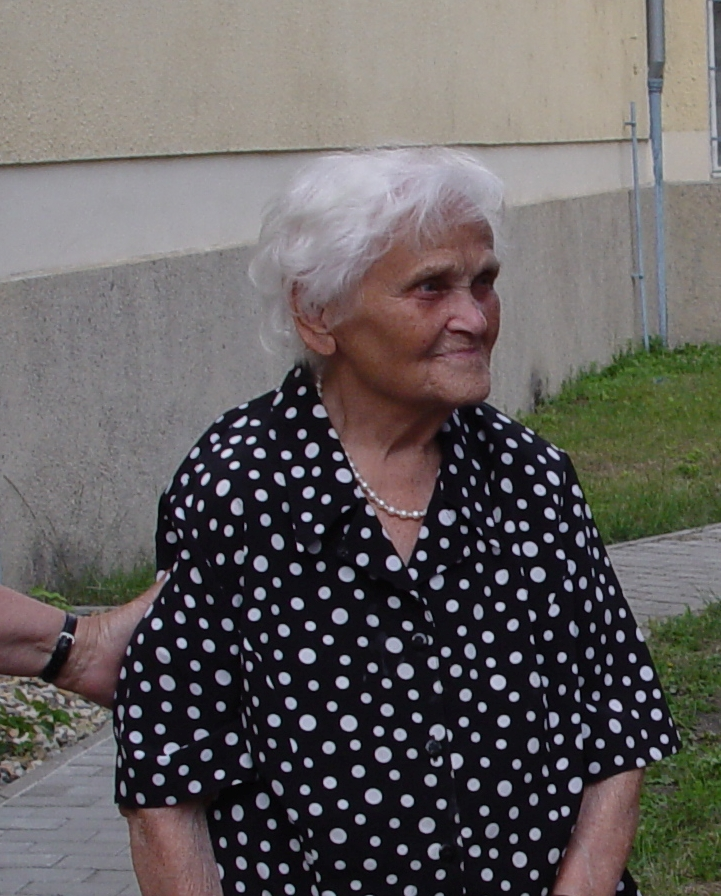
\includegraphics[width=0.9\linewidth]{img/50_manka.jpg}
  \caption*{ses. Marie Kodlová (2008),\\foto: archiv J. Přecha}
\end{wrapfigure}
Tato akademie také představovala završení jakési profesionalizace světel a zvuku, kdy na počátku (v~průběhu 90. let) jsme
svítili klasickým osvětlením sálu, měli jeden mikrofon na kabelu a hudbu
pouštěli z~magnetofonu ve skříni. Na druhou stranu nyní používáme
zvláštní výkonné osvětlení s~barevnými filtry a ovládáním z~režie, režie
se přesunula z~nářaďovny do lodě a hudba se pouští z~CD nebo počítače
přes zvukový mixážní pult. Hlavními hybateli těchto technických změn
byli cvičitelé Vláďa a Pavel Voráčovi s~Martinem Chlumským (Čedokem). Ze
všech akademií od roku 2004 máme též (skoro) profesionální videozáznamy
díky nadšení a práci Standy Voráče (otce Vládi a Pavla). U~příležitosti % TODO chce odstavec?
120. výročí jednoty jsme též rekonstruovali historickou skladbu žáků
z~roku 1920, ke které jsme získali popis a notový zápis hudby pro klavírní
doprovod. Skladbu jsme následně předváděli ještě např. u~příležitosti
80. výročí otevření Tyršova domu na jaře 2005.

Rok 2005 se nesl ve znamení počínajících příprav na XIV. všesokolský
slet. Autorem jedné z~(nejúspěšnějších) skladeb byl také náš cvičitel
Martin Chlumský (pozdější ředitel Ústřední školy ČOS a dnešní starosta
ČOS). Nesla název "Výlet s~Aerobikem" a šlo o~stepaerobikovou skladbu
na hudbu Ivana Mládka. Pro úplnost -- skladba vznikla v~autorské dvojici
s~Janou Beránkovou z~Fakulty tělesné výchovy a sportu Univerzity
Karlovy.

Kromě toho pokračuje postupná oprava sokolovny rekonstrukcí obou velkých
teras (nad lodí s~hrazdami a nad Srncovým sálem) a rekonstrukcí ženských
WC v~1. patře, na které o~rok později navazuje lakování parket v~hlavním
sále.

Umírá další ze zasloužilých libeňských sokolů -- Jindřich Vajkrt.

23.~9. 2005 sletový rok zahájila Sletová štafeta. Jde o~starou tradici,
kterou se rozhodl vzkřísit náš bývalý náčelník Zdeněk Lauschmann a která
spočívala ve štafetovém doručení sletového poselství ukrytého ve
štafetových kolících z~Tyršova domu do sídel všech žup, a to bez použití
motorizovaných dopravním prostředků (s~výjimkou historické tramvaje na
jednom z~úseků v~Praze). Naše jednota byla zodpovědná za úsek vedoucí
z~Tyršova domu do Dřevčic. Po zahajovacím ceremoniálu jsme tedy převzali
kolíky a na lodích je s~transparenty a letáky odvezli po Vltavě do
Libně, kde přenocovaly v~Sokolovně a ráno byly vezeny na kolech do
Dřevčic na první předání. Součet tras všech kolíků, které se za víkend
dostaly do svých cílů, byl úctyhodných 3380 km.

\begin{figure*}[h!]
  \centering 
  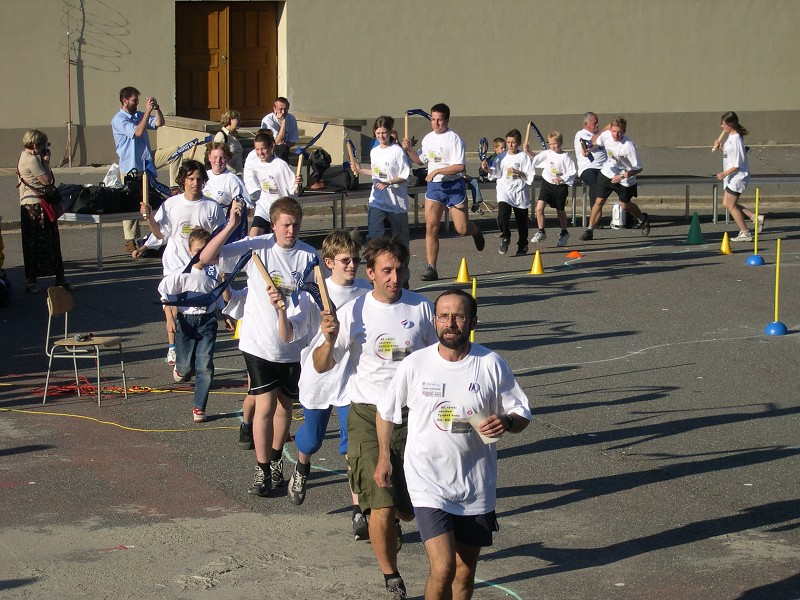
\includegraphics[width=0.9\textwidth]{img/51_stafeta.jpg}
  \caption*{Zahájení Sletové štafety na nádvoří Tyršova domu (2005), první
  běží br. Zdeněk Lauschmann, foto: archiv T.~J. Sokol Libeň}
\end{figure*}

V~roce 2006 se poprvé koná únorové cvičení s~názvem Aerobik Show,
pořádané oddílem aerobiku a našimi cvičiteli Martinem Chlumským
(Čedokem) a Vladislavem Voráčem (Vláďou). Běželo pravidelně až do roku
2016.

\subsection{XIV. všesokolský slet (2006)}

Hlavní událostí roku 2006 byl XIV. všesokoský slet na stadionu E.
Rošického na Strahově. Opět nás čekaly zdlouhavé nácviky, secviky, ale
nakonec to postupně spělo do finále. V~květnu vystupovaly naše skladby
pro dospělé na župním sletu župy Barákovy v~Mělníku, v~červnu pak dětské
skladby na župním sletu na Vinohradech. Sletový týden začal zahájením
sletu se sportovním programem v~Sazka aréně, další den byl sletový
průvod, pak několik dní nácviků a nakonec dvě vystoupení na strahovském
stadionu Evžena Rošického. Z~mužských složek vystoupilo 15 mladších žáků
ve skladbě Karimatky, 10 starších žáků a cvičitelů ve skladbě Výlet
s~aerobikem, jejímž spoluautorem byl náš cvičitel Martin Chlumský (Čedok),
a ve skladbě Chlapáci jsme měli 18 mužů. Celkem měla Libeň na sletu 109
cvičenců v~10 skladbách (včetně společné krokovky "Pozdrav Tobě").
Večerní program byl doprovázen Laserovou show.

\hfill(\textit{br. Jan Přech})

\bigskip

\begin{figure*}[h]
  \centering 
  \includegraphics[width=0.9\textwidth]{img/52_vylet_s_aerobikem.jpg}
  \caption*{V~popředí jeden ze dvou libeňských celků ve skladbě Výlet
  s~aerobikem na oblastním sletu v~Mělníku (2006), foto: archiv T.~J. Sokol
  Libeň}
\end{figure*}

\begin{figure*}[h]
  \centering 
  \includegraphics[width=0.9\textwidth]{img/53_slet_pruvod.JPG}
  \caption*{Libeňské prapory v~cíli sletového průvodu 2006, foto: archiv T.~J. Sokol Libeň}
\end{figure*}

\begin{figure*}[h]
  \centering 
  \includegraphics[width=0.9\textwidth]{img/54_garda.JPG}
  \caption*{Věrná garda z~Libně na XIV. všesokolském sletu (2006), foto:
  archiv T.~J. Sokol Libeň}
\end{figure*}

\begin{figure*}[h]
  \centering 
  \includegraphics[width=0.9\textwidth]{img/55_chalpaci.JPG}
  \caption*{Skladba mužů Chlapáci na sletu 2006, v~popředí lze najít Libeňáky,
  foto: archiv T.~J. Sokol Libeň}
\end{figure*}

\begin{figure*}[h]
  \centering 
  \includegraphics[width=0.9\textwidth]{img/56_karimatky.JPG}
  \caption*{Mladší žáci ze skladby Karimatky na sletu 2006, foto: archiv T.~J.
  Sokol Libeň}
\end{figure*}


\clearpage
\subsection{2006--2012}

Po sletu 2006 začala v~jednotě naplno pracovat generace mladých
cvičitelů přibližně z~roč. 1986--1990 (Martin Seifert, Jan Vorel, Jan
Přech, Jakub Kudroň, Jan Novák, Pavel Lávička, Ája Krásová (roz.
Duchačová), Lucie Vojáčková (roz. Fialová), Barbora Matiášová, Zuzana Burianová (roz. Matiášová) a
další\ldots) a rostla mj. na cvičitelských seminářích v~Libochovicích,
které pořádala Věra Vránová, kdy se naši mladí cvičitelé doopravdy
naučili např. záchranu a dopomoc při sportovní gymnastice. Bohužel
v~únoru 2007 jsme z~této skupiny přišli o~jednoho z~našich nejnadějnějších
cvičitelů a sportovců (soutěžil ve sportovním aerobiku a v~gymnastice)
-- Jana Vorla řečeného "Hnízdo". Hnízdo náhle zemřel 11.~2. 2007
\begin{wrapfigure}{l}{0.5\textwidth}
  \includegraphics[width=0.9\linewidth]{img/57_hnizdo.jpg}
  \caption*{br. Jan Vorel řečený Hnízdo (2008),\\foto: archiv T.~J. Sokol
  Libeň}
\end{wrapfigure}
při epileptickém záchvatu, kdy byl naneštěstí doma sám. Ještě večer před tím
jsme byli spolu plavat v~Tyršově domě na závodu o~Pohár starostů
pražských žup a pamatuju si loučení na mostě přes Vltavu, kdy s~taškou
přes rameno a širokým úsměvem zamával, otočil se a odešel svou
cestou\ldots{} O~několik let později (od roku 2014) jsme na Hnízdovu
počest začali pořádat přátelský závod ve sportovní gymnastice mužů
s~názvem "Memoriál Jana Vorla", kde se mj. scházejí jeho staří kamarádi.
Bohužel nebyl jediný. Odešli též zasloužilí sokolové Vladimír Krotil,
Ludvík Holý a Věra Haufová a také bývalý Jilmák Matouš Vokál.


Sokol, to jsou také hromadná cvičení. Proto se kolem sletů programy
našich akademií plní ukázkami sletových skladeb, ale máme i vlastní
tvorbu. Její ukázkou může být např. skladba dorostenců a mužů "Lavičky"
z~Akademie 2006, kterou jsme následně předváděli ještě na Akademii
Sokola Karlín a na přehlídce pódiových skladeb v~Tyršově domě, kde
skladba získala "cenu za záchranu ohroženého druhu" (\textit{rozuměj
čistě mužského vystoupení}). Léto 2007 s~sebou přineslo také světovou
Gymnaestrádu. Je to nesoutěžní přehlídka všemožného cvičení ze všech
koutů světa a Sokol s~hromadnými skladbami nebo pódiovkami je
pravidelným účastníkem. Z~Libně se Gymnaestrád obvykle účastní 1--2
lidi, kteří mají zájem, a to, že jsou Libeňáci, je veskrze náhoda, ale
rok 2007 a skladba Výlet s~Aerobikem strhla 6člennou výpravu z~Libně,
která si užila 3 vystoupení v~Tyrolském Dornbyrnu a mohla celý týden
čerpat inspiraci z~tance, jiných pódiových skladeb, ale i třeba
sportovní gymnastiky světové úrovně.

S~rokem 2007 ale přicházejí i nové věci. Ústředí České obce sokolské
(ČOS) se začíná vážněji zabývat snahou o~zviditelnění Sokola. První
vlaštovkou je Sokolení -- veřejná akce jednot spojená s~testem
zdatnosti. I~naše jednota se připojila. Stejně jako o~rok později, a to
v~rámci Běhu strmého. Účastníme se i akce Prahy 8 -- Kdo si hraje,
nezlobí -- veletrhu mimoškolních aktivit. Příštích deset let jezdíme do
Bohnic, kde mezi dalšími kroužky nabízíme na prostranství u~kulturního
domu Krakov své aktivity -- máme letáky, cvičení na nářadí, hříčky,
občas lákáme postaveným týpkem do JILMu.

Oddílu JILM si setkáním s~bývalými členy připomněl 25. výročí vzniku.

Tímto rokem začala i naše účast na tradiční akci pražského třížupí --
plaveckém závodu O~pohár starostů pražských žup (založeno 2004), ke
kterému v~roce 2009 přibyl i závod pro děti s~názvem O~minipohár
starostů pražských žup. Každým rokem se najde několik zájemců, kteří za
naši jednotu reprezentují naši župu v~plavání na 50 x 25m.

Sokolovna se toho roku stala i místem svatební oslavy, když se ženil náš
náčelník Jiří Novák. Následovali další cvičitelé a cvičitelky (co si
vzpomínám, tak to byli Vítek Jakoubek, Pavel Voráč, Lucka Fialová (vd.
Vojáčková) a Jan Přibyl).

A~sokolovna neslouží jen svatbám, ale postupně se stala i vyhledávaným
místem pro filmaře. Nejprve se u~nás točily reklamy, castingy
talentových soutěží, z~filmů třeba Lidice, detektivky ČT, Sportovec
roku, opět reklamy, film Svatá atd. Dnes sokolovnu pronajímáme i na
různé oslavy, kulturní technoparty, cizí svatby. Samozřejmostí je
dopolední pronájem tělocvičen pro okolní gymnázia. To vše pomáhá našemu
rozpočtu.

Rok 2008 se nesl ve znamení oslav 90 let moderní české státnosti a naše
akademie přispěla mimo jiného neotřelými živými Obrazy. "Tyršův sen"
znázornil Tyršovu myšlenku kalokagathie na alegoriích antických věd a
umění. Obraz "Kde domov můj" ukázal žehnající kněžnu Libuši. "Křtění
praporu" vycházelo ze stejnojmenné obrazu od Josefa Kočího
zobrazujícího předání prvního sokolského praporu, jehož kmotrou byla
spisovatelka a vlastenka Karolína Světlá. Poslední obraz vzdal hold
československým legionářům, kteří nesou lví podíl na ustavení
Československé republiky a mezi nimiž bylo mnoho sokolů. Dlužno
podotknout, že náš cvičitel Tomáš Novák se v~sokolském kroji M. Tyršovi
velmi podobá, což se nám velice hodilo.

Pavel Voráč uspořádal první volejbalový turnaj pro amatérská mužstva,
který byl pak pořádán asi 10 let, později pod vedením Jiřího Duchače.

Též se domluvilo několik cvičitelů žáků a začali skákat přes švihadlo.
Ne však normální skoky, ale skoky trikové. V~cizině se tomu říká
Ropeskipping. Po dvou letech tréninku se ustavili jako tým Skipping
Boys, který začal jezdit na soutěže. Mohli jste je vidět i v~jedné
televizní talentové soutěži a dodnes skáčou, jezdí na soutěže, a to i na
mistrovství Evropy a mistrovství světa.

Rok 2009 se opět nesl ve znamení slavností, jelikož v~říjnu uplynulo 100
let od položení základního kamene sokolovny. Při této příležitosti byla
vyjmuta časová schránka uložená v~základním kameni a na schůzi výboru
otevřena. Měděná krabice ukrývala písemnosti ze dne jeho položení. Kromě
jiným mezi nimi byly: brožura "Oslava XXV. ročnice tělocvičné jednoty
Sokol v~Praze-VIII.", "Stanovy a řády tělocvičné jednoty Sokol
v~Praze-Libni", brožura "Proč jsem sokolem?", "Cvičitelské Listy",
seznam členů jednoty nebo časopis "Havlíček" ze dne 3.~října 1909.

\begin{figure*}[h]
  \centering 
  \includegraphics[width=0.9\textwidth]{img/58_schranka.JPG}
  \caption*{Obsah časové schránky ze základního kamene sokolovny z~roku 1909
  po otevření dne 4.~března 2009, foto: archiv T.~J. Sokol Libeň}
\end{figure*}

Následně byl základní kámen slavnostně znovu zasazen za přítomnosti
náčelnice ČOS L. Kocmichové, starosty MČ Praha 8 a dalších významných
hostů. Přímo v~hale sokolovny zazněly projevy a zapělo Foerstrovo
komorní pěvecké sdružení. Následně bylo ve Strnadově sále předvedeno
několik ukázek sletových skladeb napříč minulými slety a na závěr zazněl
koncert Hudby Hradní stráže a Policie ČR pod vedením Václava Blahunka.
K~původní časové schránce, která byla do základního kamene vrácena,
přibyla nová dokumentující stav jednoty a také průběh slavnosti po 100
letech od položení základního kamene. Uložili jsme do ní mimo jiné
aktuální číslo časopisu Sokol, sletové pamětní medaile z~let 2000 a
2006, aktuální fotografie cvičitelského sboru a DVD se záznamem
slavnosti. Předpokládáme, že schránky budou znovu otevřeny v~roce 2109.

\begin{figure*}[h]
  \centering 
  \includegraphics[width=0.9\textwidth]{img/59_schranka_2.jpg}
  \caption*{Písemnosti z~časové schránky ze základního kamene sokolovny z~roku
  1909, foto: archiv T.~J. Sokol Libeň}
\end{figure*}

\begin{figure*}[h]
  \centering
   \includegraphics[width=0.7\textwidth]{img/60_zakladni_kamen_jirkan.jpg}
  \caption*{Náčelník br. Jiří Novák znovu ukládá časové schránky do základního
  kamene sokolovny (2009), foto: archiv T.~J. Sokol Libeň}
\end{figure*}

Tento rok se také koná první Den otevřených dveří libeňské sokolovny.
Jedná se spíše o~veřejnost, která je provázena po budově. Až do roku
2017 se poté tato akce pořádá v~rámci Dní evropského kulturního
dědictví. Od roku 2018 pak jako Noc sokoloven, kdy je program více
zaměřen na naše členy a méně na veřejnost. V~roce 2022 se připojujeme
k~akci Open houses.

V~roce 2011 se podařilo zrekonstruovat kotelnu sokolovny, respektive
postavit zcela novou. V~původní kotelně zůstala pouze část technologie a
čtveřice starých plynových kotlů byla demontována a nahrazena trojicí
nových kondenzačních plynových kotlů umístěných spolu s~další
technologií v~bývalé dílně v~rohu sokolovny za ženskými šatnami. Hlavní
zásluha na realizaci patří tehdejšímu starostovi br. Sixtovi. Na podzim
2011 se znovu konala Sletová štafeta, tentokrát s~poselstvím neseným ze
sídel žup do Tyršova domu a rozběhly se přípravy XV. všesokolského sletu
2012. My jsme poselství vezli z~Dřevčic do Tyršova domu, z~Libně na
lodích.

\clearpage
\subsection{XV. všesokolský slet (2012)} se konal na stadionu pražské Slavie
v~Edenu, jelikož Strahovský stadion E. Rošického dospěl do havarijního
stavu (\textit{ve kterém je dosud, pozn. ed.}). Z~Libně se zúčastnilo 102
členů. Za zmínku stojí čistě mužský celek ve skladbě Nebe nad hlavou.
Skladba využívala triková švihadla, a ač byla původně koncipovaná jako
koedukovaná, nakonec vedení sletu rozhodlo, že "chlapi přece přes
švihadlo neskáčou" a skladba bude ženská. Nicméně v~tu dobu už byl
v~Libni složen mimo jiné i kompletní mužský celek, kluci pod vedením Honzy
"Sumce" Dostála měli podporu autorky skladby Jany Beránkové a účast si
vzít nenechali.

\begin{figure*}[p]
  \centering 
  \includegraphics[width=0.9\textwidth]{img/61_muzi_slet_12.JPG}
  \caption*{Muži z~Libně po generálce večerního programu XV. všesokolského
  sletu 2012, foto: archiv T.~J. Sokol Libeň}
\end{figure*}

\begin{figure*}[p]
  \centering 
  \includegraphics[width=0.9\textwidth]{img/62_rd_duchove.JPG}
  \caption*{Rodiče a děti a mladší žactvo z~Libně cvičící ve společné skladbě
  Ať žijí duchové na XV. všesokolském sletu 2012, foto: archiv T.~J. Sokol Libeň}
\end{figure*}

Rokem 2012 začíná období našeho většího zapojení do různých akcí Prahy
8. Tentokrát to bylo zapojení do vzpomínkového aktu na Kobyliské
střelnici, kde se připomínalo 70. výročí akce Anthropoid (atentát na R.
Heydricha). Nacvičili jsme část sletové skladby mužů z~roku 1938 --
Přísaha republice a také předvedli přeskoky na dobovém nářadí.

\clearpage

\subsection{2012--2018}

Po náhlém složení funkce starosty br. Sixtou (br. Sixta se již nenechal
přesvědčit k~dalšímu pokračování ve funkci starosty před valnou hromadou
2013, ale neexistoval záložní plán) nebyl nikdo ze členů na převzetí
starostovské role připraven, a tak se starší cvičitelský sbor a
pokračující část výboru shodly, že bude nutné oslovit někoho zvenku.
Volba nakonec padla na br. Aleše Müllera ze Sokola Malešice a ukázala se
být vynikající. Aleš byl sokol srdcem i duší a současně byl účetní a
schopný manažer, který přijal poslání pomoci nám, aby libeňská jednota
mohla dále fungovat tak, jak byla zvyklá. Lidsky byl Aleš nesmírně
laskavý a vždy měl čas každého vyslechnout a následně se na věc podívat
s~odstupem a zkušeností a poradit nebo obrousit hrany svářících se
stran, ale současně uměl i říci poslední slovo. Díky tomu také velmi
hladce do jednoty, se kterou předtím neměl nic společného, zapadl a
požíval zaslouženého respektu. Aleš se také stal moderátorem debaty
o~budoucnosti. V~rámci cvičitelského výjezdu do Dobřichovic, kde jsme se
pokusili formulovat směry, kam se ubírat v~horizontu delším, než je
příští slet, a pod Alešovým vedením byly zahájeny přípravy velkých
projektů, jako je rekonstrukce dvora a šaten. Dá se také říci, že Aleš
naši novou generaci členů výboru vedení jednoty vlastně naučil. Bohužel
jak náhle jsme Aleše získali, tak náhle jsme ho 27.~2. 2019 ztratili.
Nečekaně zemřel na komplikace spojené s~onemocněním, kterým dlouhodobě
trpěl, ve věku 59 let.

\begin{figure*}[h]
  \centering 
  \includegraphics[width=0.9\textwidth]{img/63_ales.jpg}
  \caption*{Starosta jednoty br. Aleš Müller předává spolu s~náčelnicí Ájou
  Krásovou (uprostřed) a místonáčelnicí Danou Cejpkovou (vpravo) hlavní
  cenu v~tombole na \mbox{Šibřinkách} 2018, foto: archiv T.~J. Sokol Libeň}
\end{figure*}

V~tuto chvíli však jednota již měla nového náčelníka br. Josefa
"Pepištu" Kubištu a br. Jiří "Jirkan" Novák se sice těšil na odchod do
emeritní pozice (\textit{funkci náčelníka zastával od roku 1994 celých 25
let}), ale konstatoval, že starosty by měli dělat starší členové, kteří
už mají odrostlé děti a usazenou kariéru, a že tuto definici teď
naplňuje a funkce starosty jednoty se ujal.

Od roku 2013 přibývá do repertoáru našich akcí novinka pod taktovkou
cvičitele Víta Jakoubka s~názvem Se Sokolem do divadla, kdy se začala
navštěvovat různá divadelní představení. Tato milá nabídka byla
přerušena až v~roce 2020 covidem. V~roce 2023 ji obnovil Míla Doupal.

V~témže roce 2013 postihla Libeň další povodeň. Praha sice byla díky
protipovodňovým zábranám uchráněna, Libni však uškodila. Byla zavřena
protipovodňová vrata u~ústí Rokytky do Vltavy u~louky u~studánky a
Rokytka tak tekla do bývalých libeňských doků, avšak čerpadla, která
měla dostat vodu z~doků do Vltavy, neměla dostatečný výkon a Rokytka se
tak opět vylila z~břehů. Voda byla až u~divadla pod Palmovkou, zaplavila
Voctářovu ulici a napáchala tak velké škody. Sokolovna byla zkázy
ušetřena, jen asi týden nešel proud.

Pod vedením cvičitelů Jana Dostála a Františka Juhásze bylo přistoupeno
k~rekonstrukci posilovny. Nová podlahy, výmalba, zrcadla, obměna
strojového parku.

Také proběhlo promítání fotografií cvičitele Vítka Jakoubka, který půl
roku prožil v~Jižním Súdánu jako lékař v~místní nemocnici.

V~roce 2013 ve 101 letech umírá zasloužilá sokolka Marie Kodlová a 1.~1.
2014 umírá v~požehnaném věku 94 let čestná náčelnice Milada Věra
Decastellová, poslední z~předválečných a těsně poválečných činovníků.

V~březnu 2014 tohoto roku se účastníme (kroje, prapor) vzpomínkové akce
u~sochy Jana Podlipného, což byl starosta Prahy (1897), starosta ČOS
(1889) a zasloužil se o~připojení Libně ku Praze. Na jaře se též
v~sokolovně koná koncert Hudby Hradní stráže v~rámci akce Prahy 8 -- 100
let od narození B. Hrabala.

V~tomto roce je též ve spolupráci s~novým nájemcem Apla zhotoveno nové
doskočiště a je vybudováno nové tartanové rozběžiště a v~září byl
spuštěn elektronický systém matriky a placení příspěvků, jehož jedním
z~autorů byl náš cvičitel Jan Slifka. Systém úspěšně fungoval až do konce
roku 2022, aby byl od ledna 2023 nahrazen zakoupeným a mnohem
dokonalejším systémem EOS.

Cvičitel Josef Kubišta obnovuje cvičení mužů. Muži pravidelně stále
cvičí a stali se jedním z~důležitých hybatelů našeho dění. Letos na
akademii představí nový prapor mužů, který nechali vyrobit k~10. výročí
obnovení cvičení mužů.

Ve spolupráci s~odborníkem na odboj za II. světové války Jiřím Padevětem
jsme se zúčastnili vzniku a odhalení pamětní desky našeho bývalého
náčelníka Bohuslava Strnada, který zahynul pro účast v~odboji. Zde se
sluší připomenout naše krojovaná účast (občas i s~jednotovým praporem)
na akcích připomínající slavnou minulost Sokola a národa -- hrob T. G.
Masaryka v~Lánech, připomínka konce II. světové války, říjnové oslavy
vzniku Československa, účast na Památném dni sokolstva, účast na
oslavách 17.~listopadu a další akce. Postupem doby iniciovala ČOS výcvik
sokolů u~Hradní stráže a vznik tzv. Sokolské stráže pod vedením bratrů
M. Mandy a L. Křemena. V~ní máme několik členů.

V~roce 2015 proběhl první ročník soutěže ČOS v~darování krve s~názvem
Sokolská kapka krve, jejímž iniciátorem byl náš cvičitel Vít Jakoubek.
Naše jednota samozřejmě patří mezi pravidelné účastníky (viz zvláštní
článek).

Kupujeme airtrack a cvičitelé František Juhász a Jáchym Kaplan stáli za
zrodem zkušebny pro kapely v~chodbě archivu ve 3. patře sokolovny.

{\sloppy S~ohledem na časté krádeže v~šatnách v~předchozích letech bylo
přistoupeno k~celkové obnově klíčnictví. Dveře do šaten byly vybaveny
samozamykacími zámky s~koulí na dveřích z~vnějších stran a s~odemykáním
na čip. Stejné zámky byly dány i na dveře z~galerie na zadní schodiště,
aby se nikdo do šaten nemohl dostat do šaten ani touto cestou a byl
zaveden systém generálního klíče s~různými úrovněmi oprávnění. \par}

V~roce 2017 byla na popud Vítka Jakoubka byla zhotovena nová pamětní
deska, která připomíná jména sokolů, kteří v~naší sokolovně udrželi
myšlenku sokolství i v~dobách nesvobody v~letech 1948--1989.
Deska je umístěna na chodbě 1. patra sokolovny.

V~rámci zviditelňování Sokola pro veřejnost jsme pro ČOS vystupovali
(např. Skipping Boys) v~doprovodném programu veletrhů For kids
v~Letňanech v~letech 2016 a 2017 a připravili jsme si další vystoupení pro
Prahu 8 v~rámci oslav 120 let otevření tramvajové tratě Praha -- Karlín
-- Libeň. Předvedli jsme sletovou skladbu mužů ze sletu 1912 a náš
prapor z~roku 1893, který opravdu ty tramvaje mohl v~roce 1896 vítat.
Vystoupili též Skipping Boys. Zemřela naše vzdělavatelka Věra Šťastná.

V~roce 2017 byl ustaven oddíl šplhu, který se postupem doby stal jedním
ze tří nejlepších v~České republice. Řada jeho členů plní limit 10
vteřin ve šplhu ze sedu bez přírazu na osmimetrovém laně, a může se tak
účastnit mistrovství republiky. Postupem času začali šplhat i dorostenci
a nakonec zlákali i ženy. Třeba během posledního sletu vystupovali
v~programu Sokol gala.

Pro naše cvičitele jsme také připravili speciální celodenní školení
gymnastiky od špičkových lektorů. Prostě jsme se zase chtěli posunout
o~kousek výš v~našich znalostech a dovednostech. V~sokolovně se konala
výstava k~výročí operace Anthropoid.

Uplynulo dalších 6 let a v~září 2017 je tu opět start sletového roku
Sletovou štafetou. Tentokráte se jedná o~akce župní. Jedna možnost byla
vystoupení na akci v~hostivařské sokolovně a následně přejezd
historickou tramvají do Tyršova domu. Druhá možnost pak klasicky kánoí
z~Libně do Čertovky a Tyršova domu.

V~roce 2018 probíhala rekonstrukce Zenklovy ulice. V~rámci toho byl
změněn tvar chodníku před sokolovnou, který byl následně hezky
vydlážděn. Před sokolovnou vznikla i stanice tramvaje s~názvem Libeňský
zámek. My využili situace a stejným způsobem jsme si od realizační firmy
nechali za asi 140\,000\,Kč vydláždit náš pozemek před vrátky na jižní
straně sokolovny. Z~grantů jsme koupili přenosnou hrazdu do sálu a také
nová mužská bradla.

\subsection{XVI. všesokolský slet (2018)}

Ač se to nezdá, další slet je před námi, nacvičujeme, secvičujeme se
různě po Praze s~dalšími celky. Na podzimní akademii jsme předvedli
několik krátkých ukázek sletových skladeb (pro nalákání dalších
cvičenců). No a už je tu květen a s~ním župní slet v~Brandýse nad Labem.

A~pak 1.~července sletový průvod -- z~Libně se účastnilo asi 85
cvičenců, následně Sokol gala (vystupoval Patrik Valut z~oddílu šplhu na
11metrovém laně a kluci ze Skipping Boys), úmorné secviky a nakonec
vytoužená vystoupení. Libeňáci cvičili v~9 z~11 skladeb. Bylo nás celkem
146 (92 dětí a 54 dospělých) a cvičili jsme na 166 značkách (někdo byl
ve více skladbách). Ve skladbě pro mladší žáky "Děti, to je věc"
cvičilo 16 kluků, ve společné skladbě pro starší žactvo jsme měli 18
kluků a 18 holek, do společné československé skladby "Spolu" se vydalo
12 mužů a 2 ještě cvičili ve skladbě Věrné gardy "Princezna
republika". Slet totiž korespondoval se 100. výročím vzniku
Československa.

\begin{figure*}[hp]
  \centering 
  \includegraphics[width=0.9\textwidth]{img/64_siluety.JPG}
  \caption*{XVI. všesokolský slet 2018, skladba dorostenek a mladších žen
  Siluety, foto: archiv T.~J. Sokol Libeň}
\end{figure*}

\begin{figure*}[hp]
  \centering 
  \includegraphics[width=0.9\textwidth]{img/65_zenobrani.JPG}
  \caption*{XVI. všesokolský slet 2018, skladba žen Ženobraní, foto: archiv T.
  J. Sokol Libeň}
\end{figure*}

No a hned další den po zakončovacím sletovém táboráku se jelo stavět
tábor. Ani o~prázdninách Sokol nespí. 8 týdnů táborů (JILM, Káňata,
bývalí členové JILMu, Veverky) a je tu pondělí 2.~září a začíná další
cvičební rok. Běh strmý, Noc sokoloven, PVLS, podzimní brigáda,
akademie, Mikuláš, Loutkáři, Silvestr cvičitelů, šibřinky, Memoriál Jana
Vorla, nominační závody žáků, jarní brigáda, JVLS, Závody všestrannosti,
Dětský den, Zakončovací táborák, tábory. A~tak stále dokola. Ale děti se
mění, rostou, vybírají si jiné akce než před rokem. A~hlavně stále
přicházejí nové tváře. A~není jich málo. Vždyť jen v~oddílech mladších a
starších žáků je asi 40 nových duší. A~to nemluvím o~těch nejmenších
z~oddílů Rodiče a děti a Předškoláci, kde ročně přibude i 100 nových
cvičenců.

Umírá jedna z~našich průkopnic cvičení rodičů s~dětmi, bývalá cvičitelka
Anička Kavinová.

\afterpage{\clearpage}

\subsection{2019--2024}

Dění v~Libni po roce 2018 je vlastně současnost a o~té se špatně píše do
almanachů, protože chybí patřičný časový odstup. Jistě lze říci, že
dochází k~další významné generační obměně aktivního cvičitelského sboru
(pokud pomineme nestory jako bratři Novákovi), neb silná generace
zmíněná po roce 2006 zakládá rodiny nebo postupně odpadá ve víru práce a
nekonečných možností, které dnešní svět nabízí. Rozvíjejí se také nové
oddíly. O~obojím pojednává současný náčelník br. Kubišta ve svém
příspěvku.

V~roce 2019 přibývá další tradiční akce. Památný den sokolstva. Jde
o~připomenutí obětí II. světové války, kdy 8.~10. 1941 byl Sokol zakázán a
více než 1\,500 vedoucích činovníků zatčeno a postupně umučeno. V~roce
2019 je také po třech letech Anna Holanová oficiálně zvolena na valné
hromadě jednoty vzdělavatelkou a dochází ke vzkříšení vzdělavatelského
odboru. Kromě běžných akcí je činnost rozšířena i o~různé vzdělavatelské
vycházky. Postupně se opět začíná psát kronika jednoty. Vzniká oddíl
přetahu lanem a také začíná tradice Tančíren -- setkání cvičitelů a
jejich hostů na tanečních večerech.

{\sloppy Kromě toho, že v~únoru nečekaně zemřel náš starosta Aleš Müller, také
v~březnu podlehla cystické fibróze mladá cvičitelka a Jilmačka Ester
Lammelová.\par}

Do chodu jednoty, podobně jako do chodu celé společnosti silně zasáhla
pandemie nemoci covid-19. Snad poprvé od války bylo nutné v~naší
sokolovně přerušit na dlouhé týdny cvičení. Dva měsíce od března do
května se nesmělo vůbec cvičit, pak s~omezením, a na podzim totéž od
října do prosince. Před Vánoci 14 dní cvičíme a od 18.~prosince 2020 do
10.~května 2021 je vše úplně uzavřeno. Chvála Bohu úmrtí na covid-19 se
naší jednotě vyhnula. Volný čas jsme pod vedením náčelníka br. Kubišty
využili k~zahájení některých dlouho odkládaných rekonstrukcí, které šlo
dělat po jednom nebo jen v~malé skupině při dodržení proticovidových
pravidel. Rekonstrukce se tak dočkala kromě jiného sborovna nebo
místnost v~přízemí, která byla připojena k~pronajatým prostorám školky
Nautis. Navazuje i rekonstrukce kanceláře jednoty. Po letech snažení a
jednání zahájeného starostou br. Müllerem také dostáváme stavební
povolení na rekonstrukci dvora a na rekonstrukci šaten.

Po odeznění pandemie se členové naší jednoty (15 osob, mužů i žen)
zúčastnili kromě jiného akce SokolGym, kde účinkovali v~hromadné skladbě
Odhodlaní. Skladba v~choreografii Heleny Peerové a na epickou hudbu Two
Steps from Hell patřila k~tomu nejlepšímu, co bylo v~Plzni, Brně a
Pardubicích předvedeno, ale více než dvouleté roztažení původně
jednosezónního projektu bylo dosti bolestivé. Nácvik vedla Zuzana
Dočekalová.

\begin{figure*}[t]
  \centering 
  \includegraphics[width=0.9\textwidth]{img/66_odhodlani.jpg}
  \caption*{Vystoupení skladby Odhodlaní na SokolGym 2022 v~Plzni, foto:
  archiv J. Přecha}
\end{figure*}

V~létě 2022 se začíná stavět na dvoře u~kostela podzemní místnost (nová
loděnice), která je dokončena na jaře 2023. Díky chybám (ne na naší
straně) a úřednímu šimlovi dosud bojujeme s~kolaudací. Se stavbou
místnosti byla postavena i nová opěrná zídka směrem ke kostelu, opravilo
odvodnění kostela a také rozebrána a znovu postavena část opěrné zdi
směrem ke gymnáziu, která hrozila zřícením.

\begin{figure*}[hp]
  \centering 
  \includegraphics[width=0.9\textwidth]{img/67_zzz.JPG}
  \caption*{Libeňští organizátoři a závodníci (v~přední řadě) na republikovém
  přeboru ČOS v~Zálesáckém závodu zdatnosti, Machův mlýn 2023, foto: J.
  Novák}
\end{figure*}

\begin{figure*}[hp]
  \centering 
  \includegraphics[width=0.9\textwidth]{img/68_vh_22.jpg}
  \caption*{Cvičitelky, cvičitelé a činovníci T.~J. Sokol Libeň přítomní na
  valné hromadě 2022, foto: archiv T.~J. Sokol Libeň}
\end{figure*}


Rok 2023 byl přelomový ve dvou věcech: jednak se naše jednota se poprvé
odhodlala k~uspořádání republikového přeboru ČOS v~Zálesáckém závodu
zdatnosti (kterého se naše turistické oddíly pravidelně účastní po
většinu jeho historie). Ředitelem závodu a hlavním koordinátorem celé
akce byla moje maličkost (Jan Přech), ale bez podpory dalších členů
A-týmu Jirkana, Ledňáčka, Jany Dubské, Pepy Kubišty a Míly Doupala ani
dalších pomocníků by to rozhodně nešlo. Velkou podporou nám byl také 3.
místonáčelník ČOS Honza Nemrava ze Sokola Olomouc -- Nové Sady, který
byl hlavním rozhodčím a také tím, kdo mě hecnul, že "to zvládneme" a
stojí to za to udělat. Přebor konaný na Machově Mlýně (okres Rakovník)
se v~některých bodech (třeba autobus pro svážení lidí z~Rakovníka na
poslední chvíli) vyznačoval notnou dávkou štěstí, ale vše se podařilo a
ohlasy všech 196 účastníků byly pochvalné.

Druhou přelomovou událostí, ve které jsme také měli notnou dávku štěstí,
byla kompletní rekonstrukce šaten v~hodnotě přes 10,5 milionu\,Kč.
Jelikož se nám díky grantům a dobrému hospodaření podařilo našetřit
slušné peníze, začali jsme pomýšlet na velké rekonstrukce sokolovny a
okolí. Nechali jsme tedy připravit studii a projekt rekonstrukce dvora
sokolovny zahrnující stavbu nové loděnice a druhý na kompletní
rekonstrukci šaten (zahrnující vybourání klecí ze 70. let a nové
sociální zařízení). Během roku 2021 se povedlo získat stavební povolení
a v~roce 2022 jsme tedy poprvé žádali o~investiční grant z~Magistrátu
hl. m. Prahy. Jelikož žádost nebyla úspěšná, pustili jsme se do
rekonstrukce dvora, kde prvním krokem byla právě nová loděnice (2,5 mil.
Kč; ta mimochodem do této chvíle -- na rozdíl od šaten -- není
zkolaudovaná; víc o~tomto příběhu ve Zprávách jednoty z~poslední doby).
V~roce 2023 jsme zažádali znovu, ale z~důvodu problematického skládání
nové koalice po volbách se vyhlášení výsledků vleklo až do června a až
někdy v~květnu jsme dostali avízo, že jsme dostali 6 milionů\,Kč.
Následovalo tedy bleskové vypsání veřejné soutěže, vyřezání klecí ze 70.
let a po doběhnutí všech lhůt jsme staveniště předávali 17.~července a
ještě týž den začali dělníci pracovat s~tím, že má být hotovo do 30.
listopadu. Podmínky grantu totiž požadovaly kolaudaci do konce roku,
následně prodlouženou do konce března 2024, ale fyzicky hotovo muselo
být do konce roku. Termín byl šibeniční, ale br. starosta při
rozhodování v~květnu prohlásil, že si myslí, že by to mělo vyjít, a
vyšlo. Nové šatny, otevřené k~provozu 19.~2. 2024, respektují secesního
ducha sokolovny, ale konečně patří do 21. století.

\begin{figure*}[hp]
  \centering 
  \includegraphics[width=0.9\textwidth]{img/69_satny_stare.JPG}
  \caption*{Šatny před rekonstrukcí (2023), foto: archiv T.~J. Sokol Libeň}
\end{figure*}

\begin{figure*}[hp]
  \centering 
  \includegraphics[width=0.9\textwidth]{img/70_satny_nove.JPG}
  \caption*{Zrekonstruované šatny (2024), foto: archiv T.~J. Sokol Libeň}
\end{figure*}

V~roce 2023 se také začal odvíjet příběh oddílu Akrojógy pod vedením
sester Kolářových a zemřela naše dlouholetá hospodářka a jednatelka
Marta Halíková.

\clearpage
\subsection{XVII. všesokolský slet (2024)}
A~XVII. všesokolský slet v~roce 2024? To je současnost. Letos se nás
z~Libně pro slet rozhodlo nebývalé množství. Doteď nejvíce nás bylo na
posledním sletu v~roce 2018, a to 146. Letos nás bylo skoro o~sto více,
tedy přesně 240. Obsadili jsme 274 značek a cvičili v~10 z~12 skladeb.
Cvičilo 137 dětí a 103 dospělých. Z~mužských složek cvičilo 22 mladších
žáků ve skladbě "Sokolhraní", 24 starších žáků a cvičitelů cvičilo
skladbu staršího žactva "Fitness" (+18 holek), 36 mužů se předvedlo ve
skladbě "Před kamerou". Naše ženy nechyběly ve skladbách "V rytmu
srdce", "Leporelo" a "Babí léto", mladší žákyně se ukázaly ve
skladbě "Čarodějky" a nechyběli ani rodiče a děti ("Čmeláčci") a
předškolní děti ("Mravenci"). Velmi symbolická byla skladba seniorů
"Jdi za štěstím", do které až v~jejím průběhu nastoupili v~odlišných
úborech nejstarší členové sokolské Věrné gardy -- poslední pamětníci
sletů 1938 a 1948. Jak zpíval Karel Gott v~hudebním doprovodu: "Čas dál si běží svůj maraton\ldots".

\begin{figure*}[p]
  \centering 
  \includegraphics[width=0.9\textwidth]{img/71_sokolhrani.jpg}
  \caption*{Skladba Sokolhraní mladšího žactva na XVII. všesokolském sletu
  (2024) předvedená před vyprodaným stadionem v~Edenu, foto: archiv T.~J.
  Sokol Libeň}
\end{figure*}

\begin{figure*}[p]
  \centering 
  \includegraphics[width=0.9\textwidth]{img/72_rytmus_srdce.jpg}
  \caption*{Skladba žen V~rytmu srdce na XVII. všesokolském sletu (2024),
  v~popředí dva celky Sokola Libeň, foto: archiv T.~J. Sokol Libeň}
\end{figure*}

\section{Věra Decastellová -- jeden sokolský život na pozadí dějin 20.
století}

\begin{center}
  \textit{Řeč pronesená na pohřbu čestné náčelnice naší jednoty ses. Věry
  Decastellové (leden~2014), autorem řeči byl br. Vít Jakoubek}
\end{center}

\noindent
Vážené sestry, vážení bratři, milí přátelé Věry Decastellové, rád bych
vás jménem rodiny a též jménem sokolské jednoty v~Praze-Libni přivítal
na rozloučení s~naší čestnou náčelnicí.

Myslím, že nemá význam ji titulovat jinak. Posledních více než 20 let
byla pro nás libeňské sokoly sice také Věrou, ale velmi často se
stávalo, že jsme o~ní mluvili pouze jako o~"náčelnici". A~nemohli jsme
ani jinak -- Věra zastávala tuto funkci od obnovení naší jednoty v~roce
1990 do roku 2012, kdy se stala čestnou náčelnicí jednoty. Věra byla
sokol tělem i duší a svou jednotou doslova žila.

Věra se narodila v~roce 1919 rodičům, kteří se poznali v~Sokole a
v~sokolském duchu vychovávali i své děti. Věřina maminka také nějakou dobu
zastávala funkci náčelnice Sokola Libeň. Rodina žila po celou dobu,
kromě válečných let, v~Libni a s~Libní jsou neodlučně spjaty všechny
Věřiny životní události -- a že jich nebylo málo.

Od září roku 1925 začala Věra chodit do cvičení v~Sokole, a jak rostla,
postupně se zapojovala více a více do činnosti v~jednotě. Na sletě
poprvé cvičila v~roce 1932. S~přibývajícími lety se zapojila též do
cvičitelské činnosti -- věnovala se zejména dorostenkám a cvičitelské
zkoušky složila po slavném sletě v~roce 1938, kde mimo jiné cvičila ve
všech třech skladbách pro ženy. Bohužel, poměrně krátce na to zahalil
zemi stín II. světové války a v~této nelehké době měla Věra možnost
osvědčit to, k~čemu byla v~Sokole vychovávána a vedena: čestnost,
obětavost, vytrvalost a vlastenectví. Věřin bratr, štábní kapitán Josef
Decastello, po začátku okupace odletěl do Francie, kde při vojenské akci
ve svém letadle zahynul. Rodina byla proto nacisty od začátku války
sledována, a ač se Věra, vlastně díky zranění maminky, vyhnula nucenému
nasazení v~Říši, po atentátu na Reinharda Heydricha byla spolu se svou
sestrou a otcem internována v~táboře ve Svatobořicích. Z~jejího
vyprávění víme, co vše tam bylo lze zažít a jak se sama snažila
zpříjemnit pobyt svým blízkým nejen slovem, ale i činy. Propuštění se
dočkala po bezmála dvou letech v~roce 1944.

Po návratu domů na konci války se opět naplno zapojila do činnosti
libeňského Sokola. Po vyklizení sokolovny, kde byl sklad vojenského
materiálu, začalo naplno pravidelné cvičení a též nácvik na XI.
všesokolský slet. Věra cvičila ve třech ženských a dvou dorosteneckých
skladbách. Ve třech poválečných letech též vedla letní tábory libeňských
dorostenek.

Na podzim 1948 však Věra musela jednotu po zásahu "akční komise" nuceně
opustit a 20 let do sokolovny nevkročila. Teprve v~roce 1968 se
s~příslibem uvolnění poměrů do jednoty vrátila. Ač nakonec nastoupila
normalizace, Věra spolu s~dalšími přesvědčenými libeňskými sokoly
(\pozned{např. manželé Kodlovi, pozn. ed.}) prohlásila, že se již znovu
vyloučit nenechají a následujících 20 let se tedy
\begin{wrapfigure}{r}{0.5\textwidth}
  \centering 
  \includegraphics[width=0.9\linewidth]{img/73_vera_cedok.JPG}
  \caption*{Náčelnice ses. Milada Věra Decastellová na akademii v~roce 2009,
  foto: archiv T.~J. Sokol Libeň}
\end{wrapfigure}
společně snažili
udržet sokolskou myšlenku v~Libni, jak to šlo. Jsou zde jistě pamětníci,
kteří mohou potvrdit, že úspěšně. Vždyť nebýt jí podobných, nebylo by po
revoluci v~roce 1989 možné tak rychle obnovit libeňské jednotu i činnost
v~ní. V~roce 1990 byla Věra zvolena náčelnicí jednoty, obnovila ženský
cvičitelský sbor a zapojila se též aktivně do příprav XII. všesokolského
sletu. A~to nejen na úrovni jednoty, ale i na úrovni celostátní, kdy
utvořila s~dalšími sestrami stravovací skupinu a připravovala jídlo pro
účastníky mnoha nácvičných srazů.

Na celostátní úrovni byla činná i v~Ústředním cvičitelském sboru žen a
seniorek. Věra se velmi obětavě starala o~archiv naší jednoty a při
významných příležitostech pořádala výstavy a ukazovala mnohdy velmi
cenné historické dokumenty, z~nichž některé osoby na fotografiích mohla
poznat již jen ona sama (\pozned{Věra je spoluautorkou výběru historických
fotografií pro tento almanach, pozn. ed.}). Já sám si z~nedávné doby
vzpomenu například na štos přihlášek sokolů zpět do jednoty z~roku 1968
nebo fotografie z~letních táborů těsně po válce. Velmi aktivně se
zapojovala i do běžného chodu jednoty, a to i v~dobách, kdy jí zdraví
již tolik nesloužilo. Řada z~nás si pamatuje mnohdy velmi ostré diskuze
při výborových schůzích, kdy se Věra nikdy nebála vyslovit i třeba
menšinový názor a v~následné debatě jej tvrdě hájit.

Věra cvičila naposledy na sletě v~roce 2006 ve skladbě \textit{Ta naše
písnička česká}. Byť ne jako cvičenka, ale přesto velmi aktivně se
zúčastnila i posledního, XIV. všeskokolského sletu, kde snad nebyla
akce, kterou by nenavštívila.

Blaho libeňské jednoty měla Věra na mysli až do konce. Loni na jaře, kdy
již neměla síly dojít do sokolovny, jsme s~Věrou natáčeli sérii
rozhovorů, ve kterých nám převyprávěla skoro celý svůj život. Při
rozhovoru krátce před valnou hromadou Věra asi po hodině prohlásila:
"Hele, vypni to -- to můžem dodělat příště. Teď musíme vymyslet, kdo by
mohl být novým starostou." Původní starosta Sokola Libeň (\textit{br.
Sixta}) totiž nečekaně oznámil, že již nebude znovu kandidovat.

Za své zásluhy byla oceněna zlatou medailí ČOS a též navržena na státní
vyznamenání.

Milá Věro, rád bych Ti za nás všechny poděkoval za to, čemu jsi nás
naučila, k~čemu jsi nás vedla a jakým vzorem jsi pro nás všechny byla.
Snad mohu též za nás všechny slíbit, že se Ti budeme snažit vyrovnat a
být Ti důstojnými pokračovateli, abys i nadále mohla mít ze Sokola jen a
jen radost.

 \clearpage
\section{Současná činnost oddílů ženských složek
v~Libni}

\begin{center}
  \textit{Sepsali Iva Duchačová, Lenka Malečková, Josef Maleček a Věra
  Šťastná pro Almanach 2004, doplnil/aktualizoval Jan Přech 2024}
\end{center}

\noindent
V~roce 2024 pracuje cvičitelský sbor žen v~abecedně následujícím
složení:

\bigskip

% \begin{multicols}{2}
  \begin{itemize}[label={},itemindent=-2em,leftmargin=2em,nosep]
  \item Agáta Adámková (žákyně)
  \item Zuzana Burianová (sletová skladba V~rytmu srdce)
  \item Dana Cejpková (rodiče a děti předškolní děti, sletová skladba Mravenci)
  \item Zuzana Dočekalová (předškolní děti, sletová skladba Leporelo)
  \item Tomáš Dragoun (náčelnice, žákyně; \textit{stanovy ČOS nepředepisují, že funkci náčelnice musí zastávat osoba ženského pohlaví, a tak  si ženský cvičitelský sbor pokrokově zvolil cvičitele žákyň br. Dragouna a tituluje ho "náš náčelnice" pozn. ed.})
  \item Jana Dubská (rodiče a děti, žákyně, ženy -- všestrannost, sletová skladba Fitness),
  \item Iva Duchačová (předškolní děti)
  \item Anna Feřtová (předškolní děti, žákyně),
  \item Dáša Francková (předškolní děti, ženy-seniorky, sletová skladba Babí Léto)
  \item Anna Holanová (žákyně)
  \item Evženie Hraničková (emeritní cvičitelka žen-seniorek, t. č. již necvičí)
  \item Zuzana Hrušková (předškolní děti),
  \item Martin Chlumský (ženy -- kondiční cvičení)
  \item Květa Kerhartová (žákyně)
  \item Richard Kloubský (žákyně)
  \item Anna Kolářová (akrojóga)
  \item Markéta Kolářová (akrojóga)
  \item Alena Krásová (ženy -- všestrannost)
  \item Martin Kubů (předškolní děti)
  \item Romana Lorencová Bláhová (ženy -- kondiční cvičení),
  \item Josef Maleček (žákyně -- družstvo sportovní gymnastiky)
  \item Alena Markantová (ženy-seniorky)
  \item Jana Motlová (rodiče a děti, ženy-seniorky)
  \item Věra Nosková (ženy -- kondiční cvičení)
  \item Lenka Nováková (žákyně)
  \item Adéla Přechová (předškolní děti)
  \item Barbora Přechová (sletová skladba V~rytmu srdce)
  \item Eva Šádková (předškolní děti žákyně)
  \item Martina Škochová (sletová skladba Čmeláčci)
  \item Anežka Valutová (žákyně)
  \item Klára Veselá (ženy -- kondiční cvičení)
  \item Lucie Vojáčková (předškolní děti, žákyně, sletová skladba Čarodějky)
  \item Jana Voráčová (žákyně)
  \item Vladislav Voráč (ženy -- kondiční cvičení)
  \end{itemize}
% \end{multicols}
\smallskip
\noindent
\pozned{(sestry, u~kterých je uvedena
pouze sletová skladba, se jinak pravidelnému vedení cvičení nevěnují,
pozn. ed.)}.

\subsection{Rodiče a děti}

Libeňská sokolovna ožívá cvičením oddílu Rodičů a dětí již od
osmdesátých let, a~to nejdříve pod vedením vzorné cvičitelky Aničky
Šmejkalové, později pod vedením cvičitelky Aničky Kavinové. Do cvičení
rodičů a dětí chodí děti již od dvou let. Cvičitelce Anně Kavinové,
která se celý život věnuje tomuto cvičení, prošlo rukama snad několik
generací cvičenců. Už od obnovení Sokola se tady ozývají národní
písničky, kterými svá cvičení doprovází. Dovede přimět maminky, tatínky,
někdy dokonce i babičky, aby se rozhýbali spolu s~dětmi. Rodiče jsou
vlastně pro své děti cvičitelé a pod vedením Aničky formou her učí své
ratolesti ovládat lépe svá tělíčka, získávat rytmus, zvládnout orientaci
ve velkém prostoru tělocvičny a poznávat různá nářadí a náčiní. Místo na
žíněnce se v~bezpečném klíně svého rodiče dají provádět kotouly a další
základní akrobatické prvky.

Cvičení navštěvuje v~průměru asi dvanáct párů a od roku 1999 se
pravidelně účastní závodů v~Míčovém trojboji. V~disciplínách hod a kop
na branku a hod do koše děti mohou poměřit svoje schopnosti s~jinými.
V~loňském roce se zapojili do soutěže i rodiče a závodili s~velkým zápalem
spolu s~dětmi. Další možností poměřit své síly jsou závody v~atletice,
kterých se také naši nejmenší zúčastňují. Děti v~doprovodu rodičů také
navštěvují akce pořádané naší jednotou -- Dětský den, šibřinky, závodí
v~Běhu strmém a vystoupily na všech akademiích.

Za posledních 20 let prošel oddíl rodičů a dětí bouřlivým rozvojem.
V~současnosti (2024) máme otevřeny tři hodiny týdně, které vedou Dana
Cejpková (vedoucí oddílu), Jana Dubská a Jana Motlová, na hodině bývá i
30 párů rodič -- dítě a na členství je dlouhý pořadník. Kdyby byl, kdo
by ji vedl, otevřeli bychom i další hodinu, ale další cvičitelku nebo
cvičitele bohužel nemáme. Oddíl samozřejmě nechyběl ani na sletech. Na
tom posledním Libeň složila ve skladbě Čmeláčci pod vedením Martiny
Škochové kompletní 16párový celek.

\subsection{Předškolní děti}

Sokol Libeň dává možnost zacvičit si i malým dětem ve věku od čtyř do
šesti let v~oddíle Předškolní děti. Dvakrát týdně v~pondělí a ve čtvrtek
se u~nás scházejí malí sokolíčci. Cvičení probíhá ve stejné době jako
cvičení rodičů a dětí. Je to dobrá volba, neboť nejedna maminka odevzdá
starší dítě do předškoláků a sama se zapojí do cvičení s~mladším. Během
posledních deseti let se ve vedení oddílu vystřídalo několik cvičitelek.
Do roku 1998 ho vedla Ivana Mrklasová, pak Sabina Hašová-Pejsarová a od
roku 2000 Iva Duchačová. V~současné době je v~oddíle zapsáno 50 dětí,
ale kvůli nemocnosti a možnosti odjíždět z~Prahy i v~týdnu je průměrná
účast ve cvičení okolo 15 až 20 dětí.

Malé děti se formou her, soutěží a s~pomocí různých písniček a říkadel
učí orientovat v~prostoru tělocvičny, překonat strach a rozběhnout se po
velkém sále nebo vylézt do výšky na žebřiny. Velký důraz klademe na
správné držení těla, to znamená zařazovat co nejvíce rovnací a
protahovací cviky, naučit děti ovládat svá těla a umět se správně
zpevnit. Aby bylo cvičení pro děti přitažlivé, musí být jeho náplň co
nejrozmanitější -- pro začátek rozehřátí při různých hrách, závodech či
honičkách, protažení a rozcvičení při krátké rozcvičce a v~hlavní části
cvičební hodiny děti již poznávají nářadí, učí se základy akrobacie,
atletiky, zvládnout práci s~míči a další činnosti. Závěr hodiny patří
takovým hrám, kde se děti zklidní, uvolní a nakonec ještě protáhnou. Pro
pestrost cvičení používáme nejrůznější náčiní: míče, stužky, "kinder
vajíčka", třeba i noviny -- stačí jen zapojit fantazii.

Nejšikovnější děti se pravidelně účastní závodů v~gymnastice, atletice a
míčovém trojboji -- s~velkými úspěchy. Každoročně pořádaná akademie je
další příležitostí ukázat, co se děti naučily. 10.~března 2022 se
předškolní děti zúčastnily slavnostní akademie se skladbou Medvědi.
Zacvičily opravdu ukázkově a odměnou jim bylo pozvání na Sletové dny
v~Brandýse n. L. v~květnu téhož roku. Spolu s~libeňskými žáky skvěle
reprezentovali naši jednotu. Jako rodiče a děti se i předškoláci
zúčastňují všech akcí pořádaných jednotou. Velkou pomocí pro cvičitelku
jsou rodiče, kteří ač nemusí, se převléknou a jsou ochotni přiložit ruku
při přípravě těžkého nářadí nebo ohlídat děti u~jednoduchého cvičení,
např. házení míčů. Jen tak lze udělat pro děti hodinu pestrou a zábavnou
-- i při jejich velkém počtu. Když děti odrostou "předškolňatům" a
přejdou do oddílů žactva, je pro cvičitelku odměnou sledovat, jak se
její bývalí svěřenci činí.

I~oddíl předškolních dětí (vedený též Danou Cejpkovou) je v~roce 2024
naplněn -- zapsáno je skoro 90 dětí. Kromě celoročního cvičení členové
oddílu spolu s~rodiči a dětmi vyjíždí také na letní pobyty v~Janských
Lázních v~hotelu Večernice.

\subsection{Mladší a starší žákyně a dorostenky}

Dvakrát týdně patří sokolovna i děvčatům. Oba oddíly -- mladších i
starších žákyň -- cvičí pravidelně v~tělocvičně, náplní cvičebních hodin
je klasická rozcvička, ale praktikuje se i rozcvičení pomocí aerobiku a
jiných méně tradičních cvičení.

Při vedení hodin mladších žákyň se střídají Lenka Nováková (vede mladší
žákyně), Květa Kerhartová (vede starší žákyně), Josef Maleček (vede
závodnice "Pepovky") a Anna Feřtová (pravidelně připravuje vystoupení
na akademii) a dále Tomáš Dragoun, Jana Voráčová, Richard Kloubský,
Agáta Adámková, Lucka Vojáčková, Anka Holanová a Anežka Valutová
(\textit{jména cvičitelek a cvičitelů odpovídají roku 2024, pozn. ed.}).

{\sloppy Po sletu oddíly všestrannosti mladších a starších žákyň a dorostenek
pokračují ve cvičení stejně jako v~minulém školním roce. Hned po
prázdninách se ovšem věnujeme nácviku ukázek na listopadovou akademii a
pak se s~dívkami vrátíme k~"tradičnějšímu" uspořádání cvičebních
hodin. Na programu bude zejména gymnastická průprava, cvičení na
nářadích i akrobacie. Doplníme samozřejmě i hry a atletické disciplíny.
Budeme cvičit hlavně uvnitř, protože vnitřní vybavení nabízí lepší
možnosti pro pohybovou přípravu cvičenek. Cvičení pojímáme jako
"nezávodní", rádi pomáháme holkám najít nebo upevnit vzájemná
přátelství. \par}

Po prvních hodinách nás příjemně potěšilo, jak předškolní holky
přecházejí do mladších žákyň a jak dřívější mladší žákyně pokračují ve
cvičení v~oddíle starších žákyň. Holek do oddílů chodí dost, přesto se
u~nás místa ještě najdou.

Děvčata se samozřejmě také účastní závodů sokolské všestrannosti, ale
víme, že k~nám do Sokola chodí do oddílu většinou ti, kteří preferují
nevýkonnostní sport, a cvičíme tu pro radost. Pro závody v~atletice a
plavání vyhlašujeme dobrovolnou účast a přihlásit se může každá
cvičenka. Atletické disciplíny se pak snažíme alespoň trochu potrénovat,
ať už v~tělocvičně nebo dle počasí venku. Na gymnastickou část ovšem
nacvičujeme jen s~některými děvčaty. Zde je laťka položena relativně
výše i na úrovni závodů sokolské všestrannosti a zároveň konkurence
v~gymnastických disciplínách je výrazně větší oproti plavání a atletice.
Trénujeme proto těžší cviky a navíc každá cvičenka pak musí mít svoji
sestavu prostných na hudební doprovod. Proto zde děláme předvýběr
nadaných děvčat do skupiny nadaných gymnastek "Pepovek", kde pod
vedením Pepy Malečka a Jany Voráčové trénují sestavy na jednotlivá
nářadí. Pro někoho je to zábava, pro jiného by to byl zbytečný stres a
radši si užije her s~míčem.

\vspace{\fill}

\subsection{Ženy}

Začátkem roku 2003 bylo v~Sokole Libeň zahájeno nové cvičení pro ženy:
jedenkrát týdně ve středečních večerních hodinách. Jde o~cvičení
s~hudbou, nejprve 15--20 min aerobik pro zahřátí a následuje krátké
protažení a posilování zaměřené na problémové partie a nakonec uvolnění
s~důkladným protažením. K~cvičení používáme také overbally a snažíme se
zařazovat i novinky, se kterými se setkáme na různých seminářích --
např. power strech (pomalejší cvičení: na základě rovnovážných a
silových prvků a kontrolovaného dýchání vycházející z~power jógy).

V~roce 2004 se naše nabídka ženám ještě vylepšila. Ke cvičitelce Ivě
Duchačové se připojil zkušený cvičitel s~II. trenérskou třídou Martin
Chlumský řečený Čedok a cvičení pro ženy bylo rozšířeno ještě o~pondělní
hodinu. Ženy se také zapojily i do závodů všestrannosti -- vloni i letos
čtyři z~nich reprezentovaly Sokol Libeň na atletických závodech.
Začátkem roku 2004 je přihlášeno 25 žen a průměrná účast ve cvičení je
okolo 15. Náš počet se stále zvyšuje o~nové zájemce, kterým můžeme
nabídnout zajímavé a kvalitní cvičení.

Kondiční cvičení žen funguje i v~roce 2024 dvě hodiny týdně a v~jejich
vedení se střídá nestor Vláďa Voráč s~Martinem Chlumským (ano -- i sám
starosta ČOS alespoň občas vede cvičení ve své domovské jednotě) a
cvičitelkami Romanou Lorencovou Bláhovou, Věrou Noskovou a Klárou
Veselou. Kromě něj funguje jednou týdně klasická všestrannost žen pod
vedením Jany Dubské.

\begin{figure*}[h!]
  \centering 
  \includegraphics[width=0.8\textwidth]{img/74_zavody_atletika.JPG}
  \caption*{Závody všestrannosti v~atletice 2009, na stupních vítězů stojí
  Martina Škochová (1.) a Ája Krásová (3.), foto: archiv J. Přecha}
\end{figure*}

\subsection{Věrná garda, ženy-seniorky}

\begin{center}
  \textit{Text Věry Šťastné z~roku 2004}
\end{center}

Sokolská Věrná garda -- to je živá legenda veškeré činnosti v~sokolské
jednotě dříve i nyní. Co vlastně děláme? Někdo by řekl nic moc, ale já
si myslím, že dost. Vždyť Sokol, to není jen cvičení, to jsou besedy,
vycházky, poznávání minulosti a historie nejen sokolské, ale i celého
národa a vlasti.

Činnost Věrné gardy a vzdělavatelská se v~naší jednotě propojují,
protože ti, co chodí do Věrné gardy, chodí i cvičit, a kdo cvičí, chodí
na vycházky a zúčastňuje se i kulturních akcí. Tak se propojuje činnost
vzdělavatelská, výchovná a cvičitelská.

Cvičení starších žen v~pondělí a ve čtvrtek v~odpoledních hodinách vede
sestra místonáčelnice Evža Hraničková a důkazem, že dobře, je stoupající
počet cvičenek -- teď už je nás plná tělocvična. A~zatímco my cvičíme,
v~našich šatnách drží službu sestra Mirka Kolmerová, stará se nám o~drobné
náčiní i o~podložky na cvičení, zapisuje docházku a podobně. Svou váhu
mají i naše pocvičební posezení ve sborovně, ať už jen pro popovídání --
a to hlavně pro ty sestry, které nemohou cvičit, ale v~sokolském
prostředí chtějí být a podle svých sil třeba i pomáhat při jiném dění,
ale hlavně chtějí být v~Sokole.

Stejný účel právě tak splňují i naše dvě pravidelná odpoledne každou
druhou a čtvrtou středu v~měsíci, která věnujeme buďto besedám většinou
ve Filipově síni naší sokolovny, často i s~promítáním videokazet, nebo
vycházkám po Praze i do jejího okolí (např. do Dobříše na sokolskou
výstavu a na návštěvu památníku Karla Čapka ve Staré Strži) a také
návštěvám různých výstav. O~všech těchto akcích vedeme svou kroniku. Je
potěšitelné, že se jich často zúčastňují sestry a sem tam i bratr
z~ostatních jednot naší župy, ale i z~jiných pražských žup. Počet
účastníků tak na našich středách potěšitelně stoupá.

{\sloppy Kromě této činnosti žijeme i kulturou, pravidelně chodíme na koncerty
České filharmonie a na divadelní představení do Divadla pod Palmovkou.
Vstupenky za snížené vstupné nám zajišťuje sestra Marta Navrátilová a je
potěšitelné, že k~jejich vyzvednutí nás pokladna ČF pravidelně vyzývá
dopisem. Naproti tomu bez sestry Marie Kselíkové bychom na našich
šibřinkách neměli pravidelně pěknou a hodnotnou tombolu. Tady je ovšem
nutno vyjádřit poděkování i podnikatelům z~Libně, kteří do tomboly svými
dary přispívají (například firma Philips nebo Zlatnictví Jelínek).\par}

Pravidelně se zúčastňujeme sokolských akcí pořádaných Župou nebo jinými
sokolskými jednotami a také akcí pořádaných ČOS, ČSBS apod. Býváme
pravidelnými účastníky jarních a podzimních sokolských setkání,
celostátních oslav a vzpomínkových akcí, vždy v~sokolských krojích.
Cvičili jsme na obou všesokolských sletech, na obou sokolských
gymnaestrádách, na župním Sokolském dni i sletu v~Brandýse nad Labem, na
obou župních sletech v~Liberci, na sokolském sletu v~Košicích i na
Sokolském dni v~Č. Budějovicích.

Společně s~cvičiteli dětí jsme v~květnu uspořádali oslavu svátku matek.
Děti z~turistického oddílu Pampelišky připravily pro každou přítomnou
maminku a babičku bílou kytičku, symbol tohoto svátku. Po
přeorganizování pražských žup jsme se zúčastnili prvního společného
výletu žup Barákovy a J. Podlipného do Posázaví, spojeného s~návštěvou
Ondřejovské hvězdárny.

Nezapomínáme ani na naše sestry a bratry, kteří položili život za
Sokola, a~vždy v~květnových dnech se pokloníme jejich památce u~tabule
cti ve vestibulu naší sokolovny, a to ve čtvrtek při společném cvičení
žákyň a žáků, aby se i děti dozvěděly o~jejich hrdinství. Na libeňském
hřbitově pak navštívíme hroby našich členů a položením malých kytiček
tak uctíme jejich památku.

Před XIII. sletem jsme pro děti připravili 2 zpěvníčky sokolských a
lidových písniček, první ke sletu a druhý rok nato. Naše sestry pracují
v~župním náčelnictvu, vzdělavatelka sestra Věra Šťastná je i župní
vzdělavatelkou a členkou župního předsednictva. Členky Věrné gardy
pomáhají i se zajišťováním služeb při různých akcích pořádaných v~naší
sokolovně náčelnictvem ČOS nebo i jinými složkami.

Když jsme zjistili, jak zapracoval čas a poničil náš krásný prapor,
který vyšily a darovaly naší jednotě v~roce 1893 ženy a dívky ze
"Sokolského komitétu dam v~Libni", rozhodli jsme se mezi členstvem
uspořádat sbírku na vyrobení jeho repliky. Nejprve přispívaly jen členky
Věrné gardy, ale pak se zapojily i ostatní složky a co je hlavní -- naše
žactvo a dorost pod vedením svých cvičitelů -- dívky se sestrou Ivou
Duchačovou a chlapci s~bratrem Jiřím Novákem. To je obrovský mravní
přínos této sbírky. Teď už je prapor v~sokolovně a bude slavnostně
předán členstvu při akademii 27.~listopadu. Je krásný, jak jinak ani být
nemůže, vždyť byl pořízen srdcem, z~lásky a úcty k~Sokolu. S~tímto novým
praporem může nejen naše mládež pochodovat v~sokolských průvodech a při
slavnostních dnech. Věrná garda si přeje, aby to bylo vždy jen při
radostných událostech, v~míru a k~slávě Sokola.

V~roce 2024 již ses. Hraničkovou ve vedení cvičení žen-seniorek (název
Věrná garda již není výstižný) vystřídaly Dagmar "Dáša" Francková a
Jana Motlová, ale ve cvičení nechybí prvky kondiční gymnastiky,
kalanetiky, pilates, zdravotní a pohybové rehabilitace a také prvky
dance jogy. Cílem cvičení je zlepšení fyzické kondice, správné držení
těla, upevnění svalů a tvarování postavy. Ženy cvičí také s~hudbou a
s~náčiním a snaží se o~tělesnou a psychickou relaxaci pohybem. V~přátelské
atmosféře každá cvičí to, co zvládne, a je zapsáno 35 cvičenek.

\section{Oddíl mužů v~současnosti}

\begin{center}
  \textit{Sepsal Josef Kubišta}
\end{center}

Novodobý oddíl všestrannosti mužů vznikl na začátku ledna roku 2013 po
krátké rozmluvě s~tehdejším náčelníkem Jiřím Novákem (Jirkanem). V~úterý
večer totiž byla volná hodina ve Strnadově sále a nám odrostlým
dorostencům chyběl prostor si společně zacvičit podobně jako žactvo.
Navíc, kdo chce vést, musí předčít. A~v~Sokole se bohužel často stává,
že se dorostenec stane pomahatelem a dál cvičitelem, věnuje se
svěřencům, ale sám už na sebe nemá čas a prostor. Pokud mají mladší
vzhlížet ke starším, musí je ti starší předčít.

První roky jsme cvičili jednu hodinu stejně jako žáci, každé úterý od
19:00 do 20:00. Měli jsme rozcvičku, půl hodiny na nářadí nebo
atletickou disciplínu a čtvrt hodiny společnou hru. To nám nestačilo,
tak nyní cvičíme od 18:45 do 20:15. Struktura cvičení je 15 minut
rozcvička, 45 minut gymnastická nebo atletická disciplína, 15 minut hra
a 15 minut protažení a kompenzace po cvičení.

Disciplíny, kterým se od začátku věnujeme, jsou kruhy, bradla, hrazda,
přeskok, kůň našíř, skoky na malé trampolíně, skok vysoký, prostná a
párová akrobacie. Z~atletických je to skok daleký, běh, hod oštěpem,
diskem, vrh koulí a šplh na laně. Z~her se věnujeme zápasu ve volném
stylu se zjednodušenými pravidly, prosté kopané nebo kopané na boso
s~medicinbalem, košíkové, házené, vybíjené s~úkolem v~podobě kliků, shybů,
přednosů a podobně jako platbu za návrat po vybití, florbal
(nejoblíbenější), lakros, rugby. Cvičení si doplňujeme i člunkovým během
na 14 m s~boxovacím pytlem. Cvičenec začne na jedné straně akrobatického
pásu a běží na druhou stranu pro boxovací pytel, ten musí co nejrychleji
s~opatrným položením dopravit na druhou stranu pásu, poté běží jednu
vzdálenost pásu s~prázdnou. Toto se opakuje, dokud cvičenec nepoloží
pytel popáté. Čas pod jednu minutu je dobrý. Jako další zpestření máme
motorický test pro vstup do armády (vojenský běh). Cvičenec musí na
vzdálenosti sálu přeskočit kozu a podlézt ji v~protisměru běhu, dál
přeskočit na šíř položenou švédskou lavičku s~obratem o~360°, následují
dva kotouly na žíněnkách a přeskok koně na šíř, poté zpět vše ještě
jednou.

Pravidla ve cvičení byla nastavena tak, aby vedla muže k~vlastnostem,
které sluší v~běžném životě. Nejprve za deset kliků a po inflaci síly za
tucet kliků jsou v~oddíle odměňovány projevy strachu, bolesti,
zženštilosti, nerozhodnosti, sprostá mluva (ta u~nás prakticky vymřela)
a remcání. Všechna pravidla jsou brána s~humorem, odlehčené atmosféře.
Nikdo nikdy netrpěl tím, že si krátce po přivození například zlomeniny
musel dát tucet kliků, naopak ho to ještě přimělo k~úsměvu. Cvičíme taky
pouze v~bílém nátělníku nebo nahoře bez.

Každé cvičení začíná krátkým nástupem po rozcvičce a končí delším
s~informacemi o~nadcházejících událostech a zajímavostí k~zamyšlení
filosofickým námětem nebo citací z~knihy.

Cvičení se v~začátku účastnilo mezi pěti a osmi cvičenci z~řad
cvičitelů, postupně se přidávali další, kteří buď u~nás v~jednotě
vyrostli nebo přišli úplně zvenčí. Nejčastější noví členové jsou tátové
našich žáků, zranění jednostranní sportovci, kterým fyzioterapeut
doporučil cvičit se více všestranně, a kamarádi a kolegové. Cvičí s~námi
sem tam hosté z~jiných jednot po republice, pokud dočasně studují nebo
pracují v~Praze, snažíme se je odchytit a držet spolu. Dnes nás chodí
cvičit i dvacet.

Účastníme se buď hromadně nebo v~menších partách různých závodů, jako je
sokolská všestrannost, šplh na laně, gymnastické dvojboje, triatlony,
běžecké závody a podobně. Sem tam si společně vyrazíme na venkovní
hrazdy nebo výlet po horách. Čas u~bradel nebo kruhů je pro nás stejně
společensky hodnotný a plný rozhovorů, jako bychom chodili do hospody.

\begin{figure*}[t]
  \centering 
  \includegraphics[width=0.9\textwidth]{img/75_akademie_muzi.JPG}
  \caption*{Vystoupení mužů na akademii v~roce 2018, foto: archiv T.~J. Sokol
  Libeň}
\end{figure*}

Mimo to všechno se snažíme navzájem podporovat v~abstinenci alkoholu a
kouření. Kuřáků máme opravdu málo, pijanů, byť jen občasných, trochu
více. Stejně tak k~otužování. Od září do konce března máme za sokolovnou
káď na vodu, do ní v~mrazáku v~miskách na sádru mrazíme led a po každém
cvičení se jdeme na krátko otužit. Kádi říkáme Škopek nebo Démétéřiny
slzy. Bohyně Démétér totiž pláče vždy na půl roku, kdy Hádes odvede její
dceru Persefonu do podsvětí, a tak skončí úroda. A~její slzy jsou
chladné jako led.

Po deseti letech oddílu jsme uspořádali sbírku a nechali vyrobit prapor
mužů, který předáme jednotě. Má netradiční modrou barvu a kolem dokola
antické ctnosti statečnost -- moudrost -- uměřenost -- spravedlnost.

\subsection{Přetahování lanem}

V~roce 2019 slyšel na rádiu Beat Patrik Valut reklamu na turnaj
v~přetahování lanem jménem Všejanské lano. A~protože je nám lano blízké ze
šplhu, rozhodli jsme se, že se turnaje zúčastníme. Zkusili jsme si
několikrát, jak za lano zabrat, Patrik přijel na dvůr sokolovny
s~velikou zdvižnou plošinou, kterou jsme tahali, a takto připraveni se
zúčastnili Všejanského lana, kde jsme byli zdaleka nejlehčí a skončili
poslední. Protože jsme byli lehcí, dostali jsme nabídku zúčastnit se
první české reprezentace v~Irsku, těžký tým totiž potřeboval doplnit
někým lehčím, aby došlo k~dodržení váhového limitu.

Na mistrovství v~Irsku jsme zjistili spoustu nových poznatků. Krom
pravidel a chodu celé soutěže na mezinárodní úrovni i to, že se netahá
v~pohorkách, ale ve speciálně upravených botách. A~protože do nás Česká
národní agentura investovala, abychom se mohli turnaje účastnit, bylo
potřeba tento vklad vrátit v~podobě rozšíření tohoto sportu u~nás. Navíc
se s~tím pojí jistá romantika přinášení neznámého a zapomenutého sportu
k~nám, jako to dělali sokolové před námi.

Turnaje Všejanské lano se účastníme pravidelně a dvakrát jsme na něm
skončili druzí. Pořídili jsme si boty a David Jiráček, Jan Matějka,
Dominik Absolon a já Josef Kubišta jsme se zúčastnili i mistrovství
světa v~přetahování lanem v~baskickém městečku Getxo. Nabrali jsme další
zkušenosti a kontakty na zahraniční atlety. Již dvakrát jsme byli na
soustředění pro začínající týmy v~bavorském vesničce Zell poblíž Bad
Grunenbachu. Naši němečtí kamarádi, kteří dokáží vyhrát zlato na
mistrovství světa, nám předali další várku zkušeností.

\subsection{Šplh na laně}

Od roku 2015 jsou v~naší sokolovně pravidelně od 17:00 do 19:00 tréninky
šplhu na laně. Šplh pro dorostence a ženy do výšky 4,5 m a pro muže do 8
m ze sedu bez přírazu (pomoci nohou) vede Patrik Valut.

Největší úspěchy ve šplhu na laně mají kromě Patrika Valuta ještě bratři
Novotní, Daniel, Adam a Marek. Adam Novotný je držitelem rekordu ve
šplhu na 4,5 m v~dorostenecké kategorii 2,58 s.

Úspěchy z~mistrovství republiky mají Patrik Valut \(3\times\) bronz a \(1\times\) stříbro,
Adam Novotný \(2\times\) zlato v~dorostenecké kategorii a stříbro a bronz
v~mužích, Marek Novotný \(2\times\) stříbro v~dorostenecké kategorii, Viktor
Šmejkal bronz v~dorostenecké kategorii, Tomáš Ettel stříbro a bronz
v~dorostenecké kategorii.

Mimo tréninků v~sokolovně chodili naši šplhouni trénovat do prostor
lezecké stěny Mamut v~pražských Holešovicích. V~roce 2023 byly prostory
zrušeny, a tak tréninky navíc probíhají v~lezeckém centru Džungle
v~pražských Letňanech.

\begin{figure*}[h]
  \centering 
  \includegraphics[width=0.9\textwidth]{img/76_splh.jpg}
  \caption*{Marek Novotný při tréninku (2022), foto: archiv T.~J. Sokol Libeň}
\end{figure*}

\section{Turistika a pobyt v~přírodě}

\begin{center}
  \textit{Sepsali Jiří Novák a Jan Přech}
\end{center}

Ve dvacátých letech vznikl velký zájem nejen o~hry a atletiku, ale také
o~přírodu, o~turistiku, o~skauting a tramping. V~Nakladatelství ČOS byla
v~roce 1920 vydána kniha Antonína B. Svojsíka a Jana Nováka: "Základové
skautingu" (\pozned{povšimněte si, že A. B. Svojsík byl sokol, pozn.
ed.}). Autoři ji věnovali "Sokolskému dorostu na cestu přírodou a
životem". V~úvodním slově napsal tehdejší náčelník ČOS br. Jindra
Vaníček: "\ldots{}že mládeži své skutečně nemůžeme dáti ničeho lepšího nad
pobyt v~přírodě" (\pozned{což je hezké, ale s~křížkem po funuse, pozd.
ed.}). Původním záměrem A. B. Svojsíka bylo, aby skauting, nový směr
pobytu v~přírodě, který Svojsíkovi učaroval v~Anglii v~roce 1911,
zavedla jako novou formu výchovy mládeže sokolská organizace. Vedoucí
funkcionáři Sokola však zaujali pouze vyčkávací stanovisko, při kterém
chtěli případné Svojsíkovy úspěchy či neúspěchy v~nové výchově sledovat,
a Svojsík tedy roku 1914 zakládá samostatný spolek s~názvem Junák --
český skaut (\pozned{odmítnutí Svojsíkova programu v~Sokole považuji za
jednu z~největších historických hloupostí a promarněných šancí, kterou
naši předkové sokolové, jinak často velmi progresivní, udělali, pozn.
ed.}).

V~Sokole se zájem o~pobyt v~přírodě přesto sporadicky objevuje a
konkrétně libeňské žactvo strávilo několikrát ve 20. letech část
prázdnin pod stanem. Širší zájem se však obnovil teprve v~roce 1945 a
doháněl se ztracený čas. Vyšla řada dobrých příruček, byla uskutečněna
školení pobytu v~přírodě. Naše dorostenky, vedené Věrou Decastellovou,
stanovaly na Sejckém ostrově již v~roce 1946 i další dva roky.
Dorostenecké tábory vedl Mirek Tůma. Žactvo jezdilo na prázdninové osady
do "Hnízda libeňských sokolů" v~Dolní Malé Úpě (nynější Sokolí boudy).
V~roce 1948 byla předvedena dokonce sletová skladba s~tematikou pobytu
v~přírodě (zúčastnili se i libeňští dorostenci). Po roce 1948 se však zase
všechno zastavilo. Víme proč. Až rok 1968 probudil opět sokolský život,
začalo se zase cvičit a vrátil se i zájem o~cvičení a pobyt v~přírodě,
zájem o~turistiku.

I~dnes je turistika a pobyt v~přírodě nedílnou součástí činnosti oddílů
všestrannosti. V~Libni má dlouhou a hezkou tradici a po znovuobnovení
Sokola v~roce 1990 se ještě více rozvinul. Pro nejmladší žactvo máme
turistický oddíl Káňata, pro starší turistický oddíl JILM a Studánka
(\pozned{v roce 2024 již Studánka delší dobu nefunguje a JILM spolupracuje
s~oddílem Veverek, pozn. ed.}), dospělé zájemce ráda přijme mezi sebe
Věrná garda.

\vspace{\fill}

\subsection{JILM a Sokol, Sokol a JILM}

Ono je to posledních 34 let docela svázané, protože všichni vedoucí a
většina členů byla v~JILMu a zároveň dělala cvičitele či chodila cvičit
jako žáci.

A~tak je začátek trošku společný a pak to sklouzne k~JILMu. Ale nebojte
se, ono v~další kapitole se to obrátí zase ke cvičení. Moje úplně první
vzpomínka na JILM? Bylo to začátkem února 1982 v~klubovně na Korábě, kdy
jsem vyslechl od kamarádů něco o~měsíčninách a že mám vyrobit nůž
(vyřezat ze dřeva).

Ale to vše mělo samozřejmě delší předehru. Jako tříapůlletý špunt jsem
začal na podzim roku 1973 chodit do cvičení předškolních dětí, za tři
roky jsem pak přešel do mladších žáků. Čekali jsme v~šatně, lezli jako
opice po stěnách klecí (\pozned{odstraněny teprve při rekonstrukci šaten
v~roce 2023, pozn. ed.}) a tu přišel starší pán a klidně, ale důkladně nás
za to vypeskoval. To je moje první vzpomínka na Františka Kodla. Tak
nějak samozřejmě se mezi dětmi i rodiči říkalo, že jdu cvičit do Sokola.
My malí jsme nevěděli, co to znamená, ani to, že vlastně neexistuje.
Cvičilo se, šikovnější začali chodit na závody v~gymnastice, také se
začalo jezdit na výlety (autobusem). Pamatuji Český ráj, hrad Kost, les
Řáholec a další. Pak se objevil další cvičitel -- Zdeněk Lauschmann.
Začalo se jezdit na dobrodružnější výpravy. V~létě 1981 byl první tábor
starších žáků v~chatičkách v~Chřenovicích (tam jsem ještě nebyl) --
táborová hra Kapitán Fox, galeje, bobříci, lukostřelba atd. Zdeněk měl
už tehdy jistě v~hlavě vše srovnané a věděl, co by chtěl do budoucna
dělat. Přišel podzim 1981. V~jakési ustálené partě se pokračuje ve
výpravách. Na té říjnové do křivoklátských lesů přichází Zdeněk
s~novinkou. Což takhle založit turistický oddíl a mít vlastní klubovnu.
Nápad byl radostně přijat a začalo se s~pracemi. Bývalá šatna a sklad
u~volejbalových kurtů na Korábě (mezi školou, hřbitovem a tehdejším
zahradnictvím) se začala opravovat. Bylo nutné ji vyklidit, natřít,
nainstalovat kamna. V~bazaru na libeňském ostrově byla koupena skříň,
stoly, židle (tu skříň máme v~klubovně dodnes), dělá se dřevo do kamen.
Pokračují výpravy, konají se 1. Vyzvědači na Starém Městě
(\pozned{dobrodružná výzvědná hra, pozn. ed.}), v~prosinci 1981 se koná i
vánoční nadílka. V~lednu 1982 začal Zdeněk rozdávat přihlášky a 1.~února
1982 byla první schůzka JILMu (JILM = Junáci indiánské lesní moudrosti a
taky je to strom se zvláštními nesouměrnými listy). Přišly měsíčniny,
Děd Vševěd, Všeuměl, Oddílový pokřik, Zlatý zákon, Sedmička dobré vůle,
Písničky, Bodovací arch s~pravidelným každoměsíčním vyhlašováním
výsledků a rozdáváním Bodovacích lístečků (špičník, smetánek, šedý
průměr, trosečník) -- prostě všechno to, co znají Jilmáci dodnes.
Schůzky byly v~pondělí od tří do půl páté, pak se šlo cvičit (starší
zůstali ještě hodinku, jim Sokol začínal až v~šest).

\begin{figure*}[h]
  \centering 
  \includegraphics[width=0.9\textwidth]{img/77_klubovna_jilm.jpg}
  \caption*{První klubovna JILMu Na Korábě (1985), foto: kronika JILMu za
  období 1985/86}
\end{figure*}

Byla spousta brigád, kamna spotřebovala spoustu dřeva (v~zimě jsme
museli horečně topit, abychom v~té dřevěné boudě nezmrzli), znovu se
natírala klubovna (s~jilmovým listem do ulice), čistilo se hřiště i
zarostlé okolí. V~roce 1985 však postupně došlo k~odpojení el. proudu (a
tak jsme si svítili lampou na propan-butan) a nakonec jsme byli
z~klubovny odstraněni a před Vánocemi 1985 se stěhujeme do ulice
V~Mezihoří na Palmovce. Tady byla tělocvična Meteoru, kde kdysi trénovaly
košíkářky. V~tu dobu to byl nevyužívaný prostor a vedle této tělocvičny
stála bývalá zděná šatna -- tato nudle 3 x 7 metrů se stala naší
klubovnou (opět s~neuvěřitelným množstvím práce při zvelebování vlastní
klubovny i okolí -- hřiště) až do září 1991, kdy se stěhujeme do
klubovny v~sokolovně ve 2. patře. Ta byla pak ještě na podzim 2001
zvětšena o~sousedící místnost (kdysi temnou komoru) a nakonec jsme se
v~roce 2009 přestěhovali do současné místnosti v~1. patře za pravou lodí
(před válkou kuchyně). Klubovna vždy byla, a i nyní je, vyzdobena
spoustou trofejí, výrobků do bobříků, vlastními bobříky, jednu stěnu
zaujímají pamětní lístečky. Po každé výpravě se již od založení oddílu
kreslí pamětní lísteček, který obsahuje datum, název výpravy a
charakteristickou kresbu k~výpravě se stahující -- kluci si jej pak lepí
do svých "pracáků"). Na další stěně je knihovna s~knihami a kronikami a
Prkno členů -- fotografie všech jilmáckých táborníků se jménem,
přezdívkou a táborovým číslem.

\begin{figure*}[h]
  \centering 
  \includegraphics[width=0.9\textwidth]{img/79_lodovka.JPG}
  \caption*{Loďovka 2007, řeka Jizera, v~popředí vlevo bývalá náčelnice Ája
  Krásová a vpravo v~růžové vestě současný náčelník Josef Kubišta, foto:
  archiv J. Přecha}
\end{figure*}

JILM má spoustu tradičních akcí. Ještě před založením oddílu započala
tradice Vyzvědačů a Vánočních nadílek. V~roce 1982 byl první Mistr
uzlování (s~trofejí putovní uzlovačkou), v~roce 1984 přibyl Mistr
signalizace (s~putovními praporky) a Boj družin (oddílový přebor
v~tábornických dovednostech s~putovním ešusem). Začali jsme si skládat
vlastní písničky. Dvorním textařem byl Kája a hudbu dělal Zdeněk. Do
dnešních dní zůstal náš megahit Moranova (od stejnojmenného autora,
pojednávající o~jednotlivých členech oddílu), která se neustále doplňuje
o~nové sloky. I~dnešní Jilmáci si zazpívají písně jako \textit{Lupič
Kruťák, Jitro, Noc v~táboře, Brok Bernardýn} a další. O~nějakých 15 let
později jsme na srazu v~přírodě na Zvířeticích slavili úspěch s~písní
\textit{Jindra je hradu pán} (\textit{na nápěv Hajný je lesa pán, Jindra byl
tehdy hlavním organizátorem srazu, pozn. ed.}), letos (2004) jsme na
JVLS složili další píseň: \textit{My jsme sokolové ze tří pražských žup}.
Tradičně se též jezdí na výpravy na kolech (dříve na jaře a na podzim,
nyní jen na podzim), na lodích jsme jeli poprvé v~roce 1993. Nejprve
jsme jezdili na podzim (spluli jsme Vltavu z~Vraného do Libně a z~Libně
do Libčic), od roku 1996 jsme začali jezdit v~květnu (spluli jsme (i
víckrát) Vltavu pod Lipnem, Berounku, Sázavu, Lužnici, Ohři, Otavu,
Ploučnici a další).

\begin{figure*}[h]
  \centering 
  \includegraphics[width=0.9\textwidth]{img/78_jilm_zviretice.JPG}
  \caption*{JVLS 2003, hrad Zvířetice a přednes písně Jindra je hradu pán,
  kterou Jilmáci na místě složili. S~kytarou Vítek, text drží Doník, dále
  zleva: Přemek, Matouš, \mbox{Nezmar}, před ním Jack, dále Ruch, Řek, O. Loudil,
  Drátek, Sumec, foto: archiv T.~J. Sokol Libeň}
\end{figure*}

V~roce 1990 začíná naše pravidelná účast na Jarních a Podzimních
Výletech Libeňského Sokola (od roku 1995 v~rámci Srazů v~přírodě
pražských žup). V~roce 1991 jsme podnikli i první Zimní táboření -- tedy
lednové přenocování v~teepee. V~roce 1992 byla první Aprílovka. To je
výprava konaná okolo 1.~dubna se spoustou ztřeštěností a nelogických
úkazů (pro vítěze má trofej Putovní baterku). Už od počátku byly
důležitou součástí programu brigády -- jednak u~kluboven a posléze
u~sokolovny, dále v~novější době pomoc při pořádání různých akcí (Běh
strmý, akademie, šibřinky, Dětský den), pravidelná péče o~jižní zahradu
sokolovny, ale také brigády, které jednak přinášely užitek okolí a navíc
jsme si při nich i něco vydělali. Od roku 1987 jsme 5 let jezdili na
lesní brigády do Klánovic, od roku 1988 až do jara 2001 jsme se ve
spolupráci s~Ochránci přírody starali o~chráněné území Prosecké skály
(odstraňování keřů šípků, hlohů, bezinek a akátů z~chráněných luk), lze
také vzpomenout čištění Rokytky od harampádí, několikaleté udržování
modré turistické značky ve svahu nad Drahaňským údolím či úklid odpadků
na Velké skále v~Bohnicích. Kromě toho jsme sbírali bezinky, šípky a
sběr. A~proč to vše? Protože od Meteoru jsme kdysi dostali 12
podsadových stanů a pár prken, a to bylo vše. Veškeré táborové vybavení
bylo nutno buď získat zdarma starší od různých dárců nebo koupit. A~také
své touhy jsme měli, a tak jsme již v~roce 1984 mohli koupit stanovou
látku a Roman s~Jírou ušili naše první teepee. Za rok přibylo druhé,
další rok pak kosočtvercové celty a za další rok poslední třetí týpko.
A~kára a nářadí a kola a lodě a svázání kronik a fotky a nové hrnce a\ldots{}
stále je co doplňovat a stávající vybavení obnovovat. V~roce 1998 jsme
ušili nové celty a v~letech 1999 a 2000 tři nová týpka náhradou za staré
již sešlé časem, tentokrát byli švadlenkami Jirkan a Mišina.
V~devadesátých letech se objevily granty, a tak jsme si mohli dovolit
koncem devadesátých let nové celty na podsadové stany a pár dalších
vylepšení (další kára, 3 nafukovací kajaky, 2 kola, další kánoe, \ldots{}) a
také další generaci týpek -- životnost týpka je asi 12 let. Ale dost
práce, i když ta je docela stěžejním bodem programu JILMu.

Schůzky nyní již pravidelné středeční (a až od 17:00 -- dnešním školákům
asi přibylo učení a povinností, takže začátky schůzek se postupně
posouvaly od 15:00 do 17:00) jsou plné her, písniček, plnění měsíčnin,
Vševědů, Všeumělů, zdokonalování se v~signalizaci, topografii, uzlování,
plní se zkoušky do oddílových hodností, probíhají různé výplaty, nákupy
a další nutnosti kolem oblíbených celoročních her, oznamují se věci
k~výpravám a dalším akcím. Kolikrát ani 2 hodiny nestačí. Dříve přibližně
jedenkrát za tři týdny (na podzim 6 víkendů, na jaře \(9\times\)), nyní jednou za
měsíc se vydáváme na výpravu. Na jaře a na podzim jsou výpravy dvou- či
třídenní, v~zimě jen sobotní jednodenní s~nedělní akcí v~Praze. Spí se
v~lese pod celtami, jídlo se hřeje na ohni, u~něhož pak zní dlouho do noci
kytara (ale i flétna, občas byla i mandolína, trubka či tahací
harmonika), chodíme se dívat do pěkných měst, na hrady a zříceniny, na
přírodní zajímavosti a vůbec všude tam, kde je hezky -- a to je
v~Čechách naštěstí skoro všude. Hrajeme hry, často bývá úsek celoroční
hry, a hlavně jsme se svými kamarády.

\begin{figure*}[h]
  \centering 
  \includegraphics[width=0.9\textwidth]{img/80_bohdalin.JPG}
  \caption*{Tábor JILMu v~Bohdalíně (2001); fotografie pořízena v~době, kdy
  ještě nebyly drony, z~vysokého smrku, foto: T. Novák, JILM}
\end{figure*}

A~pak přijde tábor -- sekání a hrabání louky, odvoz trávy, stavba
kuchyně, stanů, týpek, sklípku, zásobáku, stožáru, brány, dřevníku,
slavnostního ohniště, latríny, odpadovky a dalších drobností (studánka,
molo u~rybníka, seník na nářadí atd.). To trvá dva a půl dne. Pak by si
člověk sice rád odpočinul, ale je tu vlastní tábor -- nákup, uvařit,
umýt nádobí, připravit palivové dřevo, přivézt pitnou vodu, noční
hlídky\ldots{} Na táboře nemáme kuchařky ani jiný personál, je jen těch
cca 15 kluků a 5 vedoucích, co se znají z~celoroční i víceleté činnosti.
Ale zbude i čas na táborovou hru, jež je často vyvrcholením hry
celoroční. Za tábor bývá 10 až 15 úseků, ve kterých znovu prožíváme
dobrodružství našich hrdinů. Úseky jsou denní i noční. Mohou být hrací,
myslicí, vyráběcí i chodicí. Všichni Jilmáci znají kultovní chodicí úsek
Maracaibo, určitě někdy dělali kárku, vodní mlýn či šibenici nebo
pohřbívali své hrdiny. Veškeré úseky je možno dohledat v~kronikách. Loví
se bobříci (bývá jich 8 a každý má i více částí). A~řeknu-li, že je
třeba znát například 200 rostlin, vyrobit dřevěnou stoličku bez hřebíků,
24 hodin se postit či mlčet, přečkat noc sám mimo tábor, \ldots{}), pak je
vidět, že každý ulovený bobřík je opravdu cennou trofejí. Hrají se
každodenní ranní hříčky, dvě družstva měří své síly v~mačích ve fotbale,
ufíjené, softu a nově i ragby, každý den se za každého počasí chodíme
koupat, abychom získali Modrou stuhu, posilujeme do Červené tuhé.
Chodíme na výpravy: nejprve to byly dvě za tábor, posléze 3, od roku
1987 se prostřední z~nich nazývala "24", protože trvala od půlnoci do
půlnoci. Prostě celodenní výprava. A~protože nám to bylo málo, pořádáme
místo ní od roku 1994 "48" -- vychází se večer, jde do rána, pak chvíli
spí, přes den opět chodíme, druhou noc dlouze spíme a po dalším dni se
vracíme utrmáceni, ale se spoustou zážitků do tábora (\textit{od roku 2012
jsme se vrátili ke konceptu "24" od večera do večera, ale nechybí
tradiční noční putování, pozn. ed.}). Ne každý se na ni těší, skoro
všichni před ní mají mrazení v~zádech, ale když opadnou puchýře (má-li
je vůbec někdo, ale po těch 85 km se vždycky někdo najde), téměř všichni
se shodnou, že to za to stálo, a~už se těší na další. Taky se těšíme na
tradičně zahajovací hru Na středověk, na oblíbené noční a drsné
Osvobozování zajatců, na čtyři táboráky, na večerně-noční posezení
v~jídelně s~kytarou či při čítandě, na to, jestli zrovna dnes nepřijde
hučák (bývalý člen, který spojí návštěvu tábora s~přepadem hlídky), na
lukostřelbu a vůbec na celé ty tři týdny.
\vspace{\fill}

\subsection{Zálesácký závod zdatnosti}

\begin{figure*}[b!]
  \centering 
  \includegraphics[width=0.9\textwidth]{img/81_zzz.JPG}
  \caption*{Výprava župy Jana Podlipného na republikovém finále ZZZ 2017
  v~Radíkově (u~Olomouce). V~zeleném dorostenecká trojka JILMu s~vítěznou
  trofejí, zleva: Řek (vedoucí družstva), Sekáček, Kondor, Hrnda
  (náhradník), Daněk (v~dolní řadě), v~oranžovém Veverčí trojka (též
  dorost): Čača, Kaktus, Markét a vedoucí Dubina (v~modrém), v~červeném
  žákovská trojka ze Sokola Staré Město pod vedením Věry Čížkovské
  (vlevo), foto: archiv J. Přecha}
\end{figure*}

\noindent
Od roku 1996 se koná Zálesácký závod zdatnosti (ZZZ). Je to závod, ve
kterém družstvo (trojice) běhá, uzluje, signalizuje, zapaluje oheň,
překonávají se překážky, pracuje se s~nožem a sekerou, poskytuje se
první pomoc, musíte umět s~mapou, z~obrázků se poznávají známá zákoutí
Čech, šplhá se na strom či tenisákem hází na různé cíle, musíte mít
pevnou ruku při šošonském běhu a také musíte znát rostliny a zvířata.
Nejprve se soutěžilo v~jednotlivých župách. My jsme se účastnili závodu
pražského pětižupí. Od roku 1996 měl závod tyto vítěze: 1996: Spořilov,
1997: Dobříš, 1998: Libeň (JILM), 1999: Staré Město, 2001: Staré Město a
pak opet třikrát Libeň (JILM). V~roce 2000 se závod pětižupí nekonal,
ale místo něj se uskutečnilo první finále ČOS (účastnili se vítězové žup
z~roku 1999 a vyhrály Přemyslovice stejně jako v~roce 2001). Na základě
toho jsme tedy i my \(3\times\) postoupili do finále ČOS. Poprvé v~roce 2002 --
vyhrál Liberec, JILM byl 9. mezi 25. V~roce 2003 jsme však slavně dobyli
vítězství -- trojka Drátek, Nezmar, Řek (poprvé) vyhrála mezi 22 soupeři
putovní trofej zlatou sekeru a PK (jak nazýváme v~JILMu vedoucí) se díky
neuvážené sázce (\textit{ha ha ha, pozn. ed.}) musela veřejně klanět
zmíněným vítězům a ještě jim složit oslavnou \textit{Ódu na vítězné
družstvo}. V~roce 2004 přibyla kategorie dorostu. Ve starším žactvu jsme
byli opět první (Vejce, Okoun, Rája), v~dorostu pak na nás zbylo 5.
místo (\textit{dovolím si osobní vzpomínku: závod dorostu jsme ve trojici
Řek, Ledňáček, Drátek měli znovu rozběhnutý na vítězství, ale pak přišla
naprosto nepochopitelná chyba organizátorů, kdy v~postupovém azimuťáku
byl jeden azimut uveden o~100° špatně. Trojky se tam kumulovaly a
bláznivě lítaly po lese a pak se vždy skupina utrhla ve chvíli, kdy
někdo našel, kam dál. My měli smůlu a byli jsme tam dlouho. Organizátoři
tehdy ani nenašli sílu říci "omlouváme se". Proto jsem další roky na
finále odmítl závodit (byť jsem si postup vždy formálně vybojoval) a
stříbrnou sekeru pro vítěze v~kategorii dorostu vybojovala až nová
generace našich svěřenců: Kondor, Daněk a Sekáček v~roce 2017; pozn.
ed.}).

Od roku 2005 do dnešních dnů jsme na finále ZZZ chyběli pouze v~letech
2018 a 2019 a pak ještě v~době covidu v~letech 2020 a 2021, kdy se závod
nekonal. Jinak jsme byli vždy účastníky alespoň v~jedné ze dvou
kategorií. Medailová umístění jsme dobyli v~letech: 2006 3. místo
dorost, 2007 2. místo dorost, 2008 3. místo dorost, 2014 3. místo
žactvo, 2015 a 2016 2. místo žactvo, 2017 1. místo dorost, 2023 2. místo
žactvo Veverky, 2024 2. místo žactvo JILM.

Nyní pro pořádek uvedu všechny naše zatím uskutečněné tábory včetně
názvu, počtu vedoucích a členů, místa a táborové hry (tabulka).
A~u~prvního uvedu i táborovou sestavu (přezdívkami) -- zde jsou naši
průkopníci:

\bigskip
Tábor 1982:

PK: Zdeněk, Roman, Jíra, Jéňa

Zelená: Radek, Váva, Pavel, Mimino, Moran

Modrá: Kouzelník, Michal, Petr, Láďa, Honzík

Žlutá: Martin, Marty, Jirkan, Dan, John

\renewcommand{\arraystretch}{1.3}
\begin{longtable}[]{%
  >{\raggedright\arraybackslash}p{0.7cm}%
  >{\raggedright\arraybackslash}p{5.5cm}%
  >{\raggedright\arraybackslash}p{1.4cm}%
  >{\raggedright\arraybackslash}p{2cm}%
  >{\raggedright\arraybackslash}p{3cm}}

 \textbf{Rok} & \textbf{Název tábora \newline \textit{Táborová hra}}  &  \textbf{Počet~PK\newline+ členů}  &  \textbf{Tábořiště} \\

\hline \endhead

1981 & \multicolumn{2}{>{\raggedright\arraybackslash}p{7cm}}{Tábor kapitána Foxe (před založením JILMu)\newline \textit{Kapitán Fox} } &  Chřenovice  \\
 1982 & Tábor pod Javorovou skálou \newline \textit{Kapitán Fox}  &  4 + 15  &  Jetřichovice  \\
 1983 & Tábor pod uříznutým stožárem \newline \textit{Jan Kornel}  &  3 + 16  &  Jetřichovice  \\
 1984 & Tábor marodů a hučáka \newline \textit{Jan Kornel}   &  4 + 16  &  Libež  \\
 1985 & Tábor titánů \newline \textit{Robert Rogers} &  6 + 17  &  Libež  \\
 1986 & Tábor nováčků \newline \textit{Neznámým Džugdyrem} &  4 + 18  &  Jetřichovice  \\
 1987 & Tábor zlatokopů \newline \textit{Zlatá horečka (celoroční hra)}  &  4 + 14  &  Krasoňov -- dolní louka\\
 1988 & Vítkův tábor \newline \textit{V~královských~službách (celoroční)}  &  4 + 16  &  Krasoňov -- horní louka  \\
 1989 & Tábor šedesátek \newline \textit{V~královských~službách (celoroční)} &  5 + 23  &  Krasoňov -- horní louka\\
 1990 & Soví tábor \newline \textit{Zlatá horečka (celoroční)} &  5 + 16  &  Horní Krupá  \\
 1991 & Tábor s~dechňaty \newline \textit{Kapitán Fox}   &  5 + 17  &  Horní Krupá  \\
 1992 & Tábor na bahně \newline \textit{Jan Kornel} &  5 + 16  &  Horní Krupá  \\
 1993 & Tábor na Kupuri \newline \textit{Ulukitkan a ti druzí} &  5 + 16  &  Krasoňov -- dolní louka  \\
 1994 & Tábor s~modrou orchidejí \newline \textit{Za modrou orchidejí}  &  6 + 17  &  Krasoňov -- dolní louka  \\
 1995 & Tábor pod cedníkem \newline \textit{Pouští a pralesem} &  5 + 19  &  Krasoňov -- dolní louka  \\
 1996 & Tábor pod Stonehenge \newline  \textit{Sarum} &  6 + 14  &  Nadějkov (Šichova Vesec)  \\
 1997 & Tábor třináctky na jangadě \newline \textit{Tajemství pralesa}  &  5 + 14  &  Nadějkov (Šichova Vesec)  \\
 1998 & Tábor zlaté tisícovky \newline \textit{Zlatá horečka}   &  4 + 19  &  Nadějkov (Šichova Vesec) \\
 1999 & Tábor se smíchem v~zádech \newline \textit{Madagaskar  } &  5 + 18  &  Bohdalín  \\
 2000 & Tábor v~dlouhánech \newline \textit{V~královských službách (celoroční)}  &  5 + 16  &  Bohdalín  \\
 2001 & Jejdanánky už 20. tábor \newline \textit{V~královských službách (celoroční)} &  4 + 13  &  Bohdalín  \\
 2002 & Tábor bez úplňku \newline \textit{Na veliké řece (celoroční)}   &  5 + 16  &  Velhartice (Tajanov)  \\
 2003 & Tábor panáčka Nika \newline \textit{Nik a lesní chlapci (celoroční)} &  5 + 13  &  Velhartice (Tajanov)  \\
 2004 & Tábor Kornelovy jedenáctky \newline \textit{Jan Kornel (celoroční)}   &  4 + 11  &  Velhartice (Tajanov)  \\
 2005 & Tábor s~bahňaty \newline  \textit{Ulukitkan (celoroční)}  &  6 + 12  &  Pokřikov  \\
 2006 & Tábor na suchu \newline \textit{Za modrou orchidejí (celoroční)}   &  5 + 8  &  Pokřikov  \\
 2007 & Tábor s~horečkou \newline \textit{Zlatá horečka (celoroční)}   &  5 + 10  &  Pokřikov  \\
 2008 & Tábor Robinsonů \newline \textit{Robinson Crusoe (celoroční)}   &  7 + 8  &  Bohdalín  \\
 2009 & Tábor odjezdů \newline  \textit{Tom Sawyer}   &  7 + 9  &  Bohdalín  \\
 2010 & Tábor čárkařů \newline  \textit{Kapitán Fox (celoroční)}  &  6 + 12  &  Bohdalín  \\
 2011 & Tábor v~lachtaním sklípku \newline  \textit{V~královských službách (celoroční)}  &  6 + 14  &  Velhartice (Tajanov)  \\
 2012 & Tábor milionářů \newline \textit{V~královských službách (celoroční)}  &  5 + 11  &  Velhartice (Tajanov)  \\
 2013 & Tábor v~rukavičkách \newline  \textit{II. světová válka (celoroční)}  &  4 + 12  &  Velhartice (Tajanov)  \\
 2014 & Tábor dvou \newline \textit{II. světová válka (celoroční)}  &  6 + 14  &  Velhartice (Tajanov)  \\
 2015 & Tábor z~bronzu \newline  \textit{Bronzový poklad (celoroční)}   &  6 + 15  &  Lučice  \\
 2016 & Tábor na Tauri \newline  \textit{Hvězdná brána}  &  6 + 14  &  Lučice  \\
 2017 & Spartakův tábor \newline  \textit{Spartakus} &  7 + 13  &  Lučice  \\
 2018 & Tady-pole-tábor \newline  \textit{Jan Kornel}  &  8 + 12  &  Lučice  \\
 2019 & Tábor bylo nás pět \newline  \textit{Vikingové} &  8 + 5  &  Velhartice (Tajanov)  \\
 2020 & Tábor omega, psí \newline  \textit{Omega (celoroční)}  &  6 + 12  &  Velhartice (Tajanov)  \\
 2021 & Tábor slimanov \newline  \textit{Hobit} &  6 + 14  &  Velhartice (Tajanov)  \\
 2022 & Tábor šeďáků \newline  \textit{Kapitán Fox} &  7 + 10  &  Velhartice (Tajanov)  \\
 2023 & Tábor bez deště \newline  \textit{Odysseus } &  5 + 10  &  Velhartice (Tajanov)  \\
 2024 & Tábor pašeráků (spolu s~Veverkami) \newline \textit{Tajemství vzácné tabatěrky (celoroční)}  &  8 + 19  &  Velhartice (Tajanov)  \\
\end{longtable}

Také jsme se již několikrát sešli při výročích. Poprvé to bylo v~únoru
1997 při 15. výročí a podruhé v~únoru 2002 na počest 20. výročí. Ze 153
pozvaných členů, kteří kdy byli s~oddílem na táboře, se dostavilo 53.
Řada dalších poslala alespoň pozdrav. Z~prvních padesáti se dostavilo 24
-- tedy všichni, kteří byli alespoň na dvou táborech (nepřišli tak jen
ti, co se oddílem jen krátce mihli). Sešly se kompletní družiny
z~některých táborů v~80. letech. Některé jsme neviděli i 15 let. Bylo
skvělé pozorovat, jak ještě v~brzkém ránu se tito často již tátové od
rodin probírají kronikami, zpívají či ve skupinkách klábosí o~tom, co
dělali před 10, 15 či 20 lety. Kdyby se tenkrát nic zajímavého nedělo,
nebyli navzájem kamarády, jistě by dnes nepřišli. Ale oni přišli a rádi.
Dejte tak i Vy svým synům možnost prožít něco, na co budou za 10, 15 či
20 let v~dobrém vzpomínat! Tradice se ustálila na oslavách kulatin a
půlkulatin oddílu.

Počet členů bývá různý. Byly měsíce, kdy v~bodovacím archu bylo
našlapáno 24 jmen, jindy se krčilo pouhých 6. Postupem času jsme
zjistili, že se můžeme třeba na hlavu postavit a nováčky nezískáme,
jindy začali nováčci chodit v~houfech, aniž bychom se o~to jakkoli
přičinili. Tak už to chodí. Jako letos -- po táboře 2003 zbylo jen 10
kluků, během roku jsme se v~jednu chvíli dostali na 20 a buch -- na
tábor jede jen 11! Důležité je nerezignovat, pracovat i s~málem, chtít
zlepšovat program, vychovat si nové vedoucí a ono se to časem jaksi
samovolně projeví a klubovna se opět naplní radostným halasem početného
členstva.

V~tomto krátkém povídání nelze uvést vše, co má člověk na srdci, a tak
chcete-li vědět více, musíte se podívat do našich kronik. Jsou plné
zápisů z~výprav a hlavně fotek (černobílé si děláme sami). Vedou se již
od založení oddílu a je jich v~knihovně už asi 3 metry. Vždy je kronika
za období (září--červen) a za tábor.

Bývalé členy zveme na Vyzvědače a Vánoční nadílku, neodmítneme jejich
pomoc při stavbě tábora a těšíme se na jejich hučácké návštěvy na
táboře. Je milé, když se na ulici občas slyší "Nazdar Jirkane, jak se
máš, co JILM?" a on to nějaký starý Jilmák.

Sluší se také zmínit ty, kteří se alespoň chvíli podíleli na tom, že
těch 254 členů, kteří s~námi kdy byli na táboře, mělo postaráno
o~smysluplný a bohatý program.

Nejprve zakládající vedoucí: \mbox{Zdeněk}
(1982--1994), \mbox{Roman} (1982--1992), \mbox{Jíra} (1982--1985), \mbox{Jéňa} (1982). 

{\sloppy Dále pak: \mbox{Jirkan} (1987--2010), \mbox{Mišina} (1991--2008), \mbox{Radek} (1985--1992),
\mbox{Martin} (1984--1986), \mbox{Filip} (1989--1990 a 1995), \mbox{Aleš} (1992--1993),
\mbox{Pierre} (1993--1997), \mbox{Doník} (1996--2006 a 2016), \mbox{Vítek} (1996--2018),
\mbox{Portos} (1998--1999), \mbox{Pepan} (2002), \mbox{Přemek} (2003), \mbox{Řek} (2004--2018),
\mbox{Ledňáček} (2004--2023), \mbox{Franta} (2009--2013), \mbox{Jack} (2009--2013), \mbox{Sumec}
(2009--2011), \mbox{Šťovík} (2011), \mbox{Sop} (2014--2020), \mbox{Sekáč} (2014--dosud),
\mbox{Jestřáb} (2014), \mbox{Kondor} (2017--dosud), \mbox{Daněk} (2017--dosud), \mbox{Matěj Krása}
(2018--2020), \mbox{Sekáček} (2018--2019), \mbox{Hrnda} (2018),
\mbox{Gripen} (2022--dosud),
\mbox{Apač} (2022), \mbox{Jesse} (2022), \mbox{Padák} (2024), \mbox{Jakub Zdeněk} (2024).\par}

Také je dobré připomenout, že díky našemu chování a nabídce pomoci
majitelům pozemků jsme na všech devíti tábořištích vždy byli zcela
zadarmo a navíc jsme vždy našli ochotnou duši, která nám přes zimu
nechala uskladnit zdarma naše táborové vybavení v~její stodole
(\pozned{dodám, že speciálně Pešulovi z~Tajanova se navíc stali našimi
dobrými přáteli, pozn. ed.}).

\subsection{JILM po roce 2004}

JILM byl po odchodu zakladatele Zdeňka Lauschmanna dlouho konstantou
v~libeňském Sokole, a to jak programem výprav a rytmem, ve kterém
pracoval, tak složením vedení. Déle sloužícími vedoucími (PK) byli po
roce 1996 Jiří Novák (Jirkan), Tomáš Novák (Mišina), Jan Turek (Doník) a
Vít Jakoubek (Vítek) + jednoletí pomocníci -- odrostlí členové oddílu,
kteří ovšem vedoucovskou řeholi obvykle po roce vzdali (viz výše). Tábor
2004 (Tábor panáčka Nika) byl posledním v~prvním Tajanovském běhu a
v~následujícím roce došlo k~tradiční změně tábořiště (po 3 letech) a
přibyla hned dvojice nových vedoucích -- Jan Přech (Řek) a Pavel Lávička
(Ledňáček), kteří vydrželi vést oddíl na různých pozicích následujících
14 (Řek), respektive 19 let (Ledňáček)! Nové tábořiště bylo nalezeno
poblíž Hlinska v~katastru obce Pokřikov na dně zrušeného rybníka.
Tábořiště bylo krásně ohraničeno zbytky hráze, potokem a lesem, ale
provázely jej po celé tři roky problémy s~vodou. Té bylo v~prvním roce
moc a proměnila tábořiště -- navíc sdílené s~Káňaty -- v~bažinu, ve
které pro jílovité dno nefungovaly stružky, a následující dva roky bylo
naopak vody extrémně málo -- takže vysychaly i místní potoky a byly
problémy i s~vodou na nádobí, která se musela vozit v~barelech ze
vzdálenějšího potoka Žejbro. Přesto poloha tábořiště v~Pardubickém kraji
přinesla možnost navštívit oblasti, kam výpravy oddílu jinak nevedly
(zejména Jeseníky a Orlické hory), a byly provedeny již později
nepřekonané sportovní výkony například v~podobě 48hodinové výpravy do
Jeseníků (2006), kdy se úhrnná nachozená vzdálenost v~průběhu výpravy,
částečně natěžko a částečně nalehko, zastavila na čísle 100 km za celkem
52 hodin (!) s~pokořenými vrcholy Králického Sněžníku (o~půlnoci),
Zlatého Chlumu a Pradědu (\pozned{pozn. aut., byl jsem účastníkem a dodnes
mě fascinuje, co jsme dokázali a co dokázali malí kluci, kteří s~námi
byli}). Na druhou stranu oddíl začal trpět nedostatkem členů -- počet
členů na táboře od roku 2004 osciloval kolem 10. Po 3 letech se tedy
tábory odstěhovaly do Bohdalína (kde už jsme tábořili v~letech
1999--2001). Druhá perioda bohdalínských táborů (2008--2010) na jednu
stranu přinesla další omlazení PK -- přibývají Franta, Jack a Sumec, ale
na druhé straně představovala velmi tvrdou členskou krizi, kde setrvale
klesající počet členů (již cca od roku 2003) a zejména účastníků tábora
se zastavil na čísle 8. Také se podruhé v~historii v~JILMu objevují
dívky, ale přesto má tábor málem víc vedoucích než členů.

\begin{figure*}[h]
  \centering 
  \includegraphics[width=0.95\textwidth]{img/82_jilm_30.JPG}
  \caption*{Oslava 30 let JILMu (2012), foto: archiv T.~J. Sokol Libeň}
\end{figure*}

Tábor 2010 představuje jistý odraz ode dna a také po tomto táboře po
dlouhých 18 letech v~roli hlavního vedoucího a 34 letech v~roli PK vůbec
odchází Jirkan (\pozned{vedoucím se stal v~roce 1986, pozn. ed.}) a předává oddíl
Vítkovi, který oddíl vede ale pouze jeden rok, a po táboře 2011 se role
hlavního vedoucího ujímá Řek.

\begin{figure*}[h!]
  \centering 
  \includegraphics[width=0.95\textwidth]{img/83_tabor_11.jpg}
  \caption*{Rytíři a zemané z~tábora JILMu 2011 na návštěvě hradu Velhartice,
  foto: archiv JILMu}
\end{figure*}

\begin{figure*}[h!]
  \centering 
  \includegraphics[width=0.95\textwidth]{img/84_tabor_12.jpeg}
  \caption*{Tábor JILMu 2012, scéna z~dlouhodobé hry V~královských službách
  (odehrávala se v~době Karla IV.), foto: archiv JILMu}
\end{figure*}

Vyvíjejí se kluci i doba, a tak jsme se pokusili udělat i nějaké změny
v~JILMu. Změnili jsme rytmus výprav na jednou měsíčně, protože myslíme, že
větší smysl má jedna výprava, kde jsou skoro všichni, než dvě, kde je
s~bídou polovina oddílu. Realizujeme některé své nápady na celotáborové
hry (II. světová válka, Hvězdná brána) a přinášíme i nové podniky --
třeba zimní expedici na sněžnicích na Králický Sněžník s~noclehem
v~loveckém srubu a výpravy do Krkonoš s~lyžováním, kdy nás hostí Ledňáček
na chalupě s~vlastním vlekem, a spolupracujeme příležitostně s~oddílem
děvčat Veverky (v~roce 2013 máme společný tábor). Také organizujeme
workshop "Umíš to!" podpořený grantem z~programu O2 Think Big. V~něm
se nejen Jilmáci a Veverky, ale i další kluci a děvčata ze Sokola
naučili vyměnit duši na kole, smontovat kus nábytku nebo vyměnit
vodovodní baterii. Jezdíme na Sokol v~lese (pořádá Zdeněk Lauschmann),
což je společné víkendové táboření s~dalšími sokolskými oddíly pobytu
v~přírodě. Tužíme tak přátelství hlavně se Sokolem Nová Bělá (župa
Moravskoslezská) v~letech 2014--2016. A~stále umíme podniky, které stojí
za vzpomínání -- například "24" (táborová výprava 2015) do Moravského
krasu svou náročností ani množstvím navštívených pamětihodností
nezaostává za starými výpravami.

Také si zjednodušujeme některé věci kolem stavby tábora -- třeba si
půjčujeme a pak pořizujeme bubnovou sekačku, kovové kotvy na kuchyň,
lepší (umělé) plachty na dřevník a seník, kempingovou lednici na tábor a
nakonec i solární elektrárnu. Nakonec jsme loni koupili vlastní
táborovou louku u~Trhových Svin.

Přes to ne vše se daří, jak bychom chtěli. Hlavní bolestí je v~zásadě
setrvalý nedostatek členů (rekord na táboře je 15 v~roce 2015, přitom
toto by měl být spíš průměr) a také nedostatek pomocníků do role PK,
který trvá dodnes. Ledňáčkovi (přebírá hlavní vedení provizorně od roku
2017 poté, co Řeka pracovní kariéra vede na rok a půl do Francie, a
definitivně v~září 2018) se sice podařilo vychovat nástupce Kondora a
Daňka (PK se stávají v~roce 2017 a oddíl plně přebírají v~roce 2022),
ale stále je to takové balancování nad propastí. Od září 2022 také JILM
spojuje program s~oddílem Veverek, které se potýkají s~podobnými
problémy. Tábor 2023 je díky tomu plný: 19 kluků a holek, ale je to
udržitelné? Ukáže čas.

Co si tedy přát do dalších let? Aby byli stále k~mání dostatečně
zapálení a oddaní vedoucí, aby bylo dostatek kluků, kteří budou chtít
něco zajímavého podnikat. Máme zavedená různá hesla a citáty, sem se
hodí tyto tři:

"\textit{Čas máme na to, na co si ho uděláme}," "\textit{Chtít je práce, vůle bolí}" a "\textit{I ta nejsnadnější věc se ti bude zdát obtížnou, budeš-li ji dělat nerad.}"

Nade všemi stojí Zlatý zákon: "\textit{Jednej s~každým tak, jak bys chtěl, aby on jednal s~tebou.}"

\medskip
Loučíme se s~Vámi oddílovým pokřikem:

\textit{Co má cenu -- něco umět}

\textit{A~co dál -- nemít strach}

\textit{A~co ještě -- držet slovo}

\textit{A~to hlavní -- vědět, co je kamarád}

\clearpage
\subsection{Turistický oddíl Káňata}

\begin{center}
  \textit{Historii Káňat sepsaly Ája Krásová a Sabina Pejsarová}
\end{center}

\noindent
Jednoho zářijového dne roku 1990 se Zdeněk Lauschmann, tehdejší vedoucí
turistického oddílu JILM a náčelník naší jednoty, vydal do Gymnázia
u~Libeňského zámku "na lov nových duší". Z~jeho slov vyplynulo, že se
jedná o~oddíl opravdu výjimečný, a proto se dvě duše opravdu hned na
příští schůzku dostavily. Ke Zdeňkovu úžasu však tyto duše byly dívky
Simona Vymětalová a Jolana Nováková. A~protože Zdeněk nastrčený prstík
jen tak nepouští, ale naopak, než se člověk naděje, je držen za celou
ruku, vymyslel řešení opravdu šalamounské: založil "odnož JILMu" --
turistický oddíl mladšího žactva Káňata. Simona a Jolana byly pověřeny
jeho vedením, a jelikož z~toho byly trochu nesvé, začaly přemýšlet,
s~kým by oddíl ještě vedly. Až si Simona vzpomněla na svou spolužačku ze
ZŠ -- Sabinu Hašovou (dnes Pejsarovou). Přidala se ještě Štěpánka
Táborská a vedení bylo kompletní.

Zpočátku Káňata jezdila pouze na výpravy, a to pod ochrannými křídly
Jilmáků (nám "vedoucím" bylo teprve 16 let), s~vlastním programem a
trasou, ale společným vlakem a poledním místem srazu. V~létě už byl i
káněcí tábor, opět s~JILMem, na loučkách blízko sebe, společnou kuchyní,
"dozorem". Následující školní rok začaly první pravidelné schůzky
v~klubovně JILMu v~libeňské sokolovně, ovšem s~často nízkým počtem členů.
Na letní tábor se nás ale vždy sešlo dost a později jsme začali jezdit i
v~jiném termínu než Jilmáci, ovšem stále za jejich výrazné podpory.
Roman (\pozned{Kolář; vedoucí JILMu, pozn. ed.}) nám vařil, Radek Zeman
dělal staršího vedoucího. Jak šel čas, začalo být pravidelných členů víc
a víc. Simona, Jolana i Štěpka postupně odpadly, přišli však noví
vedoucí: Tomáš Raja, Aleš Kafka, Petr Špírek (Pierre), Jiří Hrňák
(Žabák), Jan (Jarej) a Jolana Rejmanovi. Sabina pak v~září 1999 Káňata
opustila, aby dala zrod nejen svým dětem, ale také novému dívčímu oddílu
Pampelišky. Vedení se ujala parta kolem Tomáše Drbohlava (Drba) a
Kateřiny Fischerové (Kačky). Stylově došlo k~většímu odklonu od
původních tradic, ale nový duch přinesl novou partu dětí i prima
zážitky. V~roli vedoucích družin se potkaly Alena Duchačová (Ája, dnes
Krásová) a Barbora Matiášová (Barami), které po dalších 4 letech
převzaly vedení a vzhledem k~věku se zase uchýlily pod ochranná křídla
Sabiny, Dany Seifertové (dnes Kalašové), JILMu, Vladimíra Horáka
(Lenina) a dalších ochotných. V~partě Dana, Ája, Barami, Veronika
Niederlová (Vrečka), Zuzana Matiášová (Hřibka, dnes Burianová), Martina
Kaplanová (Mráťa, dnes Škochová) pak několik let táhly oddílovou káru.
Zažily samy jako děti vedoucí Sabinu, Jirkana (\pozned{náčelník a vedoucí JILMu,
pozn. ed.}), Drba i Kačku, a tak to myslím byla zdařilá fúze všech
přístupů. V~roce 2011 pak oddíl převzala nejmladší Vrečka, která k~tomu
přidala znovuzaložení dívčího oddílu (2012) tentokrát se jménem Veverky,
který funguje dodnes. Káňata pak zase hledala hlavní vedoucí a nakonec
se zase našla dobrá duše -- Zuzka Dočekalová a sekundovala jí Jana
Dubská (Dubina). Ta zde šéfovala dobrých pár let (2016--2023). Aktuálně
poslední vůdcovskou duší je Markéta Gottwaldová, tu můžete potkat
v~klubovně i na výpravách.

Oddílem tak prošla nejen řádka vedoucích (z~nichž většina zároveň dělá
cvičitele), ale hlavně velká kupa dětí. Rádi je vidíme, jak pokračují do
oddílů starších dětí -- do JILMu či Veverek. Někdy je potkáváme ve
cvičení dospělých, někdy s~dětmi menšími, většími i už také odrostlými.

Program zůstává v~jádru podobný -- na schůzkách se hrají hry, šifruje,
uzluje, zpívá, vyrábí, tvoří a vůbec všelijak dovádí. Na výpravách
provádíme snad vše, co k~sokolskému pobytu v~přírodě patří. Projezdili
jsme za ty roky snad celé okolí Prahy blízké i vzdálenější. Pro děti je
často největší výzvou se postarat sám o~sebe, své věci a prostě jen žít
v~souladu s~přírodou a ostatními. Přece jen zabalit si spacák a batoh,
nést si ho sám, postavit si přístřešek, zapálit si oheň a uvařit si může
být náročné i pro leckterého dospěláka. Ne však pro děti, které projdou
našimi oddíly. Ty se v~lese ani v~životě neztratí.

Za skoro 35 let se v~oddíle vystřídalo mnoho desítek dětí (můj soukromý
odhad je kolem 250), vedoucí i pomocníci. Ti byli často z~řad cvičitelů,
studentů, kamarádů, kamarádů kamarádů atd. Doufám, že činnost oddílu se
podaří udržet i do budoucna. Je to nejen skvělý start před oddíly pro
starší, děti zde navazují svá první velká přátelství. Také je to dobrým
doplňkem cvičení v~rámci sokolské všestrannosti.

A~přidáváme výzvu! JILM má svou evidenci členů podle táborových
čísel. Káňata na každém táboře dostávala čísla nová, káněcí čísla
sloužila i k~počítání v~houfu. Proto vůbec nemáme přehled a většina Vás,
pokud nechodíte dále cvičit, nám zmizela. A~tak Vás prosíme, kdo jste do
oddílu chodil, napište nám, prosím, na sebe kontakt, třeba nějakou
vzpomínku, a to na e-mailovou adresu
\textit{alena.krasova@sokol-liben.cz}. Sejde-li se nás více, zkusíme
i my zorganizovat nějakou sešlost/výlet po mnoha letech.

\clearpage
\subsection{Turistický oddíl Veverky}

\begin{center}
  \textit{Historii Veverek 2012--2024 shrnula Anna Grebíková (Liška)}
\end{center}

\noindent
Myšlenka založit v~libeňském Sokole turistický oddíl pro starší děvčata
tu byla vždy. V~minulosti takové oddíly již vznikly (např. Pampelišky
v~letech 1999--2001), ale bohužel po několika letech jejich činnost
utichla. Kolem roku 2010 fungovaly pod záštitou Libně dva turistické
oddíly: Káňata, smíšený oddíl pro mladší školní věk, a JILM, chlapecký
oddíl pro starší kluky.

V~roce 2012 vznikl pod vedením Veroniky Niederlové (Vrečky) a Zuzany
Burianové (Hřibky, tehdy Matiášové) opět oddíl pro starší děvčata.
Důvodem byla silná generace holek, které měly toho roku odejít z~Káňat,
ale oddíl pro ně chyběl a také velké nadšení jak členek, tak jejich
vedoucích (Vrečka vedla souběžně i zmíněná Káňata). Jméno Veverky bylo
skupinou vybráno náhodně během jedné z~posledních táborových výprav.
Patrně šlo o~šťastnou volbu, protože mezi dalšími návrhy byly například
Feferonky či jiné podivnosti z~fantazie jedenáctiletých členek.

V~září 2012 se skupina deseti děvčat poprvé sešla v~úterý v~klubovně,
aby zahájila svou činnost. Velký důraz byl kladen na ekologii,
přírodovědu a tábornictví. Téhož měsíce se holky vydaly na svou první
výpravu do Votic, kde vytvořily, nebo jak zaznamenaly do kroniky,
"zpackaly" veverčí studánku.

Na skvělou partu a nevšední zážitky mnohé dívky dodnes vzpomínají;
především na tábory, které tradičně trvaly dva týdny. První, pilotní
tábor proběhl v~roce 2013 společně se stejně starými kluky z~oddílu JILM
v~Tajanově u~Velhartic. Téma tábora bylo poněkud neobvyklé -- Sanatorium
Dr. Robschitze, což bylo v~přímém kontrastu s~klučičím středověkým
tématem. I~přesto, podle tehdejších členů, to byl jeden z~nejlepších
táborů, byť organizačně velmi náročný pro vedoucí.

V~následujících letech již Veverky jezdily na tábořiště samy. Co však
přetrvalo, byla dobrá nálada a trochu bláznivé táborové dny, kde
fantazie neznala mezí. Uznejte sami, koho by napadlo zasadit táborový
program do tématu Boha kanálů a potrubí Lomikela (2014) nebo vytvořit
smyšlenou reality show Koupelna, v~níž družiny bojovaly o~přízeň slečny
iVANY (2015). Po přestěhování na nové tábořiště v~Lučici se členky
procházely tajuplnými pokojíčky a sestavovaly stroj na "bůhvíco" (2016)
a tytéž členky okusily cestu kolem světa (2017). V~roce 2017 hrozil
oddílu rozpad s~odchodem Vrečky a odrůstající členky ještě nebyly
plnoleté, byť měly vůli oddíl převzít. Naštěstí se pro vedení oddílu
podařilo získat Adélu Přechovou (Áďu, tehdy Hrdličkovou) a Janu Dubskou.

Členstvo se postupně obměňovalo, dívky přicházely a odcházely, ale
pětice stálic -- Kateřina Dobrylovská (Kosatka), Anna Grebíková (Liška),
Anna Kolářová (Kaktus), Markéta Kolářová (Markét) a Barbora Novotná
(Vydra) -- zůstala a po úspěšné realizaci táborové hry ve stylu Mayů
(2018) se tento kvintet v~září 2018 stal oficiálně nastupující generací
vedoucích.

Činnost oddílu skýtala spoustu nástrah, které pro tehdy čerstvě plnoleté
vedoucí nebyly jednoduché. Ale i o~tom oddílová činnost je -- překonávat
překážky, učit se z~chyb a růst. Pod jejich vedením program plynul
dalších pět let a zajímavé, ve veverčí historii tradiční táborové hry
pokračovaly.

Ve zkratce: Fantastická zvířata byla nalezena a do týpka, čtěte do
kufru, byla úspěšně odnesena (2019), mimozemský stroj na štěstí
v~kuličkodráze byl sestrojen (2020), egyptská bohyně Hatšepsut byla
usmířena (2021), Shakesperovy hry byly odehrány (2022) a problematika
kolonizace Austrálie byla prozkoumána (2023). Díky patří i dalším
pomocným vedoucím, které se účastnily hlavně táborů, Denise Binderové
(Čače) a Zuzaně Hruškové. Kvůli nedostatku aktivních vedoucích a snaze
o~rozvoj oddílu byla činnost Veverek v~roce 2023 spojena s~oddílem JILM a
společný tábor s~historickou tématikou pašeráctví a finanční stráže
proběhl v~srpnu 2024.

Mnohé se za těch 12 let změnilo. Některé vedoucí i členky se s~oddílem
rozloučily, jiné naopak přišly s~očekáváním a nové vedoucí se jaly
kormidla: Barbora Jeníková a Adéla Hlaváčová (Opice).

Z~pohledu člověka, který v~oddíle vyrůstal a je jeho součástí dodnes, to
byla nezapomenutelná a jedinečná zkušenost, která ukotvila hodnoty,
vytvořila krásná přátelství a dávala i nadále dává smysl. Oddíl Veverek
nezanikl, jen se nyní trochu zbarvil do jilmácké zelené, stejně jako
JILM přibral odstíny veverčí oranžové. Nová kapitola nejen Veverek, ale
i ostatních oddílů se stále píše a být u~toho je jak náročná, tak krásná
výzva zároveň. Ukazovat dětem cestu k~souznění s~přírodou i se sebou
samými, předávat zkušenosti a zažívat hluboké okamžiky s~kamarády, kteří
často zůstávají na celý život, je možnost, která se dnes jen těžko
hledá. Je mi velkou ctí, že jsem právě toto mohla s~Veverkami prožít a
tuto zkušenost mohu předávat dál. Všem minulým, současným i budoucím
holkám v~oddílu přeji hodně zdaru a lásky.

\clearpage
\subsection{Turistický oddíl Studánka}

\begin{center}
  \textit{Příspěvek není v~almanachu 2004 podepsán, ale vedoucími Studánky
  -- Zálesáků byli na konci 90. let Jakub Jabor a Johana Kolpeková. Je
  tedy možné, že příspěvek napsal jeden z~nich.}
\end{center}

\noindent
Turistický oddíl Studánka vznikl roku 1985 z~oddílu bývalého pionýra ze
Základní školy Na Balabence. Studánku původně tvořily 4 oddíly, které
měly schůzky v~pondělí, úterý a středu. Každý oddíl jezdil samostatně na
jednodenní i víkendové výlety, chodil plavat, hrál hry ve třídě,
v~tělocvičně i venku. Dvakrát do roka se všechny oddíly Studánky sjely do
Bělohradského polesí, poblíž Skalice u~Dobříše, kde jsme měli dřevěný
srub, který jsme si společnými silami vybudovali a jezdili tam na
třítýdenní letní tábory. Do Skalice jsme jezdili až do roku 1998, kdy se
z~našeho místečka stala honitba, a tudíž jsme se stali nežádoucí. A~tak
jsme dostali dřevo na další srub a rozjeli se hledat další místo pro
naše tábory. Místo se našlo u~Voznice (také u~Dobříše). Tento tábor však
trval pouze jeden rok, jelikož byly hrozné deště a místo se ukázalo jako
nevhodné. Aby toho nebylo málo, tak nám srub z~neznámých příčin spálili
i s~uskladněným vybavením a nám zbyla jen ohořelá betonová kamna. A~tak
nezbylo než hledat další místo. To jsme našli blízko obce Mirotice a
následoval tábor ve vypůjčených věcech (stany, postele, matrace,
kuchyňské nádobí a plátěná stanová kuchyň). To však bylo jen provizorní
řešení a hledalo se dál. Dalším a zatím posledním místem je loučka se
zděným domečkem u~Lešetic, okres Příbram. Místo jsme museli uklidit od
hromad nepořádku, vyčistit louku a zprovoznit domek, který slouží jako
klubovny zvláště při zimních pobytech. A~protože jsme nechtěli upustit
od srubové táborové kuchyně, vyrostl na naší loučce dřevěný srub a naše
vlastní brána.

Kromě táborů však Studánka fungovala i přes rok. Počet oddílů se měnil a
hlavně se změnilo původní místo našeho působení. Jelikož se pionýři
rozpadli a zájem pracovat s~dětmi i nadále byl, začali vedoucí s~dětmi
hledat vhodné prostory pro svoji klubovnu. Pod křídla nás vzala roku
1991 libeňská sokolovna, a tak jsme se 8.~4. 1991 stali členy Sokola.
Vedoucí Studánky Josef Žáček se ihned zapojil i do činnosti jednoty,
pomáhal například řešit restituci Sokolích bud a byl pozdějším
starostou, ale o~tom jinde. Byla nám přidělena klubovna ve druhém patře,
kde se dodnes scházíme při pravidelných schůzkách. Z~původních čtyř
oddílů pravda zbyly jen dva, jeden dokonce není ani moc turistický,
věnuje se pod vedením J. Žáčka a J. Kohla florbalu, ale tradici, kdy se
jednou za rok všichni společně sejdeme, jsme neporušili. Druhý fungující
oddíl Zálesáků byl založen roku 1998 a jeho vedoucí Jakub Jabor a Johana
Kolpeková se ho ne a ne vzdát (naštěstí?). Oddíl se schází pravidelně
každou středu od 16:30 do 18:00 a jeho náplní jsou různé hry
(v~tělocvičně, v~klubovně i v~přírodě), tábornické dovednosti, které děti
využijí na táborech. Chodíme na výlety (jednodenní i vícedenní) do
přírody po českých krajích, památkách a zajímavostech, plaveme,
bruslíme, navštěvujeme kina, poznáváme Prahu nebo děláme i další
aktivity. Přes rok v~oddíle děti hrají celoroční hru, ve které na konci
roku mohou dostat zaslouženou odměnu.

Dříve jezdila Studánka i na týdenní zimní tábor, kde se vedoucí snažili
děti naučit lyžovat, sáňkovat a vůbec se vyřádit na horách. V~posledních
letech jsme trochu od této tradice upustili, jelikož sokolská chata
v~Malé Úpě změnila majitele, a tak nemáme kam jezdit za přijatelné ceny.
Doufáme však, že se místo najde a tradice se obnoví. Abychom mohli na
vysněné tábory do "Lešetic", musí vedoucí, kterých začíná být více než
dětí, odpracovat potřebný počet hodin za pronájem louky na tábor. A~tak
máme za úkol dělat kolem celého pozemku plot, který nám úspěšně někdo
hned rozkrádá, zprovoznit zbytek domečku (vodu, elektřina) a vůbec místo
udržovat. Na brigády jezdíme přibližně \(4\times\) do roka.

Oddíl Studánka ukončil svou činnost v~roce 2007, ale jeho vedoucí ani
někteří členové z~jednoty a jejího okolí nezmizeli. Například současný
náčelník br. Kubišta je odchovancem Studánky.

\section{Sportovní oddíly}

T.~J. Sokol Libeň je v~současnosti zaměřený především na sokolskou
všestrannost. Ovšem najdou se zde i oddíly sportovní. Registrovanými
sportovními byli v~roce 2004 badminton a basketbal, v~roce 2024 už jen
basketbal. Pod všestrannost spadají ještě další sporty, jsou to Skipping
Boys a Skipping Buddies, rekreační volejbal, sálová kopaná, historický
šerm, armwrestling, šplh a přetah lanem.

\subsection{Basketbal}

\begin{center}
  \textit{Sepsal Vladimír Svatoš}
\end{center}

\noindent
Současný oddíl basketbalu mužů vzešel z~části žákovského a
dorosteneckého týmu T.~J. Meteor Praha, ve kterém většina hráčů Sokola
Libeň začínala. V~roce 1993, po několikaleté přestávce, se dřívější
žákovské družstvo znovu schází, tentokrát již v~libeňské sokolovně, aby
navázalo na sportovní úspěchy z~konce osmdesátých let. Z~počátku jen
rekreačně a od sezóny 1995/99 hraje oddíl mistrovskou soutěž pořádanou
Pražským basketbalovým svazem (oficiální soutěž s~řády České
basketbalové federace). Jako nováček soutěže byl tým zařazen do III.
třídy mužů. Po pěti letech v~soutěži, kdy obsazoval především horní
příčky tabulek, se v~roce 2003 probojoval do II. třídy. Poslední sezónu
ukončil devátým místem ze dvanácti mužstev a zajistil si tak pro další
rok možnost startu ve vyšší třídě. Uplynulé dva roky (2003, 2004) lze
jednoznačně hodnotit jako období výkonnostního vzestupu, a to zejména
díky zkušenému trenérovi, který vede tým externě.

Oddíl má základnu v~průměru 14 stálých hráčů, přičemž v~rámci soutěžního
řádu využívá i možnosti hostování hráčů z~jiných klubů. Basketbalisté T.
J. Sokol Libeň se mimo hlavní soutěž pravidelně účastní turnajů
pořádaných sokolskými jednotami z~Prahy i jiných oblastí Čech. Po
dvanácti letech činnosti oddílu košíkové mužů v~jednotě můžeme
konstatovat, že se stal její neodmyslitelnou součástí, která
reprezentuje Sokol Libeň nejen na župní úrovni.

Tým úspěšně funguje do dnešních dnů (2024), byť od rekonstrukce šaten
již nehraje pravidelně přímo v~sokolovně, ale natrvalo se usadil
v~náhradních prostorách.

\subsection{Badminton}

Oddíl badmintonu v~T.~J. Sokol Libeň má tradici dlouhou několik desítek
let, kdy se tu ve stísněných podmínkách hrávaly dokonce i ligové zápasy.
Dnešní doba, vyžadující pro sport stále lepší a náročnější podmínky,
vytěsnila výkonnostní badminton do moderních a luxusnějších hal a
komerčních prostorů. V~podmínkách naší sokolovny se ale výborně daří
malým, zvláště rekreačním badmintonistům, kteří si rádi přijdou zahrát
kterýkoliv všední den, a to zejména pro radost z~pohybu. Pro tyto hráče
se snažíme pravidelně pořádat (již třikrát ročně) turnaj Libeňský péřák,
kde se schází kolem šedesáti podobně nadšených příznivců tohoto sportu
z~celé Prahy, širokého okolí a dokonce i sportovci z~Mostu a Poděbrad.

Oddíl čítá také zhruba deset registrovaných hráčů s~licencí (včetně
jednoho kvalifikovaného rozhodčího), kteří hrají turnaje vypisované
Českým badmintonovým svazem a reprezentují náš Sokol Libeň v~celoročních
soutěžích družstev. V~letošní sezóně (2003/2004) obsadilo toto družstvo
pěkné třetí místo v~celkovém pořadí, ale to až po urputných bojích
v~posledním kole soutěže.

Hráčům badmintonu jsou k~dispozici oddílové webové stránky, na kterých
si mohou rezervovat kurty on-line, mají k~dispozici kompletní informace
o~pravidlech, turnajích, změnách a aktualitách v~tomto sportu. Nyní nově
také pořádáme unikátní celoroční soutěž jednotlivců LIBA Liga, kde spolu
hrají ženy i muži společně ve skupinách a výsledky pak sami zapisují na
webové stránky, přičemž jejich systém sám soutěž vede, vyhodnocuje a
uspořádává pak konečné žebříčky všech zúčastněných hráčů.

I~když je badminton skutečně popelkou mezi sporty, stále více se
rozrůstá, jeho popularita se -- zejména v~rekreačních podmínkách -- rok
od roku zvyšuje, což plně dokazuje i náš oddíl. Věříme, že tomu bude tak
i nadále.

V~roce 2024 již sportovní oddíl badmintonu nefunguje, ale Alšův sál je
trvale vyhrazen jako badmintonový kurt, kde si hráči (naši členové i
veřejnost) individuálně platí hodiny pro rekreační hru nebo trénink.

\subsection{Skipping Boys a Skipping Buddies}

\begin{center}
  \textit{Sepsal Jan Dostál}
\end{center}

\noindent
Skipping Boys na počátku vyrostli z~našich dorostenců. Jsou nejstarší a
nejdéle vystupující tým v~České republice. S~vystupováním začali už na
podzim v~roce 2008. V~době, kdy rope skipping u~nás ještě téměř nikdo
neznal.

Za 16 let působení mají za sebou již pěknou řádku vystoupení, workshopů
a soutěží. Dnes patří ke špičce v~České republice, k~TOP 5 týmům Evropy
a TOP 10 světa. Jako první Češi přivezli medaile z~mistrovství Evropy a
se švihadlem se podívali již do 14 zemí světa na třech kontinentech.
Venku, uvnitř, na betonu, na parketách, od malých kulturáků až po O2
arénu. Nikde se neztratili, všude vystupují rádi a nechybí na našich
akademiích či šibřinkách.

Loni (2023) v~září se podařilo založit také oddíl pro děti s~názvem
Skipping Buddies. Oddíl založili Skipping Boys, kteří chtějí své
dlouholeté zkušenosti předávat dál.

Co všechno jsme už od září stihli? Kromě pravidelných tréninků jsme měli
i několik týmových soustředění a celorepublikových workshopů. Zástupci
Skipping Buddies soutěžili na čtyřech soutěžích a pátá bude na začátku
června. Celkově jsme vybojovali 37 cenných kovů -- \(7\times\) zlatá, \(12\times\)
stříbrná a \(18\times\) bronzová medaile + 2. místo v~team show.

Do konce kalendářního roku nás čeká letní soustředění, několik
vystoupení a dvě soutěže.

Pokud by vás skákání přes švihadlo zaujalo, rádi vás mezi sebou
přivítáme. Nemusíte se ničeho bát. Jeden příklad za všechny: v~únoru
k~nám nastoupila holčina, která dříve neskákala, a v~květnu stála na
stupni vítězů :)

\section{Loutkářský soubor vHLAVĚDRÁt}

\begin{center}
  \textit{Příspěvek není v~almanachu 2004 podepsán, autorkou je\\pravděpodobně Iva Mrklasová}
\end{center}

\noindent
Loutkářský soubor vHLAVĚDRÁt vznikl v~roce 1993, kdy se sešlo pět nebo
šest (přesně si už asi nevzpomeneme) nadšenců. Ze začátku jsme zkoušeli
na Zbraslavi. V~roce 1995 jsme pak přesídlili do libeňské sokolovny a
stali se tak sokolským loutkářským souborem. Po celou dobu nicméně
fungujeme jako samostatné občanské sdružení. V~sokolovně zkoušíme a
občas i hrajeme dodnes. Z~původních nadšených svobodných studentů jsme
se mezitím proměnili v~neméně nadšené, leč přece jenom méně svobodné a
podstatně zaneprázdněnější "dospěláky". Leckteří z~nás se také stali
rodiči. Přesto nás stále baví hrát, a to jak pro děti, tak pro dospělé.
Naším hlavním krédem zůstalo divadlo, kde rodiče své děti neodkládají,
nýbrž představení sledují spolu s~nimi.

Každé z~našich představení je jiné, a to jak co do námětu a jeho
původnosti, užitého žánru, délky, výpravnosti, počtu písní a role hudby,
počtu zúčastněných herců, tak co do typu loutek. Naše loutky, scénu,
kulisy, kostýmy a vše ostatní si povětšinou vyrábíme sami. V~našich
hrách využíváme opravdu různých druhů loutek -- malé a velké marionety,
maňásky, totemové loutky, panáky. Nebráníme se ani příležitostnému
vystupování "živáků". Nedílnou součástí našich představení je živá
hudba, kterou vždy skládají a zároveň interpretují naši muzikanti.
Všichni členové divadla kromě jiného tedy musí obstát ve zpěvu.

Během více než deseti let jsme nazkoušeli celkem devět představení:
% TODO mezera
\medskip
Vánoční hra (1993)

Havran (1994)

Cesta do Ertepelska (1995)

Vo Honzoj ze Hloty (1996)

Vánoční hra o~Jakubovi (1998)

Sedmero krkavců (1999)

Posvícení v~Hudlicích (2002)

V~Betlémě není místo (2003)

Zkouška (2004)

Mravenečník tanečník (2005)

\medskip

Během naší existence jsme celkem čtyřikrát hráli na Festivalu pražských
loutkářů v~kobyliské Jiskře. Zde se nám jednou podařilo zvítězit a
postoupit na celostátní přehlídku amatérských loutkářů -- Loutkářskou
Chrudim (1995 s~představením Cesta do Ertepelska). Kromě toho jsme
jednou vyhráli zvláštní cenu K.~Hackera. Na Loutkářské Chrudimi jsme
vystupovali celkem třikrát. S~představením Havran jsme byli vybráni na
podzimní přehlídku (1994).

Náš soubor se pravidelně schází jednou týdně, příležitostně pak pořádáme
víkendová "soustředění". Hrajeme téměř doslova, kde se dá. Naším
handicapem je to, že libeňská sokolovna během komunistického režimu
přišla o~proslulý divadelní sál, který využíval i známý loutkář Jan
Malík. V~sokolovně přesto občas hrajeme, většinou ve velkém Strnadově
sále nebo ve Filipově síni. Prostředí je to velmi pěkné, leč s~nepříliš
kvalitní akustikou. Rádi proto hostujeme v~klasických či loutkových
divadlech nebo klubech. Hráli jsme například v~Divadle Na zábradlí; ve
zbraslavském Divadle Jany Kašky, v~divadle ve Cvikově nebo v~klubech
Mlejn, Delta, Železná či Na Petynce. Poslední dobou hráváme nejčastěji
v~jiných zajímavých prostředích -- v~kostelech a sborech, v~Lesním
ateliéru Kuba v~Kersku nebo ve středověkém městečku Řepora.

V~současné době tvoří soubor tři ženy (Veronika Potůčková, Iva
Mrklasová, Stela Pilmaierová), pět mužů (Marek Buchta, Andrej Kafka,
Ladislav Mrklas a dva muzikanti -- Víťa Pilmaier a Martin Vnouček) a
občas i příležitostní hosté.

vHLAVĚDRÁt hrával libeňské vánoční loutkové představení pravidelně do
roku 2014 a pak ještě jednou v~roce 2018.

\section{Loutkové divadlo Nástup}

\begin{center}
  \textit{sepsal Tomáš Troup, principál souboru Nástup}
\end{center}

\noindent
Na podzim 2019 se br. Tomáš Troup dočetl ve Zprávách, který donesl jeho
syn ze cvičení, že o~Vánocích proběhne v~Sokole loutkové představení,
které pro jednotu sehraje pozvaný loutkový soubor. To br. Troupa vedlo
k~tomu, že napsal náčelníkovi Josefu Kubištovi ve smyslu, že pokud by se
v~jednotě uvažovalo o~založení vlastního loutkového divadla, tak by se rád
přidal. Náčelník odpověděl jednou, avšak zásadní větou "Tak ho
založ!"

To se samozřejmě lehce řekne, ale hůře udělá. Br. Troup tedy začal
zkoumat, jak to udělat. Při té příležitosti zjistil, že v~jednotě už
loutkové divadlo bylo a že ve své době bylo mimořádně slavné. K~jeho
založení došlo v~roce 1924 a pod vedením libeňského vzdělavatele br.
Malíka doznalo neobyčejného rozvoje a proslulosti (viz libeňská loutková
scéna, strana 27). Celá tato éra však skončila
v~roce 1958, když jakýsi stranický funkcionář "moudře" rozhodl, že
loutkové divadlo v~libeňském Sokole nemá co dělat, a kompletní vybavení
divadla bylo převezeno do Osvětové besedy Prahy 8 (dnešní Divadlo Gong)
a odtud snad do Divadla Jiskra (\pozned{kde také končí stopa původních
libeňských loutek, pozn. ed.}). V~každém případě nic z~toho nebylo
dohledáno a v~roce 2019 byla jednota v~pomyslném bodě nula, když neměla
ani žádné vybavení, ani žádnou znalost, jak se loutkové divadlo dělá.

Po různém obhlížení jiných loutkových divadel, které zpravidla přinášelo
smíšené dojmy, přišla v~roce 2021 vzdělavatelka Anka Holanová se spásným
nápadem, že její spolužák z~gymnázia Jakub Hojka provozuje své vlastní
loutkové divadlo a že by nám možná mohl pomoci. Slovo dalo slovo (a
jednota peníze na vybavení) a v~lednu 2022 proběhla první zkouška nově
založeného loutkového divadla \textit{Nástup}. V~červnu 2022 se konala
premiéra divadelní adaptace klasické pohádky \textit{Tři zlaté vlasy děda
Vševěda}, sepsaná a zrežírovaná J.~Hojkou. Na Vánoce 2022 se pak přidala
premiéra originální sokolské hry \textit{Vánoční sokol} (opět pod
autorstvím a režií J.~Hojky), pojednávající o~tom, co se může stát,
pokud se tři malí sokolíci o~Vánocích omylem ocitnou zamčení v~libeňské
sokolovně.

Na jaře 2023 se Nástup zúčastnil s~Vánočním sokolem soutěžního Festivalu
pražských a středočeských amatérských loutkářů v~divadle Jiskra, kde --
k~naprostému překvapení všech členů souboru -- zvítězil a postoupil na
celostátní loutkářský festival, Loutkářskou Chrudim. V~červenci 2023 tak
Nástup, druhý rok po svém založení, poprvé okusil atmosféru této
jedinečné přehlídky, na které sehrál celkem čtyři představení a posbíral
na svou originální sokolskou hru nejrůznější reakce.

Na jaře 2024, tedy ke 100. výročí založení loutkového divadla v~naší
jednotě, proběhla premiéra již třetí hry, a to \textit{Sokolského pekla},
opět sepsané a zrežírované J.~Hojkou. Jde znovu o~dobrodružný příběh, ve
kterém se jeden z~malých sokolíků ocitne -- pro své zcela nesokolské
chování -- v~hrůzostrašném sokolském pekle, ovšem za pomoci ostatních
dvou věrných sokolíků a sokolské myšlenky nakonec vše dobře dopadne.

V~roce 2025 je v~plánu se pokusit se \textit{Sokolským peklem} opět dostat
na Loutkářskou Chrudim a nacvičit již v~pořadí čtvrtou loutkovou hru.

\begin{figure*}[h]
  \centering 
  \includegraphics[width=0.9\textwidth]{img/85_loutky_peklo.JPG}
  \caption*{Hrdinové pohádky Sokolské peklo (zleva: Toník, Šimon, Johanka),
  foto: T.~J. Sokol Libeň}
\end{figure*}

\section{Foerstrovo komorní pěvecké
sdružení}

\begin{center}
  \textit{Sepsala Drahomíra Černičková}
\end{center}

\noindent
V~krásné budově sokolovny našlo své útočiště i Foerstrovo komorní
pěvecké sdružení. Můžete ho slyšet a vidět na pravidelných zkouškách ve
Filipově síni, někdy také při zvláštních událostech spojených se Sokolem
-- slavnostní akademie, besídky atd.

Foerstrovo komorní pěvecké sdružení (FKPS) bylo založeno v~roce 1975
zasloužilým členem opery Národního divadla, vynikajícím sbormistrem
Rudolfem Zemanem společně s~Libuší Krejšovou a dosavadní hlasovou
poradkyní Dagmar Součkovou. Pod jejich vedením se soubor brzy zařadil
mezi špičkové ženské sbory u~nás. V~devadesátých letech FKPS úspěšně
vedl sbormistr Zdeněk Šulc a Jana Veverková. V~současné době sbor
pracuje pod vedením sbormistra Lukáše Vasilka (\pozned{v roce 2024 FKPS
vede sbormistr Jaroslav Brych, pozn. ed.}). Repertoár je velmi rozsáhlý.
Zahrnuje díla českých i světových skladatelů všech slohových období,
\textit{a capella} i s~různým nástrojovým doprovodem. Podstatnou část
repertoáru tvoří hudba 20. století. Sbor nastudoval mnoho premiérových
skladeb předních českých skladatelů, z~nichž někteří svá díla sboru
přímo věnovali (Zdeněk Lukáš, Vladimír Sommer).

FKPS vyvíjí bohatou koncertní činnost nejen doma, ale i v~zahraničí.
Koncertoval na významných domácích festivalech (Pražské jaro), na
evropských sborových soutěžích dosáhl mnoha ocenění (Cork -- Irsko,
Debrecen -- Maďarsko, Arezzo -- ltálie aj.). Sbor natočil dvě
dlouhohrající gramofonové desky a CD. V~současnosti vystupuje v~obsazení
24--35 zpěvaček. Sbor také vydal v~roce 2003 nové CD -- Vánoční zpívání
a pro rok 2004 připravuje opět novinku -- CD se skladbami skladatelů B.
Martinů a J. Suka. K~výčtu úspěchů FKPS se řadí i vítězství na soutěži
v~Litvě v~roce 2003 (Klaipeda), kde sdružení získalo cenu Grand Prix.
V~říjnu 2004 odjíždí FKSP na soutěž do španělské Tolose. V~září 2004 slaví
sbor již 30. výročí, ke kterému se chystá vydat zvláštní almanach.

I~v~roce 2024 sbor stále zpívá i sbírá ocenění a úspěchy. Například
nedávno přivezl vítězství ve dvou kategoriích (stejnohlasé sbory,
seniorské sbory) z~19. mezinárodního festivalu sborů Gaude Cantem 2024
v~Bielsko-Biale v~Polsku.

\begin{figure*}[h]
  \centering 
  \includegraphics[width=0.9\textwidth]{img/86_fksp.jpg}
  \caption*{Foerstrovo komorní pěvecké sdružení na festivalu v~Bielsko-Biale
  2024, foto: archiv FKPS}
\end{figure*}

\section{Sokolská kapka krve}

\begin{center}
  \textit{Sepsal Vít Jakoubek, koordinátor projektu}
\end{center}

\noindent
Sokolská kapka krve je projekt Zdravotní komise a Předsednictva ČOS.
Darování krve je celospolečensky navýsost záslužná činnost, kterou se
Sokol rozhodl dlouhodobě podporovat. Cílem projektu Sokolská kapka krve
je především rozšířit povědomí mezi sokolskou i nesokolskou veřejností
o~nutnosti krev darovat a o~získání nových a hlavně pravidelných dárců.

V~rámci tohoto projektu sokolské jednoty hlásí počty dárců krve a počty
odběrů za jednotlivá pololetí; na konci roku se výsledky sečtou a
zveřejní. Každý dárce pak obdrží odznak a přední jednoty pak věcné
odměny.

První ročník proběhl v~roce 2015 a v~od té doby počet dárců i odběrů
vytrvale stoupá.

Naše jednota se akce účastní od počátku a i u~nás je patrný zvyšující se
počet dárců i odběrů. Pro představu: v~roce 2023 v~Sokole Libeň krev
darovalo 9 členů, kteří absolvovali 23 odběrů, a naše jednota se
umístila na 12. místě.

Celkově se v~roce 2023 se projektu Sokolská kapka krve zúčastnilo celkem
61~jednot a v~nich 354 dárců absolvovalo 930 odběrů. Vítězem se pak
stal, jako od začátku vždy, Sokol Komárov, kde 38 dárců absolvovalo 121
odběrů. Od počátku projektu tak sokolové darovali přes 2\,500 litrů krve.

Od počátku projektu krev v~Sokole Libeň darovali:

Z.~Burianová, M.~Burian, N.~Čeněk, J.~Dobis, F.~Dostál, H.~Doupalová, T.~Dragoun, M.~Frost, H.~Hofmannová, V.~Jakoubek, L.~Křemen, M.~Kubů, J.~Kubišta, B.~Novotná, O.~Pokorný, M.~Přibyl, J.~Přech, A.~Přechová, J.~Šmídová, R.~Zdvořilý a L.~Zubáková.

Krevní převody jsou ve zdravotnictví potřeba stále a nikdo dosud
nevymyslel, jak krev nahradit. Denně jsou darovanou krví zachraňovány
lidské životy, ať již jsou to vážně zranění, matky po těžkých porodech
či nemocní leukémií.

Věřím, že projekt potrvá i nadále a pomůže získat nové a pravidelné
dárce.

\section{Povídka na konec: šlamastyka bratra
Přibyla}

\begin{center}
\textit{Josef Kubišta}
\end{center}

\noindent
Bratr Přibyl jednou při cvičeních na bradlech těžce podcenil rozcvičení
a v~rámci hecování a machrování to nepřineslo dobrotu. Řada borců se
střídala na bradlech jeden za druhým takovou rychlostí, aby žerdě
nestihly vychladnout, a tu se to stalo. Přibyl vzornou zánožkou seskočil
z~bradel a ozval se zvuk, jako když praskne dřevo. V~tu chvíli jsme
samozřejmě všichni všeho nechali a jali jsme se prohlížet bradla, zda
není zlomená žerď či jiné ústrojí našeho milého zařízení. Nikdo z~nás
nic nenašel. Pustili jsme se tedy do druhého kola našich sestav a opět
se při Přibylově seskoku ozval ten tajemný zvuk. Ani druhá zevrubná
inspekce bradel neměla úspěch. Najednou se bratr Přibyl zřítil k~zemi a
začal zběsile klikovat.

"Co to děláš, bratře?" tázali jsme se ho.

"Cítím lehký diskomfort v~pravé noze," odpověděl Přibyl, a čím více mu
natékal kotník, tím zběsileji klikoval. Bratr Jakoubek, lékárník jednoty
a lékař z~povolání, pohotově přiskočil k~Přibylově noze, protočil mu
kotník a ozval se zvuk, jako když jede naprázdno míchačka na maltu.

"Ten diskomfort, jak říkáš, si zaslouží recepis do lékárny, bratře,"
stanovil bratr Jakoubek lékařskou diagnózu. Pak vytáhl zpoza zad pero a
lístek, na který načmáral lékařskými hieroglyfy jakési psaní.

"Dones tohle do lékárny, tam ti pomohou."

Bratr Přibyl vyrazil hned po rozchodu směrem k~lékárně. Když za výlohou
uviděl, že léky vydává fešná blondýnka s~ženskou postavou, jež by mohla
v~kráse soupeřit s~Věrou Čáslavskou, vytáhl si šponovky tak vysoko, jak
to šlo, prohrábl si rukou elegantní vlnu svých hustých kadeří, vypjal
hruď a rázně vešel do lékárny.

"Dobrý den, krásná slečno!" pozdravil Přibyl a opřel se na frajera
loktem o~slečnin pultík. Lékárnice se zahihňala, začervenala a opětovala
pozdrav.

"Mám tady recepis, prý dovedete zázraky, pokud má jeden lehký diskomfort
v~noze. Ve vašem případě na ty zázraky věřím," dvořil se slečně Přibyl
a vypínal hrudník s~takovou vehemencí, že mu nátělník praskal ve švech.

"I vy lichotníku!" vypískla potěšeně lékárnice a červenala se stále
víc. Opřela se lokty o~pultík a hlavu si zasněně položila do dlaní,
prohlížela si toho borce stojíc na jedné noze. Přibyl si všiml, že
druhou nohu má zanoženu skrčmo, jak to ženy dělají, jsou-li vzrušeny.
Pak si od něho vzala recepis a přečetla si Jakoubkovy lékařské
hieroglyfy.

"Má taková pěkná slečna jako vy už svého chlapce?" ptal se dál sokol
a už si v~hlavě spřádal plány na rande.

"Nemá, fešáku," usmívala se na něho víc a víc.

"A nechtěla byste si vyjít na vycházku?"

"Ne!"

Přibyl v~tu chvíli málem zmrzl. "C-c-co?" vykoktal ze sebe.

"Pan doktor Jakoubek v~tomto recepisu píše, že na co nepomohly kliky,
zaručeně pomůže ledová sprcha," začala vysvětlovat lékárnice, "tím to
máme za sebou a já vás poprosím o~patnáct korun."

Přibyl se tehdy řehtal jak kůň tomu, jak ho bratr lékař s~blondýnkou
vypekli.

\clearpage
\section{Poděkování}

\subsection*{2004}

Děkujeme všem autorům, kteří poskytli své příspěvky do tohoto almanachu.
Jmenovitě to jsou: Jiří Novák, Zdeněk Lauschmann, Iva Mrklasová, Iva
Duchačová, Josef a Lenka Malečkovi, Anna Kavinová, Vladislav Voráč, Věra
Decastellová, Věra Štastná, Vladimír Svatoš, Drahomíra Černičková, Marta
Halíková, Jiří Sixta. V~textu byly dále použity texty bří Adolfa
Peťuleho a Františka Kodla.

Zejména však musíme poděkovat sestře Věře Decastellové za její obětavou
práci při objevování archivních fotek a materiálů v~archivu a její cenné
vzpomínky, jež nám byly velkou pomocí při tvorbě. Poděkovat také musíme
br. Vladislavu Voráčovi a br. Pavlu Voráčovi za digitalizaci stovek
archivních fotek a materiálů. Naše poděkování také míří ke
Vzdělavatelskému sboru ČOS, díky jehož finančnímu příspěvku mohl být
tento almanach vydán.

Na závěr bych rád poděkoval také redakční radě za kompletaci a
zpracování výše zmíněného almanachu. Pro věčné časy budiž zapsána jejich
jména: Martin Chlumský, Vladislav Voráč, Věra Decastellová a Věra
Šťastná.

\hfill\textit{Martin Chlumský}

\hfill\textit{předseda redakční rady}

\subsection*{2024}

Rád bych se připojil s~poděkováním všem, kteří se podíleli na přípravě
doplněného vydání almanachu, jeho korekturách a sázení, a to vše na
konci pod velkým časovým tlakem. Byli to v~abecedním pořadí Martin
Burian (sazba), Míla Doupal, Anna Grebíková, Vítek Jakoubek, Josef
Kubišta, Ája Krásová, Jiří Novák, Tomáš Troup a Martina Waclawičová (korektura).

\hfill\textit{Jan Přech}

\hfill\textit{editor}

\cleardoublepage
\section{Příloha}

\subsection*{Starostové Sokola Libeň }
\setlength{\parindent}{0pt}

\begin{tabular}[]{l l}
1884--1894 & Josef Voctář \\
1895--1809 & JUC. Václav Klazar \\
1900--1920 & František Filip \\
1921--1929 & JUDr. Norbert Zavadil \\
1930--1932 & Karel Besser \\
1933--1934 & František Švejda \\
1935--1938 & Rudolf Král \\
1939--1941 & Josef Mrklase\\[6pt]
& okupace \\[6pt]
1945--1948 & JUDr. Jiří Štross \\
1989--1999 & Ladislav Mrklas st. \\
2000--2003 & Josef Žáček \\
2004--2013 & Jiří Sixta \\
2013--2019 & Ing. Aleš Müller \\
2019--dosud & Ing. Jiří Novák \\
\end{tabular}

\clearpage
\raggedcolumns
\begin{multicols}{2}
\subsection*{Náčelníci Sokola Libeň}

\begin{tabular}[]{l >{\raggedright\arraybackslash}p{3cm}}
1884--1890 &  JUC. Václav Klazar \\
1891--1896 &  Josef Svoboda \\
1897--1898 &  Miskal Vargoška \\
1899--1900 &  Emanuel Ferkl \\
1901--1902 &  Rudolf Hruška \\
1903 & Jan Franěk \\
1904 & Jan Steiner \\
1905 & Josef Decastello \\
1906--1909 &  František Kynčl \\
1910--1920 &  JUC. Václav Vávra \\
1921 & František Kynčl \\
1922--1927 &  Vojta Vacín \\
1928 & Emanuel Roubal \\
1929--1935 &  Vojta Vacín \\
1936--1937 &  Oldřich Čupr \\
1938--1941 &  Bohuslav Strnad \\[6pt]
\multicolumn{2}{c}{okupace} \\[6pt]
1945--1948 &  Jaroslav Jirák \\
1989--1994 &  RNDr. Zdeněk Lauschmann \\
1995--2018 &  Ing. Jiří Novák \\
2019--dosud &  Josef Kubišta \\
\end{tabular}

\subsection*{Náčelnice Sokola Libeň}

\begin{tabular}[]{l >{\raggedright\arraybackslash}p{3cm}}
1899 & Antonie Vocetková \\
1900--1902 & Hana Němečková \\
1903 & Válková \\
1904--1911 & Hana Němečková-Decastellová \\
1912--1914 & Milada Jirkovská \\[6pt]
\multicolumn{2}{c}{I. světová válka} \\[6pt]
1918--1920 & Milada Jirkovská-Vacínová \\
1920--1927 & Beda Prokešová \\
1928--1933 & Aida Vágnerová \\
1934--1935 & Božena Šeráková-Srncová \\
1936--1941 & Marie Danihelková \\[6pt]
\multicolumn{2}{c}{okupace} \\[6pt]
1945--1946 & Božena Votýpková \\
1947--1948 & Beda Prokešová \\
1989--2012 & Milada Věra Decastellová \\
2012--2014 & RNDr. Dana Blahunková \\
2014--2023 & Mgr. Alena Krásová \\
2024--dosud & Tomáš Dragoun \\
\end{tabular}

\end{multicols}

\clearpage
\subsection*{Zakládající členové Sokola Libeň}

\begin{multicols}{2}
\setlength{\parskip}{3pt}
Bíma Vilém

Bukovský Josef

Buchar Josef

Čížek Stanislav

Deutsch František

Exner Čeněk

Ferkl Emanuel

Filip František

Hartman Emanuel

Hubínek Otomar

Homolka Václav

Holub Josef

Horáček Bohumil

Štole Jan

Hubínek Ot.

Jankovský František

Jirásek Jaroslav

Jelínek Adolf

Macháček Josef

Máša Jan

Malán Ferdinand

Pacholík Karel

Pek Leopold

Pičman Josef

Provazník Oldřich

Rus Vilém

Ryvora Jan

Stejskal Jan

Schick Emil

Štolc Jan

Voctář Josef

Vondřich Josef

\end{multicols}

\clearpage

\subsection*{Výbor jednoty v~roce 2024}

\begin{tabular}{l >{\raggedright\arraybackslash}p{8.5cm}}
  Starosta & Ing. Jiří Novák \\
  Místostarostka & Mgr. Drahomíra Černičková \\
  Jednatel & Ing. Jan Přech, Ph.D. \\
  Náčelník & Josef Kubišta \\
  Náčelnice & Tomáš Dragoun \\
  Vzdělavatelka & Anna Holanová, M.A. \\
  Členka & Mgr. Dana Cejpková \\
  Člen & Jiří Duchač \\
  Člen & MUDr. Vít Jakoubek, Ph.D. \\
  Člen & Mgr. Jan Přibyl \\
  Členka & Dáša Francková \\
  Náhradníci & Lucie Vojáčková,~DiS., Ing.~Martin Kubů,~Ph.D., Vladislav Voráč, Jakub Jabor, Dan Unzeitig, Jan Kerhart \\
  Kontrolní komise & Ing.~Pavel Lávička (předseda), Mgr.~Tomáš Troup, Ing.~Hana Doupalová, Miloslav Doupal (náhradník) \\
\end{tabular}

\begin{figure}[t]
  \centering
  \includegraphics[width=0.9\textwidth]{img/87_vybor_22.jpg}
  \caption*{Výbor T.~J. Sokol Libeň zvolený na valné hromadě 2022,\\zleva:
  Josef Kubišta, Dáša Francková, Jan Přibyl, Jan Přech, Drahomíra
  Černičková, Jiří Novák, Anna Holanová, Dana Cejpková, Vít Jakoubek, Jiří
  Duchač, chybí: náčelnice t. č. Alena Krásová, foto: T.~J. Sokol Libeň}
\end{figure}


\clearpage
\pagenumbering{gobble}
\null
\clearpage
\null
\clearpage

% zadní obálka

\setlength{\oddsidemargin}{-10mm}
\pagecolor{sokolred}
\color{white}
\centering
\null
\vspace{\fill}

\includegraphics[width=5cm]{img/88_isbn.png}

\vspace*{11pt}
\copyright 2024 T.~J. Sokol Libeň
\vspace{2cm}
\end{document}